\documentclass[oneside,openany]{memoir}

\usepackage{layout}

\usepackage{common}
\usepackage{drawing}
\usepackage{tables}
\usepackage{notation}
\usepackage{linear}
\usepackage{probability}
\usepackage{computation}
\usepackage{analysis}

\usetikzlibrary{external}
\tikzexternalize[prefix=figures/]

\pdfcompresslevel=0
\pdfobjcompresslevel=0

% Set document meta data
\hypersetup{
    pdftitle = {Mathematics Notes},
    pdfauthor = {Brendan Burkhart}
}

\begin{document}

\begin{titlingpage}
    \centering
    \vspace*{1cm}
    {\scshape\Huge Mathematics Notes \par}
    \vspace{1cm}
    {\LARGE Foundations of mathematics and applications \par}
    \vfill
    \vfill
    \begin{tikzpicture}
        % define Lindenmayer system for tree
\pgfdeclarelindenmayersystem{Fractal tree}{
    \symbol{S}{\pgflsystemstep=0.625\pgflsystemstep} % Reduces size of sub-tree
    \rule{L->SF[++L][--L]} % Leaf becomes branch plus two leaves
}

% draw tree and clip to circle
\begin{scope}
    \clip (0, 1) circle (5);
    \filldraw[fill=black] (-5,0) rectangle (5,-5);

    \draw[rotate=90, line width=3pt] (-0.25, 0) [l-system={Fractal tree, step=2.25cm, angle=15, axiom=F[++++L][L][----L], order=6}] lindenmayer system -- cycle;
    \draw[rotate=-90, line width=2pt,draw=white] (0, 0) [l-system={Fractal tree, step=2cm, angle=15, axiom=[+++L][L][---L], order=4}] lindenmayer system -- cycle;
\end{scope}

% draw border circle
\draw[line width=3pt] (0, 1) circle (5);

    \end{tikzpicture}
    \vfill
    \vfill
    \vfill
    {\scshape\large Brendan Burkhart \par}
    \vspace{0.5cm}
    {\scshape Reed College \& Johns Hopkins University \par}
    \vspace{0.5cm}
    {\scshape \number\year \par}
    \vfill
\end{titlingpage}


\settocdepth{subsection}
\tableofcontents

\parskip=1em
\parindent=0em

\setchaptergraphic{}

\chapter{Set Theory}
\label{ch:sets}

\section{Zermelo-Fraenkel Axioms}

\begin{itemize}
    \item Extensionality: if two sets contain the same elements, then they are equal.
    \begin{align*}
        \forall x\forall y \left[\forall z \left(z \in x \iff z \in y\right) \implies x = y\right].
    \end{align*}
    \item Foundation: every non-empty set contains an element disjoint from itself.
    \begin{align*}
        \forall x\left[y \neq \emptyset \implies \exists y(y \in x \land y \intersection x = \emptyset)\right].
    \end{align*}
    \item Comprehension Schema: given a well-formed formula $\varphi$ and a set $x$, then $\{y \in x : \varphi(y)\}$ is a set. If $y, x, w_1, \ldots, w_n$ are the free variables of $\varphi$, then
    \begin{align*}
        \forall x\forall w_1\forall w_2 \cdots \forall w_n \exists z\forall y\left[y \in z \iff \left(y \in x \land \varphi(y, x, w_1, w_2, \ldots, w_n)\right)\right].
    \end{align*}
    \item Pairing: for any sets $x$ and $y$, there exists a set $z$ that contains both $x$ and $y$.
    \begin{align*}
        \forall x\forall y \exists z\left[x \in z \land y \in z\right].
    \end{align*}
    \item Union: for any set $x$, there exists a set $y$ containing $\bigunion x$.
    \begin{align*}
        \forall x\exists y\left[\forall z\left(z \in x \implies z \subseteq y\right)\right].
    \end{align*}
    \item Replacement Schema: given a well-formed formula $f$ that is a function on a set $x$, then there exists a set containing the image $f(x)$.
    \begin{align*}
        \forall x\forall f\left[Fn(f, x) \implies \exists y\left(z \in x \implies f(z) \in y\right)\right],
    \end{align*}
    where $Fn(f, x)$ means $\forall y \in x \exists !z f(y, z)$.
    \item Infinity: there exists a set $X$ such that $0 \in X$ and $S(y) \in X$ for every $y \in X$.
    \begin{align*}
        \exists X\left[0 \in X \land \forall y\left(y \in X \implies S(y) \in X\right)\right].
    \end{align*}
    \item Power Set: for every set $x$, there exists a set containing all subsets of $x$.
    \begin{align*}
        \forall x\exists y\forall z\left[z \subseteq x \implies z \in y\right].
    \end{align*}
\end{itemize}

\section{Well-orderings}

\begin{defn}
    A (strict) linear order $R$ is a (strict) \emph{well-ordering} on a set $x$, if for any $y \subseteq x$, there exists an $R$-least (or $R$-minimal) element $z \in y$. That is, $\langle z, w\rangle \in R$ for all $w \in y$.
\end{defn}

\begin{defn}
    We say that linear orders $\langle A, R\rangle$ and $\langle B, S \rangle$ are \emph{order isomorphic} if there exists a bijection $\varphi$ between $A$ and $B$ such that
    \begin{align*}
        \forall x, y \in A\left[\langle x, y \rangle \in R \implies \langle \varphi(x), \varphi(y)\rangle \in S\right].
    \end{align*}
\end{defn}

\begin{defn}
    Given a total order $R$ on a set $A$, the \emph{proper initial segment} of $x \in A$ (denoted by $\pis(A, x, R)$) is the set of elements which preceed $x$ in $A$ under the order $R$.
    \begin{align*}
        \pis(A, x, R) = \left\{y \in A : \langle y, x \rangle \in R\right\}.
    \end{align*}
\end{defn}

\begin{lemma}
    If $\langle A, R \rangle$ is a well-ordering, then $\pis(A, x, R)$ is well-ordered by $R$ for any $x \in A$.
\end{lemma}

\begin{proof}
    Let $y \subseteq \pis(A, x, R)$, so by definition $y \subseteq A$. Since $R$ well-orders $A$, there exists an $R$-least element $z$ of $y$. 
\end{proof}

\begin{lemma}\label{lemma:pis-iso}
    No strict well-ordering $\langle A, R \rangle$ can be order isomorphic to a proper initial segment of itself.
\end{lemma}

\begin{proof}
    Suppose, for the sake of contradiction, that $f$ is an order isomorphism from $\langle \pis(A, x, R), R\rangle$ to $\langle A, R \rangle$ for some $x \in A$.

    Then there exists some $y \in \pis(A, x, R)$ such that $f^{-1}(x)$, and we must have $y \neq x$ since $x \not\in \pis(A, x, R)$ (since $R$ is a strict linear order). Therfore, $x = f(y) \neq y$, and so the set $B = \{z \in A : f(z) \neq z\}$ is non-empty. Let $z$ be the $R$-least element of $B$. Since $f(z) \neq z$ by definition, either $f(z) <_{R} z$ or $z <_{R} f(z)$.

    In the first case, it must be that $f(f(z)) = f(z)$, or else $z$ could not be the $R$-least element of $B$. But then $f^{-1}(f(f(z))) = f^{-1}(z)$ so $f(z) = z$, which is a contradiction. Therefore, it must be that $z <_{R} f(z)$. Since $f$ is order-preserving, so is $f^{-1}$, and so it must be that $f^{-1}(z) <_{R} z$. Therefore, it must be that $f(f^{-1}(z)) = f(z)$, which again yields the contradiction that $z = f(z)$.

    Since both $f(z) <_{R} z$ and $z <_{R} f(z)$ yield a contradiction, it follows that such $f$ cannot exist.
\end{proof}

\begin{thm}{Order isomorphisms are unique}\label{thm:unique-order-isomorphisms}\proofbreak
    If $\langle A, R \rangle$ and $\langle B, S\rangle$ are isomorphic, there is a \emph{unique} isomorphism between them.
\end{thm}

\begin{proof}
    Let $f$ and $g$ be two order isomorphisms from $\langle A, R \rangle$ to $\langle B, S \rangle$. Suppose, for the sake of contradiction, that $f \neq g$, so there must exist an $R$-least element $x \in A$ such that $f(x) \neq g(x)$. Then either $f(x) <_{S} g(x)$ or $g(x) <_{S} f(x)$.

    In the first case, we pullback by $g^{-1}$ to obtain $y = g^{-1}(f(x)) <_{R} x$. But then it must be that $g(y) = f(y)$ by the $R$-minimality of $x$, and so $f\left(g^{-1}(f(x))\right) = g(g^{-1}(f(x))) = f(x)$. However, this is a contradiction since $f$ must be order-preserving.

    Without loss of generality, the second case is identical to the first by swapping $f$ and $g$. Therefore, we must in fact have $f = g$.
\end{proof}

\begin{thm}\label{thm:well-ordering-isomorphisms}
    Let $\langle A, R \rangle$ and $\langle B, S \rangle$ be strict well-orderings. Either they are isomorphic to each other, or one is isomorphic to a proper initial segment of the other.
\end{thm}

\begin{proof}
    Let $f$ be the following relation on $A$ and $B$:
    \begin{align*}
        f = \left\{\langle x, y \rangle \in A \times B : \langle \pis(A, x, R), R \rangle \iso \langle \pis(B, y, S), S \rangle\right\}.
    \end{align*}
    Suppose that $f(x, y)$ and $f(x, z)$. Then by composition of isomorphisms, we know $\langle \pis(B, y, S), S \rangle$ is isomorphic to $\langle \pis(B, z, S), S \rangle$, and so by Lemma \ref{lemma:pis-iso} it follows that $y = z$. Therefore, $f$ is a function from $A$ to $B$. Since the definition of $f$ is symmetric with respect to $A$ and $B$, it must also be a function from $B$ to $A$, and therefore $f$ is injective.

    {\color{red}TODO: prove $f$ preserves order. If domain is A and range is B then $f$ is an isomorphism between them, if both fail we have contradiction, if single fail there is isomorphism to proper initial segment.}
\end{proof}

\section{Ordinals}

\begin{defn}
    A set $\alpha$ is an ordinal when $\in_{\alpha}$ is a transitive relation on $\alpha$ and $\alpha$ is well-ordered by $\in_{\alpha}$.
\end{defn}

\begin{prop}
    If $\alpha$ is an ordinal, and $x \in \alpha$, then $x$ is an ordinal.
\end{prop}

\begin{proof}
    Since $\alpha$ is transitive, $x$ must be a subset of $\alpha$, and so $\langle x, \in_{x} \rangle$ is a well-ordering because $\langle \alpha, \in_{\alpha}\rangle$ is a well-ordering.

    Then $x$ is transitive, because if $z \in y$ and $y \in x$, then by transitivity of $\alpha$ we must have $y \in \alpha$, and so $z \in \alpha$. Therefore, $z, y, x$ are elements of $\alpha$ such that $z \in_{\alpha} y$ and $y \in_{\alpha} x$. Because $\in_{\alpha}$ is a linear order, it follows that $z \in_{\alpha} x$.
\end{proof}

\begin{thm}\label{thm:isomorphic-ordinals}
    Let $\alpha, \beta$ be ordinals. If $\langle \alpha, \in_{\alpha} \rangle$ is isomorphic to $\langle \beta, \in_{\beta} \rangle$, then $\alpha = \beta$.
\end{thm}

\begin{proof}
    By Theorem \ref{thm:unique-order-isomorphisms}, there is a unique isomorphism $f$ from $\langle \alpha, \in_{\alpha}\rangle$ to $\langle\beta, \in_{\beta}\rangle$. Suppose, for the sake of contradiction, that $\alpha \neq \beta$, or equivalently that $f$ is not the identity function. Let $\gamma$ be the $\in_{\alpha}$-least element of $\alpha$ such that $f(\gamma) \neq \gamma$. Then since $\alpha$ is transitive and $f$ is order-preserving, it follows that
    \begin{align*}
        \delta \in \gamma \iff \delta \in_{\alpha} \gamma \iff f(\delta) \in_{\beta} f(\gamma).
    \end{align*}
    Since $\delta < \gamma$, it follows that $f(\delta) = \delta$ and so we have $\delta \in \gamma \iff \delta \in f(\gamma)$. By Extensionality it follows that $\gamma = f(\gamma)$, and so $f$ must in fact be the identity map.
\end{proof}

\begin{lemma}\label{lemma:ordinal-linear-order}
    If $\alpha$ and $\beta$ are ordinals, then at exactly one of:
    \begin{itemize}
        \item $\alpha \in \beta$,
        \item $\alpha = \beta$,
        \item $\beta \in \alpha$,
    \end{itemize}
    is true.
\end{lemma}

\begin{proof}
    Follows from Theorem \ref{thm:well-ordering-isomorphisms}.
\end{proof}

\begin{lemma}\label{lemma:ordinal-well-order}
    The class of all ordinals is well-ordered by $\in$.
\end{lemma}

\begin{proof}
    By Lemma \ref{lemma:ordinal-linear-order}, we know $\in$ is a strict linear order on the class of all ordinals. Let $C$ be any non-empty set of ordinals. To show that the ordinals are well-ordered, we want to show that $C$ has an $\in$-least element.

    Since $C$ is non-empty, there exists $z \in C$. Suppose that $z \intersection C$ is empty. For any $y \in C$, by trichotomy either $y \in z$, $y = z$, or $z \in y$. Since $z \intersection C$ is empty, we cannot have $y \in z$, and so $z$ is an $\in$-least element of $C$.

    Now suppose instead that $z \intersection C$ is non-empty. Therefore, there exists an $\in$-least element $y$ of $z \intersection C$ since it is a non-empty subset of $z$. For any $x \in C$, either $x = z$, in which case $y \in x$, or $z \in x$, in which case $y \in x$ by transitivity, or $x \in z$, in which case $x \in z \intersection C$ and therefore $y \in x$. It follows that $y$ is the $\in$-least element of $C$.
\end{proof}

\begin{thm}{Burali-Forti Paradox}\label{burali-forti}\proofbreak
    There cannot exist a set of all ordinals.
\end{thm}

\begin{proof}
    Suppose, for the sake of contradiction, that a set $ON$ exists of all ordinals. By Lemma \ref{ordinal-well-order} we know that $ON$ is transitive and well-ordered by $\in_{ON}$, which would imply that $ON$ is an ordinal. But then $ON \in ON$ by definition, which is impossible for any ordinal by trichotomy.
\end{proof}

\begin{rmk}
    This ``paradox'' is resolved simply by noticing that there appears to be no way to construct a set of all ordinals within ZFC.
\end{rmk}

\begin{thm}\label{thm:unique-isomorphic-ordinal}
    If $\langle A, R\rangle$ is a well-ordering, then there is an unique ordinal $\alpha$ such that $\langle A, R\rangle$ is isomorphic to $\langle \alpha, \in_{\alpha}\rangle$.
\end{thm}

\begin{proof}
    Let
    \begin{align*}
        B &= \left\{x \in A : \exists \alpha\in ON\left[\langle \pis(A, x, R), R\rangle \iso \langle \alpha, \in_{\alpha}\rangle\right]\right\}.
    \end{align*}
    Since isomorphic ordinals are identical by Theorem \ref{isomorphic-ordinals}, it follows that there is a function $f$ from $x \in B$ to the corresponding ordinal $\alpha$. By Replacement and Comprehension, there exists a set $C = f(B)$.

    Then $f$ is surjective by definition. For any $x, y$ such that $f(x) =\alpha = f(y)$, we have by composition of isomorphisms that $\langle \pis(A, x, R), R\rangle \iso \langle \pis(A, y, R), R\rangle$. Therefore, $x = y$ by Lemma \ref{lemma:pis-iso}, and so $f$ is also injective.

    Furthermore, $C$ is transitive, since for any $\alpha \in C$ and $\beta \in \alpha$ {\color{red}TODO}. Since $C$ is a set of ordinals it is well-ordered by Lemma \ref{lemma:ordinal-well-order}, and so $C$ is an ordinal.

    Finally, $B$ must equal $A$. For if it was not, then there would be an $R$-least element $m$ of $A\setminus B$, which implies that $B = \pis(A, m, R)$. But then because $f$ is an isomorphism from $\langle B, R\rangle$ to $\langle C, \in_{C}\rangle$ and $C$ is an ordinal, it follows that $m \in B$ by definition of $B$. This yields a contradiction, so we must have $B = A$.

    Therefore, $f$ is an isomorphism from $\langle A, R\rangle$ to $\langle C, \in_{C}\rangle$, where $C$ is an ordinal.
\end{proof}

\begin{defn}
    Given a well-ordering $\langle A, R\rangle$, we write $\type(A, R)$ to denote the unique ordinal $\alpha$ such that $\langle \alpha, \in_{\alpha}\rangle$ is isomorphic to $\langle A, R\rangle$.
\end{defn}

\begin{defn}
    For any set $x$, we define the \emph{successor} of $x$ to be $S(x) = x \union \{x\}$.
\end{defn}

\begin{defn}
    An ordinal $\alpha$ is a \emph{successor ordinal} if there exists an ordinal $\beta$ such that $S(\beta) = \alpha$.

    An ordinal $\alpha$ is a \emph{limit ordinal} if $\alpha \neq 0$ and it is not a successor ordinal.

    An ordinal $\alpha$ is a \emph{natural number} if, for every $\beta \in \alpha$, either $\beta = 0$ or $\beta$ is a successor ordinal.
\end{defn}

\section{Ordinal Arithmetic}

\begin{defn}
    For ordinals $\alpha$ and $\beta$, we define
    \begin{align*}
        \alpha + \beta = \type\left(\alpha \times \{0\} \union \beta \times \{1\}, R\right),
    \end{align*}
    where $R$ is the relation
    \begin{align*}
        R &= \left\{\langle \langle x, 0 \rangle, \langle y, 0 \rangle \rangle : x < y < \alpha\right\} \\
        &\union \left\{\langle \langle x, 1 \rangle, \langle y, 1 \rangle \rangle : x < y < \beta\right\} \\
        &\union \left\{\langle \langle x, 0 \rangle, \langle y, 1 \rangle \rangle : x < \alpha \land y < \beta\right\}.
    \end{align*}
\end{defn}

\begin{thm}
    For ordinals $\alpha, \beta, \gamma$, we have
    \begin{itemize}
        \item $\alpha + (\beta + \gamma) = (\alpha + \beta) + \gamma$,
        \item $\alpha + 0 = \alpha$,
        \item $\alpha + 1 = S(\alpha)$,
        \item $\alpha + S(\beta) = S(\alpha + \beta)$,
        \item if $\beta$ is a limit ordinal, then $\alpha + \beta = \sup\left\{\alpha + \xi : \xi < \beta\right\}$.
    \end{itemize}
\end{thm}

\begin{prop}
    For $\alpha \neq 0$, $\alpha + \omega = \omega$ but $\omega < \omega + \alpha$.
\end{prop}

\begin{defn}
    Let $\langle A, R\rangle$ and $\langle B, S\rangle$ be strict orderings. The \emph{lexicographic} order $L$ on $A \times B$ is
    \begin{align*}
        L = \left\{\langle \langle a, b \rangle, \langle c, d\rangle\rangle : \langle a, c\rangle \in R \lor \left(a = c \land \langle b, d\rangle \in S\right)\right\}.
    \end{align*}
    That is, $\langle a, b\rangle$ are first ordered by $a$ according to $R$, and then by $b$ according to $S$.
\end{defn}

\begin{lemma}
    If $\langle A, R\rangle$ and $\langle B, S\rangle$ are well-orderings, then so is $\langle A \times B, L\rangle$.
\end{lemma}

\begin{proof}
    For any non-empty $C \subseteq A \times B$, let $X = \pi_{0}(C)$ be the set of elements of $A$ occuring in the first entry of any element of $C$. Since $\langle A, R\rangle$ is a well-ordering, there is a $R$-least element $u$ of $X$. Next, let $Y = \pi_{1}\left(\langle a, b\rangle \in C : a = u\right)$, and let $v$ be the $S$-least element of $Y$. Therefore, $\langle u, v \rangle$ is the $L$-least element of $C$.
\end{proof}

\begin{defn}
    For ordinals $\alpha$ and $\beta$ we define $\alpha \cdot \beta = \type\left(\beta \times \alpha, L\right)$.
\end{defn}

\begin{defn}
    {\color{red}TODO: ordinal exponentiation}
\end{defn}

\section{Peano Axioms}

The Peano axioms define the behavior of a set $\N$, the natural numbers, with regards to a unary operation $S$, and binary operations $+$ and $\cdot$, representing the successor, addition, and multiplication respectively.

\begin{itemize}
    \item $\forall n\forall m \left[S(n) = S(m) \implies n = m\right]$.
    \item $\forall n\left[S(n) \neq 0\right]$.
    \item $\forall n\left[n+0 = n\right]$.
    \item $\forall n\forall m\left[n + S(m) = S(n+m)\right]$.
    \item $\forall n\left[n\cdot 0 = 0\right]$.
    \item $\forall n\forall m\left[n\cdot S(m) = n\cdot m + n\right]$.
\end{itemize}

\section{Cardinals}

\begin{defn}
    If $A$ can be well-ordered, then the set of ordinals equinumerous with $A$ is non-empty by Theorem \ref{thm:unique-isomorphic-ordinal}. In this case, we define the cardinality of $A$ (denoted $\abs{A}$) to be the \emph{least} ordinal that is equinumerous with $A$.
\end{defn}

\begin{defn}
    A function $f: \alpha \to \beta$ is \emph{cofinal} when the range of $f$ is unbounded in $\beta$. That is, for any $\xi \in \beta$, there exists some $\eta \in \alpha$ such that $f(\eta) \geq \xi$.

    We denote $cf(\kappa)$ the least ordinal $\alpha$ such that there is a cofinal map from $\alpha$ to $\kappa$. The cofinality of $\kappa$ always exists, since $id: \alpha \to \alpha$ is cofinal. Assuming Choice, then $cf(\kappa)$ is always a cardinal.
\end{defn}

\begin{lemma}{K\"onig's Lemma}\label{konigs-lemma-cofinality}\proofbreak
    If $\kappa \geq \omega$ and $cf(\kappa) \leq \lambda$, then $\kappa < \kappa^{\lambda}$. \textbf{Note}: This assumes Choice in order to define $\kappa^{\lambda}$.
\end{lemma}

\begin{proof}
    There exists a cofinal map from $cf(\kappa) \to \kappa$ by definition, and since $cf(\kappa) \in \lambda$ it follows there is a cofinal map $f: \lambda \to \kappa$. Fix any $g: \kappa \to {}^{\lambda}\kappa$, and let $g_{\xi}: \lambda \to \kappa$ be $g(\xi)$. We now construct $h: \lambda \to \kappa$ not in the range of $g$, thereby proving $g$ cannot be surjective. Define
    \begin{align*}
        h(\eta) = \min\left(\kappa \setminus \left\{g_{\xi}(\eta) : \eta < f(\eta)\right\}\right).
    \end{align*}
    Suppose, for the sake of contradiction, that $h = g(\alpha)$ for some $\alpha \in \kappa$. Since $f$ is cofinal, there exists $\beta \in \lambda$ such that $\alpha < f(\beta)$. Then it follows by construction that $h(\beta) \neq g_{\alpha}(\beta)$. Therefore, $g$ cannot be onto. If $\kappa^{\lambda} \leq \kappa$, there would necessarily exist an injection $\kappa^{\lambda} \to \kappa$, from which we could construct a surjection $\kappa \to \kappa^{\lambda}$. Since no such surjection exists, we must have $\kappa < \kappa^{\lambda}$.
\end{proof}

\begin{lemma}
    Assuming both Choice and the Generalized Continuum Hypothesis, given $\kappa, \lambda \geq 2$ such that at least one is infinite, we have
    \begin{itemize}
        \item $\kappa \leq \lambda$ implies $\kappa^{\lambda} = \lambda^{+}$,
        \item $\kappa > \lambda$ and $cf(\kappa) \leq \lambda$ implies $\kappa^{\lambda} = \kappa^{+}$,
        \item $\kappa > \lambda$ and $cf(\kappa) > \lambda$ implies $\kappa^{\lambda} = \kappa$.
    \end{itemize}
\end{lemma}

\begin{rmk}
    Using $\aleph_{\alpha+1} = \aleph_{\alpha}^{+}$, consider
    \begin{align*}
        \kappa = \bigunion\left\{\aleph_{0}, \aleph_{\aleph_0}, \aleph_{\aleph_{\aleph_0}}, \ldots\right\}.
    \end{align*}
    Then $\aleph_{\kappa}$ has the same cardinality of $\kappa$.
\end{rmk}

\documentclass[12pt]{article}

\usepackage{amsmath}
\usepackage{amssymb}
\usepackage{amsthm}
\usepackage{centernot}
\usepackage{fullpage}
\usepackage{makecell}
\usepackage{tabularx}
\usepackage[hypcap=false]{caption}
\usepackage{tikz}
\usepackage{titling}
\usepackage{pdfpages}
\usepackage{enumitem}
\usepackage{multicol}

\usepackage{common}

\begin{document}

\title{Discrete Mathematics}
\author{Brendan Burkhart}
\maketitle

\tableofcontents
\newpage

\section{Binomial Coefficients}

\begin{defn}\label{binomial-coefficient}
Let $n, k \in \N$. The \emph{binomial coefficient} $n \choose k$ is the number of subsets with cardinality $k$ of a set with cardinality $n$.
\end{defn}

\begin{exmp}\proofbreak
    \begin{multicols}{2}
        \begin{itemize}
            \item $\binom{0}{0} = 1$
            \item $\binom{1}{0} = 1$
            \item $\binom{1}{1} = 1$
            \item $\binom{2}{1} = 2$
            \item $\binom{3}{2} = 3$
            \item $\binom{4}{2} = 6$
        \end{itemize}

        \columnbreak

        \begin{itemize}
            \item $\binom{5}{0} = 1$
            \item $\binom{5}{1} = 5$
            \item $\binom{5}{2} = 10$
            \item $\binom{5}{3} = 10$
            \item $\binom{5}{4} = 5$
            \item $\binom{5}{5} = 1$
        \end{itemize}
    \end{multicols}
\end{exmp}

\begin{prop}\label{binomial-complement}
    Let $n, k \in \N$ with $0 \leq k \leq n$. Then \[{n \choose k} = {n \choose n-k}.\]
\end{prop}

\begin{proof}
    Any selection of $k$ elements from a set with $n$ elements is equivalent to the selection of the other $n-k$ elements.
\end{proof}

\begin{exmp}
    $\binom{5}{2} = \binom{5}{3}$, and $\binom{3}{1} = \binom{3}{2}$.
\end{exmp}

\begin{defn}\label{pascals-triangle}
    \emph{Pascal's Triangle} is a particular way of writing out what is essentially a table of binomial coefficients that highlights several properties. Rows represent successive values for $n$, and columns represent $k$ --- the first row contains only a single column where $k=0$, in the second row the columns are $k=0$ and $k=1$, and so on.
    \begin{center}
        \begin{tabular}{rccccccccc}
            $n=0$:&    &    &    &    &  1\\\noalign{\smallskip\smallskip}
            $n=1$:&    &    &    &  1 &    &  1\\\noalign{\smallskip\smallskip}
            $n=2$:&    &    &  1 &    &  2 &    &  1\\\noalign{\smallskip\smallskip}
            $n=3$:&    &  1 &    &  3 &    &  3 &    &  1\\\noalign{\smallskip\smallskip}
            $n=4$:&  1 &    &  4 &    &  6 &    &  4 &    &  1\\\noalign{\smallskip\smallskip}
        \end{tabular}
    \end{center}
\end{defn}

\begin{rmk}
    Notice that $\binom{n}{0} = \binom{n}{n} = 1$, since there is only one set with cardinality $0$ (the empty set), and the only subset with cardinality $n$ of a set $X$ itself with cardinality $n$ is $X$. Alternatively, since $\binom{n}{0} = 1$, by Proposition \ref{binomial-complement} it follows that $\binom{n}{0} = \binom{n}{n}$ and so $\binom{n}{n} = 1$.
\end{rmk}

\begin{rmk}
    Note that each entry in Pascal's Triangle is the sum of the two elements immediately above it.
\end{rmk}

\begin{prop}{Pascal's Identity}\label{pascals-identity}
    Let $n \in \N$ with $0 < k < n$. Then $\binom{n}{k} = \binom{n-1}{k-1} + \binom{n-1}{k}$.
\end{prop}

\begin{proof}
    Let $X$ be a set with $|X| = n$. By Definition \ref{binomial-coefficient}, $\binom{n}{k}$ is the number of subsets with $k$ elements of $X$. Fix some $x \in X$. Then there are $\binom{n-1}{k}$ subsets of $X$ that do not include $x$, and $\binom{n-1}{k-1}$ which do, so $\binom{n}{k} = \binom{n-1}{k-1} + \binom{n-1}{k}$.
\end{proof}

\begin{thm}{Binomial theorem}\label{binomial-theorem}\proofbreak
    Let $F$ be a field. Then for any $x, y \in F$ and $n \in \Z_{\geq 1}$, \[\left(x + y\right)^n = \sum_{k=0}^n x^ky^{n-k}{n \choose k}.\]
\end{thm}

\begin{proof}
    We will prove this by induction. Our base case is when $n = 1$, so $(x + y)^n = x + y$. Then \[\sum_k=0^1x^ky^{1-k}\binom{1}{k} = x^0y^1\binom{1}{0} + x^1y^0\binom{1}{1} = x + y,\] so the base case is true.
    Now assume that for some $x, y \in F$ and $n \geq 1$ we have \[\left(x + y\right)^n = \sum_{k=0}^n x^ky^{n-k}{n \choose k}.\] Then since $(x + y)^{n+1} = (x+y)(x+y)^n$, we have $(x = y)^{n+1} = x(x+y)^n + y(x+y)^n$.
    Therefore, \[\left(x + y\right)^{n+1} = x\left(\sum_{k=0}^n x^ky^{n-k}\binom{n}{k}\right) + y\left(\sum_{k=0}^n x^ky^{n-k}\binom{n}{k}\right),\] so it follows that \[\left(x + y\right)^{n+1} = \left(\sum_{k=0}^n x^{k+1}y^{n-k}\binom{n}{k}\right) + \left(\sum_{k=0}^n x^ky^{n-k+1}\binom{n}{k}\right).\]
    We can now re-index the left sum to make the form of the terms match up better: \[\left(x + y\right)^{n+1} = \left(\sum_{k=1}^{n+1} x^{k}y^{n-k+1}\binom{n}{k-1}\right) + \left(\sum_{k=0}^n x^ky^{n-k+1}\binom{n}{k}\right).\]
    Now we can factor and match up all the terms except for the last term of the left sum, and the first term of the right sum.
    \[\left(x + y\right)^{n+1} = y^{n+1}\binom{n}{0} + \left(\binom{n}{k-1} + \binom{n}{k}\right)\left(\sum_{k=0}^{n} x^{k}y^{n-k+1}\right) + x^{n+1}\binom{n}{n}.\]
    By Pascal's Identity \ref{pascals-identity}, we then have
    \[\left(x + y\right)^{n+1} = y^{n+1}\binom{n}{0} + \binom{n+1}{k}\left(\sum_{k=0}^{n} x^{k}y^{n-k+1}\right) + x^{n+1}\binom{n}{n}.\]
    We can then move the two extra terms into the summation:
    \[\left(x + y\right)^{n+1} = \sum_{k=0}^{n+1}x^{k}y^{n+1-k}\binom{n+1}{k}.\]
    Therefore, the induction step is complete, and so by the induction principle we are done.
\end{proof}

\begin{prop}
    Let $n, k \in \N$ with $0 \leq k \leq n$. Then \[\binom{n}{k} = \frac{n!}{k!(n-k)!}.\]
\end{prop}

\end{document}

\setchaptergraphic{
    \includegraphics[scale=0.5]{sacks_spiral.png}
}

\chapter{Number Theory}
\label{ch:numbers}

\section{Modular Arithmetic}

\begin{defn}\label{divisible}
    Let $a, b$ be integers. Then we say $b$ is \emph{divisible} by $a$ (written $a \mid b$) when $b = an$ for some integer $n$.
\end{defn}

\begin{exmp} $-3 \mid 21$ since $21 = -3(-7)$, and $0 \mid 0$ since $0 = 0(0)$, but $4 \centernot\mid 6$ since there is no $n \in Z$ such that $6 = 4n$.
\end{exmp}

\begin{defn}\label{modular-congruence}
    Let $a, b$ be integers, and $m > 1$ be an integer called the \emph{modulus}. Then $a$ and $b$ are said to be \emph{congruent modulo $m$}, written $a \equiv b \pmod m$, when $m\mid(a - b)$.
\end{defn}

\begin{thm}\label{modular-congruence-equivalence}
    Congruence modulo $m$ is an equivalence relation on the integers.
\end{thm}

\begin{proof} Let $a, b, c$ be integers, and $m > 1$ be an integer.

    Since $(a-a) = 0$ and $0 = 0m$, we have $m|(a-a)$, so $a \equiv a \pmod m$.

    By definition, $a \equiv b \pmod m$ implies that $m\mid(a - b)$, so there exists some integer $n$ such that $a - b = nm$. Since $b - a = -nm$, we know $m\mid(b-a)$. This implies that $a \equiv b \pmod m \iff b \equiv a \pmod m$.

    If $a \equiv b \pmod m$, and $b \equiv c \pmod m$, there exists integers $n_1, n_2$ such that $a-b = n_1m$ and $b-c = n_2m$. Since $a-c = (a-b) + (b-c)$, we know $a-c = (n_1 + n_2)m$, and so $a \equiv c \pmod m$.

    Since congruence modulo $m$ is reflexive, symmetric, and transitive, it is an equivalence relation on the integers.
\end{proof}

\begin{thm}\label{integer-remainder-thm}
    Let $x, n \in \Z$ with $n \geq 1$. Then there exists unique $q, r \in \Z$ such that
    \[x = qn + r,\] and
    \[0 \leq r < n.\]
\end{thm}

\begin{proof}
    Let $q = \left\lfloor \frac{x}{n} \right\rfloor$, and $r = x - qn$. By definition, $0 \leq x/n - q < 1$, so $0 \leq r < n$, so such $q, r \in \Z$ must exist. If $q_0n + r_0 = q_1n + r_1$, then $(q_0 - q_1)n = r_1 - r_0$. Since $0 \leq r_0, r_1 < n$ we know that $\abs{r_1 - r_0} < n$. If $q_0 \neq q_1$ then $\abs{(q_0 - q_1)n} \geq n$, and so we must have $q_0 = q_1$ and $r_0 = r_1$. Therefore, $q$ and $r$ must be unique.
\end{proof}

\begin{defn}
    $x \bmod m$ denotes the unique integer $0 \leq r < n$ such that $x = qn + r$ for some $q \in \Z$.
\end{defn}

\begin{rmk}
    Together, the last two theorems tell us that we can do arithmetic operations on \emph{equivalence classes} of the integers modulo $m$, and that furthermore $x \mod m$ is a unique representative of the equivalence class of $x$.
\end{rmk}

\section{Fermat's Little Theorem}

\begin{defn}
    A number $p \in \N$ is \emph{prime} if $p > 1$ and if $x \in \N$ such that $x | p$ then $x = 1$ or $x = p$.
\end{defn}

\begin{lemma}\label{prime-divisible-combination}
    Let $p$ be a prime number. Then $p$ divides $\binom{p}{k}$ for $0 < k < p$.
\end{lemma}

\begin{proof}
    Since $p$ is prime, it has no positive divisors other than $1$ and $p$. Since $0 < k < p$, neither $k!$ nor $(p-k)!$ has $p$ as a factor. Therefore, $\binom{p}{k} = p\frac{(p-1)!}{k!(p-k)!}$, so $\binom{p}{k}$ must be divisible by $p$.
\end{proof}

\begin{thm}{Fermat's little theorem}\label{fermat-little-theorem}\proofbreak
    Let $p$ be a prime number. Then $n^p \equiv n \pmod p$ for any $n \in \N$.
\end{thm}

\begin{proof}
    If $n = 1$, then $n^p = 1^p = 1$, so $1^p \equiv 1 \pmod p$.

    Assume $n^p \equiv n \pmod p$ for some $n > 0$. By the binomial theorem \ref{binomial-theorem}, $(n+1)^p = \sum_{k=0}^pn^k\binom{p}{k}$. By Lemma \ref{prime-divisible-combination}, we then know that $(n+1)^p = pw + n^p\binom{p}{p} + n^0\binom{p}{0} = pw + n^p + 1$ for some $w \in \Z$. Since $(pw + n^p + 1) - (n + 1) = pw + (n^p - n)$ and by definition $n^p \equiv n \pmod p$ implies that $p \mid (n^p - n)$, it follows that $p \mid \left[(pw + n^p + 1) - (n + 1)\right]$. Therefore, $(n+1)^p \equiv (n+1) \pmod p$.

    By induction, it follows that $n^p \equiv n \pmod p$ for all $n \in \N$.
\end{proof}

\begin{cor}\label{fermat-little-corallary}
    $n^{p-1} \equiv 1 \pmod p$ if and only if $p \centernot\mid n$.
\end{cor}

\begin{proof}
    If $p \mid n$, then we clearly have $n^{p-1} \bmod p = 0$. Note that $n^{k} \bmod p \neq 0$ otherwise for all $k \in \N$. Therefore, we can divide $n^{p} - n$ by $n$ to obtain $n^{p-1} - 1$, which must be equivalent to zero modulo $p$ since $n^{p} - n$ is equivalent to zero modulo $p$ by Fermat's little theorem \ref{fermat-little-theorem}. Therefore $n^{p-1} \equiv 1 \pmod p$.
\end{proof}

\section{Greatest Common Divisor}

\begin{prop}\label{equiv-modular-remainder}
    Let $x, y, n \in \Z$ with $n \geq 1$. Then
    \[x \equiv y \pmod n \iff x \bmod n = y \bmod n.\]
\end{prop}

\begin{proof}\proofbreak
    ($\implies$) Since $x \equiv y \pmod n$, we know that $(x - y) \bmod n = 0$, so $(x - y) = qn$ for some $q \in \Z$. By Theorem \ref{integer-remainder-thm}, there exists $q_1, q_2, r_1, r_2 \in \Z$ such that $x = q_1n + r_1$, $y = q_2n + r_2$. It follows that $(q_1n + r_1) - (q_2n + r_2) = qn$, so $r_1 - r_2 = (q - q_1 + q_2)n$. Since $0 \leq r_1 \leq r_2 < n$ by Theorem \ref{integer-remainder-thm}, it follows that $\abs{r_1 - r_2} < n$, and so $\abs{q - q_1 + q_2} = 0$. Therefore, $r_1 = r_2$ and so $x \bmod n = y \bmod n$ by definition.

    ($\impliedby$) By Theorem \ref{integer-remainder-thm}, there exists $q_1, q_2, r_1, r_2 \in \Z$ such that $x = q_1n + r_1$, $y = q_2n + r_2$. Since $x \bmod n = y \bmod n$ implies $r_1 = r_2$ by definition, we know that $(x - y) = (q_1 - q_2)n$. Therefore, $(x - y) \bmod n = 0$ and so $x \equiv y \pmod n$ by definition.
\end{proof}

\begin{defn}
    Let $a, b \in \Z$. An integer $d$ is called a \emph{common divisor} of $a$ and $b$ provided that $d \mid a$ and $d \mid b$.
\end{defn}

\begin{exmp}
    The common divisors of $18$ and $12$ are: \[\pm 1, \pm 2, \pm 3, \pm 6.\]
\end{exmp}

\begin{defn}
    Let $a, b \in \Z$. An integer $d$ is called the \emph{greatest common divisor} of $a$ and $b$ provided that
    \begin{itemize}
        \item $d$ is a common divisor of $a$ and $b$,
        \item if $e$ is a common divisor of $a$ and $b$, then $e \leq d$.
    \end{itemize}
    The greatest common divisor of $a$ and $b$ may be denoted by $\gcdof{a}{b}$.
\end{defn}

\begin{exmp}
    From the previous example, we can see that $\gcdof{a}{b} = 6$.
\end{exmp}

\begin{rmk}\proofbreak
    \begin{itemize}
        \item If $\gcdof{a}{b}$ exists it is unique, otherwise $a = b = 0$.
        \item If $a \neq 0$, then $\gcdof{a}{0} = |a|$.
        \item $\gcdof{a}{b} = \gcdof{-a}{b} = \gcdof{a}{-b} = \gcdof{-a}{-b}$.
        \item $\gcdof{a}{b} = \gcdof{b}{a}$.
    \end{itemize}
\end{rmk}

\begin{prop}\label{euclidean-division-property}
    Let $a, b \in \Z^+$. Then \[\gcdof{a}{b} = \gcdof{b}{a \bmod b}.\]
\end{prop}

\begin{exmp}
    $\gcdof{18}{12} = \gcdof{12}{6} = \gcdof{6}{6} = 6$.
\end{exmp}

\begin{proof}
    Let $d = \gcdof{a}{b}$ and $e = \gcdof{b}{a \bmod b}$. By Theorem \ref{integer-remainder-thm}, we know that \[a \bmod b = a - q_1b\] for some $q \in \Z$. Since $d \mid a$ and $d \mid b$, it follows that $d \mid (a - q_1b)$. Therefore, $d$ is \emph{a} common divisor of $b$ and $a \bmod b$, and so $d \leq e$.

    Similarly, since $e \mid b$ and $e \mid (a \bmod b)$, and $a = (a \bmod b) + q_1b$, we know that $e \mid a$. Therefore, $e$ is \emph{a} common divisor of $a$ and $b$, and so $e \leq d$. Since we also have $d \leq e$, we then know that $d = e$.
\end{proof}

\begin{thm}\label{gcd-characterization}
    Let $a, b \in \Z$, not both zero. Then $\gcdof{a}{b}$ is the smallest positive integer of the form $ax + by$ where $x, y \in \Z$.
\end{thm}

\begin{proof}
    Since $a, b$ are not both zero, when $x = a$ and $y = b$ gives $ax + by = a^2 + b^2 > 0$, so the set \[\mathcal{D} = \left\{ax+by \compbar ax + by > 0, x, y \in \Z \right\}\] is a non-empty subset of the positive integers, and so by the well-ordering principle $\mathcal{D}$ must have a smallest element. Denote this element by $d = ax_0 + by_0$.

    Assume, for the sake of contradiction, that $d \centernot\mid a$. Then $a = qd + r$ with $0 < r < d$, and so $r = a - qd = (1-qx_0)a + (-qy_0)b$. Since $r > 0$, we know that $r \in \mathcal{D}$. However, $r < d$, but $d$ is the smallest element of $\mathcal{D}$, and so our assumption was false and $d \mid a$. Similarly, $d \mid b$.

    Let $e \in \Z$ such that $e \mid a$ and $e \mid b$. For any $x, y \in \Z$, it follows that $e \mid (ax + by)$, and so $e \leq d$. Therefore, $d = \gcdof{a}{b}$.
\end{proof}

\begin{defn}
    Let $a, b \in \Z$. If $\gcdof{a}{b} = 1$, we say that $a$ and $b$ are \emph{relatively prime}.
\end{defn}

\begin{rmk}
    For any $a, b \in \Z$ not both zero, if $ax + by = 1$ for $x, y \in \Z$, then $1 \in \mathcal{D}$, and so $\gcdof{a}{b} \leq 1$. Since $\gcdof{a}{b}$ must be at least $1$, it follows that $\gcdof{a}{b} = 1$.
\end{rmk}

\begin{cor}\label{relatively-prime-linear-combination}
    Let $a, b \in \Z$. Then $a$ and $b$ are relatively prime if and only if there exists $x, y \in \Z$ such that $ax + by = 1$.
\end{cor}

\begin{lemma}\label{modular-product-identification}
    Let $a, b \in \Z$, $n > 1$, and let $c = b \mod n$. Then $ab \equiv ac \pmod n$.
\end{lemma}

\begin{proof}
    By Theorem \ref{integer-remainder-thm}, we know that $ab = q_1n + r_1$ and $b = q_2n + r_2$ for some $q_1, q_2, r_1, r_2 \in \Z$ such that $0 \leq r_1 < n$ and $0 \leq r_2 < n$. Therefore, $ab = a(q_2n + r_2 = q_1n + r_1)$, and so $ar_2 = (aq_2 + q_1)n + r_1$. Since $r_2 = b \bmod n = c$, by Proposition \ref{equiv-modular-remainder} it follows that $ab \equiv ac \pmod n$.
\end{proof}

\begin{thm}{Invertible Elements Theorem}\label{invertible-elements}\proofbreak
    Let $a \in \Z_n$. Then the multiplicative inverse of $a$, $a^{-1}$, exists if and only if $\gcdof{a}{n} = 1$.
\end{thm}

\begin{proof}\proofbreak
    ($\implies$) Let $b \in \Z_n$ such that $a \odot_n b = 1$, so $(ab) \bmod n = 1$. Then by Theorem \ref{integer-remainder-thm}, for some $q \in \Z$ we have $ab = qn + 1$, and so $1 = ab - qn$. By Corollary \ref{relatively-prime-linear-combination}, it follows so $\gcdof{a}{n} = 1$.

    ($\impliedby$) Since $\gcdof{a}{n} = 1$, there exist $x, y \in \Z$ such that $ax + ny = 1$ by Corollary \ref{relatively-prime-linear-combination}, and so $ax = (-y)n + 1$. Since $0 \leq 1 < n$, it follows that $(ax) \bmod n = 1$.
\end{proof}

\begin{cor}
    Let $x, y \in \Z$ such that $ax + ny = 1$, and let $b = x \bmod n$. Then $a^{-1} = b$ in $\Z_n$.
\end{cor}

\begin{proof}
    We know $(ax) \bmod n = 1$ as $ax = -yn + 1$. Since $ax \equiv ab \pmod n$ by Lemma \ref{modular-product-identification}, by Proposition \ref{equiv-modular-remainder} we have $(ab) \bmod n = 1$. Therefore, $a \odot_n b = 1$, and so $b = a^{-1}$.
\end{proof}

\section{Prime Numbers}

\begin{lemma}\label{prime-division-one}
    Let $a, b, p \in \Z$ with $p$ a prime number. If $p \mid ab$, then at least one of $p \mid a$ and $p \mid b$ must be true.
\end{lemma}

\begin{proof}
    Assume, for the sake of contradiction, that $p \centernot\mid a$ and $p \centernot\mid b$. Since $p \centernot\mid a$, it must be that $\gcdof{a}{p} = 1$, and so by Corollary \ref{relatively-prime-linear-combination}, there exists $x_1, y_1 \in \Z$ such that $ax_1 + py_1 = 1$. Similarly, for some $x_2, y_2 \in \Z$, $bx_2 + py_2 = 1$. Therefore, $1 = (ax_1 + py_1)(bx_2 + py_2) = abx_1x_2 + apx_1y_2 + bpx_2y_1 + p^2y_1y_2$. Since $p$ divides all four terms of this expression (the first term by the assumption that $p \mid ab$), it must be that $p \mid 1$, which is a contradiction since $p$ is prime.
\end{proof}

\begin{lemma}\label{prime-division-two}
    Suppose $p, q_1, q_2, \ldots, q_m$ are prime numbers. If $p \mid q_1q_2\cdots q_m$, then $p = q_i$ for some $1 \leq i \leq m$.
\end{lemma}

\begin{proof}
    We will proceed by induction on $m$. In the base case $m = 1$, if $p\mid q_1$ it must be that $q_1 = p$, and so the base case is true.

    Let $q_1q_2\cdots q_m = a$, and let $a_{m+1} = b$. Assume, for some $m \geq 1$, that if $p \mid a$ that $p = q_i$ for some $1 \leq i \leq m$. If $p \mid ab$, then by Lemma \ref{prime-division-one}, either $p \mid a$ in which case $p = q_i$ for some $1 \leq i \leq m$ by assumption, or  $p \mid b$ in which case $p = q_{m+1}$. Therefore, if $p \mid q_1q_2\cdots q_mq_{m+1}$ we have $p = q_i$ for some $1 \leq i \leq m+1$, and the induction is complete.
\end{proof}

\begin{thm}\label{fundamental-theorem-arithmetic}Fundamental theorem of arithmetic\proofbreak
    Let $n \in \Z$, where $n > 0$. Then there exists a unique factoring of $n$ into a product of primes, up to the ordering of the primes.
\end{thm}

\begin{proof}\proofbreak
\textbf{Existence} We will proceed by induction on $n$. In the base case $n=1$, the empty product is equal to $1$ and is vacuously a product of primes.

Assume for some $n \geq 1$, all $m \in \Z$ such that $1 \leq m \leq n$ can be factored into a product of primes. There are two possible cases for $n+1$: either it is prime or it is composite. If $n+1$ is prime, then $(n+1)$ is a product of primes, and a factoring of $(n+1)$. If it is composite, there exists some $a, b \in \Z$ such that $n+1 = ab$ and $1 < a < n+1$ and $1 < b < n+1$. Therefore, $a$ and $b$ can be factored into a product of primes by assumption, and so $ab$ can be factored into a product of primes, and the induction is complete.

\textbf{Uniqueness} Assume, for that sake of contradiction that there are some positive integers that can be factored into a product of primes in at least two distinct ways. Let $Y$ be the set of all such positive integers. By the well-ordering principle, there exists some smallest element $y \in Y$.

Let $p_1p_2\cdots p_n$ and $q_1q_2\cdots q_m$ be two distinct products of prime which are factorization of $y$, and are not simply permutations of each other. It follows that these products have no prime factors in common. If they did have at least one factor $r$ in common, then $y/r$ would be a smaller element of $y$, but $y$ is the smallest element of $Y$. Then since $p_1 \mid y = q_1q_2\cdots q_m$, we know that $p_1 = q_i$ for some $1 \leq i \leq m$ by Lemma \ref{prime-division-two}, which is a contradiction, and so $Y = \emptyset$.
\end{proof}

\begin{defn}
    The function $\pi : \R \to \N$ is the \emph{prime-counting theorem}, where $\pi(x)$ is the number of primes less than or equal to $x$.
\end{defn}

\begin{exmp}
    $\pi(10) = 4$, since the only prime numbers less than or equal to $10$ are $2$, $3$, $5$, and $7$.
\end{exmp}

\begin{thm}\label{prime-number-theorem}Prime Number Theorem\proofbreak
    \[\pi(x) \sim \frac{x}{\ln(x)},\] which is to say,
    \[\lim_{x \to \infty}\frac{\pi(x)}{\frac{x}{ln(x)}} = 1.\]
\end{thm}

\begin{defn}
    For $n \in \Z_{\geq 1}$, we define
    \[\Z_n^* = \left\{a \in \Z_n \compbar \gcdof{a}{n} = 1 \right\}.\]
\end{defn}

\begin{exmp}
    $\Z_{3} = \{0, 1, 2\}$, so $\Z_{3}^* = \{1, 2\}$.
\end{exmp}

\begin{exmp}
    $\Z_{10} = \{0, 1, 2, 3, 4, 5, 6, 7, 8, 9\}$, so $\Z_{10}^* = \{1, 3, 7, 9\}$.
\end{exmp}

\begin{defn}
    Let $n \in \Z$ such that $n \geq 1$. Then \emph{Euler's totient} is a function $\phi: \Z^+ \to \Z$ which counts of number of integers $k$ such that $1 \leq k \leq n$ where $\gcdof{k}{n} = 1$.
\end{defn}

\begin{exmp}
    $\phi(1) = 1$, $\phi(2) = 1$, $\phi(3) = 2$, and $\phi(10) = 4$.
\end{exmp}

\begin{prop}
    For $n \geq 2$,
    \[\phi(n) = \abs{\Z_n^*}.\]
\end{prop}

\begin{prop}
    If $p, q$ are distinct primes, then
    \begin{itemize}
        \item $\phi(p) = p - 1$,
        \item $\phi(p^2) = p(p-1)$, and
        \item $\phi(pq) = (p-1)(q-1)$.
    \end{itemize}
\end{prop}

\begin{thm}\label{eulers-theorem}Euler's theorem\proofbreak
    Let $n \in \Z^+$. For every $a \in \Z_n$ such that $\gcdof{a}{n} = 1$, then
    \[a^{\phi(n)} \equiv 1 \pmod n.\]
\end{thm}

\begin{proof}
    See Corallary \ref{group-order-power} to Lagrange's theorem \ref{lagrange-thm}.
\end{proof}

\begin{lemma}\label{divisor-bijection}
    Let $n \in \Z^+$, and let $d_1, d_2, \ldots, d_k$ be the positive divisors of $n$ in ascending order. Let
    \begin{align*}
        A_{d_i} &= \left\{a\in \Z\compbar 1 \leq a \leq n, \gcdof{a}{n} = d_i\right\}.
    \end{align*}
    Then $\abs{A_{d_i}} = \varphi(d_{k-(i-1)})$.
\end{lemma}

\begin{proof}
    Recall that if $a|n$, then $n = qa$ and so $q|n$. Therefore, we can uniquely pair-off the divisors of $n$. Furthermore, if $aq = n$ and $br = n$, and $a<b$, then
    \begin{align}
        q = \frac{n}{a} > \frac{n}{b} = r.
    \end{align}
    Since there are exactly $i-1$ divisors of $n$ less than $d_{i}$ and exactly $i-1$ divisors of $n$ greater than $d_{k-(i-1)}$, it follows that $d_{i}$ is paired-off with $d_{k-(i-1)}$.

    Let $B_{d_i} = \left\{b\in \Z\compbar 1 \leq b \leq \frac{n}{d_i}, \gcdof{b}{\frac{n}{d_i}} = 1\right\}$. Note that we just proved that $n/d_i = d_{k-(i-1)}$, so $\abs{B_{d_i}} = \varphi(d_{k-(i-1)})$.
    
    It just remains for us to show that $\abs{B_{d_i}} = \abs{A_{d_i}}$. Consider $f: B_{d_i} \to A_{d_i}$ defined by $b \mapsto d_ib$. I claim this is a bijection between $B_{d_i}$ and $A_{d_i}$. First, we prove that $d_ib$ is actually in $A_{d_i}$. Since $1 \leq b \leq \frac{n}{d_i}$, we have $d_i \leq bd_i \leq n$. We know by Corollary \ref{relatively-prime-linear-combination} that there exists integers $x$ and $y$ such that $bx + \frac{n}{d_i}y = 1$, so $d_{i}bx + ny = d_i$. Since $d_ibx + ny = g$ implies $bx + \frac{n}{d_i}y = \frac{g}{d_i}$, and we know that $1$ is the minimum positive value of $bx + \frac{n}{d_i}y$ by Theorem \ref{gcd-characterization}, it follows that if $g > 1$ then $\frac{g}{d_i} = 1$ and so $g = d_i$. Therefore, by the same theorem we have $\gcdof{d_{i}b}{n} = d_i$, and so $d_{i}b \in A_{d_i}$.

    Now that we have proved $f$ is a function, we must show it is injective and surjective. Consider $a \in A_{d_i}$, so $\gcdof{a}{n} = d_i$ and then by Theorem \ref{gcd-characterization} there exists integers $x$ and $y$ such that $ax + ny = d_i$. Therefore, $\frac{a}{d_i}x + \frac{n}{d_i}y = 1$, and so $\gcdof{\frac{a}{d_i}}{\frac{n}{d_i}} = 1$. Since $1 \leq a \leq n$, and $\frac{a}{d_i}$ must clearly be an integer, it follows that $1 \leq \frac{a}{d_i} \leq \frac{n}{d_i}$, and so we have $\frac{a}{d_i} \in B_{d_i}$. Finally, if $b_1d_i = b_2d_i$, then $b_1 = b_2$. Therefore, $f$ is a bijection and so $\abs{B_{d_i}} = \abs{A_{d_i}}$.
\end{proof}

\begin{lemma}\label{gcd-partition}
    The set $\{1, \ldots, n\}$ is the disjoint union of $A_{d_i}$ for all positive divisors $d_i$ of $n$.
\end{lemma}

\begin{thm}
    Let $n \in \Z^+$, and let $d_1, d_2, \ldots, d_k$ be the positive divisors of $n$. Then
    \begin{align*}
        n = \sum_{i=1}^{k}\varphi(d_i).
    \end{align*}
\end{thm}

\begin{proof}
    Notice that
    \begin{align*}
        n = \abs{\left\{a \in \Z | 1 \leq a \leq n\right\}},
    \end{align*}
    and so by Lemma \ref{gcd-partition} we know that
    \begin{align*}
        n = \sum_{i=1}^{k}\abs{A_{d_i}}.
    \end{align*}
    Therefore by Lemma \ref{divisor-bijection} we have
    \begin{align*}
        n = \sum_{i=1}^{k}\abs{A_{d_i}} = \sum_{i=1}^{k}\varphi(d_{k-(i-1)}) = \sum_{i=1}^{k}\varphi(d_i).
    \end{align*}
\end{proof}

\begin{thm}{Chinese Remainder Theorem}\label{chinese-remainder-theorem}\proofbreak
    Let $n_1, \ldots, n_k \in \Z^+$ such that $\gcdof{n_i}{n_j} = 1$ for all $i \neq j$, and consider $b_1, \ldots, b_k \in \Z$. Let
    \begin{align*}
        n = \prod_{i=1}^{k}n_i.
    \end{align*}
    Then there exists unique $x \in \Z$ such that $0 \leq x < n$ and
    \begin{align*}
        x &\equiv b_1 \bmod n_1 \\
        x &\equiv b_2 \bmod n_2 \\
        &\,\,\vdots \\
        x &\equiv b_k \bmod n_k.
    \end{align*}
\end{thm}

\begin{proof}
    For all $1 \leq i \leq k$, let
    \begin{align*}
        N_{i} = \prod_{j \neq i}n_j.
    \end{align*}
    Note that $N_i$ is invertible mod $n_i$ by the Invertible Elements Theorem \ref{invertible-elements}, so we can let $\overline{N_i} = N_i^{-1} \bmod n_i$. Also note that we can efficiently compute $\overline{N_i}$ using the Euclidean algorithm.

    Take $y = b_1N_1\overline{N_1} + b_2N_2\overline{N_2} + \cdots + b_kN_k\overline{N_k}$. Then $y \bmod n_i = b_i$ since $b_jN_j\overline{N_j} \bmod n_i = 0$ for $i \neq j$ and $b_iN_i\overline{N_i} \bmod n_i = b_i$. Therefore, such a solution exists, and moreover if we take $x = y \bmod n$ then $0 \leq x \leq n$. To verify uniqueness, suppose we have $x$ and $x'$ that both satisfy the conditions. Then clearly $x \equiv x' \bmod n_i$ for all $1 \leq i \leq k$, and so every $n_i$ divides $\abs{x - x'}$. Since the $n_i$'s are relatively prime, $n$ divides $\abs{x - x'}$. Since $0 \leq x, x' < n$, we know that $\abs{x - x'} < n$, and so we must have $\abs{x - x'} = 0$ which implies $x = x'$.
\end{proof}

\begin{exmp}
    Suppose we want to find $x$ such that $x \equiv 4 \bmod 33$, $x \equiv 5 \bmod 35$, and $x \equiv 6 \bmod 31$. Since $33$, $35$, and $31$ are pair-wise relatively prime, the Chinese Remainder Theorem \ref{chinese-remainder-theorem} guarantees us a unique solution $0 \leq x < 31(33)(35)$. We then have
    \begin{align*}
        x = 4(35 \cdot 31)\overline{(35 \cdot 31)} + 5(33 \cdot 31)\overline{(33 \cdot 31)} + 6(35 \cdot 33)\overline{(35 \cdot 33)}.
    \end{align*}
\end{exmp}

\begin{prop}
    Let $p$ be prime, and consider $c \in \Z_{p}$ that has a square root $m$ mod $p$. Then $\pm m$ are the \emph{only} square roots of $c$ mod $p$.
\end{prop}

\begin{proof}
    Consider a square root $a$ of $c$ mod $p$. Then $a^2 = c \bmod p$, and $m^2 = c \bmod p$, therefore $a^2 - m^2 = qp$ for some $q \in \Z$ by definition. Therefore,
    \begin{align*}
        p | (m - a)(m + a).
    \end{align*}
    Since $p$ is prime, by Lemma \ref{prime-division-one} we must have $p | m - a$ or $p | a - (-m)$. Therefore, $a = m \bmod p$ or $a = -m \bmod p$.
\end{proof}

\begin{prop}\label{modular-square-roots}
    Let $p$ be a prime such that $p = 3 \bmod 4$. If there exists $c \in \Z_p$ with square root $m$ mod $p$, then
    \begin{align*}
        m = \pm c^{\frac{p+1}{4}} \bmod p.
    \end{align*}
\end{prop}

\begin{proof} Since $m^2 = c$ mod $p$, we have
    \begin{align*}
        \left(c^{\frac{p+1}{4}}\right)^2 = \left[\left(m^2\right)^{\frac{p+1}{4}}\right]^{2} = m^{p+1} = m^{p-1}m^2 = m^2 = c \bmod p.
    \end{align*}
    Note that we have $m^{p-1} = 1 \bmod p$ by Fermat's Little theorem \ref{fermat-little-corallary}.
\end{proof}

\begin{prop}
    Let $p, q$ be distinct primes such that $p = q = 3 \bmod 4$. If $c \in \Z_{pq}$ has a square root mod $pq$, then all squares roots of $c$ mod $pq$ are $m_1$, $m_2$, $m_3$, $m_4$ (not necessarily all distinct) such that
    \begin{align*}
        m_1 &= c^{\frac{p+1}{4}} \bmod p = c^{\frac{q+1}{4}} \bmod q \\
        m_2 &= c^{\frac{p+1}{4}} \bmod p = -c^{\frac{q+1}{4}} \bmod q \\
        m_3 &= -c^{\frac{p+1}{4}} \bmod p = c^{\frac{q+1}{4}} \bmod q \\
        m_4 &= -c^{\frac{p+1}{4}} \bmod p = -c^{\frac{q+1}{4}} \bmod q.
    \end{align*}
\end{prop}

\begin{rmk}
    We can find such $m_1, \ldots, m_2$ efficiently given $c$, $p$, and $q$ via the Chinese Remainder Theorem \ref{chinese-remainder-theorem}.
\end{rmk}

\begin{proof}
    We know that $m \in \Z_{pq}$ is a square root of $c$ mod $\Z_{pq}$ if and only if $pq | m^2 - c$, which occurs if and only if $p | m^2 - c$ \emph{and} $q | m^2 - c$ by Lemma \ref{prime-division-one}. In turn, this occurs if and only if $m = \pm c^{\frac{p+1}{4}} \bmod p$ and $m = \pm c^{\frac{q+1}{4}} \bmod q$ by Proposition \ref{modular-square-roots}.
\end{proof}

\begin{thm}{Rabin Cryptosystem Security}\proofbreak
    Let $p$ and $q$ be unknown distinct primes, and let $n = pq$ be known. Then an \emph{efficient} (polynomial time complexity) method for finding $4$ distinct square roots of $c$ mod $pq$ provides an efficient factorization of $n = pq$.
\end{thm}

\begin{proof}
    Suppose we have a method to efficiently find $m_1, \ldots, m_2$ mod $pq$, where $m_1 \neq \pm m_2$ mod $pq$. Then we know that
    \begin{align*}
        pq | m_{1}^2 - m_{2}^2
    \end{align*}
    so $pq | (m_1 - m_2)(m_1 + m_2)$. However, by assumption $pq \not| m_1 + m_2$, and $pq \not| m_1 - m_2$. It follows that $p$ divides one factor and $q$ divides the other. We can efficiently compute $\gcdof{m_1 - m_2}{n}$ using the Euclidean algorithm. Since $n$ has only $p$ and $q$ as factors, and $m_1 - m_2$ has precisely one of $p$ or $q$ as factors, this greatest common divisor must be one of $p$ or $q$, and then the other can be found by dividing $n$ by the first.
\end{proof}

\begin{defn}
    Let $p$ be a prime, and for some $r \in \Z_{p}^{*}$ consider the function $f: \Z/(p-2)\Z \to \Z_p^{*}$ where $f(a) = r^{a}$. Then $r$ is an \emph{primitive root} mod $p$ when $f$ is a bijection.

    The \emph{discrete logarithm} in base $b$ mod $p$, where $b$ is a primitive root mod $p$, is $f^{-1}$.
\end{defn}

\begin{thm}
    Let $p$ and $q$ be prime numbers such that $q = 2p + 1$, and $a \in \Z_q$ is not one of $0, 1, -1$ mod $q$. Then $a$ is a primitive root mod $q$ if and only if $a^{p} \neq 1 \bmod q$.
\end{thm}

\begin{proof}
    Note that $\varphi(q) = 2p$, and so by Lagrange's theorem the order of $a$ is one of $1$, $2$, $p$, or $2p$. If the order of $a$ was $1$, then we would have $a = 1 \bmod q$. If the order of $a$ was two, $a$ would be a square root of $1$ mod $q$, which can only of $\pm 1$ so $a = -1 \bmod q$. If the order of $a$ was $p$, we would have $a^{p} = -1 \neq 1 \bmod q$. Therefore, the order of $a$ is $2p$, and so $a$ is a primitive root mod $q$.

    If $a$ is a primitive root mod $q$, then since $a^{2p} = 1 \bmod q$, it follows that $a^{p} = \pm 1$, but $a^{p} \neq 1 \bmod q$ since the order of $a$ is not $p$. Therefore, $a^{p} = -1 \bmod q$.
\end{proof}

\begin{defn}
    An odd positive composite integer $n$ is a \emph{Carmichael number} when $a^{n-1} = 1 \bmod n$ for all $a \in \Z_{n^*}$.
\end{defn}

\begin{thm}
    Consider $n \in \N$ with prime factorization $p_1p_2\cdots p_m$. Then $n$ is a Carmichael number if and only if $p_i$ are all distinct and $p_{i}-1$ divides $n-1$ for all $i = 1, \ldots, m$.
\end{thm}

\begin{proof}\proofbreak
    ($\implies$) Let $n$ be a Carmichael number. For any prime $p$ let $n = p^{k}q$ for $q, k \in \N$ and $p$ does not divide $q$. By the Chinese Remainder theorem \ref{chinese-remainder-theorem}, there exists $a \in \N$ such that $a = 1 + p \bmod p^{k}$ and $a = 1 \bmod n$. Therefore $a$ and $n$ are relatively prime, and so $a^{n-1} = 1 \bmod n$ since $n$ is a Carmichael number.

    Assume, for the sake of contradiction, that $k > 1$, so $(1 + p)^{n-1} = 1 \bmod p^{2}$. By the binomial theorem \ref{binomial-theorem} it follows that $(1 + p)^{n-1} = 1 + (n-1)p \bmod p^2$. Additionally, $p | n$ and so $1 + (n-1)p = 1 - p \bmod p^2$. However, we then have $1 - p = 1 \bmod p^2$, so it must be that $k = 1$, and so all $p_i$ are unique.

    Next, we show that $p_i - 1$ divides $n-1$. Note that $n$ and $n/p$ must be relatively prime by the above. Let $b \in \N$ such that $b$ is a primitive root

    ($\impliedby$)
    Since $p_i - 1$ divides $n-1$, let $c_j(p_i - 1) = n-1$. Then for any $a \in 1, \ldots, n$ that is relatively prime to $n$, we have $a^{n-1} = a^{c_i(p_i - 1)} = \left(a^{p_i}\right)^c_i$. Note that $a^{n_i-1} \bmod p_i = 1$, so $a^{n - 1} = q_ip_i + 1$ for some integer $q_i$. Therefore, $p_i$ divides $a^{n-1} - 1$ for all $i$. Since $p_i$ are all distinct and prime, it follows that $n | a^{n-1} - 1$ and so $a^{n-1} \bmod n = 1$.
\end{proof}

\begin{thm}{Miller-Rabin theorem}\proofbreak
    Let $p$ be a prime number, and let $s$ and $b$ such that $p - 1 = 2^{s}b$ where $b$ is odd. For any $a \in \Z_{p^*}$, consider $\mu_0 = a^{b} \bmod p$ and $\mu_i = \mu_{i-1}^{2}$ for $1 \leq i \leq s$. Exactly one of the following are true: $\mu_0 = 1 \bmod p$ or $\mu_i = -1 \bmod p$ for some $0 \leq i \leq s-1$.
\end{thm}

\begin{defn}
    If $n \geq 3$ is an odd composite integer, any $a \in \{1, \ldots, n-1\}$ chosen uniformly at random has probability at most $1/4$ of fooling the Miller-Rabin test.
\end{defn}

\begin{defn}{Exponent Factorization}\proofbreak
    Consider odd $n$, $a \in \Z_n$, and $k > 0$ such that $a^{k} = 1 \bmod n$. Then express $k$ as $2^{s}b$ by successively dividing $k$ by $2$, which takes on the order of $\log(k)$ oeprations. Now let $\mu_0 = a^{b} \mod n$, and successively compute $\mu_{i+1} = \mu_i^2 \bmod n$. We know that $\mu_s = a^{k} = 1 \bmod n$.

    Let $i$ be the smallest index such that $\mu_i = 1 \bmod n$. If $i > 0$, and $\mu_{i-1} \neq -1 \bmod n$, then $\gcdof{\mu_{i-1}-1}{n}$ must be a non-trivial factor of $n$, which we have found efficiently.
\end{defn}

\begin{prop}\label{totient-product}
    Let $n, m \in \N$ such that $n$ amd $m$ are relatively prime, then $\phi(nm) = \phi(n)\phi(m)$.
\end{prop}

\begin{prop}\label{totient-power}
    Let $p$ be any prime, then $\phi(p^{k}) = (p-1)(p^{k-1})$.
\end{prop}

\begin{proof}
    There are $p^{k}-1$ numbers $i$ such that $1 \leq i < p^{k}$. The only numbers in this set not relatively prime to $p^{k}$ are $p, 2p, \ldots, (p^{k-1}-1)p$. In total, there are then $p^{k-1}-1$ of these numbers, so $\phi(p^{k}) = \left(p^{k}-1\right) - \left(p^{k-1}-1\right) = p^{k} - p^{k-1} = (p - 1)p^{k-1}$.
\end{proof}

\begin{thm}\label{totient-prime-factorization}
    For any positive integer $n$ with prime factorization
    \begin{align*}
        n = \prod_{i=1}^{r}p_i^{a_i}
    \end{align*}
    where $p_i$ are distinct, we have
    \begin{align*}
        \frac{\phi(n)}{n} = \prod_{i=1}^{r}\left(1 - \frac{1}{p_i}\right).
    \end{align*}
\end{thm}

\begin{proof}
    First, by definition we have
    \begin{align*}
        \frac{\phi(n)}{n} &= \phi\left(\prod_{i=1}^{r}p_i^{a_i}\right)\frac{1}{\prod_{i=1}^{r}p_i^{a_i}},
    \end{align*}
    and since $p_i$ are all relatively prime to each other, by Proposition \ref{totient-product} and Porposition \ref{totient-power} we have
    \begin{align*}
        \frac{\phi(n)}{n} &= \prod_{i=1}^{r}\phi\left(p_i^{a_i}\right)\frac{1}{\prod_{i=1}^{r}p_i^{a_i}} \\
        &= \prod_{i=1}^{r}(p_i^{a_i}-p_i^{a_i-1})\frac{1}{\prod_{i=1}^{r}p_i^{a_i}} = \prod_{i=1}^{r}\frac{p_i^{a_i} - p_i^{a_i-1}}{p_i^{a_i}} \\
        &= \prod_{i=1}^{r}\left(1 - \frac{1}{p_i}\right).
    \end{align*}
\end{proof}

\begin{prop}
    For all $n > 2$, $\phi(n)$ is even.
\end{prop}

\begin{proof}
    Consider the prime factorization of $n$,
    \begin{align*}
        n = \prod_{i=1}^{r}p_i^{a_i}.
    \end{align*}
    By Theorem \ref{totient-prime-factorization}, it follows that
    \begin{align*}
        \phi(n) = n\prod_{i=1}^{r}\left(1 - \frac{1}{p_i}\right) = \prod_{i=1}^{r}\left(1 - \frac{1}{p_i}\right)p_i^{a_i} = \prod_{i=1}^{r}\left(p_i - 1\right)p_i^{a_i-1}.
    \end{align*}
    Therefore, $\phi(n)$ must be even if its prime decomposition contains an odd prime. If the only prime factor is two so $n = 2^{k}$, then clearly $\phi(n)$ contains the factor $2^{k-1}$. If $k > 1$, it follows $\phi(n)$ is even and if not, $0 \leq n \leq 2$.
\end{proof}

\begin{defn}{Riemann Zeta function}\proofbreak
    For real $s > 1$,
    \begin{align*}
        \zeta(s) &= \sum_{n=1}^{\infty}\frac{1}{n^s}.
    \end{align*}
\end{defn}

\begin{lemma}\label{zeta_product}
    Let $p_i$ denote the sequence of primes. Then for real $s > 1$,
    \begin{align*}
        \zeta(s) = \prod_{i=1}^{\infty}\frac{p_i^s}{p_i^s - 1}.
    \end{align*}
\end{lemma}

\begin{thm}\label{zeta-2}
    Let $\rho_m$ be the probability that two discrete uniform random integers between $1$ and $M$ (inclusive) are relatively prime. Then
    \begin{align*}
        \lim_{m\to\infty}\rho_{m} = \frac{6}{\pi^2}.
    \end{align*}
\end{thm}

\begin{proof}
    For large $m$, the probability two discrete uniform random integers between $1$ and $M$ do not have a prime dividor $p$ in common is approximately $1 - 1/p^2$. Therefore,
    \begin{align*}
        \rho_m = \prod_{i=1}^{\pi(m)}\left(1 - \frac{1}{p_i^2}\right).
    \end{align*}

    Since $\lim_{m\to\infty}\pi(m) = \infty$, by Lemma \ref{zeta_product} we can see that $\lim_{m\to\infty}\rho_m = 1/\zeta(2)$. Finally, $\zeta(2) = \pi^2/6$ by Lemma \ref{zeta_product}.
\end{proof}

\setchaptergraphic{
    % Petersen graph
    \begin{tikzpicture}
        \begin{scope}[every node/.style={circle,thick,draw,fill=cyan}]
            \node (a1) at ({3*cos(90)}, {3*sin(90)}) {};
            \node (a2) at ({1.5*cos(90)}, {1.5*sin(90)}) {};
            \node (b1) at ({3*cos(162)}, {3*sin(162)}) {};
            \node (b2) at ({1.5*cos(162)}, {1.5*sin(162)}) {};
            \node (c1) at ({3*cos(234)}, {3*sin(234)}) {};
            \node (c2) at ({1.5*cos(234)}, {1.5*sin(234)}) {};
            \node (d1) at ({3*cos(306)}, {3*sin(306)}) {};
            \node (d2) at ({1.5*cos(306)}, {1.5*sin(306)}) {};
            \node (e1) at ({3*cos(18)}, {3*sin(18)}) {};
            \node (e2) at ({1.5*cos(18)}, {1.5*sin(18)}) {};
        \end{scope}

        \begin{scope}[>={Stealth[black]},
                    every node/.style={fill=white,circle},
                    every edge/.style={draw=black,very thick}]
            \path [-] (a1) edge (a2);
            \path [-] (b1) edge (b2);
            \path [-] (c1) edge (c2);
            \path [-] (d1) edge (d2);
            \path [-] (e1) edge (e2);

            \path [-] (a1) edge (b1);
            \path [-] (b1) edge (c1);
            \path [-] (c1) edge (d1);
            \path [-] (d1) edge (e1);
            \path [-] (e1) edge (a1);

            \path [-] (a2) edge (c2);
            \path [-] (c2) edge (e2);
            \path [-] (e2) edge (b2);
            \path [-] (b2) edge (d2);
            \path [-] (d2) edge (a2);
        \end{scope}
    \end{tikzpicture}
}

\chapter{Graph Theory}
\label{ch:graph}

\section{Graphs}

\begin{defn}
    A \emph{simple graph} is a $2$-tuple $G = (V, E)$, where $V$ is a non-empty finite set of vertices, and $E$ is a set of unordered pairs (two-sets) of vertices, called edges.
\end{defn}

\begin{rmk}
    We may also write $V$ as $V(G)$, and $E$ as $E(G)$.
\end{rmk}

\begin{exmp} Let $G = \left(\left\{a, b, c, d\right\}, \left\{\{a, b\}, \{a, c\}, \{b, d\}\right\}\right)$. This graph is depicted in Figure \ref{fig:example-simple-graph}.
\end{exmp}

\begin{figure}[ht!]
    \centering
    \begin{tikzpicture}
        \begin{scope}[every node/.style={circle,thick,draw,fill=cyan}]
            \node (a) at (0,0) {a};
            \node (b) at (3,1.5) {b};
            \node (c) at (3,-1.5) {c};
            \node (d) at (6,0) {d};
        \end{scope}

        \begin{scope}[>={Stealth[black]},
                    every node/.style={fill=white,circle},
                    every edge/.style={draw=black,very thick}]
            \path [->] (a) edge (b);
            \path [->] (a) edge (c);
            \path [->] (b) edge (d);
        \end{scope}
    \end{tikzpicture}
\caption{Example simple graph}
\label{fig:example-simple-graph}
\end{figure}

\begin{defn}
    Let $G = (V, E)$ be a graph. If $u, v \in V$, then we say $u$ is \emph{adjacent to} $v$ when $\{u, v\} \in E$. We denote this by $u \sim v$, and say that $u$ and $v$ are the endpoints of the edge $\{u, v\}$. We further say that $u$ or $b$ is \emph{incident on} or \emph{incident with} $\{u, v\}$.
\end{defn}

\begin{defn}
    Let $G = (V, E)$ be a graph. If $u, v \in V$ are adjacent, then we say $u$ and $v$ are \emph{neighbors}. The set of all neighbors of $v$ is the \emph{neighborhood} of $v$:
    \[N(v) = \left\{u \in V \compbar u \sim v \right\}.\]
\end{defn}

\begin{defn}
    The \emph{adjacency matrix} $\bm{A}$ of a graph $G = (V, E)$ is a square $|V| \times |V|$ matrix where $\bm{A}_{i, j}$ is $1$ if there is an edge from $V_i$ to $V_j$, and $0$ otherwise.
\end{defn}

\begin{exmp}
    Let $V = \{1, 2, 3, 4\}$, let $E = \{\{1, 2\}, \{2, 3\}, \{3, 4\}, \{4, 1\}\}$. The adjacency matrix of $G = (V, E)$ is
    \[\bm{A} = \begin{bmatrix}
        0 & 1 & 0 & 1 \\
        1 & 0 & 1 & 0 \\
        0 & 1 & 0 & 1 \\
        1 & 0 & 1 & 0
    \end{bmatrix}.\]
\end{exmp}

\begin{rmk}
    The adjacency matrix of a graph clearly must be symmetric and have only zeroes on the major diagonal.
\end{rmk}

\begin{defn}
    Let $G$ be a graph. The \emph{degree} of a vertex $v \in V$, denoted by $d_G(v)$, is the number of edges with which $v$ is incident. In a simple graph, it is the number of neighbors of $v$. \[d_G(v) = |N(v)|.\]
\end{defn}

\begin{prop}\label{adjacency-sum}
    Let $G = (V, E)$ be a graph, and $\bm{A}$ its adjacency matrix. The sum of all entries of $\bm{A}$ is the sum of the degrees of all vertices in $G$.
\end{prop}

\begin{proof}
    The sum of entries in the $i$th row of $\bm{A}$ is the degree of $V_i$, since there is a single $1$ for every vertex $V_i$ is adjacent to. Therefore, the sum of the sum of each row gives the sum of degrees of vertices in $G$.
\end{proof}

\begin{thm}\label{sum-degrees-is-twice-edges}
    Let $G = (V, E)$ be a graph. The sum of the degrees of all vertices in $G$ is twice the number of edges:
    \[\sum_{v\in V}d_G(v) = 2|E|.\]
\end{thm}

\begin{proof}
    By Proposition \ref{adjacency-sum}, we know that this sum is equal to the sum of the adjacency matrix of $G$. Since the adjacency matrix is symmetric, and has all zero entries on the major diagonal, its sum must be an even number equal to twice the sum of entries above the major diagonal (the upper triangular region).

    We must then show that the sum of entries above the major diagonal is equal to the number of edges in $G$. Every edge can of course be represented uniquely as $(V_i, V_j)$, where $j > i$, which is precisely the sum of entries above the major diagonal in the adjacency matrix.
\end{proof}

\begin{cor}\label{sum-degrees-is-even}
    The sum of degrees is always an even integer.
\end{cor}

\begin{proof}
    Since $|E| \in \N$, and the sum of degrees is equal to $2|E|$, $2|E|$ must be an even integer.
\end{proof}

\begin{cor}\label{n-of-odd-vertices-is-even}
    The number of vertices with odd degree is even.
\end{cor}

\begin{proof}
    For the sake of contradiction, assume that a graph $G$ has an odd number of vertices with odd degree. Then, the sum of degrees of vertices with even degree must itself be even, and the sum of degrees of vertices with odd degree must be odd, so the sum of the degrees of all vertices in $G$ is odd. By Corollary \ref{sum-degrees-is-even}, this is a contradiction.
\end{proof}

\begin{defn}
    An \emph{Eulerian trail} is a trail through a graph that visits every edge exactly once.
\end{defn}

\begin{defn}
    An \emph{Eulerian circuit} is an Eulerian trail that starts and ends on the same vertex.
\end{defn}

\begin{defn}
    A \emph{Hamiltonian path} is a path through a graph that visits every vertex exactly once.
\end{defn}

\begin{defn}
    A \emph{Hamiltonian cycle} is a Hamiltonian path that starts and ends with the same vertex.
\end{defn}

\begin{defn}
    Let $G = (V, E)$ be a graph. Then
    \[\Delta G = \max_{v \in V}d_G(v),\]
    \[\delta G = \min_{v \in V}d_G(v)\] are the maximum and minimum of all degrees of the vertices in $G$ respectively.
\end{defn}

\begin{defn}
    Let $G$ be a graph. Then the \emph{order} of $G$ is $|V(G)|$, and the \emph{size} of $G$ is $|E(G)|$.
\end{defn}

\begin{defn}
    A \emph{regular} graph is a simple graph is which every vertex has the same degree, so for every regular graph $G$, we have $\Delta G = \delta G$. If every vertex has degree $n$, it is an $n$-regular graph.
\end{defn}

\begin{defn}
    A \emph{complete} graph is one where every pair of vertices are adjacent. The unique complete graph with order $n$ is denoted by $K_n$.
\end{defn}

\begin{rmk}
    The graph $K_n$ has size $\binom{n}{2}$.
\end{rmk}

\begin{figure}[ht!]
    \centering
    \begin{tikzpicture}
        \begin{scope}[every node/.style={circle,thick,draw,fill=cyan}]
            \node (a) at ({4*cos(0)}, {4*sin(0)}) {};
            \node (b) at ({4*cos(60)}, {4*sin(60)}) {};
            \node (c) at ({4*cos(120)}, {4*sin(120)}) {};
            \node (d) at ({4*cos(180)}, {4*sin(180)}) {};
            \node (e) at ({4*cos(240)}, {4*sin(240)}) {};
            \node (f) at ({4*cos(300)}, {4*sin(300)}) {};
        \end{scope}

        \begin{scope}[>={Stealth[black]},
                    every node/.style={fill=white,circle},
                    every edge/.style={draw=black,very thick}]
            \path [-] (a) edge (b);
            \path [-] (a) edge (c);
            \path [-] (a) edge (d);
            \path [-] (a) edge (e);
            \path [-] (a) edge (f);

            \path [-] (b) edge (c);
            \path [-] (b) edge (d);
            \path [-] (b) edge (e);
            \path [-] (b) edge (f);

            \path [-] (c) edge (d);
            \path [-] (c) edge (e);
            \path [-] (c) edge (f);

            \path [-] (d) edge (e);
            \path [-] (d) edge (f);

            \path [-] (e) edge (f);
        \end{scope}
    \end{tikzpicture}
\caption{Depiction of $K_6$}
\label{fig:k-six}
\end{figure}

\begin{prop}
    Every complete graph is a regular graph.
\end{prop}

\begin{proof}
    Every vertex in $K_n$ is adjacent to exactly $n-1$ other vertices.
\end{proof}

\begin{defn}
    Let $H$ be a graph. We call a graph $G$ a \emph{subgraph} of $H$ provided that
    \begin{itemize}
        \item $V(G) \subseteq V(H)$,
        \item and $E(G) \subseteq E(H)$.
    \end{itemize}
\end{defn}

\begin{rmk}
    Every graph $G$ is a subgraph of itself.
\end{rmk}

\begin{defn}
    Let $H$ be a graph, and let $G$ be a subgraph of $H$. $G$ is a \emph{spanning} subgraph of $H$ provided that
    \begin{itemize}
        \item $V(G) = V(H)$,
        \item and $E(G) \subseteq E(H)$.
    \end{itemize}
\end{defn}

\begin{defn}
    Let $G$ be a graph, and let $e \in E(G)$. Then we denote by $G - e$ the spanning subgraph of $G$ given by \[G - e = (V(G), E(G) - \{e\}).\]
\end{defn}

\begin{defn}
    Let $H$ be a graph, and let $A \subseteq V(H)$. The subgraph of $H$ \emph{induced on} $A$ is the graph $H[A]$ with
    \begin{itemize}
        \item $V(H[A]) = A$,
        \item and $E(H[A]) = \left\{\{a, b\} \in E(H) \compbar a \in A \land b \in A\right\}$.
    \end{itemize}
\end{defn}

\begin{defn}
    Let $G$ be a graph, and let $v \in V(G)$. Then we denote by $G - v$ the subgraph of $G$ induced by $V(G) - v$, given by \[G - v = G[V(G) - \{v\}].\]
\end{defn}

\begin{figure}[ht!]
    \centering
    \begin{tikzpicture}
        \begin{scope}[every node/.style={circle,thick,draw,fill=cyan}]
            \node (1) at ({2*cos(180)}, {2*sin(180)}) {1};
            \node (2) at (0, 0) {2};
            \node (3) at ({3*cos(60)}, {2*sin(60)}) {3};
            \node (4) at ({3*cos(300)}, {2*sin(300)}) {4};
        \end{scope}

        \begin{scope}[>={Stealth[black]},
                    every node/.style={fill=white,circle},
                    every edge/.style={draw=black,very thick}]
            \path [-] (1) edge (2);
            \path [-] (2) edge (3);
            \path [-] (2) edge (4);
            \path [-] (3) edge (4);
        \end{scope}
    \end{tikzpicture}
\caption{Example graph}
\label{fig:clique-examples}
\end{figure}

\begin{defn}
    Let $G$ be a graph, and $S \subseteq V(G)$. If $u \sim v$ for all distinct $u, v \in S$, then we say that $S$ is a \emph{clique} in $G$.
\end{defn}

\begin{exmp}
    The following are all cliques in the graph depicted in Figure \ref{fig:clique-examples}:
    \begin{multicols}{2}
        \begin{itemize}
            \item $\emptyset$,
            \item $\{1\}$,
            \item $\{2\}$,
            \item $\{3\}$,
            \item $\{4\}$,
        \end{itemize}
        \columnbreak
        \begin{itemize}
            \item $\{1, 2\}$,
            \item $\{2, 3\}$,
            \item $\{2, 4\}$,
            \item $\{3, 4\}$,
            \item $\{2, 3, 4\}$.
        \end{itemize}
    \end{multicols}
\end{exmp}

\begin{defn}
    Let $G$ be a graph. The clique number of $G$, denoted by $\omega(G)$, is the maximum cardinality of all cliques in $G$.
\end{defn}

\begin{exmp}
    In the graph depicted in Figure \ref{fig:clique-examples}, the clique with maximum cardinality is $\{2, 3, 4\}$, so $\omega(G) = 3$.
\end{exmp}

\begin{defn}
    Let $G$ be a graph, and let $S$ be a clique in $G$.
    \begin{itemize}
        \item We say $S$ is \emph{maximum} if $|S| = \omega(G)$.
        \item We say $S$ is \emph{maximal} if it cannot be made larger by adding vertices to it.
    \end{itemize}
\end{defn}

\begin{exmp}
    In the graph depicted in Figure \ref{fig:clique-examples}, the only maximum clique is $\{2, 3, 4\}$, but both $\{1, 2\}$ and $\{2, 3, 4\}$ are maximal cliques.
\end{exmp}

\begin{defn}
    Let $G$ be a graph, and $S \subseteq V(G)$. If $u \not\sim v$ for all $u, v \in S$, then we say that $S$ is an \emph{independent set} in $G$.
\end{defn}

\begin{exmp}
    The following are all independent sets in the graph depicted in Figure \ref{fig:clique-examples}: $\emptyset$, $\{1\}$, $\{2\}$, $\{3\}$, $\{4\}$, $\{1, 3\}$, and $\{1, 4\}$.
\end{exmp}

\begin{defn}
    Let $G$ be a graph. The independence number of $G$, denoted by $\alpha(G)$, is the maximum cardinality of all independent sets in $G$.
\end{defn}

\begin{exmp}
    In the graph depicted in Figure \ref{fig:clique-examples}, an independent set with maximum cardinality is $\{1, 3\}$, so $\alpha(G) = 2$.
\end{exmp}

\begin{defn}Complement Graph\proofbreak
    Let $G$ be a graph. The \emph{complement graph} of $G$, denoted by $\bar{G}$, is defined by
    \[V(\bar{G}) = V(G),\] and
    \[E(\bar{G}) = \left\{\{a, b\} \compbar a, b \in V(G), a \neq b, \{a, b\} \notin E(G) \right\}.\]
\end{defn}

\begin{figure}[ht!]
    \centering
    \begin{tikzpicture}
        \begin{scope}[every node/.style={circle,thick,draw,fill=cyan}]
            \node (1) at ({2*cos(180)}, {2*sin(180)}) {1};
            \node (2) at (0, 0) {2};
            \node (3) at ({3*cos(60)}, {2*sin(60)}) {3};
            \node (4) at ({3*cos(300)}, {2*sin(300)}) {4};
        \end{scope}

        \begin{scope}[>={Stealth[black]},
                    every node/.style={fill=white,circle},
                    every edge/.style={draw=black,very thick}]
            \path [-] (1) edge (4);
            \path [-] (1) edge (3);
        \end{scope}
    \end{tikzpicture}
\caption{Complement graph of Figure \ref{fig:clique-examples}}
\label{fig:complement-example}
\end{figure}

\begin{prop}
    Let $G$ be a graph, and $H = \bar{G}$ its complement graph. Then $\bar{H} = G$.
\end{prop}

\begin{proof}
    Since $V(H) = V(G)$, $V(\bar{H}) = V(G)$. Furthermore,
    \[E(H) = \left\{\{a, b\} \compbar a, b \in V(G), a \neq b, \{a, b\} \notin E(G) \right\},\] \[E(\bar{H}) = \left\{\{a, b\} \compbar a, b \in V(G), a \neq b, \{a, b\} \notin E(H) \right\},\] so \[E(\bar{H}) = \left\{\{a, b\} \compbar a, b \in V(G), a \neq b, \{a, b\} \in E(G) \right\}.\] Therefore, $\bar{H} = G$.
\end{proof}

\begin{lemma}\label{clique-independent-complement}
    Let $G$ be a graph. $S \subseteq V(G)$ is a clique in $G$ if and only if $S$ is an independent set in $\bar{G}$.
\end{lemma}

\begin{proof}\proofbreak
    ($\implies$) If $S$ is a clique in $G$, then for every $u, v \in S$ we know $\{u, v\} \in E(G)$. Therefore, $\{u, v\} \notin E(\bar{G})$ and so $S$ is an independent set in $\bar{G}$.

    ($\impliedby$) If $S$ is an independent set in $\bar{G}$, then for every $u, v \in S$ we know $\{u, v\} \notin E(\bar{G})$. Therefore, $\{u, v\} \in E(G)$ and so $S$ is a clique in $G$.
\end{proof}

\begin{thm}
    Let $G$ be a graph, and $\bar{G}$ the complement graph of $G$. Then $\omega(G) = \alpha(\bar{G})$ and $\alpha(G) = \omega(\bar{G})$.
\end{thm}

\begin{proof}
    Let $S$ be a maximum clique in $G$, so $\omega(G) = |S|$. By Lemma \ref{clique-independent-complement}, $S$ is an independent set in $\bar{G}$, and must furthermore be a maximum independent set in $\bar{G}$, so $\alpha(\bar{G}) = |S| = \omega(G)$. Since $G$ is in turn the complement of $\bar{G}$, it also follows that $\alpha(G) = \omega(\bar{G})$.
\end{proof}

\begin{thm}
    Let $G$ be a graph with $|V(G)| \geq 6$. Then either $\omega(G) \geq 3$ or $\alpha(G) \geq 3$.
\end{thm}

\begin{proof}
    Let $v \in V(G)$ be any vertex of $G$. Then either $d_G(v) \geq 3$ or $d_G(v) < 3$.

    In the case that $d_G(v) \geq 3$, there are at least three vertices adjacent to $v$. Choose any three of these vertices to be $x, y, z$. If any of $x \sim y$, $y \sim z$, or $x \sim z$ then together with $v$ they form a clique with cardinality three, so $\omega(G) \geq 3$. If not, then $\{x, y, z\}$ must be an independent set, and so $\alpha(G) \geq 3$.

    In the case that $d_G(v) < 3$, then $d_G(v) \leq 2$ so there are at least $6 - (1 + 2) = 3$ vertices not adjacent to $v$ in $G$ since $|V(G)| \geq 6$. Choose any three of these vertices $x, y, z$. If they are all adjacent to each other, then $\{x, y, z\}$ is a clique and so $\omega(G) \geq 3$. If not, then at least two are not adjacent to each other. Without loss of generality, let these be $x$ and $y$. Therefore, $\{x, y, v\}$ is an independent set, and so $\alpha(G) \geq 3$.
\end{proof}

\section{Graph Walks}

\begin{defn}
    Let $G$ be a graph. A \emph{walk} in $G$ is a list of vertices with each vector in the list adjacent to the next, i.e. \[W = (u_0, u_1, u_2, \ldots, u_l)\] where \[u_0 \sim u_1 \sim u_2 \sim \cdots \sim u_l.\] The \emph{length} of a walk $W$ is denoted by $|W|$, and is the number of edges in the walk, or equivalently the number of vertices in the walk minus one. A walk is said the \emph{traverse} its edges. A walk from vertex $u$ to vertex $w$ is called a $(u, v)$-walk.
\end{defn}

\begin{defn}
    A walk that begin and ends at the same vertex is \emph{closed}.
\end{defn}

\begin{defn}
    A \emph{path} in a graph is a walk without repeated vertices.
\end{defn}

\begin{defn}
    Let $G$ be a graph, and $W = w_0 \sim \cdots \sim w_l$, $V = v_0 \sim \cdots \sim v_k$ be walks in $G$, where $w_l = v_0$. Then their concatenation, denoted by $W + V$, is the walk \[w_0 \sim \cdots \sim (w_l = v_0) \sim \cdots \sim v_k.\]
\end{defn}

\begin{prop}
    Let $P$ be a path in a graph $G$. $P$ does not traverse any edge in $G$ more than once.
\end{prop}

\begin{proof}
    Assume for the sake of contradiction that $P$ traverses some edge $\{u, v\} \in E(G)$ of $G$ at least twice.

    Then without loss of generality, either \[P = \cdots \sim u \sim v \cdots \sim u \sim v \sim \cdots\] or \[P = \cdots \sim u \sim v \cdots \sim v \sim u \sim \cdots.\]

    In the first case, $P$ clearly repeats vertices $u$ and $v$, and so is not a path. In the second case, $P$ must visit $u$ at least twice, and so is not a path.
\end{proof}

\begin{defn}
    Let $G$ be a graph, and let $u, v \in G$. We say $u$ is \emph{connected} to $v$ (or $u$ and $v$ are \emph{connected}) if there exists a path from $u$ to $v$ in $G$.
\end{defn}

\begin{lemma}\label{walk-implies-path}
    Let $G$ be a graph, and let $u, v \in V(G)$. If there is a $(u, v)$-walk in $G$, then there is a $(u, v)$-path in $G$.
\end{lemma}

\begin{proof}
    Consider the set \[L = \left\{|W| \compbar W \textrm{ is a walk in } G\right\} \subseteq \N.\] By the well-ordering principle, there is some smallest length $l \in L$. Let $P$ be any $(u,v)$-walk in $G$ of length $l$. Assume, for the sake of contradiction, that $P$ is \emph{not} a path in $G$. Then there is some repeated vertex $w$ in $P$: \[P = u \sim \cdots \sim w \sim \cdots \sim w \sim \cdots \sim v.\] However, \[P' = u \sim \cdots \sim w \sim \cdots \sim v\] is also a $(u, v)$-walk in $G$, and is shorter than $P$ by at least one edge, which contradicts our assumption. Therefore, $P$ is a path in $G$.
\end{proof}

\begin{prop}
    Let $G$ be a graph. Then \emph{is connected to} is an equivalence relation on $V(G)$.
\end{prop}

\begin{proof}\proofbreak
    \begin{itemize}
        \item $x \in V(G)$ is connected to $x$ since $(x)$ is a path starting and ending at $x$, so this relation is reflexive.
        \item If $x_0 \in V(G)$ to connected to $x_n \in V(G)$ by a path $x_0 \sim x_1 \sim \cdots \sim x_{n-1} \sim x_n$, then $v$ is connected to $u$ by the reverse path $x_n \sim x_{n-1} \sim \cdots x_1 \sim x_0$. Therefore, this relation is reflexive.
        \item Let $x, y, z \in V(G)$ such that $x$ is connected to $y$ by a path $W_1$, and $y$ is connected to $z$ by a path $W_2$, then $x$ is connected to $z$ by the walk $W_1 + W_2$. By Lemma \ref{walk-implies-path} there must then be a $(x, z)$-path in $G$, and so this relation is transitive.
    \end{itemize}
\end{proof}

\begin{rmk}
    This implies that the \emph{is connected to} relation partitions $G$ into equivalence classes.
\end{rmk}

\begin{defn}
    Let $G$ be a graph. A subgraph of $G$ induced by an equivalence class under the \emph{is connected to} relation is called a \emph{connected component} of $G$.
\end{defn}

\begin{defn}
    A graph with only one connected component is \emph{connected}. If a graph is not connected, it is \emph{disconnected}.
\end{defn}

\begin{figure}[ht!]
    \centering
    \begin{tikzpicture}
        \begin{scope}[every node/.style={circle,thick,draw,fill=cyan}]
            \node (1) at (-2, 0.5) {1};
            \node (2) at (1, 0.75) {2};
            \node (3) at (2.5, 1.5) {3};
            \node (4) at (4, 0.75) {4};
            \node (5) at (3.5, -0.5) {5};
            \node (6) at (0, 2) {6};
            \node (7) at (-1, -1) {7};
        \end{scope}

        \begin{scope}[>={Stealth[black]},
                    every node/.style={fill=white,circle},
                    every edge/.style={draw=black,very thick}]
            \path [-] (1) edge (7);
            \path [-] (7) edge (2);
            \path [-] (7) edge (6);
            \path [-] (2) edge (6);

            \path [-] (3) edge (4);
            \path [-] (3) edge (5);
        \end{scope}
    \end{tikzpicture}
\caption{Example graph with two partitions}
\label{fig:partition-graph-example}
\end{figure}

\begin{exmp}
    The graph
    \[G = (\{1, 2, 3, 4, 5, 6, 7\}, \left\{\{1, 7\}, \{7, 2\}, \{7, 6\}, \{2, 6\}, \{3, 4\}, \{3, 5\}\right\})\]
    is partitioned into
    \[[1] = \{1, 2, 6, 7\},\]
    \[[3] = \{3, 4, 5\}\] under the relation \emph{is connected to}, as shown in Figure \ref{fig:partition-graph-example}.
\end{exmp}

\begin{defn}
    Let $G$ be a graph, let $v \in V(G)$ and let $e \in E(G)$.

    If $G - v$ has more connected components than $G$, we say $v$ is a \emph{cut vertex}. If $G - e$ has more connected components than $G$, we say $e$ is a \emph{cut edge}.
\end{defn}

\begin{thm}
    Let $G$ be a connected graph. If $e \in E(G)$ is a cut edge, then $G - e$ has exactly two connected components.
\end{thm}

\section{Trees}

\begin{defn}
    A \emph{cycle} is a walk in a graph of length at least three, where the first and last vertices are the same, but no other vertices are repeated.
\end{defn}

\begin{rmk}
    The subgraph induced by a cycle with length $n$ may also be referred to as a cycle, and is denoted by $C_n$.
\end{rmk}

\begin{defn}
    A graph with no cycles is called \emph{acyclic}, or a \emph{forest}.
\end{defn}

\begin{defn}
    A \emph{tree} is a connected acyclic graph.
\end{defn}

\begin{rmk}
    The following are equivalent ways of defining a tree.
\end{rmk}

\begin{thm}\label{tree-unique-path}
    A connected graph $T$ is a tree if and only if for any two vertices $u, v \in V(T)$, there is a unique $(u, v)$-path in $T$.
\end{thm}

\begin{thm}\label{tree-cute-edges}
    A connected graph $T$ is a tree if and only if every edge $e \in E(T)$ is a cut edge.
\end{thm}

\begin{defn}
    In a graph, a vertex with degree $1$ is a \emph{leaf}.
\end{defn}

\begin{thm}\label{tree-has-leaf}
    Every tree with at least two vertices has a leaf.
\end{thm}

\begin{proof}
    Let $T$ be a tree with at least two vertices, and let $P$ be a longest path in $T$. Since $T$ is connected and has at least two vertices, the longest path has at least two vertices:
    \[P: u_0 \sim u_1 \sim \cdots \sim u_{\ell}\] where $\ell \geq 1$. We can show that $u_0$ is a leaf in $T$. Assume, for the sake of contradiction, that $u_0$ is not a leaf. Then $u_0$ must be adjacent to at least one neighbor $x$ other than $u_1$. If $x \in P$, then
    \[x \sim u_0 \sim u_1 \sim \cdots \sim x\] would be a cycle, and since $T$ is acyclic, it follows that $x \notin P$. Therefore, the path
    \[Q: x \sim u_0 \sim u_1 \sim \cdots \sim u_{\ell}\] is a longer path than $P$, which is a contradiction. It follows that $u_0$ (and $u_{\ell}$ by the same argument) must be a leaf.
\end{proof}

\begin{rmk}
    Since both $u_0$ and $u_{\ell}$ are leaves, every tree with at least two vertices must have at least two leaves.
\end{rmk}

\begin{prop}\label{tree-minus-leaf}
    Let $T$ be a tree, and $u \in V(T)$. If $u$ is a leaf, then $T - u$ is a tree.
\end{prop}

\begin{proof}
    Since $T$ is acyclic, $T - u$ is acyclic. Let $x, y \in V(T - u)$. Take the unique $(x, y)$-path in $T$. This path must not contain $u$, or else
    \[x \sim \cdots \sim u \sim \cdots \sim y\] would require $u$ have degree greater than one, which would be a contradiction. Therefore, this path is also a unique $(x, y)$-path in $T - u$, and so $T - u$ is a tree.
\end{proof}

\begin{prop}\label{tree-edges-n-minus-one}
    Let $T$ be a tree. If $|V(T)| = n$ and $n \geq 1$, then $|E(T)| = n-1$.
\end{prop}

\begin{proof}
    We will prove this by induction on $n$. In the base case $n=1$, it must be that $|E(T)| = 0$, and $n-1 = 0$.

    Assume that for some $n \geq 1$, all trees with $n$ vertices have $n-1$ edges. Let $T$ be a tree with $n+1$ vertices. Then by Theorem \ref{tree-has-leaf}, $T$ must have a leaf $u$. Since $T - u$ is a tree by Proposition \ref{tree-minus-leaf}, and has $n$ vertices, it must have $n-1$ edges. As $u$ is a leaf, it is only adjacent to one neighbor, and so $E(T) = E(T - u) + 1 = n$, which completes the induction.
\end{proof}

\begin{defn}
    Let $G$ be a graph. If a spanning subgraph of $G$ is a tree, it is a \emph{spanning tree}.
\end{defn}

\begin{thm}\label{spanning-trees-in-connected-graphs}
    Let $G$ be a graph. $G$ has a spanning tree if and only if $G$ is connected.
\end{thm}

\begin{proof}\proofbreak
    ($\implies$) Suppose $G$ has a spanning tree $T$. Let $u, v \in V(G)$, so $u, v \in V(T)$. Therefore, by Theorem \ref{tree-unique-path}, there is a $(u,v)$-path in $T$, and since $E(T) \subseteq E(G)$ it must also be a $(u,v)$-path in $G$ and so $G$ is connected.

    ($\impliedby$) Since $G$ is connected, we can form a connected spanning subgraph of $G$ with the fewest possible edges. Every edge in this subgraph is a cut edge, or else it could have been removed to create a subgraph with fewer edges. This subgraph is then a spanning tree by Theorem \ref{tree-cute-edges}.
\end{proof}

\begin{thm}\label{tree-edges-iff}
    Let $G$ be a connected graph on $n \geq 1$ vertices. $G$ is a tree if and only if $|E(G)| = n-1$.
\end{thm}

\begin{proof}\proofbreak
    ($\implies$) If $G$ is a tree, then $|E(G)| = n-1$ by Proposition \ref{tree-edges-n-minus-one}.

    ($\impliedby$) If $|E(G)| = n-1$, then let $T$ be a spanning tree in $G$, which must exist by Theorem \ref{spanning-trees-in-connected-graphs}. Since $V(T) = V(G) = n$, $E(T) \subseteq E(G)$, and furthermore $|E(T)| = n-1$, we have $E(T) = E(G)$. Therefore, $G = T$, and so $G$ is a tree.
\end{proof}

\section{Graph Coloring}

\begin{defn}
    Let $G$ be a graph. For a positive integer $k$, a \emph{k-coloring} of $G$ is a function
    \[f: V(G) \to \{1, \ldots, k\}.\] For $u \in V(G)$, if $f(u) = n$ we say that $f$ \emph{assigns} color $n$ to vertex $u$.
\end{defn}

\begin{defn}
    A $k$-coloring $f$ is \emph{proper} provided
    \[\{x, y\} \in E(G) \implies f(x) \neq f(y).\]
    That is, $f$ assigns different colors to adjacent vertices.
\end{defn}

\begin{defn}
    Let $G$ be a graph. If $G$ has a proper $k$-coloring, it is \emph{k-colorable}.
\end{defn}

\begin{defn}
    The smallest $k$ such that $G$ is $k$-colorable is the \emph{chromatic number} of $G$, and is denoted by $\chi(G)$.
\end{defn}

\begin{prop}
    The chromatic number of $K_n$, the complete graph on $n \in \N$ vertices, is $n$.
\end{prop}

\begin{proof}
    The coloring
    \[f: V(K_n) \to \{1, 2, \ldots, n\}\]
    \[f: v_i \mapsto i\]
    is clearly a proper $n$-coloring of $K_n$. So $K_n$ is $n$-colorable, and $\chi(K_n) \leq n$.

    Since every vertex is adjacent to $n-1$ other vertices, at least $n$ colors are needed for a proper $n$-coloring. Therefore, $\chi(K_n) \geq n$, and so we have $\chi(K_n) = n$.
\end{proof}

\begin{prop}\label{subgraph-chromatic-number}
    Let $G$ be a subgraph of a graph $H$. Then $\chi(G) \leq \chi(H)$.
\end{prop}

\begin{proof}
    Let $f$ be a proper $\chi(H)$-coloring of $H$. Then since $V(G) \subseteq V(H)$, we can restrict $f$ to $V(G)$ to obtain a $\chi(H)$-coloring of $G$, so $\chi(G) \leq \chi(H)$.
\end{proof}

\begin{prop}\label{chromatic-number-graph-degree}
    Let $G$ be a graph with maximum degree $\Delta G$. Then $\chi(G) \leq \Delta G + 1$.
\end{prop}

\begin{proof}
    Let $n = |V(G)|$. Enumerate the vertices of $G$ as $v_1, v_2, \ldots, v_n$. Perform the following greedy coloring on $G$ with $\Delta G + 1$ colors: For $i = 1, \ldots, n$, color vertex $v_i$ with any color in $\{1, \ldots, \Delta G+1\}$ that is not already used on an adjacent vertex. Since the maximum degree any vertex is $\Delta G$, at most $\Delta G$ colors have already been used on adjacent vertices, so this is always possible. When this is done, every vertex is colored, and no vertex has the same color as an adjacent vertex, so this is a proper coloring with $\Delta G + 1$ colors. Therefore, $\chi(G) \leq \Delta G + 1$.
\end{proof}

\begin{prop}\label{cycle-chromatic-parity}
    Let $C_n$ be a cycle on $n$ vertices. Then
    \[\chi(C_n) = \left\{
        \begin{array}{lr}
            2 & : 2 \mid n \\
            3 & : 2 \centernot\mid n
        \end{array}\right.\]
\end{prop}

\begin{proof}
    Regardless of $n$, we know that $\Delta C_n = 2$ since every vertex in a walk is adjacent to at most two neighbors, so by Proposition \ref{chromatic-number-graph-degree} $\chi(C_n) \leq 3$. Number the vertices of $C_n$ such that we have $v_1, \ldots, v_n$. Then the coloring
    \[f(v_i) \mapsto \left\{
        \begin{array}{lr}
            1 & : 2 \mid i \\
            2 & : 2 \centernot\mid i
        \end{array}\right.\] provides a proper $2$-coloring of $C_n$ if $2 \mid n$, and proves that there is no proper $2$-coloring of $C_n$ if $2 \centernot\mid n$.
\end{proof}

\begin{prop}\label{chromatic-cliques-independent-sets}
    Let $G$ be a graph on $n$ vertices, then
    \[\chi(G) \geq \omega(G).\]
\end{prop}

\begin{proof}
    We know that $K_{\omega(G)}$ is a subgraph of $G$. Since $\chi(K_n) = n$, it follows that $\chi(G) \geq \omega(G)$ by Proposition \ref{subgraph-chromatic-number}.
\end{proof}

\begin{lemma}\label{coloring-implies-partition}
    Let $G$ be a graph, and let $f$ be a proper $k$-coloring of $G$, where $f$ is surjective. Let $u, v \in V(G)$ be related when $f(u) = f(v)$. This relation partitions $V(G)$ into independent sets.
\end{lemma}

\begin{proof}\proofbreak
    Let $P_i = \{v \in V(G) \mid f(v) = i\}$, and $P = \{P_1, \ldots, P_k\}$.

    Since $f$ is surjective, for $i \in \{1, \ldots, k\}$ there is some $v \in V(G)$ such that $f(v) = i$, and so $P_i \neq \emptyset$. Therefore, $\emptyset \notin P$.

    For every $v \in V(G)$, since $f(v) = i$ for some $i \in \{1, \ldots, k\}$, we know that $v \in P_i$, and so
    \[V(G) = \bigcup_{P_i\in P}P_i.\]

    Since $f$ is a function, for any $v \in V(G)$, we know that $f(v) = i$ and $f(v) = j$ implies that $i = j$. Therefore, for every $P_i, P_j \in P$, since $v \in (P_i \intersection P_j)$ implies that $f(v) = i$ and $f(v) = j$, we have $i = j$ and so $P_i \intersection P_j = \emptyset$ when $i \neq j$.

    Therefore, $P$ is a partition of $V(G)$. For any $u, v \in P_i$, we know that $f(u) = f(v)$, and so $u$ is not adjacent to $v$ because $f$ is a proper coloring. Therefore, $P$ is a set of independent sets in $G$.
\end{proof}

\begin{prop}
    Let $G$ be a graph on $n$ vertices, then
    \[\chi(G) \geq \frac{n}{\alpha(G)}.\]
\end{prop}

\begin{proof}
    Assume that $\chi(G) < \frac{n}{\alpha(G)}$, so there exists a proper $k$-coloring of $G$ where $k < \frac{n}{\alpha(G)}$. Therefore, by Lemma \ref{coloring-implies-partition}, there is a partition of $G$ into fewer than $\frac{n}{\alpha(G)}$ independent sets. However, this is a contradiction since $\alpha(G)$ is the largest independent set in $G$, and so there must be at least $\frac{n}{\alpha(G)}$ independent sets in any such partition.
\end{proof}

\begin{prop}\label{single-maximum-degree}
    Let $G$ be a graph. If $\Delta G \geq 1$, and $d_G(v) = \Delta G$ for only one $v \in V(G)$, then $\chi(G) \leq \Delta G$.
\end{prop}

\begin{proof}
    Let $v$ be the unique vertex with $d_G(v) = \Delta G$, $f$ be a $\Delta G$-coloring such that $f(v) = 1$, and $U$ be the set of vertices that neighbor $v$. Since $\Delta U < \Delta G$, we know that $G[U] - v$ is a subgraph with degree at most $\Delta U - 1$, and so by Proposition \ref{chromatic-number-graph-degree} can be colored with the $\Delta U = \Delta G - 1$ remaining colors. Since no remaining uncolored vertex is adjacent to $v$, the remainder of $G$ has degree $\Delta G - 1$, and can be colored using the procedure from the proof to Proposition \ref{chromatic-number-graph-degree} using all $\Delta G$ colors.
\end{proof}

\begin{prop}\label{induced-subgraphs-minimum-degree}
    Let $G$ be a graph. If $\delta H \leq d$ for every induced subgraph $H$ of $G$, and some $d \in \N$, then $\chi(G) \leq d+1$.
\end{prop}

\begin{proof}
    We will prove this by induction on $k$, the number of vertices in $G$. In the base case $k=1$, the minimum (and only) degree is zero, and the graph can indeed be colored with a single color.

    Assume that the proposition holds for all graphs on $n$ vertices, where $0 < n \leq k$. Then let $G$ be a graph on $k+1$ vertices. Choose some $v \in V(G)$, and consider $G - v$. If $\delta J \leq c$ for every induced subgraph $J$ of $G - v$, then $\delta H \leq c +1 = d$ for every induced subgraph $H$ of $G$. By the induction hypothesis, we know that $\chi(G - v) \leq d$, and so $\chi(G) \leq d+1$.
\end{proof}

\begin{figure}[ht!]
    \centering
    \begin{tikzpicture}
        \begin{scope}[every node/.style={circle,thick,draw,fill=cyan}]
            \node (1) at ({2*cos(90)}, {2*sin(90)}) {1};
            \node (2) at ({2*cos(162)}, {2*sin(162)}) {2};
            \node (3) at ({2*cos(234)}, {2*sin(234)}) {3};
            \node (4) at ({2*cos(306)}, {2*sin(306)}) {4};
            \node (5) at ({2*cos(18)}, {2*sin(18)}) {5};
            \node (6) at (0, 0) {6};
        \end{scope}

        \begin{scope}[>={Stealth[black]},
                    every node/.style={fill=white,circle},
                    every edge/.style={draw=black,very thick}]
            \path [-] (1) edge (2);
            \path [-] (2) edge (3);
            \path [-] (3) edge (4);
            \path [-] (4) edge (5);
            \path [-] (5) edge (1);

            \path [-] (1) edge (6);
            \path [-] (2) edge (6);
            \path [-] (3) edge (6);
            \path [-] (4) edge (6);
            \path [-] (5) edge (6);
        \end{scope}
    \end{tikzpicture}
\caption{Chromatic number example graph}
\label{fig:chromatic-graph-example}
\end{figure}

\begin{exmp}
    Let $G$ be the graph on $n$ vertices shown in Figure \ref{fig:chromatic-graph-example}. By Proposition \ref{single-maximum-degree}, we know that $\chi(G) < 5$. Since $A = \{1, 2, 3, 4, 5, 1\}$ is $C_5$ and $2 \centernot\mid 5$, we know that $\chi(G[A]) = 3$ by Proposition \ref{cycle-chromatic-parity}. Since $6$ is adjacent to very vertex in $A$, it follows that $\chi(G) \geq \chi(G[A]) + 1$, and so $\chi(G) \geq 4$. Therefore, $\chi(G) = 4$.
\end{exmp}

\begin{prop}
    Let $G$ be a graph. $G$ is $1$-colorable if and only if it is \emph{edgeless}, that is, $E(G) = \emptyset$.
\end{prop}

\begin{defn}
    Graphs that are $2$-colorable are called \emph{bipartite}.
\end{defn}

\begin{prop}
    Trees are bipartite.
\end{prop}

\begin{proof}
    We will prove this by induction on the number of vertices $n$. In the base case $n=1$, a tree on $n$ vertices is bipartite since it is $1$-colorable, and so it is $2$-colorable.

    Now assume that any tree on $n \geq 1$ vertices is bipartite, and let $T$ be a tree on $n+1$ vertices. Since $n \geq 2$, by Theorem \ref{tree-has-leaf}, $T$ must have a leaf $u$. By Proposition \ref{tree-minus-leaf}, $T - u$ is a tree on $n$ vertices, and so it is bipartite by the induction hypothesis. It follows that is has a proper $2$-coloring $f$. Since $u$ is a leaf, it is only adjacent to one vertex, which we will denote $v$. Extend $f$ to $u$ by letting $f(u) = 1$ if $f(v) = 2$, and $f(u) = 2$ if $f(v) = 1$. Then this extension of $f$ must be a proper $2$-coloring of $T$, and so $T$ is bipartite.
\end{proof}

\begin{defn}Complete bipartite graph\proofbreak
    The \emph{complete bipartite} graph $K_{m,n}$ where $m,n \in \N$ and $m,n \geq 1$ is composed of two disjoint set of vertices $X$ and $Y$ (the \emph{bipartitions} of $K_{m,n}$) where \item $|X| = m$, and $|Y| = n$. $K_{m,n} = (V, E)$, where
    \[V = X \union Y,\]
    \[E = \left\{x, y\} \compbar x \in X, y \in Y \right\}.\]
\end{defn}

\begin{thm}
    Let $G$ be a graph. $G$ is bipartite if and only if it contains no odd cycles.
\end{thm}

\begin{proof}\proofbreak
    ($\implies$) Assume, for the sake of contradiction, that $G$ has at least one odd cycle $C$. By Proposition \ref{cycle-chromatic-parity}, $\chi(C) = 3$ and so by Proposition \ref{subgraph-chromatic-number}, $3 = \chi(C) \leq \chi(G)$. However, $G$ is bipartite and so $\chi(G) \leq 2$, so this is a contradiction, and $G$ must contain no odd cycles.

    ($\impliedby$) Let $H$ be a connected component of $G$ that contains no odd cycles. Then choose some $v_0 \in V(H)$, and for every $v \in V(H)$, let $p(v)$ be a shortest $(u,v)$-path in $H$ (which must exist since $H$ is connected), and let $l(v)$ be the length of $p(v)$. If $2 \mid l(v)$, color $v$ with $1$, and color it $2$ otherwise. If $u, v \in V(H)$ are adjacent, and colored with the same color, then $l(u) + l(v)$ is even, and so $p(u) + \{u, v\} + p(v)$ is an odd cycle starting and ending at $v_0$. However, we assumed $H$ contains no odd cycles, and so any adjacent $u,v$ must have different colors. Therefore, $H$ is bipartite, and so if $G$ contains no odd cycles, we can use this procedure to show that every connected component of $G$ is bipartite, and it follows that $G$ must be bipartite.
\end{proof}

\documentclass[12pt]{article}

\usepackage{amsmath}
\usepackage{amssymb}
\usepackage{amsthm}
\usepackage{fullpage}
\usepackage{makecell}
\usepackage{tabularx}
\usepackage[hypcap=false]{caption}
\usepackage{tikz}
\usepackage{titling}
\usepackage{pdfpages}
\usepackage{enumitem}

\usepackage{common}

\begin{document}

\title{Introduction to Analysis Notes}
\date{}
\author{Brendan Burkhart}
\maketitle

\tableofcontents
\newpage

\section{Sets and Lists}

\begin{defn}\label{set}
    A set is an unordered group of distinct elements.
\end{defn}

\begin{exmp}
    $\{1, 2, 3\}$ is a set containing three elements: $1$, $2$, and $3$.
\end{exmp}

\begin{note}
    $\{1, 2, 3, 3\}$ is also set containing three elements, since the elements of a set are distinct.
\end{note}

\begin{defn}\label{empty-set}
    The empty set (denoted $\emptyset$) is the unique set having no elements.
\end{defn}

One of the most fundamental operations of sets is the ``element of'' operation, denoted by $\in$. $x \in X$ is true precisely when $x$ is an element of the set $X$. Note that sets can be elements of other sets. $x \notin X$ is used to denote ``not an element of''.

\begin{exmp}
    $\left\{\{1, 2\}, \{\}\right\}$ is a set containing two elements: the set $\{1, 2\}$, and the empty set.
\end{exmp}

Set comprehensions, or set builder notation, is a method of precisely defining a set. It can take various forms, such as enumerating all (or implying such) the elements of a set (e.g. $\{1, 2\}$ or $\{1, 2, \ldots, 5\}$). Or it can be used to build a set from another, such as $\left\{2n \compbar n \in \N\right\}$, which says make a set by taking every natural number and doubling it --- these are, of course, the even natural numbers. Set comprehensions can be made more complicated by including a predicate, for example $\left\{n \in \N \compbar n \neq n^2 \right\}$ --- all natural numbers which are not their own square.

Two sets are equal when they contain precisely the same elements. For example, if we let $A = \{1, 1, 5, 2\}$ and $B = \{2, 2, 2, 1, 5\}$, then $A = B$ since for every element $x$ in $A$, $x$ is also in $B$ and vice versa.

\begin{defn}\label{subset}
    A set $T$ is a \emph{subset} of a set $S$ when every element of $T$ is also an element of $S$. This relationship is denoted $T \subseteq S$. $S$ is also referred to as a \emph{super set} of $T$.
\end{defn}

\begin{exmp}
    $\{1, 2, 3\}$ is a subset of $\{1, 2, 3\}$.
\end{exmp}

\begin{rmk}
    If a set $A$ is a subset of set $B$, and $B$ is a subset of $A$, then the sets must be equal. Showing that $A \subseteq B$ and $B \subseteq A$ is a common way to prove that two sets are equal.
\end{rmk}

\begin{defn}\label{proper-subset}
    A set $T$ is a \emph{proper subset} of a set $S$ when every element of $T$ is also an element of $S$, but not vice versa --- that is, the sets are not equal. This relationship is denoted $T \subset S$.
\end{defn}

\begin{exmp}
    $\{1\}$ is a proper subset of $\{1, 2, 3\}$.
\end{exmp}

\begin{defn}\label{intersection}
    The intersection of sets $A$ and $B$ is the set $\left\{x \compbar x \in A \land x \in B \right\}$. It is denoted by $A \intersection B$.
\end{defn}

\begin{exmp}
    $\{1, 2, 3, 4\} \intersection \{3, 4, 5\} = \{3, 4\}$.
\end{exmp}

\begin{defn}
    The union of sets $A$ and $B$ is the set $\left\{x \compbar x \in A \lor x \in B\right\}$. It is denoted by $A \union B$.
\end{defn}

\begin{exmp}
    $\{1, 2, 3, 4\} \union \{3, 4, 5\} = \{1, 2, 3, 4, 5\}$.
\end{exmp}

\begin{rmk}
    If $A$ and $B$ are sets, then $(A \intersection B) \subseteq (A \union B)$. $A = B$ if and only if $(A \intersection B) = (A \union B)$.
\end{rmk}

\begin{defn}
    The complement of set $A$ with respect to some super set $U$ is the set $\left\{x \in U \compbar x \notin A\right\}$. The complement is sometimes denoted $A'$.
\end{defn}

\begin{exmp}
    Let $U = \{1, 2, 3, 4, 5\}$, and $A = \{1, 2\}$. Then $A' = \{3, 4, 5\}$.
\end{exmp}

\begin{exmp}
    Let $U = \Z$, and $A$ the even numbers. Then $A'$ is the set of the odd numbers. 
\end{exmp}

\begin{rmk}
    $A' \union A = U$. $A' \intersection A = \emptyset$.
\end{rmk}

\begin{defn}\label{set-difference}
    The set difference of sets $A$ and  $B$, denoted $A \setminus B$, is the set containing all elements of $A$ which are not elements of $B$. $A \setminus B = \left\{x \in A \compbar x \notin B\right\}$.
\end{defn}

\begin{defn}\label{symmetric-difference}
    The symmetric difference of sets $A$ and $B$, denoted $A \triangle B$, is defined to be the set $(A \setminus B) \union (B \setminus A)$.
\end{defn}

\begin{rmk}
    $(A \triangle B)' = (A \intersection B)$ when $U = A \union B$.
\end{rmk}

While sets are unordered groups of distinct elements, lists (also called $n$-tuples) are ordered groups of elements which are not necessarily distinct. An ordered pair $(a, b)$ is a list of a length two (a tuple), where $a$, and $b$ are elements of some set.

\begin{defn}\label{tuple}
    An ordered pair $(a, b)$ is a tuple of elements of some set.
\end{defn}

Ordered pairs (and $n$-tuples more generally) can be represented as sets themselves --- the pair $(a, b)$ can be represented as the set $\left\{a, \{a, b\}\right\}$.

\begin{defn}\label{cartesian-product}
    The Cartesian product of two sets $A$ and $B$ is denoted $A \times B$. It is equal to $\left\{\left(a, b\right) \compbar a \in A, b \in B \right\}$.
\end{defn}

\section{Boolean Algebra}

Boolean algebra is the algebra dealing exclusively with the values \emph{true} and \emph{false}.

The primary operations of Boolean algebra are \emph{negation} (also called \emph{not}) denoted by $\neg$, \emph{conjunction} (also called \emph{and}) denoted by $\land$, and \emph{disjunction} (also called \emph{or}) denoted by $\lor$.

Since Boolean algebra has only two elements, it is possible to enumerate all variable combinations for a function. This is often done in the form of a truth table --- a table listing the values of variables and the corresponding function value as rows. For example, Table \ref{primary-operations} gives a combined truth table for negation, conjunction, and disjunction. It also serves as the definition of these operations.

\begin{center}
    \captionof{table}{Truth table of primary operations}
    \label{primary-operations}
    \begin{tabularx}{\linewidth}{|X|X|X|X|X|}
        \hline
        \thead{$X$} & \thead{$Y$} & \thead{$\neg X$} & \thead{$X \land Y$} & \thead{$X \lor Y$} \\
        \hline
        True  & True & False & True & True \\
        \hline
        True  & False & False & False & True \\
        \hline
        False  & True & True & False & True \\
        \hline
        False  & False & True & False & False \\
        \hline
    \end{tabularx}
\end{center}

\end{document}

\setchaptergraphic{}

\chapter{Topology}
\label{ch:topology}

\section{Topological spaces}

\begin{defn}
    A topological \emph{space} is a set $X$ of \emph{points} endowed with a \emph{topology} $\topo$. A topology for $X$ is a set of subsets of $X$ (the \emph{open sets} in the topology), such that $\emptyset \in \topo$ and $X \in \topo$ and which is closed under arbitrary unions, and finite intersections. That is, if $U_i \in \topo$ for $i = 1, \ldots, n$ then we must have
    \begin{align*}
        \bigintersect_{i=1}^{n}U_i \in \topo,
    \end{align*}
    and if $U_{a} \in \topo$ for all $a \in A$ then
    \begin{align*}
        \bigunion_{a\in A}U_a \in \topo.
    \end{align*}
\end{defn}

\begin{exmp}\proofbreak
    \begin{itemize}
        \item The \emph{trivial topology} (also \emph{indiscrete topology}) on $X$ is simply $\topo = \{\emptyset, X\}$.
        \item The \emph{discrete topology} on $X$ is $\topo = \mathcal{P}(X)$. 
    \end{itemize}
\end{exmp}

\begin{defn}
    For a given set $X$ with topologies $\topo_1$ and $\topo_2$, we say that $\topo_1$ is \emph{coarser} than $\topo_2$ when $\topo_1 \subseteq \topo_2$, and \emph{finer} than $\topo_2$ when $\topo_2 \subseteq \topo_1$. When either relation holds, we say the topologies are comparable ---  of course, many topologies are not comparable.
\end{defn}

\begin{defn}
    Given a set $X$, a set $\mathcal{B}$ is said to be a topological \emph{basis} if it satisfies the following requirements:
    \begin{itemize}
        \item For every point $x \in X$, there exists at least one $B \in \mathcal{B}$ such that $x \in B$.
        \item If $x \in B_1 \in$ and $x \in B_2$, then $\mathcal{B}$ must contain $B_3$ such that $x \in B_3 \subseteq B_1 \intersect B_2$.
    \end{itemize}
    The topology \emph{generated} by $\mathcal{B}$ consists of all sets $U \subseteq X$ such that there exists $B \in \mathcal{B}$ for each $x \in U$, and $x \in B \subseteq U$.
\end{defn}

\begin{prop}\label{prop:basis-generates-topology}
    The set $\topo$ generated by $\mathcal{B}$ is a topology on $X$.
\end{prop}

\begin{proof}
    Note that $\emptyset \in \topo$ vacously, and it follows immediately from the definition that $X \in \topo$.

    Suppose that $U_a \in \topo$ for all $a$ in some index set $A$. Let $U = \union U_a$. For every $x \in U_a$, we know that there exists $B \in \mathcal{B}$ such that $x \in B \subseteq U_a$. Since $U_a \subseteq U$ by definition, we also have $x \in B \subseteq U$ for every $x \in U$, and so $U \in \topo$.

    For any $U_1, U_2 \in \topo$, let $U' = U_1 \union U_2$. Then for $x \in U'$, there must by definition be $B_1, B_2 \in \mathcal{B}$ such that $x \in B_1 \subseteq U_1$ and $x \in B_2 \subseteq U_2$. By the definition of $\mathcal{B}$, it follows that $\mathcal{B}$ must contain $B_3$ such that $x \in B_3 \subseteq B_1 \intersect B_2$. Therefore, $x \in B_3 \subseteq U_1 \intersect U_2$, and so $U_1 \intersect U_2 \in \topo$. It follows inductively that for any $U = \bigintersect_{i=1}^{n}U_i$, we must have $U \in \topo$.

    Therefore, $\topo$ contains $\emptyset$ and $X$, and is closed under finite intersections and arbitrary unions, and so is indeed a topology on $X$.
\end{proof}

\begin{exmp}
    $\mathcal{B} = \{X\}$ is a basis for the indiscrete topology on $X$, while $X$ itself (so the set of all single points in $X$) is a basis for the discrete topology.
\end{exmp}

\begin{lemma}\label{lemma:basis-is-union-collection}
    The topology $\topo$ generated by a basis $\mathcal{B}$ is equal to the set of all possible unions of basis elements.
\end{lemma}

\begin{proof}
    Suppose $U \in \topo$. By definition, for each $x \in U$ there is some $B_x \in \mathcal{B}$ such that $x \in B_x \subseteq U$, and so
    \begin{align*}
        U = \bigunion_{x\in U}B_x.
    \end{align*}

    Given an arbitrary union $U$ of basis elements, the union is an open set in the topology generated by $\mathcal{B}$ because basis elements are in the topology, and any topology is closed under arbitrary unions.
\end{proof}

\begin{rmk}
    The following lemma is useful, as it establishes a criterion to simultaneously prove a set is a basis, and that it generates a specific topology.
\end{rmk}

\begin{lemma}\label{lemma:basis-criterion}
    Let $X$ be a topological space, and let $\mathcal{C}$ be a collection of open sets in $X$. If, for every open set $U$ and point $x \in U$, there exists $C \in \mathcal{C}$ such that $x \in C \subseteq U$, then $\mathcal{C}$ is a basis for the topology on $X$.
\end{lemma}

\begin{proof}
    By definition, for every $x \in X$, there must exist an open set $U$ such that $x \in U$. Therefore, there exists $C \in \mathcal{C}$ such that $x \in C$, so $\mathcal{C}$ satisfies the first requirement of a basis.

    If $x \in C_1$ and $x \in C_2$, then we know that $U = C_1 \intersect C_2$ must be open. Then there exists $C_3$ such that $x \in C_3 \subseteq U = C_1 \intersect C_2$, so $\mathcal{C}$ satisfies the second requirement of a basis.

    We have shown that $\mathcal{C}$ is a basis, but it remains to show that it generates $\topo$ (as opposed to a different topology on $X$). By Lemma \ref{lemma:basis-is-union-collection}, it follows that the topology generated by $\mathcal{C}$ is contained in $\topo$. Furthermore, for any $U \in \topo$ and $x \in U$ we have (by definition of $\mathcal{C}$) that there exists $C_x \in \mathcal{C}$ such that $x \in C \subseteq U$. But then $U = \union_{x\in X}C_x$, and so $\topo$ is contained by the topology generated by $\mathcal{C}$.
\end{proof}

\begin{lemma}\label{lemma:subbasis-finer-topology}
    Let $\mathcal{B}$ and $\mathcal{B}'$ be bases on a set $X$, for topologies $\topo$ and $\topo'$ respectively. Then $\topo'$ is \emph{finer} than $\topo$ if and only if for any $x \in B \in \mathcal{B}$ there exists $B' \in \mathcal{B}'$ such that $x \in B' \subseteq B$.
\end{lemma}

\begin{proof}
    If $\topo'$ is finer, then $\topo'$ must contain $B$ by definition, and so there must be some $B' \in \mathcal{B}'$ such that $x \in B' \subseteq B$ by definition of a basis for $\topo'$.

    Suppose instead that the stated condition holds on $\topo'$, and fix any $U \in \topo$. For each $x \in U$, there must by definition exist $B_x \in \mathcal{B}$ such that $x \in B_x \subseteq U$. By the stated condition, there must then exist ${B'}_x$ such that $x \in {B'}_x \subseteq B_x \subseteq U$, and so
    \begin{align*}
        U = \bigunion_{x\in U}{B'}_x.
    \end{align*}
    Therefore, $U$ is the union of elements of $\topo'$, and so is contained in $\topo'$. Since this holds for any $U \in \topo$, it follows that $\topo \subseteq \topo'$, and so $\topo'$ is finer by definition.
\end{proof}

\begin{exmp}
    Let $\mathcal{B}$ consist of all intervals $(a, b) \subseteq \R$, then the topology generated by $\mathcal{B}$ is the \emph{standard} topology on $\R$. Let $\R_{\ell}$ denote the topology generated by all intervals $[a, b) \subseteq \R$ --- this is known as the \emph{lower limit topology}. By Lemma \ref{lemma:subbasis-finer-topology}, it follows that $\R_{\ell}$ is strictly finer than the standard topology.
\end{exmp}

\begin{defn}
    Given an ordered set $X$, the \emph{order topology} on $X$ has as basis elements all sets of the form $(a, b) = \{s \in X : a < x < b\}$, and if $X$ contains smallest or largests elements $x_0, x_1$, then it also contains the sets $[x_0, b)$ and $(a, x_1]$.
\end{defn}

\begin{defn}
    Given sets $X$ and $Y$ endowed with topologies, the \emph{product topology} on $X \times Y$ has basis consisting of $U \times V$ for all $U$ open in $X$ and $V$ open in $Y$.
\end{defn}

\begin{prop}
    The product topology is a topology on $X \times Y$.
\end{prop}

\begin{proof}
    Note that $X \times Y$ is itself in the chosen basis, so it trivially satisfies the first requirement of a basis. Furthermore, if $(x, y) \in U_1 \times V_1$ and also $(x, y) \in U_2 \times V_2$, then we have $U_3$ and $V_3$ such that $x \in U_3 \subseteq U_1 \intersect U_2$ and $y \in V_3 \subseteq V_1 \intersect V_2$, from which it follows that $(x, y) \in U_3 \times V_3 \subseteq (U_1 \intersect U_2) \times (V_1 \intersect V_2) = (U_1 \times V_1) \intersect (U_2 \times V_2)$. Therefore, we do indeed have a basis for a topology on $X \times Y$.
\end{proof}

\begin{thm}
    If $\mathcal{B}$ and $\mathcal{C}$ are bases for topologies on $X$ and $Y$ respectively, then
    \begin{align*}
        \mathcal{D} = \left\{B \times C : B \in \mathcal{B}, C \in \mathcal{C}\right\}
    \end{align*}
    is a basis for the corresponding product topology on $X \times Y$.
\end{thm}

\begin{proof}
    For any point $(x, y) \in W$, where $W = U \times V$ is open in the product topology, there must exist $B \in \mathcal{B}$ and $C \in \mathcal{C}$ such that $x \in B \subseteq U$ and $y \in C \subseteq V$. Therefore, $(x, y) \in B \times C \subseteq W$, and so the conclusion follows by Lemma \ref{lemma:basis-criterion}.
\end{proof}

\begin{thm}
    Let $\topo_X$ and $\topo_Y$ be topologies on spaces $X$ and $Y$. The set
    \begin{align*}
        S = \left\{\pi_1^{-1}(U) : U \in \topo_X\right\} \union \left\{\pi_2^{-1}(V) : V \in \topo_Y\right\}
    \end{align*}
    is a subbasis for the product topology on $X \times Y$, where $\pi_1: X \times Y \to X$ and $\pi_2: X \times Y \to Y$ are the first and second projections. 
\end{thm}

\begin{proof}
    For any open set $W = U \times V$ in the product topology, we have $\pi_1^{-1}(U) = U \times Y \in S$ and $\pi_2^{-1}(V) = X \times V \in S$. Therefore $W = \pi_1^{-1}(U) \intersect \pi_2^{-1}(V)$ is a finite intersection of elements of $S$.
\end{proof}

\begin{defn}
    Let $\topo$ be a topology on $X$. Given a subset $Y$ of $X$, we can form the \emph{subspace topology}
    \begin{align*}
        \topo_Y = \left\{U \intersect Y : U \in \topo\right\}.
    \end{align*}
\end{defn}

\begin{prop}
    The subspace topology is a topology on $Y$.
\end{prop}

\begin{proof}
    Since $\emptyset \in \topo$ we have $\emptyset \in \topo_Y$ and since $X \in \topo$ we have $X \intersect Y = Y$ in $\topo_Y$. Furthermore,
    \begin{align*}
        \bigunion_{\alpha \in A}\left(U_{\alpha} \intersect Y\right) = \left(\bigunion_{\alpha \in A}U_{\alpha}\right) \intersect Y,
    \end{align*}
    so $\topo_Y$ is closed under arbitrary unions. Finally,
    \begin{align*}
        \bigintersect_{i=1}^{n}\left(U_i \intersect Y\right) = \left(\bigintersect_{i=1}^{n}U_i\right) \intersect Y,
    \end{align*}
    and so $\topo_Y$ is closed under finite intersections.
\end{proof}

\begin{lemma}\label{lemma:subspace-basis}
    Given a basis $\mathcal{B}$ for a topology $\topo$ on $X$, the set
    \begin{align*}
        \mathcal{B}_Y = \left\{B \intersect Y : B \in \mathcal{B}\right\}
    \end{align*}
    is a basis for the subspace topology $\topo_Y$.
\end{lemma}

\begin{proof}
    For any open set $V$ in the subspace topology, by definition there exists $U \in \topo$ such that $V = U \intersect Y$. Therefore, for any $x \in U$ there exists $B \in \mathcal{B}$ such that $x \in B \subseteq U$. Therefore, for any $x \in V$ there exists $B_Y = B \intersect Y$ in $\mathcal{B}_Y$ such that $x \in B_Y \subseteq V$. It follows by Lemma \ref{lemma:basis-criterion} that $\mathcal{B}_Y$ is a basis for the subspace topology.
\end{proof}

\begin{thm}
    Given a subspace $Y$ of $X$, if $Y$ is open in $X$ then all sets $U$ open in $Y$ are also open in $X$.
\end{thm}

\begin{proof}
    If $U$ is open in $Y$, then $U = V \intersect Y$ for some $V$ open in $X$. Therefore, $U$ is the intersection of two sets open in $X$, and so must also be open in $X$.
\end{proof}

\begin{lemma}
    Let $X$ be a topological space, with subsets $Y$ and $Z$ such that $Z \subseteq Y \subseteq X$. The subspace topologies of $Z$ as a subset of $X$ and as a subset of $Y$ are the same topology.
\end{lemma}

\begin{proof}
    A element of the basis of $Z$ as a subset of $X$ has the form $U \intersect Z$, and as a subset of $Y$ will have the form $(U \intersect Y) \intersect Z$. Since $Z$ is a subset of $Y$, it follows that $(U \intersect Y) \intersect Z = U \intersect Z$.
\end{proof}

\begin{thm}
    Let $A$ be a subspace of $X$ and $B$ a subspace of $Y$. The product topology of the subspace topologies on $A$ and $B$ is the same as the subspace topology of $A \times B$ of the product topology on $X \times Y$.
\end{thm}

\begin{proof}
    We know that the collection of sets $(U \times V) \intersect (A \times B)$ for all $U$ open in $X$ and $V$ open in $Y$ is a basis for the subspace topology of the product topology, by Lemma \ref{lemma:subspace-basis}.

    We also know that the product topology of the subspace topologies has a basis consisting of all sets of the form $(U \intersect A) \times (V \intersect B)$. But then, since
    \begin{align*}
        (U \intersect A) \times (V \intersect B) = (U \times V) \intersect (A \times B),
    \end{align*}
    it follows the two bases are equal, and therefore so are the topologies.
\end{proof}

\begin{defn}
    Let $X$ be an ordered set. A subset $Y$ is \emph{convex} in $X$ if $Y$ contains $(a, b) \subseteq X$ for all $a, b \in Y$.
\end{defn}

\begin{thm}
    Let $X$ be an ordered set with the order topology, and let $Y$ be a convex subset of $X$. The order topology and subspace topology on $Y$ are the same.
\end{thm}

\begin{proof}
    We will prove these topologies can both be generated by the same subbasis. Note that the set of all open rays $(a, +\infty)$ and $(-\infty, a)$ form a subbasis for the order topology, and the intersection of an open ray in $X$ with $Y$ is either an open ray in $Y$, all of $Y$, or empty. Conversely, any open ray in $Y$ is the intersection of $Y$ and an open ray in $X$, so these subbases are equal.
\end{proof}

\begin{defn}
    Letting $J$ be some index set, then a Cartesian product of sets $X_j$, denoted
    \begin{align*}
        \prod_{j \in }X_j,
    \end{align*}
    is the set of all functions $t: J \to \union_{j \in J}X_j$, such that $t(j) \in X_j$.
\end{defn}

\section{Closure and Limit Points}

\begin{defn}
    A set $A$ in the topological space $(X, \topo)$ is \emph{closed} when it's complement $X \setminus A$ is open in $\topo$.
\end{defn}

\begin{thm} Let $(X, \topo)$ be a topological space.
    \begin{itemize}
        \item Both $\emptyset$ and $X$ are closed.
        \item Arbitrary intersections of closed sets are closed.
        \item Finite unions of closed sets are closed.
    \end{itemize}
\end{thm}

\begin{proof}\proofbreak
    \begin{itemize}
        \item Both $\emptyset$ and $X$ are open, and are each other's complements, so both are closed.
        \item If $S_{\alpha}$ for $\alpha \in A$ are closed sets, then their complements are open, and so \begin{align*}
            X \setminus \bigintersection_{\alpha \in A}S_{\alpha} = \bigunion_{\alpha \in A}\left(X \setminus S_{\alpha}\right).
        \end{align*}
        Note that $X \setminus S_{\alpha}$ is open by definition, and so any arbitrary intersection of closed sets can be expressed as the complement of an arbitrary union of open sets.
        \item Similarly, finite unions of closed sets are complements of finite intersections of open sets.
    \end{itemize}
\end{proof}

\begin{lemma}\label{lemma:closed-subset-criterion}
    Let $(X, \topo)$ be a topological space, and consider the subspace topology on $Y \subseteq X$. Then $A \subseteq Y$ is closed in $\topo_Y$ if and only if $A = B \intersect Y$ for some $B$ that is closed in $\topo$.
\end{lemma}

\begin{proof}
    Suppose $A = B \intersect Y$ and $B$ is closed in $\topo$. Then $Y \setminus A$ equals $Y \setminus B = Y \intersect (X \setminus B)$. Since $X \setminus B$ is open in $\topo$ by definition, it follows that $Y \intersect (X \setminus B)$ is open in the subspace topology, and so $A$ is closed in $\topo_Y$.

    Suppose that $A$ is closed in $\topo_Y$, and so $Y \setminus A$ is open in $\topo_Y$. We then have $Y \setminus A = Y \intersect S$ for some $S$ open in $\topo$. If we let $B = X \setminus S$, it follows that
    \begin{align*}
        B \intersect Y = Y \intersect (X \setminus S) = Y \setminus S = Y \setminus (Y \intersect S).
    \end{align*}
    Of course, $Y \intersect S = Y \setminus A$ as we saw, and so $A = B \intersect Y$.
\end{proof}

\begin{lemma}
    Let $X$ be a topological space with subspace $Y$. If $A$ is closed in $Y$, and $Y$ is closed in $X$, then $A$ is closed in $X$.
\end{lemma}

\begin{proof}
    Since $A$ is closed in $Y$, then by Lemma \ref{lemma:closed-subset-criterion} $A = B \intersect Y$ where both $Y$ and $B$ are closed in $X$. Since $A$ is the intersection of closed sets, it it also closed in $X$.
\end{proof}

\begin{defn}
    In a space $X$, the \emph{interior} of $A \subseteq X$ is the union of all open sets contained in $A$, and the \emph{closure} of $A$ (denoted $\closure{A}$) is the intersection of all closed sets with contain $A$.
\end{defn}

\begin{thm}
    Consider a space $X$ with subspace $Y$, and some $A \subseteq Y$. Then the closure of $A$ in $Y$ equals $\closure{A} \intersect Y$, where $\closure{A}$ is taken with respect to $X$.
\end{thm}

\begin{proof}
    Suppose that $C$ is closed in $X$ and contains $A$. Then by Lemma \ref{lemma:closed-subset-criterion} $Y \intersect C$ is closed in $Y$, and contains $A$. Now instead suppose $C$ is closed in $Y$ and contains $A$. Then by the same lemma we have $C = Y \intersect D$ for some $D$ closed in $X$, and so $D$ is a closed set in $X$ which contains $A$.

    Let $C_{\alpha}$ be all closed sets in $Y$ which contain $A$, and then we have proven
    \begin{align*}
        \bigunion C_{\alpha} = \bigunion (Y \intersect D_{\alpha}) = Y \intersect \bigunion D_{\alpha} = Y \intersect \closure{A}.
    \end{align*}
\end{proof}

\begin{defn}
    Let $X$ be a space, and $x$ a point in that space. A \emph{neighborhood} of $x$ is an open set which contains $x$.
\end{defn}

\begin{thm}\label{thm:closure-neighborhood-characterization}
    Let $X$ be a space, and consider some $A \subseteq X$. A point $x \in X$ is in $\closure{A}$ if and only if $U \intersect A$ is non-empty for all neighborhoods $U$ of $x$.
\end{thm}

\begin{proof}
    Suppose there exists some neighborhood $U$ of $x$ such that $U \intersect A$ is empty. Then $X \setminus U$ is a closed set containing $A$, but not $x$, and so $x \not\in \closure{A}$.

    Conversely, if $x \not\in \closure{A}$, there must exist a closed set which contains $A$ but not $x$. Let $U$ be the open complement of that closed set. It follows that $A \intersect U$ is empty, and since $x \in U$ we know $U$ is a neighborhood of $x$.
\end{proof}

\begin{cor}
    If $X$ has a basis $\mathcal{B}$, then a point $x \in X$ is in $\closure{A}$ if and only if $B \intersect A$ is non-empty for all $B \in \mathcal{B}$ that contain $x$.
\end{cor}

\begin{proof}
    If $x \in \closure{A}$, then all basis elements containing $x$ have non-empty intersection with $A$ by Theorem \ref{thm:closure-neighborhood-characterization}, since such basis elements are neighborhoods of $x$.

    If every basis element containing $x$ has non-empty intersection with $A$, then so does every neighborhood of $x$, since for every neighborhood $U$ there is a basis element $B$ such that $x \in B \subseteq U$. Therefore, $x \in \closure{A}$ by Theorem \ref{thm:closure-neighborhood-characterization}.
\end{proof}

\begin{lemma}\label{lemma:closure-closed}
    A set is closed if and only if it equals its closure, and is open if and only if it equals its interior.
\end{lemma}

\begin{defn}
    Let $X$ be a topological space, and $A$ an subset of $X$. A point $p \in X$ is called a \emph{limit point} of $A$ if every neighborhood of $p$ contains some $q \in A$ such that $p \neq q$.
\end{defn}

\begin{thm}\label{thm:closure-limit-points}
    Consider a topological space $X$ with subset $A$, and let $A'$ denote the limit points of $A$. Then $\closure{A} = A \union A'$.
\end{thm}

\begin{proof}
    If $x \in A'$, then every neighborhood of $x$ must intersect $A$, and so by Theorem \ref{thm:closure-neighborhood-characterization} we know $x \in \closure{A}$ and so $A' \subseteq \closure{A}$. Since $A \subseteq \closure{A}$, it follows that $A \union A'$ is a subset of $\closure{A}$.

    Now suppose $x \in \closure{A}$. Since every neighborhood of $x$ must intersect $A$, if $x \not\in A$ then each neighborhood must contain at least one point in $A$ which is necessarily distinct from $x$ (since $x \not\in A$), and so $x$ would be a limit point of $A$. Therefore, $x \in A$ or $x \in A'$, and so $\closure{A} \subseteq A \union A'$.
\end{proof}

\begin{cor}\label{cor:closed-iff-self-closure}
    $A$ is closed if and only if $A' \subseteq A$.
\end{cor}

\begin{defn}
    Consider a topological space $X$. If for all $p, q \in X$ there exists neighborhoods $U$ of $p$ and $V$ of $q$ such that $p \not\in V$ and $q \not\in U$, then we say that $X$ is $T_1$ separable.
\end{defn}

\begin{lemma}
    A topological space $X$ is $T_1$ if and only if every finite subset is closed.
\end{lemma}

\begin{proof}
    Suppose $X$ is $T_1$, and consider a singleton set $\{p\}\subset X$. If $q \neq p$, then by $T_1$ there exists a neighborhood $U$ of $q$ that doesn't contain $p$. Therefore, $U^c$ is a closed set containing $\{p\}$ but not $q$, and so $\{p\}$ equals its own closure, and therefore is closed. Any finite $A \subset X$ is then a finite union of closed sets, and therefore is closed.

    Now instead suppose that every finite subset is closed. In particular, for any $p, q \in X$ we know $U^c = \{p\}$ is closed, and so $U$ is an open set containing $q$ but not $p$. Similarly, $V^c = \{q\}$ is closed, so $V$ is an open set containing $p$ but not $q$. Therefore $X$ is $T_1$.
\end{proof}

\begin{defn}
    Consider a topological space $X$. If, for any $p, q \in X$ there exist neighborhoods of $p$ and $q$ that are disjoint, then we say that $X$ is \emph{Hausdorff}.
\end{defn}

\begin{lemma}
    Every Hausdorff space is $T_1$.
\end{lemma}

\begin{exmp}
    Consider the finite complement topology on $\R$, where sets are open when they have finite complement. Any finite set is of course closed, so the space is $T_1$. However, this space is \emph{not} Hausdorff, since no open sets can possibly be disjoint in this space.
\end{exmp}

\begin{defn}
    Let $\{x_n\}$ be a sequence of points in a topological space. The sequence \emph{converges} to a point $x$ if for every neighborhood $U$ of $x$ there exists $N \in \N$ such that $x_n \in U$ for all $n \geq N$.
\end{defn}

\begin{lemma}
    If $X$ is a Hausdorff space, sequences in the space converge to at most one point.
\end{lemma}

\begin{proof}
    Suppose that $\{x_n\}$ is a sequence which converges to points $x$ and $y$. Since $X$ is Hausdorff, if $x \neq y$ then there exist neighborhoods $U$ and $V$ of $x$ and $y$ respectively such that $U$ and $V$ are disjoint. Since $\{x_n\}$ converges to $x$, the neighborhood $U$ must contain all but finitely many points of the sequence. Since $V$ is disjoint from $U$, it can only contain finitely many points of the sequence, and so the sequence cannot converge to $y$.
\end{proof}

\begin{lemma}
    Given a totally ordered set $X$, the order topology is Hausdorff.
\end{lemma}

\begin{proof}
    Consider distinct points $x$ and $y$, without loss of generality assume $x < y$. If there exists $z$ such that $x < z < y$, then $(-\infty, z)$ and $(z, +\infty)$ are neighborhoods of $x$ and $y$ respectively, and are disjoint.

    If no such $z$ exists, then $(-\infty, y)$ and $(x, +\infty)$ are disjoint neighborhoods.
\end{proof}

\begin{thm}\proofbreak
    \begin{itemize}
        \item The product of two Hausdorff spaces is Hausdorff.
        \item Any subspace of a Hausdorff space is Hausdorff.
    \end{itemize}
\end{thm}

\begin{proof}
    \proofbreak
    \begin{itemize}
        \item Consider two distinct points $(x, y)$ and $(p, q)$. Since $X$ and $Y$ are both Hausdorff, there exist disjoint neighborhoods $U, V \subseteq X$ of $x$ and $p$ respectively, and $W, Z \subseteq Y$ of $y$ and $q$ respectively. Then $U \times W$ and $V \times Z$ are open neighborhoods in $X \times Y$ which are necessarily disjoint, and contain $(x, y)$ and $(p, q)$ respectively.
        \item Suppose $Y \subseteq X$ is a subspace of $X$, and $p, q \in Y$. Since $X$ is Hausdorff, there exist disjoint neighborhoods $U, V \subseteq X$ such that $p \in U$ and $q \in V$. Then $p \in U \intersect Y$ and $q \in V \intersect Y$, and of course $(U \intersect Y)$ and $(V \intersect Y)$ are disjoint neighborhoods in $Y$.
    \end{itemize}
\end{proof}

\section{Continuity and Homeomorphisms}

\begin{defn}
    Let $X$ and $Y$ be topological spaces, and consider a function $f: X \to Y$. We say $f$ is \emph{continuous} when $f^{-1}(O) \subseteq X$ is open for every open set $O \subseteq Y$.
\end{defn}

\begin{lemma}
    If $\mathcal{B}$ is a basis for $Y$, and $f^{-1}(B) \subseteq X$ is open for every $B \in \mathcal{B}$, then $f$ is continuous.

    If $\mathcal{S}$ is a subbasis for $Y$, and $f^{-1}(S)$ is open for every $S \in \mathcal{S}$, then $f$ is continuous.
\end{lemma}

\begin{proof}
    Any open set $O \subseteq Y$ can be expressed as an arbitrary union of basis elements $B_{\alpha} \in \mathcal{B}$. Then,
    \begin{align*}
        f^{-1}(O) = f^{-1}\left(\bigunion B_{\alpha}\right) = \bigunion f^{-1}(B_{\alpha})
    \end{align*}
    is a union of open sets in $X$, and therefore must be open.

    Any basis element $B$ can be expressed as a finite intersection of subbasis elements $S_{i} \in S$, and so
    \begin{align*}
        f^{-1}(B) = f^{-1}\left(\bigintersection S_{i}\right) = \bigintersection f^{-1}(S_i).
    \end{align*}
    If $f^{-1}(S_i)$ is open, then $f^{-1}(B)$ is a finite intersection of open sets and therefore is open.
\end{proof}

\begin{thm} Let $X$ and $Y$ be topological spaces, and $f: X \to Y$ a function between them. Then the following are equivalent:
    \begin{enumerate}[label=(\arabic*)]
        \item $f$ is continuous,
        \item For every $A \subseteq X$, $f(\closure{A})$ is a subset of the closure of $f(A)$.
        \item $f^{-1}(B) \subseteq X$ is closed for every closed set $B \subseteq Y$.
        \item Given any point $x \in X$ and neighborhood $V \subseteq Y$ of $f(x)$, there exists some neighborhood $U$ of $x$ such that $f(U) \subseteq V$.
    \end{enumerate}
\end{thm}

\begin{proof}
    First, we prove that $(1) \implies (2) \implies (3) \implies (1)$. Suppose that $f$ is continuous, and consider some $A \subseteq X$. For any $x \in \closure{A}$, let $V$ be any neighborhood of $f(x)$. Since $f$ is continuous, $f^{-1}(V)$ is a neighborhood of $x$, and so it must intersect $A$ at a point $y$. Then $V$ must intersect $f(y) \in f(A)$, and so $f(x) \in \closure{f(A)}$.

    Suppose instead that the second property holds, and let $B$ be a closed subset of $Y$, and let $A = f^{-1}(B)$. Then $f(A) = B$, and so $\closure{f(A)} = B$. It follows that $f(\closure{A}) \subseteq B$, and so $\closure{A} = A$, and so by Lemma \ref{lemma:closure-closed} it follows that $f^{-B}$ is closed.

    Suppose instead that the third property holds. Then for any open set $A \subseteq Y$, its complement $Y \setminus A$ is closed, and so $f^{-1}(Y \setminus A)$ is closed. But $f^{-1}(Y \setminus A) = f^{-1}(Y) \setminus f{-1}(A)$. Since $f^{-1}(Y) = X$, it follows that $f^{-1}(A)$ is the complement of the closed set $f^{-1}(Y \setminus A)$, and therefore must be open.

    Now we prove that $(1) \iff (4)$. If $f$ is continuous, then $U = f^{-1}(V)$ is an open neighborhood of $x$, and of course $f(U) = V$. If instead we assume that property four holds, let $O$ be an arbitrary open set in $Y$. For each $x \in V = f^{-1}(O)$, there exists a neighborhood $U_x$ of $x$ such that $f(U_x) \subseteq O$. Therefore,
    \begin{align*}
        f^{-1}(O) = \bigunion_{x \in V}U_x
    \end{align*}
    is a union of open sets, and therefore is open.
\end{proof}

\begin{defn}
    A function $f: X \to Y$ is a \emph{homeomorphism} when $f$ is continuous, and $f^{-1}$ both exists and is continuous.
\end{defn}

\begin{rmk}
    Equivalently, a homeomorphism is a bijection $f: X \to Y$ such that $f(U)$ is open if and only if $U$ is open. Therefore, a homeomorphism can also be viewed as a bijection between open sets.
\end{rmk}

\begin{exmp}
    The function $f(x) = 4x - 2$ from $\R \to \R$ is a homeomorphism under the standard topology.
\end{exmp}

\begin{exmp}
    The function $f(t) = (\cos(t), \sin(t))$ from $[0, 2\pi) \subseteq \R$ to the unit circle $S^1 \subseteq \R^2$ is not a homeomorphism, since $[0, t)$ is open in $[0, 2\pi)$, but $f([0, t))$ is not open in $\S^1$.
\end{exmp}

\begin{defn}
    If $f: X \to Y$ is a homeomorphism between $X$ and $f(X)$, we say that $f$ is a topological embedding of $X$ into $Y$.
\end{defn}

\begin{thm}
    If $f: X \to Y$ and $g: Y \to Z$ are continuous, then so is $g \circ f: X \to Z$.
\end{thm}

\begin{proof}
    Let $U$ be an open set in $Z$, then $V = g^{-1}(U)$ is open since $g$ is continuous, and so $f^{-1}(V)$ is open since $f$ is continuous. Therefore, $(g \circ f)^{-1}(U)$ is open in $X$.
\end{proof}

\section{Product Topology}

\begin{defn}
    Given an indexed family $\{X_{\alpha}\}_{\alpha\in J}$ of topological spaces, consider the basis consisting of all sets of the form $\prod_{\alpha\in J}U_{\alpha}$, where $U_{\alpha}$ is open in $X_{\alpha}$. We define the \emph{box topology} to be the topology on $\prod_{\alpha\in J}X_{\alpha}$ generated by this basis.
\end{defn}

\begin{defn}
    Given an indexed family $\{X_{\alpha}\}_{\alpha\in J}$ of topological spaces, consider the subbasis
    \begin{align*}
        \bigunion_{\beta\in J}\left\{\pi_{\beta}^{-1})(U_{\beta}) : U_{\beta} \in \tau_{\beta}\right\}.
    \end{align*}
    We define the \emph{product topology} to be the topology generated by this subbasis.
\end{defn}

\begin{prop}
    The box topology is finer than the product topology.
\end{prop}

\begin{proof}
    Any element of the basis of the product topology is a finite intersection of subbasis elements. Since $\pi_{\beta}^{-1}(U) \intersect \pi_{\beta}^{-1}(V) = \pi_{\beta}^{-1}(U \intersect V)$, we can consider an intersection over distinct indices. Then any basis element $\pi_{\beta_1}^{-1}(U_{\beta_1}) \intersect \cdots \intersect \pi_{\beta_n}^{-1}(U_{\beta_n})$ of the product topology is equal to $\prod_{\alpha\in J}U_{\alpha}$, where $U_{\alpha} = X_{\alpha}$ for all $\alpha\neq\beta_k$ for any $1 \leq k \leq n$. Therefore, the basis of the box topology contains the basis of the product topology.
\end{proof}

\begin{rmk}
    For finite products, any basis element of the box topology is a finite intersection of subbasis elements of the product topology, and so the box and product topologies are the same. However, they will generally differ for an infinite product.
\end{rmk}

\begin{thm}
    If $A_{\alpha} \subseteq X_{\alpha}$ is a subspace for all $\alpha \in J$, then $\prod A_{\alpha}$ is a subspace of $\prod X_{\alpha}$ when both products have the box topology, or both have the product topology.
\end{thm}

\begin{thm}
    If each $X_{\alpha}$ is a Hausdorff space, then $\prod X_{\alpha}$ is a Hausdorff space under both the box and product topologies.
\end{thm}

\begin{thm}
    Consider $\prod X_{\alpha}$ with the product topology. Let $f: A \to \prod X_{\alpha}$ be given component-wise by $f(p) = (f_{\alpha}(p))_{\alpha\in J}$, where $f_{\alpha}: A \to X_{\alpha}$. Then $f$ is continuous if and only if each $f_{\alpha}$ is continuous.
\end{thm}

\begin{proof}
    Suppose $f$ is continuous. Then since $\pi_{\alpha}$ is continuous, we know $f_{\alpha} = \pi_{\alpha} \circ f$ is continuous. Conversely, suppose each $f_{\alpha}$ is continuous. Then for any subbasis element $\pi_{\beta}^{-1}(U_{\beta})$, we know $f^{-1}(\pi_{\beta}^{-1}(U_{\beta})) = (\pi_{\beta}\circ f)^{-1}(U_{\beta}) = f_{\beta}^{-1}(U_{\beta})$, so the preimage of any subbasis element is open, and so $f$ is continuous.
\end{proof}

\begin{rmk}
    A component-wise function into the box topology can fail to be continuous even if each component is continuous. Consider $f: \R \to \R^{\omega}$, where each component is the identity function $\textrm{id}: \R \to \R$. Now consider the open set in the box topology on $\R^{\omega}$, given by $\prod U_{n}$ where $U_n = (-1/n, 1/n)$. But $f^{-1}(\prod U_n) = \{0\}$, which is not open, and so $f$ is not continuous.
\end{rmk}

\section{Metric Topology}

\begin{defn}
    A \emph{metric} on a set $X$ is a function $d: X \times X \to \R_{\geq 0}$ such that for all $p, q, r \in X$ we have
    \begin{itemize}
        \item $d(p, q) = 0 \iff p = q$,
        \item $d(p, q) = d(q, p)$,
        \item $d(p, r) \leq d(p, q) + d(q, r)$.
    \end{itemize}
\end{defn}

\begin{lemma}\label{lemma:inner-ball}
    Let $X$ be a set endowed with metric $d$. Let $B(x, r)$ be the ball centered at $x$ with radius $r$ --- that is,
    \begin{align*}
        B(x, r) = \left\{y \in X : d(x, y) < r\right\}.
    \end{align*}
    Then for any $y \in B(x, r)$, there exists $\delta \in \R^+$ such that $B(y, \delta) \subseteq B(x, r)$.
\end{lemma}

\begin{proof}
    Let $\delta = r - d(y, x)$. Then for any $z \in B(y, \delta)$, we have
    \begin{align*}
        d(z, x) \leq d(z, y) + d(y, x) < \delta + d(y, x) = r - d(y, x) + d(y, x) = r,
    \end{align*}
    and so $z \in B(x, r)$.
\end{proof}

\begin{lemma}
    Let $X$ be a set endowed with metric $d$. The set
    \begin{align*}
        \left\{B(x, r) : x \in X, r \in \R^{+}\right\}
    \end{align*}
    is a basis.
\end{lemma}

\begin{proof}
    Let $x$ be any point in $X$, then $B(x, 1)$ is a ball containing $x$.

    Suppose $B(u, s)$ and $B(v, t)$ are two balls which both contain a point $x$. By Lemma \ref{lemma:inner-ball}, let $B(x, \delta_1)$ and $B(x, \delta_2)$ be such that $B(x, \delta_1) \subseteq B(u, s)$ and $B(x, \delta_2) \subseteq B(v, t)$. Then letting $\varepsilon = \min(\delta_1,\delta_2)$, it follows that
    \begin{align*}
        B(x, \varepsilon) \subseteq B(u, s) \intersect B(v, t).
    \end{align*}
\end{proof}

\begin{defn}
    Given a set $X$ endowed with metric $d$, the corresponding \emph{metric topology} is generated by the basis of open balls.
\end{defn}

\begin{exmp}
    Let $X$ be any set, and consider the metric
    \begin{align*}
        d(x, y) = \begin{dcases}
            0, &x = y \\
            1, &x \neq y
        \end{dcases}.
    \end{align*}
    The corresponding metric topology will be the discrete topology.
\end{exmp}

\begin{lemma}
    A set $U$ is open in the metric topology if and only if for any $x \in U$ there exists $\delta > 0$ such that $B(x, \delta) \subseteq U$.
\end{lemma}

\begin{proof}
    If such $\delta$ exists, then $U$ is open by definition. Conversely, if $U$ is open then for any $x \in U$ there must exist $B(y, \varepsilon)$ such that $x \in B(y, \varepsilon) \subseteq U$. By Lemma \ref{lemma:inner-ball}, it follows that there exists $\delta$ such that $B(x, \delta) \subseteq B(y, \varepsilon)$.
\end{proof}

\begin{defn}
    A topology $\topo$ is \emph{metrizable} when there exists a metric $d$ such that the corresponding metric topology is the same as $\topo$.
\end{defn}

\begin{defn}
    Given a set $X$ with metric $d$, the metric
    \begin{align*}
        \bar{d}(x, y) = \min(d(x, y), 1)
    \end{align*}
    is the \emph{standard bounded metric}.
\end{defn}

\begin{rmk}
    The standard bounded metric induces the same metric topology as the original metric.
\end{rmk}

\begin{lemma}\label{lemma:finer-metric-topology}
    Let $d, d'$ be two metrics on a set $X$, and let $\topo, \topo'$ be the metric topologies they induce. $\topo'$ is finer than $\topo$ if and only if for all $B(x, \varepsilon) \in \topo$ there exists $B(x, \delta) \subseteq B(x, \varepsilon)$.
\end{lemma}

\begin{proof}
    Follows from Lemma \ref{lemma:subbasis-finer-topology} and Lemma \ref{lemma:inner-ball}.
\end{proof}

\begin{thm}
    The topologies induced by the $\ell_p$ (including $\ell_{\infty}$) metrics on $\R^n$ are all equivalent to the product topology.
\end{thm}

\begin{proof}
    Since
    \begin{align*}
        \norm{x}_{\infty} \leq \norm{x}_{p} \leq n^{1/p}\norm{x}_{\infty},
    \end{align*}
    it follows that
    \begin{align*}
        B_{\infty}(x, \delta) \subseteq B_{p}(x, \delta) \subseteq B_{\infty}(x, n^{1/p}\delta),
    \end{align*}
    and so by Lemma \ref{lemma:finer-metric-topology} that these topologies are all the same.

    Now we prove that $\ell_{\infty}$ induces the product topology. Let $B$ be any basis element in the product topology, so $B = (a_1, b_1) \times (a_2, b_2) \times \cdots \times (a_n, b_n)$. Let $x \in B$, and take $\delta_i$ such that $x + \delta_i < b_i$ and $x - \delta_i > a_i$. Let $\delta = \min(\delta_i)$, and then $B_{\infty}(x, \delta) \subseteq B$. Conversely, any basis element $B_{\infty}(x, \delta)$ in the metric topology is itself a basis element in the product topology. It follows by Lemma \ref{lemma:finer-metric-topology} that these topologies are the same.
\end{proof}

\section{Quotient Topology}

\begin{defn}
    Let $X$ and $Y$ be topological spaces, and $q: X \to Y$ be a surjective map. We say that $q$ is a \emph{quotient map} when $U \subseteq Y$ is open if and only if $q^{-1}(U) \subseteq X$ is open.
\end{defn}

\begin{defn}
    If $X$ is a topological space, $A$ is a set, and $q: X \to A$ a surjective map, then there is exactly one topology on $A$, called the \emph{quotient topology} induced by $q$, such that $q$ is a quotient map.
\end{defn}

\begin{rmk}
    Given a quotient map $q: X \to Y$, we can view $Y$ as the set of equivalence classes of $X$ under the relation that $a \sim b$ when $q(a) = q(b)$.
\end{rmk}

\begin{thm}
    Let $p: X \to Y$ be a quotient map, and let $g: X \to Z$ be a map that is constant on each set $p^{-1}(\{x\})$ for $x \in Y$. Then we can factor $g$ as $g = f \circ p$ for a unique map $f: Y \to Z$. Furthermore, $f$ is continuous if and only if $g$ is continuous, and similarly $f$ is a quotient map if and only if $g$ is.
\end{thm}

\begin{proof}
    If $f(p(x)) = g(x)$, then $f(y)$ must equal $g(x)$ for all $x \in p^{-1}(y)$. Since $g$ is constant on $p^{-1}(y)$, this gives us a well-defined function.

    Note that for any $U \subseteq Z$, we have $g^{-1}(U) = p^{-1}(f^{-1})(U)$, so $g^{-1}(U)$ is open if and only if $f^{-1}(U)$ is, and the conditions of continuity and quotient map for $f$ and $g$ become equivalent.
\end{proof}

\documentclass[12pt]{article}

\usepackage{amsmath}
\usepackage{amssymb}
\usepackage{amsthm}
\usepackage{fullpage}
\usepackage{makecell}
\usepackage{tabularx}
\usepackage{tikz}
\usepackage{titling}
\usepackage{pdfpages}
\usepackage{color}
\usepackage{hyperref}

\usepackage{common}
\usepackage{linear}

\begin{document}

\title{Linear Algebra Notes}
\author{Brendan Burkhart}
\maketitle

\tableofcontents
\newpage

\section{Row operations and echelon form}

\begin{defn}\label{linear-eq}
    A \emph{linear equation} is an equation of the form $a_1x_1 + a_2x_2 + \cdots + a_nx_n = b$
\end{defn}

\begin{defn}\label{linear-sys}
    A \emph{system of linear equations} (or \emph{linear system}) is a set of linear equations of the same variables (e.g. $x_1, x_2, \ldots, x_n$).
\end{defn}

\begin{defn}\label{linear-sys-solutions}
    The \emph{solution set} of a system of linear equations is the intersection of the solution set of each individual linear equation.
\end{defn}

Systems of linear equations can be represented via matrices, where each column is a specific variable, each row is a linear equation, and the entries are the coefficients. Augmentations represent the constant term (denoted $b$ in definition \ref{linear-eq}).

\begin{exmp}
    The linear system \[\begin{linsys}{3}
            x &+ &2y &- &z &= &-1 \\
            2x &+ &2y &+ &z &= &1 \\
            3x &+ &5y &- &2z &= &-1
        \end{linsys}\] can be represented by the augmented matrix below.
    \[\begin{amatrix}{3}
            1 &2 &-1 &-1 \\
            2 &2 &1 &1 \\
            3 &5 &-2 &-1
        \end{amatrix}\]
\end{exmp}

Row operations are certain operations on matrices or systems of linear equations which can be used to simply or otherwise transform the system, while leaving the solution set unchanged.

\begin{defn}\label{row-op}
    Row operations: \begin{enumerate}
        \item Swap two rows/equations
        \item Multiply a single row by a non-zero scalar
        \item Add a scalar multiple of one row to another
    \end{enumerate}
\end{defn}

\begin{thm}
    If a linear system is obtained from another by one of the row operations, then the two systems have the same set of solutions.
\end{thm}

\begin{proof}\proofbreak
    \begin{enumerate}
        \item As the intersection of sets is commutative, by Definition \ref{linear-sys-solutions}, the solution set of a linear system is unaffected by the order of the individual linear systems, therefore swapping rows/equations does not change the solution set.
        \item Since multiplying a single row by a non-zero scalar is equivalent to multiplying both sides of the represented equation by that scalar, the solution set is clearly left unchanged.
        \item Since adding a multiple of one row to another row is equivalent to adding equal quantities to both sides of the equation, no solutions are removed from the solution set. If the row $(sb_1 + a_1)x_1 + (sb_2 + a_2) + \cdots + (sb_n + a_n)x_n = sk_b + k_a$ is the result of adding $s$ times row $b_1x_1 + \cdots + b_nx_n = k_b$ to row $a_1x_1 + \cdots + a_nx_n = k_a$, then $(sb_1 + a_1)x_1 + (sb_2 + a_2) + \cdots + (sb_n + a_n)x_n = s(b_1x_1 + \cdots + b_nx_n) + k_a$  which implies that $a_1x_1 + \cdots + a_nx_n = k_a$, so no information was lost and the solution set remains the same.
    \end{enumerate}
\end{proof}

\begin{defn}
    A matrix in (row) \emph{echelon form} has all rows of zeroes at the bottom, and the leading term of each row is to the right of the row leading term above it.
\end{defn}

\begin{defn}
    In \emph{reduced row echelon form}, a matrix in row echelon form additionally has leading terms which are all $1$, and the entries above and below each leading term are zero.
\end{defn}

\begin{rmk}
    The reduced row echelon form of a particular matrix is always unique, however the row echelon form is not. Additionally, it is always possible to transform a given matrix into either echelon form via the row operations.
\end{rmk}

\begin{exmp}
    \begin{align*}
        \begin{amatrix}{3}
            1 &0 &1 &4 \\
            1 &-1 &2 &5 \\
            4 &-1 &5 &17
        \end{amatrix}
         & \begin{aligned}
             & \ro{r_2 \rightarrow r_2 - r_1}  \\
             & \ro{r_3 \rightarrow r_3 - 4r_1} \\
        \end{aligned}
         & \begin{amatrix}{3}
            1 &0 &1 &4 \\
            0 &-1 &1 &1 \\
            0 &-1 &1 &1
        \end{amatrix}
         & \begin{aligned}
             & \ro{r_2 \rightarrow -r_2} \\
        \end{aligned}
         & \begin{amatrix}{3}
            1 &0 &1 &4 \\
            0 &1 &-1 &-1 \\
            0 &-1 &1 &1
        \end{amatrix} \\
         & \begin{aligned}
             & \ro{r_3 \rightarrow r_3 + r_2} \\
        \end{aligned}
         & \begin{amatrix}{3}
            1 &0 &1 &4 \\
            0 &1 &-1 &-1 \\
            0 &0 &0 &0
        \end{amatrix}
    \end{align*}

    Since there is no leading term corresponding to $z$, $z$ is a free variable. If we let $z$ be zero, then the augmentation yields a particular solution to this linear system.

    Solution set in vector form:
    \[\begin{pmatrix}
            x \\ y \\ z
        \end{pmatrix} = \begin{pmatrix}
            4 \\ -1 \\ 0
        \end{pmatrix} + z\begin{pmatrix}
            -1 \\ 1 \\ 1
        \end{pmatrix}\]

    Solution set in parametric form:
    \[\left\{\left(4 - z, -1 + z, z\right) \compbar z \in \R \right\}\]

\end{exmp}

\section{Vector Spaces}

\begin{defn}
    Let $F$ be a field. A \emph{vector space} over $F$ consists of a set $V$ together with two operations:

    \begin{itemize}
        \item[] $+: V \times V \to V$ (vector addition)
        \item[] $\cdot: F \times V \to V$ (scalar multiplication)
    \end{itemize}
    which satisfy the following axioms for all $v, w, e \in V$ and $r, s \in F$:
    \begin{enumerate}
        \item $v + w = w + v$ (additive commutativity)
        \item $(v + w) + u = v + (w + u)$ (additive associativity)
        \item $\exists \vec{0} \in V \textrm{ s.t. } v + \vec{0} = v$ (additive identity)
        \item $\exists z \in V \textrm{ s.t. } v + z = \vec{0}$ (additive inverse)
        \item $(r + s) \cdot v = r \cdot v + s \cdot v$ (distributivity over scalar addition)
        \item $r \cdot (v + w) = r \cdot v + r \cdot w$ (distributivity over vector addition)
        \item $(rs)\cdot v = r \cdot (s \cdot v)$ (multiplicative associativity)
        \item $1 \cdot v = v$ (multiplicative identity)
    \end{enumerate}
\end{defn}

\begin{rmk}
    You can prove the following for all $v \in V$ and $r \in F$ from those axioms (see Lemma \ref{vector-space-properties}): 
    \begin{itemize}
        \item The additive identity ($\vec{0}$) is unique.
        \item Additive inverses are unique.
        \item $0 \cdot v = \vec{0}$.
        \item $-1 \cdot v = -v$.
        \item $r \cdot \vec{0} = \vec{0}$.
    \end{itemize}
\end{rmk}

\begin{exmp}
    $\R^n$ is a vector space over $\R$ with $+$ and $\cdot$ defined as usual.
\end{exmp}

\begin{exmp}
    Let $F$ be any field. Then \[F^n = \left\{\begin{pmatrix}
            x_1 \\ \vdots \\ x_n
        \end{pmatrix} \compbar x_i \in F \textrm{ for } i = 1, \ldots, n \right\}\] is a vector space over $F$ with $x + y$ defined as \[\begin{pmatrix}
            x_1 \\ \vdots \\ x_n
        \end{pmatrix} + \begin{pmatrix}
            y_1 \\ \vdots \\ y_n
        \end{pmatrix} = \begin{pmatrix}
            x_1 + y_1 \\ \vdots \\ x_n + y_n
        \end{pmatrix}\] and $r \cdot x$ defined as \[r\begin{pmatrix}
            x_1 \\ \vdots \\ x_n
        \end{pmatrix} = \begin{pmatrix}
            rx_1 \\ \vdots \\ rx_n
        \end{pmatrix}.\]
\end{exmp}

Consider the field $\mathbb{F}_2 = \{0, 1\}$, and the vector space $\mathbb{F}_2^2$. This vector space has four elements: $\left\{\begin{pmatrix}
        0 \\ 0
    \end{pmatrix}, \begin{pmatrix}
        0 \\ 1
    \end{pmatrix}, \begin{pmatrix}
        1 \\ 0
    \end{pmatrix}, \begin{pmatrix}
        1 \\ 1
    \end{pmatrix}\right\}$. In general, $\mathbb{F}_2^n$ has $2^n$ elements. Note that since $0 + 0 = 0$ and $1 + 1 = 0$, every element of $\mathbb{F}_2^n$ is its own inverse. Furthermore, every element of \textit{any} vector space $V$ over $\mathbb{F}_2$ is its own inverse. This is because $v + v = 1 \cdot v + 1 \cdot v = (1 + 1) \cdot v = 0 \cdot v = \vec{0}$.

Consider the empty set. It cannot be a vector space, since a vector space requires the existence of an additive identity. However, the set $V = \left\{\star\right\}$ with $\star \cdot \star = \star$ and $r \cdot \star = \star$ is a vector space, called the \textbf{trivial} vector space. Note that $\star = \vec{0}$.

\begin{exmp}
    $\C$ forms a vector space over $\R$, with element-wise addition and $r \cdot (a + bi) = (ra) + (rb)i$.
\end{exmp}

\begin{rmk}
    $\C =\C^1$ forms a vector space over $\C$, as does $\R = \R^1$ over $\R$.
\end{rmk}

\begin{exmp}
    Let $V$ be the set of $2 \times 2$ matrices over $\R$, denoted $M_{2 \times 2}(R)$:
    \[\left\{\begin{pmatrix}
            a & b \\ c & d
        \end{pmatrix} \compbar a,b,c,d \in \R \right\}.\] Define vector addition and scalar multiplication as follows. \[\begin{pmatrix}
            a & b \\ c &d
        \end{pmatrix} + \begin{pmatrix}
            a' & b' \\ c' &d'
        \end{pmatrix} = \begin{pmatrix}
            a + a' & b + b' \\ c + c' &d + d'
        \end{pmatrix}\] \[r \cdot \begin{pmatrix}
            a & b \\ c &d
        \end{pmatrix} = \begin{pmatrix}
            ra & rb \\ rc &rd
        \end{pmatrix}\] Note that $V$ is essentially equivalent to $\R^4$. $V$ is a vector space over $\R$, and in general $M_{m\times n}(F)$ with entry-wise vector addition and scalar multiplication forms a vector space over $F$.
\end{exmp}

\begin{exmp}
    Let $F$ be any field, and $n \in \N$. Then define the set $P_n(F)$, the set of all polynomials with coefficients in $F$ of degree at most $n$, as follows. \[P_n(F) = \left\{a_0 + a_1x_1 + \cdots + a_nx^n \compbar a_i \in F \textrm{ for }i=0,\ldots,n\right\}\] \[(a_0 + \cdots + a_nx^n) + (b_0 + \cdots + b_nx^n) = (a_0 + b_0) + \cdots + (a_n + b_n)x^n\] \[r(a_0 + \cdots + a_nx^n) = ra_0 + \cdots + ra_nx^n\]

    $P_n(F)$ is a vector space over $F$. Similarly, $P(F)$ (the set of polynomials with coefficients in $F$ of \textit{any} degree) forms a vector space over $F$.
\end{exmp}

\begin{exmp}
    Let $S$ be any set, $F$ any field, and $V = \{f: S \to F\}$. $V$ forms a vector space over $F$ with $(f + g)(s) = f(s) + g(s)$ and $(rf)(s) = r(f(s))$ for all $r \in F, s \in S$.
    
    Notice that if $S = \{1, \ldots, n\}$, we get $F^n$, since $f \in V$ is a function from a coordinate index $i$ to the value of that coordinate $x_i$. If $S = \N$ and $V = \left\{(a_1, a_2, \ldots) \compbar a_i \in F \textrm{ for } i = 1, 2, \ldots\right\}$, we similarly get the set of all sequences in $F$.
\end{exmp}

\begin{lemma}\label{vector-space-properties}
    Let $V$ be a vector space over a field $F$. Then for all $v \in V$ and $r \in F$: \begin{enumerate}
        \item The additive identity is unique.
        \item The additive inverse of $v$ is unique.
        \item $0 \cdot v = \vec{0}$.
        \item $(-1) \cdot v + v = \vec{0}$.
        \item $r \cdot \vec{0} = \vec{0}$.
    \end{enumerate}
\end{lemma}

\begin{proof}\proofbreak
    \begin{enumerate}
        \item Let $i_1$ and $i_2$ be additive identities of $V$. Then $i_1 = i_1 + i_2 = i_2$, and by transitivity $i_1 = i_2$. The additive identity is therefore unique.
        \item Let $w_1$ and $w_2$ be additive inverses of $v$. Then $v + w_1 = \vec{0}$ and $v + w_2 = \vec{0}$, so $v + w_1 = v + w_2$. Then $w_1 + (v + w_1) = w_1 + (v + w_2)$, which implies that $(w_1 + v) + w_1 = (w_1 + v) + w_2$. Therefore, $w_1 = w_2$, so the additive inverse of $v$ is unique and so can be denoted $-v$.
        \item $0 \cdot v + 0 \cdot v = (0 + 0) \cdot v = 0 \cdot v = 0 \cdot v + \vec{0}$. Since we have additive inverses, we have cancellation, so $0 \cdot v = \vec{0}$.
        \item $(-1) \cdot v + v = (-1) \cdot v + 1 \cdot v = (-1 + 1) \cdot v = 0 \cdot v = \vec{0}$.
        \item $r \cdot \vec{0} = r \cdot (v + -v) = r \cdot (1 + -1) \cdot v = (r \cdot 0)\cdot v = 0 \cdot v = \vec{0}$.
    \end{enumerate}
\end{proof}

\begin{defn}
    Let $V$ be a vector space over $F$, and $W \subseteq V$. We say $W$ is a \emph{subspace} of $V$ if it is itself a vector space over $F$ with the operations defined as for $V$.
\end{defn}

\begin{exmp}
    Let $W = \left\{\begin{pmatrix}
            x \\ y \\ z
        \end{pmatrix} \in \R^3 \compbar x + y + z = 0\right\}$. $W$ is a vector subspace over $\R$ with the operations inherited from $\R^3$. $W$ is a plane within $\R^3$, with normal $(1, 1, 1)$.
\end{exmp}

\begin{prop}\label{subspace-proof}
    A subset $W$ of $V$ is a subspace if and only if
    \begin{enumerate}
        \item $W$ is non-empty.
        \item $W$ is closed under vector addition.
        \item $W$ is closed under scalar multiplication.
    \end{enumerate}
\end{prop}

\begin{proof}\proofbreak
    ($\Longrightarrow$) If $W$ is a subspace, then by definition it is itself a vector space, so it must contain $\vec{0}$ and so it is non-empty. Additionally, (2) and (3) follow from the definition of binary operations.

    ($\Longleftarrow$) Since $W$ is a subset of $V$ with the same operations, all axioms of vector spaces follow except for the existence of the additive identity and additive inverses, and $W$ being closed under vector addition and scalar multiplication (as these are defined as binary operations for $V$ rather than $W$).

    (2) and (3) then guarantee that $W$ is closed under vector addition and scalar multiplication. Since $W$ is closed under scalar multiplication, we know that $(0 \cdot w) \in W$ for any $w \in W$. Since $0 \cdot w = \vec{0}$, we know that $\vec{0} \in W$ so $W$ has an additive identity. Similarly, since $(-1 \cdot w) \in W$ and $-1 \cdot w = -w$, every element in $W$ must have an additive inverse.
\end{proof}

\begin{exmp}
    Let $V = \R^3$, $W = \left\{\begin{pmatrix}
            x \\ y \\ z
        \end{pmatrix} \in \R^3 \compbar x + y + z = 1\right\}$. Then $W$ cannot be a subspace of $V$, as $\vec{0} \notin W$.
\end{exmp}

\begin{exmp}
    Let $V =\R^n$, and $W$ be the set of solutions to a homogeneous system of equations (every equation is equal to zero). Then $\{\vec{0}\}$ is a solution to the system of linear equations, and since every solution is equal to zero, the set of solutions is closed under addition and multiplication, so $W$ is a subspace of $V$.
\end{exmp}

\begin{exmp}
    If $V$ is any vector space over $F$, then both $\{\vec{0}\}$ and $V$ are subspaces of $V$.
\end{exmp}

\begin{defn}
    $\left\{\vec{0}\right\}$ is the \emph{trivial} subspace.
\end{defn}

\section{Linear Combinations and Spans}

\begin{defn}
    Let $V$ be a vector space over $F$, and $S \subseteq V$ with $S \neq \emptyset$. We say $v \in V$ is a \emph{linear combination} of vectors in $S$ if \[v = c_1s_1 + \cdots + c_nc_n \textrm{ for some } n >1, c_i \in F, s_i \in S \textrm{for i} = 1,\ldots,n\]
\end{defn}

\begin{exmp}
    In $\R^3$, $\begin{pmatrix}
            2 \\ 3 \\ 0
        \end{pmatrix} = 2\begin{pmatrix}
            1 \\ 0 \\ 0
        \end{pmatrix} + 3\begin{pmatrix}
            0 \\ 1 \\ 0
        \end{pmatrix}$, so $\begin{pmatrix}
            2 \\ 3 \\ 0
        \end{pmatrix}$ is a linear combination of vectors in $\left\{\begin{pmatrix}
            1 \\ 0 \\ 0
        \end{pmatrix},\begin{pmatrix}
            0 \\ 1 \\ 0
        \end{pmatrix},\begin{pmatrix}
            0 \\ 0 \\ 1
        \end{pmatrix}\right\}$.
\end{exmp}

\begin{defn}
    Let $S \subseteq V$. The \emph{span} (also \emph{linear span} or \emph{linear hull}) of $S$ is the set of all linear combinations of vectors in $S$. \[\spanset{S} = \left\{c_1s_1 + \cdots + c_ns_n \compbar n \in \N, c_i \in F, s_i \in S\right\}\]

    By convention, if $S = \emptyset$, we define $\spanset{S} = \vec{0}$.
\end{defn}

\begin{rmk}
    If $S \subseteq T$, then $\spanset{S} \subseteq \spanset{T}$.
\end{rmk}

\begin{lemma}
    Let $V$ be a vector space over $F$, and $s \subseteq V$. Then $\spanset{S}$ is a subspace of $V$.
\end{lemma}

\begin{proof}
    If $S = \emptyset$, then $\spanset{S} = \left\{\vec{0}\right\}$, so $\spanset{S}$ is the trivial subspace.

    If $S \neq \emptyset$, then there exists some $s \in S$. Since $(1 \cdot s) \in \spanset{S}$, we know that $\spanset{S} \neq \emptyset$. Let $v, w \in \spanset{S}$, $r \in F$. We need to prove that $v + r \cdot w \in \spanset{S}$. Since $v \in \spanset{S}$, we know that $v = c_1s_1 + \cdots + c_ns_n$ for some $n \geq 1$, $c_i \in F$, and $s_i \in S$. Similarly, $w = d_1t_1 + \cdots + d_mt_m$ for some $m \geq 1$, $d_i \in F$, and $t_i \in S$. Then $v + rw = c_1s_1 + \cdots + c_ns_n + rd_1t_1 + \cdots + rd_mt_m$, so $v + r \cdot w \in \spanset{S}$. Therefore, by Lemma \ref{subspace-proof}, $\spanset{S}$ is a subspace of $V$.
\end{proof}

\begin{rmk}
    We also proved that $S \subseteq \spanset{S}$, and that $\spanset{S}$ is the smallest subspace of $V$ that contains $S$, in the sense that if $W$ is a subspace of $V$ such that $S \subseteq W$, then $\spanset{S} \subseteq W$.
\end{rmk}

\begin{exmp}
    Let $v$ be a vector space over $F$. Given $S \subseteq V$, and $v \in V$, how do we know if $v \in \spanset S$?

    Let $V = P_2(\R)$, $S = \left\{x^2 + 3x - 2, 2x^2 + 5x -3\right\}$, and $v = -x^2 - 4x + 4$. We are trying to determine $a, b \in F$ such that $-x^2 - 4x + 4 = a(x^2 + 3x - 2) + b(2x^2 + 5x - 3)$. This would imply that $a + 2b = -1$, $3a + 5b = -4$, and $-2a - 3b = 4$. This system of equations can be represented as a matrix, and solved for $a$ and $b$.
    \begin{align*}
        \begin{amatrix}{2}
            1 &2 &-1 \\
            3 &5 &-4 \\
            -2 &-3 &4
        \end{amatrix}
         & \begin{aligned}
             & \ro{r_2 \rightarrow r_2 - 3r_1}  \\
             & \ro{r_3 \rightarrow r_3 + 2r_1} \\
        \end{aligned}
         & \begin{amatrix}{2}
            1 &2 &-1 \\
            0 &-1 &-1 \\
            0 &1 &2
        \end{amatrix}
    \end{align*}
    This would imply that $0b = 1$, which is a contradiction, so no such $a, b$ exist.
\end{exmp}

\begin{lemma}
    Let $V$ be a vector space over $F$, $S \subseteq V$, and $v \in V$. Then $\spanset{S \cup \left\{v\right\}} = \spanset{S}$ if and only if $v \in \spanset{S}$.
\end{lemma}

\begin{proof}\proofbreak
    ($\Longrightarrow$) If $v \notin \spanset{S}$, then since $v \in \spanset{S \cup \left\{v\right\}}$, we know that $\spanset{S} \neq \spanset{S \cup \left\{v\right\}}$.

    ($\Longleftarrow$) Assume $v \in \spanset{S}$. Then $v = c_1v_1 + \cdots + c_ns_n$ for $c_i \in F$ and $s_i \in S$. Since $S \subseteq S \cup \left\{v\right\}$, we have $\spanset{S} \subseteq \spanset{S \cup \left\{v\right\}}$. Let $w \in \spanset{S \cup \left\{v\right\}}$, so $w = d_1t_1 + \cdots + d_mt_n + d_{m+1}v$. Thus, $w = d_1t_1 + \cdots + d_mt_m + d_{m+1}(c_1 + \cdots + c_n)$, so $w \in \spanset{S}$ and $\spanset{S \cup \left\{v\right\}} \subseteq \spanset{S}$. Therefore, $\spanset{S} = \spanset{S \cup \left\{v\right\}}$.
\end{proof}

\end{document}

\chapter{Numerical Analysis}
\label{ch:numerical}

\section{Floating Point Approximations}

Given $x \in \R$, and a floating point representation $\hat{x}$, we define the relative error to be $r = \frac{\abs{\hat{x}-x}}{x}$. We then define the \emph{significant figures} of $\hat{x}$ to be maximum $m \in \N$ such that $10^{m}r \leq 5$.

Consider a method to calculate from value. Let
\begin{itemize}
    \item $x$ be the input,
    \item $\hat{x}$ be the approximated input,
    \item $f(x)$ be the correct value of the output,
    \item $\hat{f}$ approximate of $f$.
\end{itemize}
Then the total error is
\begin{align*}
    \hat{f}\left(\hat{x}\right) - f(x) = \underbrace{\hat{f}\left(\hat{x}\right) - f(\hat{x})}_{\textrm{Computational error}} + \overbrace{f\left(\hat{x}\right) - f(x)}^{\textrm{Propagated error}}.
\end{align*}

\begin{exmp}
    Consider a $\mathbb{C}^2$ function $f: \R \to \R$. Using a small value for $h$, we can approximate the derivative of $f$ as
    \begin{align*}
        D_{h}f(x) = \frac{f(x + h) - f(x)}{h}.
    \end{align*}

    The computational error in this approximation is
    \begin{align*}
        D_{h}f(x) - f'(x).
    \end{align*}
\end{exmp}

\begin{exmp}
    Consider a function $f: \R \times \R \to \R$ given by $f(x, y) = xy$. If the approximation error for $x$ and $y$ is $\delta_x$ and $\delta_y$ respectively, then
    \begin{align*}
        \hat{x} &= x + \delta_x, \\
        \hat{y} &= y + \delta_y.
    \end{align*}

    Therefore, the propagated error is simply
    \begin{align*}
        f\left(\hat{x}, \hat{y}\right) - f(x, y) &= x\delta_y + y\delta_x + \delta_x\delta_y,
    \end{align*}
    and so the relative propagated error is
    \begin{align*}
        \frac{f\left(\hat{x}, \hat{y}\right) - f(x, y)}{f(x, y)} = \frac{x\delta_y + y\delta_x + \delta_x\delta_y}{xy} = \frac{\delta_x}{x} + \frac{\delta_y}{y} + \frac{\delta_x\delta_y}{xy}.
    \end{align*}
    Under the reasonable assumption that $\delta_x \ll x$ and $\delta_y \ll y$, the term $\frac{\delta_x\delta_y}{xy}$ is negligible, and so the relative error of $xy$ is roughly $R(x) + R(y)$.
\end{exmp}

\section{Algorithms and Convergence}

\begin{defn}
    A mathematical problem is \emph{well-posed} or \emph{stable} when a solution \emph{exists}, is \emph{unique}, and is \emph{continuous} with respect to the input.
\end{defn}

\begin{defn}
    Given a function $f$, the \emph{condition number} is the ratio of the relative change in output to the relative change in input.
\end{defn}

\begin{exmp}
    Let $f: \R \to \R$ be a continuous function. Then the condition number, denoted by $K_f(x)$, is
    \begin{align*}
        K_f(x) = \lim_{x' \to x}\abs{\frac{\left[f(x') - f(x)\right]/f(x)}{\left(x'-x\right)/x}} = \abs{\frac{x}{f(x)}f'(x)}.
    \end{align*}
\end{exmp}

\begin{defn}
    Now consider $f: \R^d \to R$ where $f$ is $C^2$. The absolute change in the output can be approximated at the first order as
    \begin{align*}
        \delta_{y} \approx \sum_{i=1}^{d}\frac{\partial f}{\partial x_i}(x)\delta_{x_i} = \left\langle \nabla f(x), \delta_{x} \right\rangle.
    \end{align*}
    The relative change is then
    \begin{align*}
        \varepsilon_{y} \approx \sum_{i=1}^{d}\frac{\partial f}{\partial x_i}(x)\frac{\delta_{x_i}}{f(x)}.
    \end{align*}
    Let $\varepsilon_{x_i} = \frac{x_i'-x_i}{x_i}$, then $\delta_{x_i} = \varepsilon_{x_i}x_i$, so
    \begin{align*}
        \varepsilon_{y} \approx \sum_{i=1}^{d}\frac{\partial f}{\partial x_i}(x)\frac{x_i}{f(x)}\varepsilon_{x_i}.
    \end{align*}
\end{defn}

\begin{exmp}
    Consider $f(x_1, x_2) = x_1 - x_2$. Then
    \begin{align*}
        K_f(x_1, x_2) = \abs{\frac{x_1}{x_1 - x_2}} + \abs{\frac{x_2}{x_1 - x_2}}.
    \end{align*}
\end{exmp}

\begin{defn}
    Let $f(x)$ be a function with condition number $K_f$, and let $x_y = g(x_n)$ be an iterative algorithm, where $K_n(y_n)$ is the condition number of $g(x_n)$. Then we define
    \begin{align*}
        \hat{K}(y) = \sup_{n \leq N}K_n(y_n),
    \end{align*}
    and say that an algorithm is \emph{numerically stable} when
    \begin{align*}
        \hat{K}(y) \lesssim 2K_f.
    \end{align*}
\end{defn}

\begin{defn}
    The transformation of an ill-posed problem into a well-posed one is \emph{regularization}.
\end{defn}

\begin{exmp}
    Consider a linear system $Ax = b$, where $\det A = 0$. If $b$ is in the null space of $A$, then there are infinite solutions, and otherwise there are no solutions. Therefore it is not a well-posed problem. However, if we consider
    \begin{align*}
        \min_{x}\norm{Ax - b},
    \end{align*}
    this clearly always has a solution. Furthermore, when a solution exists to $Ax - b$ it will coincide.
\end{exmp}

\begin{defn}
    Consider functions $f(h)$ and $g(h)$ such that $g(h)$ goes to zero as $h$ does. We use Landau big-$O$ notation and say that
    \begin{align*}
        f(h) = L + O(g(h))
    \end{align*}
    if there exists $h_0$ and $C$ such that $\abs{f(h) - L} < Cg(h)$ for all $\abs{h} < h_0$.
\end{defn}

\begin{defn}
    Consider an iterative algorithm $f_n(x_n)$ to compute a function $f(x)$. We say that it is a \emph{$p$th order approximation} when
    \begin{align*}
        \abs{f_n(x_n) - f(x)} = O\left(\frac{1}{n^p}\right).
    \end{align*}
\end{defn}

\begin{rmk}
    When we increase $n$ (the number of iterations used) by a factor of ten, a $p$th order approximation will gain $p$ significant figures.
\end{rmk}

\begin{defn}
    Consider an iterative algorithm $f_n(x_n)$ to compute a function $f(x)$. If
    \begin{align*}
        \lim_{n\to\infty}\frac{\abs{f_{n+1}(x_{n+1}) - f(x)}}{\abs{f_{n}(x_{n}) - f(x)}^{p}} = \mu
    \end{align*}
    for some $\mu > 0$, we say that $f_n$ converges with rate of order $p$.
\end{defn}

\begin{rmk}
    When an algorithm converges with a rate of order $p$, we say that we have
    \begin{itemize}
        \item \emph{linear convergence} if $p = 1$ and $\mu < 1$,
        \item \emph{quadratic convergence} if $p = 2$,
        \item \emph{cubic convergence} if $p = 3$.
    \end{itemize}
\end{rmk}

\section{Matrix Factorization}

\begin{defn}
    LU composition
\end{defn}

\begin{defn}
    Diagonally dominant
\end{defn}

\begin{thm}
    Positive definite $\iff$ $\forall k A_k$ is positive definite.
    Positive definite $\iff$ $\forall k \det A_k > 0$ \emph{and} $A$ is Hermitian.
    Positive definite $\iff$ $A$ is Hermitian and Gaussian elimination can be performed without permutations.
\end{thm}

\begin{thm}{Cholesky Factorization}\label{cholesky-factorization}\proofbreak
    Let $A \in M_{n \times n}(\C)$ be a positive definite matrix. There exists a unique lower triangular matrix $L \in M_{n \times n}(\C)$ such that $L_{ii} > 0$ such that $A = LL^{*}$. 
\end{thm}

\begin{proof}
    We will proceed by induction on $n$. In the base case $n=1$, we simply have $A = [a]$, and so for $L = [l]$, $LL^{*} = l\overline{l}$, and since $l_{ii}$ must be real we have $l = \sqrt{a}$. Since $A$ is positive definite, by \ref{positive-semidefinite-criteria} it follows that $a > 0$ and so $\sqrt{a} \in \R$.

    Assume that a unique decomposition exists for all $0 \leq n < k$ for some $k$. Consider any positive definite matrix $A \in M_{k \times k}(\C)$. We can write
    \[
        A = \begin{pmatrix}
            A_{k-1} & b \\
            \overline{b} & a_{kk}
        \end{pmatrix}
    \]
\end{proof}

\begin{defn}
    A \emph{band matrix} is a particular type of sparse matrix in which the non-zero entries occur only within $p$ diagonals above the major diagonal, and $q$ diagonals above. Formally, $A \in M_{n \times n}$ is a \emph{band matrix} if there exists \emph{unique} $p, q \in \{1, \ldots, n\}$ such that $A_{ij}$ is zero whenever $j - i \geq p$ or $i - j \geq q$.
\end{defn}

\begin{rmk}
    Gaussian elimination is always successful as long as a pivot can be found.
\end{rmk}

\begin{defn}
    In \emph{partial pivoting}, at step $k$ of Gaussian elimination, we choose
    \begin{align*}
        i_{k} = \argmax_{k\leq i\leq n}\abs{a_{ik}^{(k)}}
    \end{align*}
    as the pivot. If $i_k > k$, we swap rows $k$ and $i_k$, and then proceed as normal. We can construct a permutation matrix $P$ such that $PA = LU$.
\end{defn}

\begin{defn}
    In \emph{complete pivoting}, at step $k$ of Gaussian elimination, we choose
    \begin{align*}
        (i_{k}, j_{k}) = \argmax_{k\leq i, j\leq n}\abs{a_{ik}^{(k)}}
    \end{align*}
    as the pivot. If $i_k > k$, we swap rows $k$ and $i_k$, if $j_k > k$, we swap columns $k$ and $j_k$, and then proceed as normal. We can construct permutation matrices $P$ and $Q$ such that $PAQ = LU$.
\end{defn}

\begin{rmk}
    While complete pivoting may be theoretically superior, partial pivoting yields similar results and so is preferred in practice.
\end{rmk}

\begin{thm}
    Let $A \in M_{n \times n}(\C)$ be Hermitian. There exists a unitary matrix $U$ such that $A = UDU^{*}$, where
    \begin{align*}
        D = \begin{pmatrix}
            \lambda_1 & 0 & \cdots & 0 \\
            0 & \lambda_2 & \cdots & 0 \\
            \vdots & \vdots & \ddots & \vdots \\
            0 & 0 & \cdots & \lambda_n \\
        \end{pmatrix}
    \end{align*}
    and $\lambda_1, \ldots, \lambda_n$ are the eigenvalues (with multiplicity) of $A$.
\end{thm}

\setchaptergraphic{}

\chapter{Differential Geometry}
\label{ch:diffgeo}

\section{Curves}

\begin{defn}
    Let $U \subseteq \R^n$ be an open set, and $f: U \to \R^m$ a function on $U$. If each component function $f^i$ has partial derivatives of all orders, we say $f$ is \emph{smooth}.
\end{defn}

\begin{defn}
    Let $U \subseteq \R^n$ and $V \subseteq \R^m$ be open sets. If $f: U \to V$ is smooth, bijective, and has a smooth inverse, then we say $f$ is a \emph{diffeomorphism}.
\end{defn}

\begin{prop}
    Given a diffeomorphism $f: U \to V$ and a point $x \in U$, the differential $df_x$ at $x$ is a linear isomorphism between $\R^n$ and $\R^m$.
\end{prop}

\begin{proof}
    We know that
    \begin{align*}
        \frac{\partial}{\partial x_i}\left(f \circ f^{-1}\right) = \left(\frac{\partial}{\partial x_i}f\right) \circ f^{-1} + f \circ \left(\frac{\partial}{\partial x_i}f^{-1}\right).
    \end{align*}
    Of course, $f \circ f^{-1}$ is the identity function, so this derivative is zero. Therefore,
    \begin{align*}
        \left(\frac{\partial}{\partial x_i}f\right) \circ f^{-1} = -f \circ \left(\frac{\partial}{\partial x_i}f^{-1}\right).
    \end{align*}
    Similarly, expanding $f^{-1} \circ f$ we get
    \begin{align*}
        \left(\frac{\partial}{\partial x_i}f^{-1}\right) \circ f = -f^{-1} \circ \left(\frac{\partial}{\partial x_i}f\right).
    \end{align*}
\end{proof}

\begin{thm}{Inverse Function Theorem}\label{thm:inverse-function}\proofbreak
    Let $S \subseteq \R^n$ be an open set, and $f: S \to \R^n$. If $df_x$ is a linear isomorphism at $x \in S$, then there exists a neighborhood $U$ of $x$ and $V$ of $f(x)$ such that $f(U) \subseteq V$ and $f: U \to V$ is a diffeomorphism.
\end{thm}

\begin{defn}
    A \emph{parameterized curve} in $\R^n$ is a map $\alpha: I \to \R^n$, where $I$ is a convex subset (interval) of $\R$.

    We say the curve is \emph{smooth} when $\alpha$ is smooth on the interior of $I$.
\end{defn}

\begin{defn}
    The \emph{trace} of a curve $\alpha: I \to \R^n$ is the image $\alpha(I)$.
\end{defn}

\begin{defn}
    A \emph{regular} curve is a smooth parameterized curve whose differential is non-zero everywhere. If $\alpha'(t) = \vec{0}$, then we say $t$ is a \emph{singular point} of the curve.
\end{defn}

\begin{figure}[ht!]
    \centering
    \begin{tikzpicture}[scale=1.0]
        \begin{axis}[
            axis x line=middle,
            axis y line=middle,
            ymin=-5,ymax=5,ylabel=$y$,
            xmin=-5,xmax=5,xlabel=$x$
            ]
        \addplot[domain=-6:6, black, ultra thick, samples=100, variable=\t] ({t^3}, {t^2});
    \end{axis}
    \end{tikzpicture}
\caption{Smooth curve with a singular point at $t = 0$, given by $\alpha(t) = (t^3, t^2)$}
\label{fig:non-regular-curve}
\end{figure}

\begin{defn}
    A curve $\alpha: I \to \R^n$ is piecewise smooth if it is continuous, and there exist a finite number of points $t_1 < t_2 < \cdots < t_k$ such that $\alpha$ is smooth when restricted to each of $(t_1, t_2), (t_2, t_3), \ldots, (t_{k-1}, t_k)$.
\end{defn}

\begin{defn}
    The \emph{arclength} of a piecewise smooth curve $\alpha: I \to \R^n$ is
    \begin{align*}
        \ell(\alpha) = \int_{I}\norm{\alpha'(s)}ds.
    \end{align*}
\end{defn}

\begin{defn}
    Let $\alpha: I \to \R^n$ and $\beta: J \to \R^n$ both be smoothed parameterized curves. We say $\beta$ is a re-parameterization of $\alpha$ if there exists a diffeomorphism $\varphi: J \to I$ such that $\beta = \alpha \circ \varphi$. Note that we then have $\alpha = \beta \circ \varphi^{-1}$, so $\alpha$ is equivalently a re-parameterization of $\beta$.
\end{defn}

\begin{prop}
    Suppose that $\alpha: (a, b) \to \R^n$ is a regular curve. Then $\psi: (a, b) \to (0, \ell(\alpha))$ given by
    \begin{align*}
        \psi(t) \mapsto \int_{a}^{t}\norm{\alpha'(s)}ds
    \end{align*}
    is a diffeomorphism.
\end{prop}

\begin{proof}
    Since $\alpha$ is regular, $\psi$ is strictly increasing and smooth, and so has a smooth inverse.
\end{proof}

\begin{defn}
    Given a regular curve $\alpha: I \to \R^n$, the map $\beta: (0, \ell(\alpha)) \to \R^n$ given by $\beta = \alpha \circ \psi^{-1}$ (where $\psi$ is as defined above) is the \emph{arclength} parameterization of $\alpha$.
\end{defn}

\begin{defn}
    A curve $\alpha: I \to \R^n$ has \emph{unit speed} if $\norm{\alpha'(t)} = 1$ for all $t \in I$.
\end{defn}

\begin{prop}
    The arclength parameterization always has unit speed.
\end{prop}

\begin{proof}
    Let $\alpha: I \to \R^n$ be a regular curve, and let $\beta: (0, \ell(\alpha)) \to \R^n$ be its arclength parameterization, where $\beta = \alpha \circ \psi^{_1}$. Then
    \begin{align*}
        \beta'(s) &= \frac{\alpha'(s)}{\psi'(s)} \\
        \norm{\beta'(s)} &= \frac{\norm{\alpha'(s)}}{\abs{\psi'(s)}} = \frac{\norm{\alpha'(s)}}{\norm{\alpha'(s)}} = 1.
    \end{align*}
\end{proof}

\begin{defn}
    The \emph{curvature} of a unit speed curve $\alpha: I \to \R^3$ is given by $\kappa(t) = \norm{\alpha''(s)}$, and the \emph{radius of curvature} is $R(s) = 1/\kappa(s)$.
\end{defn}

\begin{prop}
    The curvature of a regular curve $\alpha: I \to \R^3$ is given by
    \begin{align*}
        \kappa(s) = \frac{\norm{\alpha_{tt} \times \alpha_{t}}}{\norm{\alpha_{t}}^3}.
    \end{align*}
\end{prop}

\begin{lemma}
    Suppose $\alpha: I \to \R^n$ is a unit speed curve. Then $\alpha'': I \to \R^n$ is everywhere orthogonal to $\alpha': I \to \R^n$.
\end{lemma}

\begin{proof}
    Notice that since $\norm{\alpha'(t)} = 1$, we can differentiate to obtain
    \begin{align*}
        0 &= \alpha'(s) \cdot \alpha''(s) + \alpha''(s) \cdot \alpha'(s) = 2\alpha'(s) \cdot \alpha''(s).
    \end{align*}
\end{proof}

\begin{defn}
    If $\alpha: I \to \R^3$ is a unit speed curve with non-zero curvature at a point $s$, define $n(s)$ to be the unit vector in the direction of $\alpha''(s)$.
\end{defn}

\begin{rmk}
    Note that the tangent vector $t(s)$ has derivative $t'(s) = \alpha''(s) = \kappa(s)n(s)$.
\end{rmk}

\begin{defn}
    Let $\alpha: I \to \R^3$ be a unit speed curve whose curvature is nowhere zero. Given the tangent and normal vectors $t(s)$, $n(s)$, the plane containing the point $\alpha(s)$ and spanned by $t(s)$ and $n(s)$ is the \emph{osculating plane} at $s$.
    
    We then define the \emph{binormal} vector $b(s) = t(s) \times n(s)$. Note that all three of $t(s), n(s), b(s)$ are non-zero everywhere, and in fact form an orthonormal basis for $\R^3$.
\end{defn}

\begin{lemma}\label{lemma:binormal-derivative}
    Let $\alpha: I \to \R^3$ be a unit speed curve whose curvature is nowhere zero. Then $b'(s)$ is parallel to $n(s)$.
\end{lemma}

\begin{proof}
    Since $b(s) = t(s) \times n(s)$, we know
    \begin{align*}
        b'(s) = t'(s) \times n(s) + t(s) \times n'(s).
    \end{align*}
    Since $t'(s) = \kappa(s)n(s)$, it follows that $t'(s) \times n(s) = 0$, and so $b'(s)$ is normal to $t(s)$. Furthermore, $1 = b(s)^{\transpose}b(s)$, and so taking the derivative with respect to $s$ we find $b'(s)^{\transpose}b(s) = 0$. Therefore, $b'(s)$ is orthogonal to both $t(s)$ and $b(s)$, and is therefore a scalar multiple of $n(s)$.
\end{proof}

\begin{defn}
    The \emph{torsion} of a curve is $\tau: I \to \R$, such that $b'(s) = \tau(s)n(s)$.
\end{defn}

\begin{thm}{Frenet-Serret Formulas}\label{thm:frenet-serret}\proofbreak
    Let $\alpha: I \to \R^3$ be a unit speed curve whose curvature is nowhere zero. Then
    \begin{align*}
        t'(s) &= \kappa(s)n(s), \\
        n'(s) &= -\tau(s)b(s) - \kappa(s)t(s), \\
        b'(s) &= \tau(s)n(s). \\
    \end{align*}
\end{thm}

\begin{proof}
    The formula for $t'(s)$ comes directly from the definition of $n(s)$ and $\kappa(s)$, and the formula for $b'(s)$ come from Lemma \ref{lemma:binormal-derivative}. Finally,
    \begin{align*}
        n'(s) &= b'(s) \times t(s) + b(s) \times t'(s) \\
        &= \tau(s)n(s) \times t(s) + b(s) \times \kappa(s)n(s) \\
        &= -\tau(s)b(s) - \kappa(s)t(s).
    \end{align*}
\end{proof}

\begin{thm}{Fundamental Theorem of The Local Theory of Curves}\label{thm:local-theory-curves}\proofbreak
    Given functions $\kappa: I \to (0, \infty)$ and $\tau: I \to \R$, there exists a unit speed curve $\alpha: I \to \R^3$ such that $\kappa(s)$ and $\tau(s)$ are the curvature and torsion of $\alpha$ for all $s \in I$.

    Furthermore, given any two curves $\alpha: I \to \R^3$ and $\tilde{\alpha}: I \to \R^3$ with the same curvature and torsion, there exists a rigid motion such that $\tilde{\alpha}(s) = R\alpha(s) + t$ for a rotation matrix $R$ and translation $t \in \R^3$.
\end{thm}

\begin{proof}
    For existence, fix an arbitrary initial point and orthonormal basis $\langle t, n, b\rangle$, such as $\vec{0}$ and the standard basis. By the Cauchy-Lipschitz Theorem {\large\color{red}TODO} a unique solution exists.

    Given any two choices of initial conditions, there is clearly a rigid motion between. That is, if we fix a point $s_0 \in I$ then given two such curves $\alpha, \tilde{\alpha}$, let $t = \tilde{\alpha}(s_0) - \alpha(s_0)$, and let
    \begin{align*}
        R = \begin{bmatrix}
            | & | & | \\
            \tilde{t}(s_0) & \tilde{n}(s_0) & \tilde{b}(s_0) \\
            | & | & |
        \end{bmatrix}\begin{bmatrix}
            | & | & | \\
            t(s_0) & n(s_0) & b(s_0) \\
            | & | & |
        \end{bmatrix}^{-1}.
    \end{align*}
    Furthermore,
    \begin{align*}
        \frac{1}{2}\frac{d}{ds}\left(\norm{t-\tilde{t}}^2 + \norm{n-\tilde{n}}^2 + \norm{n-\tilde{n}}^2\right) &= \langle t-\tilde{t}, t' - \tilde{t'} \rangle + \langle n-\tilde{n}, n' - \tilde{n'} \rangle + \langle b-\tilde{b}, b' - \tilde{b'} \rangle \\
        &= \langle t-\tilde{t}, \kappa n - \kappa n' \rangle + \langle n-\tilde{n}, -\tau b - \kappa t - \tau \tilde{b} - \kappa \tilde{t} \rangle + \langle b-\tilde{b},\tau n - n \tilde{n} \rangle \\
        &= \kappa \langle t-\tilde{t}, n-\tilde{n}\rangle - \kappa \langle n-\tilde{n}, t-\tilde{t}\rangle - \tau\langle n-\tilde{n},b-\tilde{b}\rangle + \tau\langle b-\tilde{b}, n-\tilde{n} \rangle \\
        &= 0.
    \end{align*}
    Therefore, $t = \tilde{t}$, and so $\tilde{\alpha}(s) + t = \tilde{\alpha}$.
    {\large\color{red}TODO}
\end{proof}

\begin{defn}
    Consider a unit speed planar curve $\alpha: I \to \R^2$. The \emph{signed unit normal} $\tilde{n}$ is obtained from $t(s)$ via rotation counter-clockwise by $\pi/2$. Then the \emph{signed curvature} is $\kappa$ such that $\alpha''(s) = \kappa(s)\tilde{n}(s)$.
\end{defn}

\setchaptergraphic{
    \begin{tikzpicture}[
        shorten >=1pt,>={Stealth[round]},
        node distance=2.5 cm,
        every state/.style={draw=blue!50,very thick,fill=blue!20}
    ]
        \node[initial, state]   (A)                    {$q_0$};
        \node[state, accepting] (B) [right of=A]       {$q_1$};
        \node[state, accepting] (C) [above right of=B] {$q_2$};
        \node[state]            (R) [below right of=B] {$q_3$};

        \path[->] (A) edge [above]                  node [align=center] {0,1} (B)
                  (B) edge [above left, bend left]  node [align=center] {1} (C)
                      edge [below left]             node [align=center] {0} (R)
                  (C) edge [below right, bend left] node [align=center] {0,1} (B)
                  (R) edge [loop right]             node [align=center] {0,1} ();
    \end{tikzpicture}
}

\chapter{Computation Theory}
\label{ch:computation}

\section{Finite Automata}

\begin{defn}
    An \emph{alphabet} is a non-empty set whose elements are referred to as \emph{symbols}. \emph{Strings} (or \emph{words}) over a given alphabet are finite sequences of symbols from the alphabet. A \emph{language} is a set of strings over an alphabet.
\end{defn}

\begin{rmk}
    Alphabets and languages may be non-finite, but strings are generally considered to only include finite sequences. The empty string will be denoted by $\emptystring$.
\end{rmk}

\begin{defn}
    Let $\Sigma$ be an alphabet. Then the language consisting of all strings over $\Sigma$ of length $n$ is denoted by $\Sigma^{n}$. The \emph{Kleene closure} of $\Sigma$ is
    \begin{align*}
        \Sigma^{*} = \bigunion_{i\in\N}\Sigma^{i}.
    \end{align*}
\end{defn}

\begin{defn}
    Given languages $A$ and $B$, the \emph{concatenation} of $A$ and $B$, denoted by $A \concat B$, is
    \begin{align*}
        A \concat B = \left\{\alpha\beta : \alpha \in A, \beta \in B \right\},
    \end{align*}
    where $\alpha\beta$ is the string formed by concatenating $\alpha$ and $\beta$.
\end{defn}

\begin{defn}
    Let $L$ be a language. We can also apply the Kleene star operator to this language, creating its Kleene closure $L^*$ by defining
    \begin{align*}
        L^0 &= \{\emptystring\}, \\
        L^{i+1} &= L^{i} \concat L, \\
        L^{*} &= \bigunion_{i \geq 0}L^{i}.
    \end{align*}
\end{defn}

\begin{defn}
    A (deterministic) \emph{finite automaton} is a $5$-tuple $(Q, \Sigma, \delta, q_0, F)$, where
    \begin{itemize}
        \item $Q$ is a finite set of \emph{states},
        \item $\Sigma$ is an alphabet,
        \item $\delta: Q \times \Sigma \to Q$ is the \emph{transition function},
        \item $q_0 \in Q$ is the \emph{start state},
        \item $F \subseteq Q$ are the \emph{accept states}.
    \end{itemize}
    An automaton starts in state $q_0$, and is given an input consisting over a string over $\Sigma$. For each symbol $s$ in the input, the automaton moves from state $q$ to state $\delta(q, s)$. Once the end of the input is reached, if the state $q$ of the automaton is an accept state --- that is, $q \in F$, then the automaton is said to have \emph{accepted} the input.
\end{defn}

\begin{defn}
    The \emph{language accepted by} a finite automaton $M$ is a language $A$ consisting of all strings over $\Sigma$ that are accepted by the finite automaton. We denote this by $L(M) = A$. A \emph{regular language} is any language accepted by some finite automaton.
\end{defn}

\begin{rmk}
    Finite automata can be represented as a graph, where states are represented as nodes, and transitions are edges between states, labelled by the symbol that triggers the transition. When graphically representing a finite automaton as a graph, accept states may be represented as double-circled nodes.
\end{rmk}

\begin{exmp}
    \begin{figure}[ht!]
        \centering
        \begin{tikzpicture}[
            shorten >=1pt,>={Stealth[round]},
            node distance=2 cm,
            every state/.style={draw=blue!50,very thick,fill=blue!20}
        ]
            \node[initial, state]   (S) {$q_0$};
            \node[state]            (0) [right of=S] {$q_1$};
            \node[state]            (00) [right of=0] {$q_2$};
            \node[state, accepting] (001) [right of=00] {$q_3$};
    
            \path[->] (S)   edge [above, bend left]     node [align=center] {0} (0)
                      (S)   edge [loop below]           node [align=center] {1} ()
                      (0)   edge [above, bend left]     node [align=center] {0} (00)
                            edge [above, bend left]     node [align=center] {1} (S)
                      (00)  edge [loop above]           node [align=center] {0} ()
                            edge [above, bend left]     node [align=center] {1} (001)
                      (001) edge [below, bend left]     node [align=center] {0} (0)
                            edge [above, bend right=60] node [align=center] {1} (S);
        \end{tikzpicture}
        \caption{Example finite automaton}
        \label{fig:example-finite-automaton}
    \end{figure}

    In the finite automaton shown in Figure \ref{fig:example-finite-automaton}, $Q = \left\{q_0, q_1, q_2, q_3\right\}$, $\Sigma = \left\{0, 1\right\}$, $F = \{q_3\}$, and $\delta$ is
    \begin{center}
        \begin{tabular}{|c||c|c|}
            \hline
            \thead{$\delta$} & \thead{$0$}    & \thead{$1$} \\
            \hline\hline
            \textsc{$q_0$}   & \textsc{$q_1$} & \textsc{$q_0$} \\
            \hline
            \textsc{$q_1$}   & \textsc{$q_2$} & \textsc{$q_0$} \\
            \hline
            \textsc{$q_2$}   & \textsc{$q_2$} & \textsc{$q_3$} \\
            \hline
            \textsc{$q_3$}   & \textsc{$q_1$} & \textsc{$q_0$} \\
            \hline
        \end{tabular}.
    \end{center}

    This language accepted by this finite automaton is the set of all binary strings which end with \texttt{001}. We can use an inductive proof on the length of the longest input to prove this.
\end{exmp}

\begin{prop}\label{regular-language-complement}
    Let $A$ be a regular language, then $\complementof{A}$ is also a regular lanaguage.
\end{prop}

\begin{proof}
    Let $M = (Q, \Sigma, \delta, s_0, F)$ be a finite automaton that recognizes $A$, and define
    \begin{align*}
        M' = (Q, \Sigma, \delta, s_0, Q \setminus F).
    \end{align*}
    For any $w \in \Sigma^{*}$, we can see that $M$ and $M'$ reach the same final state, let this be $s_f$. Since $s_f \in F$ if and only if $s_f \in Q \setminus F$, it follows that $M'$ accepts $w$ if and only if $M$ \emph{does not}, therefore the regular language that $M'$ recognizes is precisely $\complementof{A}$.
\end{proof}

\begin{thm}\label{regular-language-union-intersection}
    Let $A$ and $B$ be regular languages, then $A \union B$ and $A \intersection B$ are also regular languages.
\end{thm}

\begin{proof}
    Let $\Sigma$ be the union of the alphabets of $A$ and $B$. Since $A$ and $B$ are regular, we know that there exists finite automata $M_A = \left(Q_1, \Sigma, \delta_1, s_1, F_1\right)$ and $M_B = \left(Q_2, \Sigma, \delta_2, s_2, F_2\right)$. Now we construct a new finite automaton that runs $M_A$ and $M_B$ in parallel. To do this, consider the finite automaton $M = \left(Q, \Sigma, \delta, s, F\right)$, where $Q = Q_1 \times Q_2$, $s = (s_1, s_2)$, and  $\delta: (Q_1 \times Q_2) \times \Sigma \to Q_1 \times Q_2$ is defined by $\delta\left((p_1, p_2), a\right) = \left(\delta_1\left(p_1, a\right), \delta_2\left(p_2, a\right)\right)$.
    
    If $F = F_1 \times F_2$, then $M$ accepts precisely the strings accepted by both $M_A$ and $M_B$ --- that is, $L(M) = A \intersection B$. If instead $F = \left(F_1 \times Q_2\right) \union \left(Q_1 \times F_2\right)$, then $M$ accepts the strings accepted by at least one of $M_A$ and $M_B$ --- that is, $L(M) = A \union B$.
\end{proof}

\begin{defn}
    A \emph{non-deterministic} finite automaton is a $5$-tuple $(Q, \Sigma, \delta, q_0, F)$, where
    \begin{itemize}
        \item $Q$ is a finite set of \emph{states},
        \item $\Sigma$ is an alphabet,
        \item $\delta: Q \times \left(\Sigma \union \{\emptystring\}\right) \to 2^{Q}$ is the \emph{transition function},
        \item $q_0 \in Q$ is the \emph{start state},
        \item $F \subseteq Q$ are the \emph{accept states}.
    \end{itemize}
    A non-deterministic finite automaton $M$ accepts an input $w$ over $\Sigma$ when there exists $w_{\emptystring}$ that causes $M$ to end in an accept state, where $w_{\emptystring}$ is constructed by inserting any finite number of $\emptystring$ into $w$.
\end{defn}

\begin{rmk}
    Standard deterministic finite automata may be referred to as DFAs, while non-deterministic finite automata may be referred to as NFAs.
\end{rmk}

\begin{rmk}
    A NFA can essentially be viewed as a DFA which can split into multiple parallel copies of itself.
\end{rmk}

\begin{defn}
    Given a transition function $\delta: Q \times \left(\Sigma \union \{\emptystring\}\right) \to 2^{Q}$ and $R \subseteq Q$,
    the \emph{$\emptystring$-closure} of $R$ is the set of all states reachable from $R$ via zero or more \emph{$\emptystring$-transitions}. Formally, we recursively define
    \begin{align*}
        E_0\left(R\right) &= R, \\
        E_{i+1}\left(R\right) &= \left\{q \in Q : \exists r \in E_{i}\left(R\right)\left[q \in \delta\left(r, \emptystring\right)\right]\right\}.
    \end{align*}
    and then the $\emptystring$-closure of $R$ is
    \begin{align*}
        E\left(R\right) = \bigunion_{0\leq i < n}E_{i}\left(R\right),
    \end{align*}
    where $n = \abs{Q}$.
\end{defn}

\begin{lemma}\label{epsilon-closure}
    Consider an NFA with states $Q$ and transition function $\delta$, and consider $s\in Q$ and $R \subseteq Q$. Then $s \in E(R)$ if and only if $s$ is reachable from some $q \in R$ via zero or more $\emptystring$-transitions.
\end{lemma}

\begin{proof}\proofbreak
    ($\implies$) If $s \in E(R)$, then $s \in E_{i}(R)$ for some $0 \leq i < n$. If $i = 0$, then $s \in R$ and so $s$ is reachable from $q = s \in R$ via zero $\emptystring$-transitions. If $i > 0$, then there exists $r \in E_{i=1}(R)$ such that $s \in \delta(r, \emptystring)$, and so by induction there exists $q \in R$ such that $s$ is reachable from $q$ via zero or more $\emptystring$-transitions.

    ($\impliedby$) If $s$ is reachable from $q_0 \in R$ via zero of more $\emptystring$-transitions, then clearly there exists a sequence $q_0, q_1, \ldots, q_{k}, s$ such that $q_{i+1} \in \delta(q_i, \emptystring)$ and $s \in \delta(q_k, \emptystring)$. Therefore, $q_i \in E_i(R)$, and so $s \in E_{k+1}$. Notice that if $q_i = q_j$, we can take reach $s$ from $q_0$ via the subsequence $q_0, q_1, \ldots, q_i, q_{j+1}, q_{j+2}, \ldots, q_k, s$. Since $n = \abs{Q}$, it follows by the pigeonhole principle that such a sequence with at most $n$ states must exist, and so $k + 2 \leq n$, which in turn implies $s \in E_{i = k+1}(R)$ for some $0 \leq i < n$, and so $s \in E(R)$.
\end{proof}

\begin{lemma}\label{epsilon-closure-union}
    Consider an NFA with states $Q$ and transition function $\delta$, and consider $A \subseteq Q$ and $B \subseteq Q$. Then
    \begin{align*}
        E(A) \union E(B) = E(A \union B).
    \end{align*}
\end{lemma}

\begin{proof}
    If $x \in E(A) \union E(B)$, then since $A$ and $B$ are arbitrary we have without loss of generality that $x \in E(A)$. It follows by Lemma \ref{epsilon-closure} that $x$ is reachable via $\emptystring$-transitions from some $a \in A$, and since $a \in A \union B$ we then have $x \in E(\union B)$.

    If $x \in E(A \union B)$, then by Lemma \ref{epsilon-closure} we know that $x$ is reachable via $\emptystring$-transitions from some $a \in A$ or some $b \in B$. Then $x \in E(A)$ or $x \in E(B)$, and so $x \in E(E) \union E(B)$.
\end{proof}

\begin{thm}\label{dfa-nfa-equivalence}
    Let $N$ be a non-deterministic finite automaton, and $L$ be the language it accepts. Then $L$ is a regular language. Equivalently, there is an equivalent deterministic finite automaton for every non-deterministic finite automaton.
\end{thm}

\begin{proof}
    Let $V = \left(Q, \Sigma, \delta, q_0, F\right)$ be a non-deterministic finite automaton. We will construct an equivalent deterministic finite automaton $M$. Let $M = \left(Q', \Sigma, \delta', q_0', F'\right)$, where
    \begin{itemize}
        \item $Q' = 2^Q$,
        \item For all $R \in Q'$, define $\delta'(R, a) = E\left(\bigunion_{r \in R}\delta(r, a)\right)$,
        \item $q_0' = \left\{q_0\right\}$,
        \item $F' = \left\{R \in Q \compbar R \intersection F \neq \emptyset\right\}$.
    \end{itemize}

    For any $w \in \Sigma^*$ such that $V$ accepts $w$, by we can construct $w_{\emptystring}$ from $w$ by inserting some number of $\emptystring$'s into $w$ such that $w_{\emptystring}$ causes $V$ to run to an accept state. Let $q_0, q_1, \ldots, q_n$ be the states that $w_{\emptystring}$ causes $V$ to visit. I claim that if $V$ is in state $q_i$ after seeing $w_1, \ldots, w_i$ then $M$ is in state $R$ where $q_i \in R$. We will prove this by induction. The base case is true by construction since $V$ starts in state $q_0$ and $M$ in state $\{q_0\}$. The induction step simply amounts to showing that if $q_i \in R$ then $q_{i+1} \in \delta'(R, w_{i+1})$.
    \begin{align*}
        R' = \delta'(R, w_{i+1}) = E\left(\bigunion_{r\in R}\delta(r, w_{i+1})\right).
    \end{align*}
    Since $w_i$ causes $V$ to move from $q_i$ to $q_{i+1}$, it follows that there is a (possibly empty) sequence of $\emptystring$-transitions from $q_i$ to some state $a$, then $d \in \delta(a, w_i)$, and then a (again possibly empty) sequence of $\emptystring$-transitions from $d$ to $q_{i+1}$. By Lemma \ref{epsilon-closure}, we know that $a \in R$, and therefore $d \in \bigunion_{r \in R}\delta(r, w_i)$, and so again using Lemma \ref{epsilon-closure} we can conclude that $q_{i+i} \in R'$.

    We have therefore shown that $q_n \in R_f$, where $R_f$ is the final state of $M$. Since $V$ accepts $w$ we know that $q_n \in F$ and so $R_f \intersection F \neq \empty$ which implies $R_f \in F'$, and so $M$ also accepts $w$.

    Now consider instead $w$ accepted by $M$. Let $R_0 = \{q_0\}, R_1, \ldots, R_n$ be the sequence of states visited by $M$. Since $w$ is accepted by $M$, we know $R_n \intersection F \neq \emptyset$, so take $q_n \in R_n \intersection F$. It follows that there exists some $q_{n-1} \in R_{n-1}$ such that $q_n \in E(\delta(q_{n-1}, w_{i+1}))$ by Lemmas \ref{epsilon-closure} and \ref{epsilon-closure-union}, and so inductively there must exist a sequence of states of $V$ $q_0, \ldots, q_n$ such that $q_n \in F$ and $q_{i+1}$ is reachable from $q_i$ via $w_i$ and some number of $\emptystring$-transitions. Let $w_{\emptystring}$ be constructed from $w$ by inserting the relevant $\emptystring$'s, and then $w_{\emptystring}$ causes $V$ to end in an accept state, and so $w$ is accepted by $V$ by definition.
\end{proof}

\begin{rmk}
    In addition to a proof of the equivalence of deterministic and non-deterministic finite automata, this is an explicit method to construct a deterministic finite automaton from a non-deterministic one.
\end{rmk}

\begin{thm}\label{regular-language-concatenation}
    Let $A$ and $B$ be regular languages, then $A \concat B$ is also regular.
\end{thm}

\begin{proof}
    Let $A = (Q_A, \Sigma, \delta_A, q_A, F_A)$ and $B = (Q_B, \Sigma, \delta_B, q_B, F_B)$ be deterministic finite automata recognizing language $A$ and $B$ respectively. We now construct a non-deterministic finite automaton which recognizes $A \concat B$. Consider $M = \left(Q, \Sigma, \delta, q_0, F\right)$, where
    \begin{itemize}
        \item $Q = Q_A \union Q_B$,
        \item For $a \in \Sigma$, define $\delta(q, a) = \begin{dcases}
            \{\delta_A(q, a)\}, &q \in Q_A \\
            \{\delta_B(q, a)\}, &q \in Q_B \\
        \end{dcases}$ and $\delta(q, \emptystring) = \begin{dcases}
            \{q_B\}, &q \in F_A \\
            \emptyset, &\textrm{otherwise} \\
        \end{dcases}$,
        \item $q_0 = q_A$,
        \item $F = F_B$.
    \end{itemize}
    Notice that if $w = \alpha\beta$, then the input $\alpha\emptystring\beta$ will cause $M$ to end in an accept state, and so any such $w$ is accepted. If $w$ is accepted, then since the only transition possible from states in $Q_A$ to those in $Q_B$ (which contains all possible accept states) is an $\emptystring$-transition from a state in $F_A$, and so $w = \alpha\beta$ for some $\alpha \in A$ and $\beta \in B$.

    Since $M$ recognizes $A \concat B$, by Theorem \ref{dfa-nfa-equivalence} we know that $A \concat B$ must be a regular language.
\end{proof}

\begin{thm}\label{regular-language-kleene-star}
    Let $A$ be a regular language, then $A^{*}$ is also regular.
\end{thm}

\begin{proof}
    Given a deterministic finite automaton $M = (Q, \Sigma, \delta, q_0, F)$, we make a number of small modifications in order to produce a non-deterministic finite automaton $N$ recognizing $A^{*}$ and thus proving it is regular. Specifically, we add $\emptystring$-transitions from every accept state of $M$ back to $q_0$ --- this allows $N$ to recognize any string you can form by concatenating strings from $A$. We also introduce a new start state with a single $\emptystring$-transition to the original start state, and make this new start state an accept state, thus allowing $N$ to also recognize $\emptystring$.

    Formally, we define $N = (Q_N, \Sigma, \delta_N, q_N, F_N)$ where
    \begin{itemize}
        \item $Q_N = Q \union \{q_N\}$,
        \item $\delta_N(q, a) = \begin{dcases}
            \delta(q, a), &q \in Q \\
            \{\}, &q = q_N \\
        \end{dcases}$ and $\delta_N(q, \emptystring) = \begin{dcases}
            \delta(q, \emptystring) \union \{q_0\}, &q \in F, q \neq q_N \\
            \delta(q, \emptystring), &q \not\in F, q \neq q_N \\
            \{q_0\}, &q = q_N \\
        \end{dcases}$,
        \item $F_N = F \union \{q_N\}$.
    \end{itemize}
\end{proof}

\begin{defn}
    The \emph{regular operations} are union, intersection, complement, concatenation, and star, under which we have shown the set of regular languages is closed.
\end{defn}

\section{Regular Expressions}

\begin{defn}
    A \emph{regular expression} is a sequence of regular operations applied to regular languages. Formally, given an alphabet $\Sigma$, we recursively define the regular expressions over $\Sigma$ as:
    \begin{itemize}
        \item $a$, for any $a \in \Sigma$,
        \item $\emptystring$,
        \item $\emptyset$,
        \item $R_1 \union R_2$, where $R_1$ and $R_2$ are themselves regular expressions,
        \item $R_1 \concat R_2$, where $R_1$ and $R_2$ are themselves regular expressions,
        \item $R_1^{*}$, where $R_1$ is a regular expression,
    \end{itemize}
\end{defn}

\begin{defn}
    For a regular expression $R_1$, we also define $R_1^{+} = R_1R_1^{*}$.
\end{defn}

\begin{exmp}
    The regular expression $\{1\}^{*}(\{0\} \concat \{1\}^{+})^{*}$, also written in a more condensed form as $1^{*}(01^{+})^{*}$, is the language of consisting of binary strings where every $0$ is followed by at least one $1$.
\end{exmp}

\begin{lemma}\label{regex-to-regular-language}
    The language described by any regular expression is a regular language.
\end{lemma}

\begin{proof}
    Let $R$ be a regular expression that describes a language $L$ over an alphabet $\Sigma$. We recursively construct a non-deterministic finite automaton that recognizes $L$ in order to prove that $L$ must be regular. First, any regular expression by definition must have one of the six forms listed in our definition.

    If $R = a$, then $L = \{a\}$ by definition, which is recognized by the non-deterministic finite automaton:
    \begin{figure}[ht!]
        \centering
        \begin{tikzpicture}[
            shorten >=1pt,>={Stealth[round]},
            node distance=2 cm,
            every state/.style={draw=blue!50,very thick,fill=blue!20}
        ]
            \node[initial, state]   (S)              {$q_1$};
            \node[state, accepting] (A) [right of=S] {$q_2$};
    
            \path[->] (S) edge [above] node [align=center] {a} (A);
        \end{tikzpicture}
    \end{figure}

    If $R = \emptystring$, it can be recognized by the non-deterministic finite automaton:
    \begin{figure}[ht!]
        \centering
        \begin{tikzpicture}[
            shorten >=1pt,>={Stealth[round]},
            node distance=2 cm,
            every state/.style={draw=blue!50,very thick,fill=blue!20}
        ]
            \node[initial, state, accepting] (S) {};
        \end{tikzpicture}
    \end{figure}

    If $R = \emptyset$, it can be recognized by the non-deterministic finite automaton:
    \begin{figure}[ht!]
        \centering
        \begin{tikzpicture}[
            shorten >=1pt,>={Stealth[round]},
            node distance=2 cm,
            every state/.style={draw=blue!50,very thick,fill=blue!20}
        ]
            \node[initial, state] (S) {};
        \end{tikzpicture}
    \end{figure}

    Formally, these finite automata are
    \begin{itemize}
        \item $(\{q_0, q_1\}, \Sigma, \delta, q_0, \{q_1\})$ where $\delta(q_0, a) = \{q_1\}$ and $\delta(q, r) = \emptyset$ otherwise,
        \item $(\{q_0\}, \Sigma, \delta, q_0, \{q_0\})$ where $\delta(q, r) = \emptyset$,
        \item $(\{q_0\}, \Sigma, \delta, q_0, \emptyset)$ where $\delta(q, r) = \emptyset$.
    \end{itemize}

    From here, we proceed by induction. In the base case, $R$ is one of the above expressions and has been shown to be regular. Now assuming that $R_1$ and $R_2$ are regular, it follows that
    \begin{itemize}
        \item $R_1 \union R_2$ is regular by Theorem \ref{regular-language-union-intersection},
        \item $R_1 \concat R_2$ is regular by Theorem \ref{regular-language-concatenation},
        \item and $R_1^{*}$ is regular by Theorem \ref{regular-language-kleene-star}.
    \end{itemize}
    Since any regular expression $R$ must be recursively composed of these six forms, it follows that any regular expression describes a regular language.
\end{proof}

\begin{rmk}
    We can explicitly convert any regular expression into a non-deterministic finite automaton.
\end{rmk}

\begin{exmp}
    Consider the regular expression $(0 \union 1)^{*}010$. We can construct, piece by piece, an NFA to recognize the language described by this regular expression as demonstrated in Figure \ref{fig:regex-nfa-construction-example}.
    \begin{figure}[ht!]
        \centering
        \begin{tikzpicture}[
            shorten >=1pt,>={Stealth[round]},
            node distance=1.5 cm,
            every state/.style={draw=RoyalBlue!50,very thick,fill=RoyalBlue!20}
        ]
            \node[initial, state]   (S)              {};
            \node[state, accepting] (0) [right of=S] {};

            \path[->] (S) edge [above] node [align=center] {$0$} (0);
        \end{tikzpicture}

        \begin{tikzpicture}[
            shorten >=1pt,>={Stealth[round]},
            node distance=1.5 cm,
            every state/.style={draw=red!50,very thick,fill=red!20}
        ]
            \node[initial, state]   (S)              {};
            \node[state, accepting] (1) [right of=S] {};

            \path[->] (S) edge [above] node [align=center] {$1$} (1);
        \end{tikzpicture}

        \begin{tikzpicture}[
            shorten >=1pt,>={Stealth[round]},
            node distance=1.5 cm,
            every state/.style={draw=blue!50,very thick,fill=blue!20},
            rednode/.style={draw=red!50,very thick,fill=red!20},
            bluenode/.style={draw=RoyalBlue!50,very thick,fill=RoyalBlue!20},
            purplenode/.style={draw=Fuchsia!50,very thick,fill=Fuchsia!20},
        ]
            \node[initial, state, purplenode] (S)                     {};
            \node[state, bluenode]            (E0) [above right of=S] {};
            \node[state, rednode]             (E1) [below right of=S] {};
            \node[state, accepting, bluenode] (A0) [right of=E0]      {};
            \node[state, accepting, rednode]  (A1) [right of=E1]      {};

            \path[->] (S)  edge [below] node [align=center] {$\emptystring$} (E0)
                           edge [above] node [align=center] {$\emptystring$} (E1)
                      (E0) edge [above] node [align=center] {$0$} (A0)
                      (E1) edge [above] node [align=center] {$1$} (A1);
        \end{tikzpicture}

        \begin{tikzpicture}[
            shorten >=1pt,>={Stealth[round]},
            node distance=1.5 cm,
            every state/.style={draw=blue!50,very thick,fill=blue!20},
            rednode/.style={draw=red!50,very thick,fill=red!20},
            bluenode/.style={draw=RoyalBlue!50,very thick,fill=RoyalBlue!20},
            purplenode/.style={draw=Fuchsia!50,very thick,fill=Fuchsia!20},
            yellownode/.style={draw=BurntOrange!50,very thick,fill=BurntOrange!20},
        ]
            \node[initial, state, accepting, yellownode] (0)                     {};
            \node[state, purplenode]                     (S)  [right of=0]       {};
            \node[state, bluenode]                       (E0) [above right of=S] {};
            \node[state, rednode]                        (E1) [below right of=S] {};
            \node[state, accepting, bluenode]            (A0) [right of=E0]      {};
            \node[state, accepting, rednode]             (A1) [right of=E1]      {};

            \path[->] (0)  edge [above]             node [align=center] {$\emptystring$} (S)
                      (S)  edge [below]             node [align=center] {$\emptystring$} (E0)
                           edge [above]             node [align=center] {$\emptystring$} (E1)
                      (E0) edge [above]             node [align=center] {$0$} (A0)
                      (E1) edge [above]             node [align=center] {$1$} (A1)
                      (A0) edge [above, out=125, in=90] node [align=center] {$\emptystring$} (S)
                      (A1) edge [below, out=-125, in=-90]  node [align=center] {$\emptystring$} (S);
        \end{tikzpicture}

        \begin{tikzpicture}[
            shorten >=1pt,>={Stealth[round]},
            node distance=1.5 cm,
            every state/.style={draw=ForestGreen!50,very thick,fill=ForestGreen!20},
        ]
            \node[initial, state]    (S)                {};
            \node[state]             (A)  [right of=S]  {};
            \node[state]             (AE) [right of=A]  {};
            \node[state]             (B)  [right of=AE] {};
            \node[state]             (BE) [right of=B]  {};
            \node[state, accepting]  (A2) [right of=BE] {};

            \path[->] (S)  edge [above] node [align=center] {$a$}           (A)
                      (A)  edge [above] node [align=center] {$\emptystring$} (AE)
                      (AE) edge [above] node [align=center] {$b$}           (B)
                      (B)  edge [above] node [align=center] {$\emptystring$} (BE)
                      (BE) edge [above] node [align=center] {$a$}           (A2);
        \end{tikzpicture}

        \begin{tikzpicture}[
            shorten >=1pt,>={Stealth[round]},
            node distance=1.5 cm,
            every state/.style={draw=blue!50,very thick,fill=blue!20},
            rednode/.style={draw=red!50,very thick,fill=red!20},
            bluenode/.style={draw=RoyalBlue!50,very thick,fill=RoyalBlue!20},
            purplenode/.style={draw=Fuchsia!50,very thick,fill=Fuchsia!20},
            yellownode/.style={draw=BurntOrange!50,very thick,fill=BurntOrange!20},
            greennode/.style={draw=ForestGreen!50,very thick,fill=ForestGreen!20},
        ]
            \node[initial, state, yellownode]  (0)                     {};
            \node[state, purplenode]           (S)  [right of=0]       {};
            \node[state, bluenode]             (E0) [above right of=S] {};
            \node[state, rednode]              (E1) [below right of=S] {};
            \node[state, bluenode]             (A0) [right of=E0]      {};
            \node[state, rednode]              (A1) [right of=E1]      {};
            \node[state, greennode]            (2S)  [below of=A1]     {};
            \node[state, greennode]            (2A)  [right of=2S]     {};
            \node[state, greennode]            (2AE) [right of=2A]     {};
            \node[state, greennode]            (2B)  [right of=2AE]    {};
            \node[state, greennode]            (2BE) [right of=2B]     {};
            \node[state, accepting, greennode] (2A2) [right of=2BE]    {};

            \path[->] (0)   edge [above]                   node [align=center] {$\emptystring$} (S)
                      (S)   edge [below]                   node [align=center] {$\emptystring$} (E0)
                            edge [above]                   node [align=center] {$\emptystring$} (E1)
                      (E0)  edge [above]                   node [align=center] {$0$}           (A0)
                      (E1)  edge [above]                   node [align=center] {$1$}           (A1)
                      (A0)  edge [above, out=135, in=90]   node [align=center] {$\emptystring$} (S)
                      (A1)  edge [below, out=-135, in=-90] node [align=center] {$\emptystring$} (S)
                      (2S)  edge [above]                   node [align=center] {$a$}           (2A)
                      (2A)  edge [above]                   node [align=center] {$\emptystring$} (2AE)
                      (2AE) edge [above]                   node [align=center] {$b$}           (2B)
                      (2B)  edge [above]                   node [align=center] {$\emptystring$} (2BE)
                      (2BE) edge [above]                   node [align=center] {$a$}           (2A2)
                      (0)   edge [below, bend right]       node [align=center] {$\emptystring$} (2S)
                      (A0)  edge [right, bend left]        node [align=center] {$\emptystring$} (2S)
                      (A1)  edge [right]                   node [align=center] {$\emptystring$} (2S);
        \end{tikzpicture}

        \caption{Step-by-step construction of an NFA to recognize $(0 \union 1)^{*}010$}
        \label{fig:regex-nfa-construction-example}
    \end{figure}
\end{exmp}

\begin{defn}
    A \emph{generalized non-deterministic finite automaton} (GNFA) is a variant of the non-deterministic finite automaton which consumes multiple symbols of the input at a time, by non-deterministically matching the input against regular expressions. We will only consider GNFAs in a \emph{standard form}, which has exactly one start state, one accept state, as well as outgoing transitions from the start state, ingoing transitions from every state to the accept state, and transitions between every other state. Formally, it is a $5$-tuple $(Q, \Sigma, \delta, q_{\textrm{start}}, q_{\textrm{accept}})$, where
    \begin{itemize}
        \item $Q$ is a finite set of \emph{states},
        \item $\Sigma$ is an alphabet,
        \item $\delta: (Q - q_{\textrm{accept}}) \times \left(Q - q_{\textrm{start}}\right) \to \mathcal{R}(\Sigma)$, where $\mathcal{R}(\Sigma)$ is the set of all regular expressions over $\Sigma$.
        \item $q_{\textrm{start}} \in Q$ is the \emph{start state},
        \item $q_{\textrm{accept}} \in Q$ is the \emph{accept state}.
    \end{itemize}

    A GNFA accepts $w \in \Sigma^{*}$ if $w = w_1w_2\cdots w_k$ where $w_i \in \Sigma^{*}$ and there exists $q_0, q_1, \ldots, q_k$ such that:
    \begin{itemize}
        \item $q_0 = q_{\textrm{start}}$,
        \item $q_k = q_{\textrm{accept}}$,
        \item $w_i \in L(R_i)$ where $R_i = \delta\left(q_{i-1}, q_i\right)$.
    \end{itemize}
\end{defn}

\begin{lemma}\label{dfa-to-gnfa}
    Any regular language can be converted into a generalized non-deterministic finite automaton.
\end{lemma}

\begin{proof}
    Consider a regular language $L$ that is recognized by a deterministic finite automaton $M = (Q_0, \Sigma, \delta_0, q_{s}, F)$. From this, we construct an equivalent GNFA $G = (Q, \Sigma, \delta, q_{\textrm{start}}, q_{\textrm{accept}})$, where $Q = Q_0 \union \{q_{\textrm{start}}, q_{\textrm{accept}}\}$. We add $\emptystring$-transitions from every state in $F$ to $q_{\textrm{accept}}$, and a $\emptystring$-transition from $q_{\textrm{start}}$ to $q_{s}$. Every transtions from state $q_0$ to state $q_1$ is replaced with a regular expression describing their union, and for states without transitions we use the regular expression $\emptyset$. Formally, let
    \begin{align*}
        s_{\alpha\beta} &= \left\{s \in \Sigma : \delta_0\left(\alpha, s\right) = b\right\}, \\
        \delta(\alpha, \beta) &= \begin{dcases}
            \emptystring, &\alpha \in F, \beta = q_{\textrm{accept}} \\
            \emptystring, &\alpha = q_{\textrm{start}}, \beta = q_{s} \\
            s_{\alpha\beta}, &\textrm{otherwise}
        \end{dcases}.
    \end{align*}

    This GNFA recognizes an equivalent language since a transition between $q_i$ and $q_{i+1}$ for symbol $s \in \Sigma$ exists precisely when $\delta(q_i, q_{i+1})$ is a union containing $s$.
\end{proof}

\begin{lemma}\label{gnfa-to-regex}
    The language recognized by any generalized non-deterministic finite automaton can be described by a regular expression.
\end{lemma}

\begin{proof}
    $G = (Q, \Sigma, \delta, q_{\textrm{start}}, q_{\textrm{accept}})$ be a GNFA. We know that $\abs{Q} \geq 2$ since it must contain at least the start and accept states. If $\abs{Q} = 2$, then $\delta(q_{\textrm{start}}, q_{\textrm{accept}})$ is a regular expression that describes the language recognized by $G$. In the case that $\abs{Q} > 2$, we will show how to produce an equivalent GNFA $G'$ with exactly one less state. Since $\abs{Q} > 2$, there must exist some $q \in Q$ such that $q \neq q_{\textrm{start}}$ and $q \neq q_{\textrm{accept}}$. Let $Q' = Q \setminus \{q\}$, and let
    \begin{align*}
        \delta'(\alpha, \beta) = \delta(\alpha, \beta) \union \left[\delta(\alpha, q) \concat \delta(q, q)^{*} \concat \delta(q, \beta)\right].
    \end{align*}
    Consider any $w$ accepted by $G$, so by definition there exists $w_1w_2\cdots w_k$ and $q_0, q_1, \ldots, q_k$ such that $w_i \in \delta(q_{i-1}, q_i)$. Construct $r_0, r_1, \ldots, r_m$ from $q_0, q_1, \ldots, q_k$ by removing any $q$'s, and then construct $w = v_1v_2\cdots v_m$ by concatenating the appropriate $w_i$'s. If no $q$'s were removed between $r_{i-1}$ and $r_i$ then trivially $v_i = w_{\ell} \in \delta(q_{\ell-1}, q_{\ell}) \subseteq \delta'(r_{i-1}, r_i)$. If any $q$'s were removed, then $\delta'(r_{i-1}, r_i)$ contains the concatenation of the relevant regular expressions, and so $v_i \in \delta'(r_{i-1}, r_i)$, so $w$ is also accepted by $G'$.

    If $w = w_1w_2\cdots w_l$ is accepted by $G'$, then anytime of the transitions added via union is used, we can simply insert $q$'s back into the state sequence and break $w_i$ into the necessary pieces, so $w$ must be accepted by $G$.
\end{proof}

\begin{thm}\label{regex-regular-language-equivalence}
    A language can be described by a regular expression if and only if it is a regular language.
\end{thm}

\begin{proof}
    If a language can be described by a regular expression, then by Lemma \ref{regex-to-regular-language} it must be regular. If a language is regular, by Lemma \ref{dfa-to-gnfa} a generalized non-deterministic finite automaton can be constructed to recognize it, and then by Lemma \ref{gnfa-to-regex} the automaton can be converted into an equivalent regular expression.
\end{proof}

\begin{exmp}
    We can use the procedure described in the proof of Theorem \ref{regex-regular-language-equivalence} to convert a DFA into a regular expression. Figure \ref{fig:dfa-to-regex-construction-example} demonstrates how to construct a regular expression that describes the same language as a two-state DFA. This is done by first converting it to a GNFA, and then one by one removing states until only the start and accept states are left, yielding the regular expression $a^{*}b(a \union b)^{*}$.
    \begin{figure}[ht!]
        \centering
        \begin{tikzpicture}[
            shorten >=1pt,>={Stealth[round]},
            node distance=2cm,
            every state/.style={draw=blue!50,very thick,fill=blue!20}
        ]
            \node[initial, state]   (0)              {0};
            \node[state, accepting] (1) [right of=0] {1};

            \path[->] (0) edge [loop above] node [align=center] {$a$}    (0)
                          edge [above]      node [align=center] {$b$}    (1)
                      (1) edge [loop above] node [align=center] {$a, b$} (1);
        \end{tikzpicture}

        \begin{tikzpicture}[
            shorten >=1pt,>={Stealth[round]},
            node distance=2cm,
            every state/.style={draw=blue!50,very thick,fill=blue!20}
        ]
            \node[initial, state]   (S)              {s};
            \node[state]            (0) [right of=S] {0};
            \node[state]            (1) [right of=0] {1};
            \node[state, accepting] (A) [right of=1] {a};

            \path[->] (S) edge [above]      node [align=center] {$\emptystring$} (0)
                      (0) edge [loop above] node [align=center] {$a$}            (0)
                          edge [above]      node [align=center] {$b$}            (1)
                      (1) edge [loop above] node [align=center] {$a, b$}         (1)
                          edge [above]      node [align=center] {$\emptystring$} (A);
        \end{tikzpicture}

        \begin{tikzpicture}[
            shorten >=1pt,>={Stealth[round]},
            node distance=2cm,
            every state/.style={draw=blue!50,very thick,fill=blue!20}
        ]
            \node[initial, state]   (S)                          {s};
            \node[state]            (0) [right of=S]             {0};
            \node[state, accepting] (A) [right of=0, xshift=7mm] {a};

            \path[->] (S) edge [above]      node [align=center]              {$\emptystring$}      (0)
                      (0) edge [loop above] node [align=center]              {$a$}                 (0)
                          edge [above]      node [align=center, yshift=-1mm] {$b(a \union b)^{*}$} (A);
        \end{tikzpicture}

        \begin{tikzpicture}[
            shorten >=1pt,>={Stealth[round]},
            node distance=2cm,
            every state/.style={draw=blue!50,very thick,fill=blue!20}
        ]
            \node[initial, state]   (S)                           {s};
            \node[state, accepting] (A) [right of=S, xshift=10mm] {a};

            \path[->] (S) edge [above] node [align=center, yshift=-1mm] {$a^{*}b(a \union b)^{*}$} (A);
        \end{tikzpicture}

        \caption{Step-by-step construction of a regular expression from a DFA}
        \label{fig:dfa-to-regex-construction-example}
    \end{figure}
\end{exmp}

\section{Pumping Lemma}

\begin{lemma}{Pumping lemma}{\label{regular-pumping-lemma}}\proofbreak
    Let $A$ be a regular language. There exists $p \in \N$, the \emph{pumping length}, such that if $s \in A$ has length at least $p$, then we can divide $s$ into three pieces $s = xyz$ satisfying
    \begin{itemize}
        \item $\abs{y} > 0$,
        \item $\abs{xy} \leq p$,
        \item $xy^{i}z \in A$ for all $i \geq 0$.
    \end{itemize}
\end{lemma}

\begin{proof}
    Let $M = (Q, \Sigma, \delta, q_s, F)$ be a deterministic finite automaton recognizing $A$. Let $p = \abs{Q}$. Then for any $s = s_1s_2 \cdots s_n \in A$, where $n \geq p$, let $r_1, r_2, \ldots, r_n, r_{n+1}$ be the sequence of states that $M$ visits in input $s$. Since $n+1 \geq p + 1 > p$, by the pigeonhole principle \ref{pigeonhole}, it follows that at least one state must be visited twice within the first $p+1$ states --- that is, that there must be $i > j$ such that $r_i = r_j$ and $i \leq p + 1$.

    Then, take $x = s_1s_2 \cdots s_{i-1}$, $y = s_{i}s_{i+1} \cdots s_{j-1}$, and $z = s_{j}s_{j+1}\cdots s_n$. Notice that since $i > j$, $j-1 \geq i$, and so $\abs{y} > 0$. Furthermore, $\abs{xy} = j-1$ and since $j < i \leq p + 1$, it follows that $j-1 < i-1 \leq p$, and so $\abs{xy} \leq p$. Finally, since $r_{i}r_{i+1}\cdots r_{j}$ is a cycle that occurs on input $y$, we clearly have $xy^{i}z \in A$ for all $i \geq 0$.
\end{proof}

\begin{exmp}
    Consider the language $A = \{0^n1^n | n \geq 0\}$. Assume, for the sake of contradiction, that $A$ is regular and so by the pumping lemma \ref{regular-pumping-lemma} there must exist a pumping length $p$. We consider $s = 0^{p}1^{p} \in A$, and by the pumping lemma are guaranteed $xyz = 0^{p}1^{p}$ since $\abs{s} = 2p \geq p$. In particular, we have $\abs{xy} \leq p$, and so $xy = 0^{t}$ for some $t \leq p$. It follows that $y = 0^{s}$ for some $0 < s \leq p$, and so by the pumping lemma we must have $xy^{i}z = 0^{p+(i-1)s}1^{p} \in A$. However, this is false by the definition of $A$ whenever $i \neq 1$, and so we have a contradiction. It follows that $A$ cannot be a regular language.
\end{exmp}

\begin{exmp}
    Consider the language $C$ consisting of all binary strings containing an equal number of $0$s and $1$s. Notice that $A = C \intersection 0^{*}1^{*}$ --- that is, $A$ is precisely the subset of $0^{*}1^{*}$ where the number of $0$s and $1$s are equal. If $C$ was regular, then $A$ would be regular since regular languages are closed under intersection. Therefore, $C$ cannot be a regular language.
\end{exmp}

\section{Context-Free Grammars}

Consider the following set of rules:
\begin{itemize}
    \item $A \to 0A1$,
    \item $A \to \emptystring$,
\end{itemize}
where we start with a single $A$ and expand it using one of the two rules. By varying how many times we apply the first rule before ending with the second (at which point there are no further $A$'s to expand) we can \emph{derive} any string of the form $0^{n}1^{n}$, and no other strings. Therefore, the language of this \emph{grammar} (set of symbols and rules for expanding this) is $\{0^{n}1^{n}: n \in \N\}$. Note we showed in an above example that this language is not regular.

\begin{defn}
    A \emph{context-free grammar} is a $4$-tuple $(V, \Sigma, R, s)$, where
    \begin{itemize}
        \item $V$ is a finite set of symbols called \emph{variables},
        \item $\Sigma$ is a finite set, disjoint from $V$, of symbols called \emph{terminals},
        \item $R$ is a finite set of \emph{rules} of the form $(v, w)$, where $v \in V$ and $w \in (V \union \Sigma)^{*}$,
        \item $s \in V$ is the \emph{start symbol}.
    \end{itemize}
    Let $G = (V, \Sigma, R, s)$ be a CFG (context-free grammar) and let $u, v, w \in (V \union \Sigma)^{*}$. Consider some rule $A \to w$ where $A \in V$, then we say $uAv$ \emph{yields} $uwv$, written $uAv \yields uwv$. We say that $u$ \emph{derives} $v$, written $u \derives v$, if there exists a (possibly empty) sequence $u_1, u_2, \ldots, u_k$ such that
    \begin{align*}
        u \yields u_1 \yields u_2 \yields \cdots \yields u_k  \yields v.
    \end{align*}
    
\end{defn}

\begin{defn}
    Let $G$ be a context-free grammar. The \emph{language of the grammar}, denoted by $L(G)$, is the language
    \begin{align*}
        \{w \in \Sigma^{*} | s \derives w\}.
    \end{align*}
    Any language of some context-free grammar is a \emph{context-free language}.
\end{defn}

\begin{thm}
    If $A$ and $B$ are context-free languages, then is are $A \union B$.
\end{thm}

\begin{proof}
    Let $G_1 = (V_1, \Sigma, R_1, s_1)$ and $G_2 = (V_2, \Sigma, R_2, s_2)$ be context-free grammars such that $L(G_1) = A$ and $L(G_2) = B$. Consider $(V_1 \union V_2 \union s_0, \Sigma, R_1 \union R_2 \union \{(s_0, s_1), (s_0, s_2)\}, s_0))$.
\end{proof}

\begin{thm}\label{dfa-to-cfg}
    Any deterministic finite automaton can be converted into an equivalent context-free grammar.
\end{thm}

\begin{proof}
    Let $M = (Q, \Sigma, \delta, q_0, F)$ be a deterministic finite automaton. Construct the context-free grammar $G = (Q, \Sigma, R, q_0)$, where $R$ contains the following rules:
    \begin{itemize}
        \item for any $a, b \in Q$ and $s \in \Sigma$ such that $\delta(a, s) = b$, $a \to sb$,
        \item for any $q \in F$, we have the rule $q \to \emptystring$. 
    \end{itemize}

    If a string $w$ is accepted by $M$, we know there exists $q_0, q_1, \ldots, q_k$ such that $\delta(q_{i-1}, w_i) = q_{i}$, and $q_k \in F$. Therefore, using $G$ we can expand $q_0$ to $w_1q_1$, and $q_{i-1}$ to $w_iq_i$, and then $q_k$ to $\emptystring$, and so we see that $w \in L(G)$.

    For any $w \in L(G)$, we know there exists $q_0 \yields u_1 \yields u_2 \yields \cdots \yields u_k \yields w$, and furthermore that $u_i = v_iq_{i}$ such that $u_{i+1} = v_iw_{i+1}q_{i+1}$ where $\delta(q_i, w_{i+1}) = q_{i+1}$. Therefore, $q_0, q_1, \ldots, q_k$ is a sequence of states of $M$ such that $\delta(q_{i-1}, w_i) = q_i$ and $q_k \in F$ (since $G$ must contain a rule $q_{k} \to \emptystring$), and so $w$ is accepted by $M$.
\end{proof}

\begin{rmk}
    Since we have seen examples of context-free but irregular languages, by Theorem \ref{dfa-to-cfg} we know that context-free languages are a strict superset of regular languages.
\end{rmk}

\begin{exmp}
    Consider the deterministic finite automata which recognizes the language of binary strings containing at least a single zero, depicted in Figure \ref{fig:dfa-at-least-one-zero}. We convert this into an equivalent context-free grammar $G = (Q, \Sigma, R, q_0)$, where $Q = \{q_0, q_1\}$, $\Sigma = \{0, 1\}$, and $R$ contains the following rules
    \begin{align*}
        q_0 &\to 0q_0 | 1q_1, \\
        q_1 &\to 0q_1 | 1q_1 | \emptystring.
    \end{align*}

    \begin{figure}
        \centering
        \begin{tikzpicture}[
            shorten >=1pt,>={Stealth[round]},
            node distance=2cm,
            every state/.style={draw=blue!50,very thick,fill=blue!20}
        ]
            \node[initial, state]   (0)              {0};
            \node[state, accepting] (1) [right of=0] {1};

            \path[->] (0) edge [loop above] node [align=center] {$a$}    (0)
                          edge [above]      node [align=center] {$b$}    (1)
                      (1) edge [loop above] node [align=center] {$a, b$} (1);
        \end{tikzpicture}
        \caption{DFA recognizing strings with one or more zeros}
        \label{fig:dfa-at-least-one-zero}
    \end{figure}
\end{exmp}

\begin{defn}
    \emph{Pushdown automata} (PDA) are a variant of non-deterministic finite automata, which additionally have a memory stack they can utilize. A pushdown automaton is defined as a $6$-tuple $(Q, \Sigma, \Gamma, \delta, q_0, F)$. where
    \begin{itemize}
        \item $Q$ are the states,
        \item $\Sigma$ is the input alphabet and $\Sigma_{\emptystring}$ denotes $\Sigma \union \{\emptystring\}$,
        \item $\Gamma$ is the stack alphabet and $\Gamma_{\emptystring}$ denotes $\Gamma \union \{\emptystring\}$,
        \item $\delta: Q \times \Sigma_{\emptystring} \times \Gamma_{\emptystring} \to 2^{Q \times \Gamma_{\emptystring}}$ is the transition function,
        \item $q_0$ is the start state,
        \item $F$ are the accept states.
    \end{itemize}

    A pushdown automaton accepts an input $w \in \Sigma^{*}$ there exist $w_i \in \Sigma_{\emptystring}^{*}$ such that $w = w_1w_2\ldots w_m$, a sequence of states $\gamma_0, \gamma_1, \ldots, \gamma_m \in Q$, and strings $s_0, s_1, \ldots, s_m \in \Gamma^{*}$ such that the following hold for all $i$:
    \begin{itemize}
        \item $\gamma_0 = q_0$, $\gamma_m \in F$, and $s_0 = \emptystring$,
        \item $\left(\gamma_{i+1}, \beta\right) \in \delta(\gamma_{i}, w_{i+1}, \alpha)$ where $s_i = \alpha t$ and $s_{i+1} = \beta t$ for some $t \in \Gamma^{*}$ and $\alpha, \beta \in \Gamma_{\emptystring}$.
    \end{itemize}
    These conditions essentially say that the pushdown automaton starts in the start state with an empty stack, and at every transition it changes the top element of the stack if neither $w_{i+1}$ or $\beta$ are $\emptystring$, pushes $\beta$ onto the stack if only $w_{i+1}$ is $\emptystring$, pops $\alpha$ from the stack if only $\beta$ is $\emptystring$, and does not change the stack if both $w_{i+1}$ or $\beta$ are $\emptystring$.
\end{defn}

\begin{thm}
    A language can be recognized by a pushdown automaton if and only if it is a context-free language.
\end{thm}

\begin{rmk}
    We won't formally prove this, but this can be intuitively understood. Recall that stacks are very useful for implementing depth-first search over a graph structure. We know that for any string $w$ in a context-free language, it can be represented as a \emph{parse-tree} in a corresponding context-free grammar. Using their non-deterministic nature, a pushdown automaton essentially explores every possible parse-tree of the input $w$ via a depth-first search.
\end{rmk}

\begin{lemma}{Pumping lemma (for context-free languages)}{\label{cf-pumping-lemma}}\proofbreak
    Let $A$ be a context-free language. There exists $p \in \N$, the \emph{pumping length}, such that if $s \in A$ has length at least $p$, then we can divide $s$ into five pieces $s = uvxyz$ such that the following:
    \begin{itemize}
        \item $\abs{vy} > 0$,
        \item $\abs{vxy} \leq p$,
        \item $uv^{i}xy^{i}z \in A$ for all $i \geq 0$.
    \end{itemize}
\end{lemma}

\begin{proof}
    Let $G = (V, \Sigma, R, s)$ be a context-free grammar recognizing $A$. We will first prove that for sufficiently long input strings there must exist some variable $\beta \in V$ such that $\beta \derives v\beta y$, for non-trivial $v, y$. We will then use this to prove the above properties.
    
    Let $b$ be the maximum number of variables and terminals appearing on the right hand side of any rule. Then, after $k$ successive applications of any rule to the start symbol, there are at most $b^k$ terminals. Let $k = \abs{V} + 1$, then it follows that for any input of length at least $p = b^{k}$ at least $\abs{Q} + 1$ rule applications must be used. Note that the last rule applied must have a right-hand side consisting solely of terminals. Then by the pigeonhole principle \ref{pigeonhole} it follows that there exists a variable $\beta$ and a non-empty sequence of at most $\abs{Q}$ rule applications that will derive a string $v\beta y$ from $\beta$ for some $v, y \in \Sigma_{\emptystring}^{*}$. By the well-ordering principle there is a smallest number of rule applications that derive the input string from $s$. It follows that $v$ and $y$ cannot both be empty, or else the sequence of rule applications would necessarily contain $\beta \derives \beta$, which could be removed to yield a smaller but equivalent sequence of rule applications.

    Next, we prove that $\beta \derives x$ such that $\abs{vxy} \leq p$. Clearly a rule sequence $\beta \derives x$ such that $x \in \Sigma_{\emptystring}$ consists solely of terminals must exist. Since we can choose $\beta$ to be the variable lowest on the parse tree that occurs twice within $\abs{Q}$ rule applications, it follows that the full derivation $\beta \derives vxy$ must be possible in at most $\abs{Q} + 1$ rule applications. Then by the bound found previously we know that $\abs{vxy} \leq b^{\abs{Q}+1} = p$.
    
    We have shown that we can recursively derive $v^{i}\beta y^{i}$ from $\beta$, such that $\abs{vy} > 0$. We have also shown that $s \derives u\beta z$ for some $u, z \in \Sigma_{\emptystring}^{*}$, and $\beta \derives x$ such that $w = uvxyz$. Therefore, $uv^{i}xy^{i}z \in A$ for any $i \geq 0$.
\end{proof}

\begin{exmp}
    Consider the language $A = \{a^{n}b^{n}c^{n} : n \geq 0\}$. We can use the pumping lemma for context-free languages \ref{cf-pumping-lemma} to prove that this language cannot be context-free (therefore by Theorem \ref{dfa-to-cfg} also not a regular language).

    For the sake of contradiction, assume that $A$ is a context-free language, and so by the pumping lemma has a pumping length $p$. Then consider $a^{p}b^{p}c^{p} \in A$. By the pumping lemma, $a^{p}b^{p}c^{p} = uvxyz$ such that $\abs{vxy} \leq p$, and therefore $vxy$ contains at most two of $a, b, c$. If we then pump the string to obtain $uv^{2}xy^{2}z \in A$, it follows that $uv^{2}xy^{2}z$ contains more of one or two of $a, b, c$ than the other symbol(s). Such a string cannot be in the language $A$, so $A$ does not satisfy the pumping lemma and therefore cannot be a context-free language.
\end{exmp}

\section{Turing Machines}

\begin{defn}
    A \emph{$k$-tape Turing Machine} is a $7$-tuple $(Q, \Sigma, \Gamma, \delta, q_0, q_{\textrm{accept}}, q_{\textrm{reject}})$, when
    \begin{itemize}
        \item $Q$ is the set of states,
        \item $\Sigma$ is the input alphabet, where $\tapeblank \not\in \Sigma$,
        \item $\Gamma$ is the \emph{tape} alphabet, where $\Sigma \subseteq \Gamma$ and $\tapeblank \in \Sigma$, 
        \item $\delta: Q \times \Gamma^{k} \to Q \times \Gamma^{k} \times \{L, S, R\}^{k}$ is the transition function,
        \item $q_0$ is the start state,
        \item $q_{\textrm{accept}}$ is the accept state,
        \item $q_{\textrm{reject}}$ is the reject state.
    \end{itemize}

    A $k$-tape Turing machine $M$ has $k$ \emph{tapes} --- arrays extending infinitely to the right, with each array element being a symbol from the tape alphabet. Each tape is initially filled with \tapeblank's, except for the first tape which first has the entire input. The Turing machine also has a \emph{control} automaton which starts in state $q_0$, and let $q$ be the current state of this automaton. At a given step, $M$ has a \emph{head position} for each step, where $t_i$ will denote the symbol at the head position for the $k$th tape. At each step of a computation, the Turing machine transitions according to $\delta(q, (t_1, t_2, \ldots, t_k)) = (q', (t_1', t_2', \ldots, t_k'), (s_1, s_2, \ldots, s_k))$. The state of the control automaton moves from $q$ to $q'$, the symbol at the head position of each tape is changed from $t_i$ to $t_i'$, and then the head position for the $i$th tape is moved to the left if $s_i = L$ (and the head position isn't already at the start), doesn't change if $s_i = S$, and moves to the right if $s_i = R$. This process is repeated until either $q = q_{\textrm{accept}}$ or $q = q_{\textrm{reject}}$, in which case computation halts and the input is either accepted or rejected accordingly. Note that unlike the earlier automata we examined, the number of steps a Turing machine uses in a computation is not necessarily equal to the length of the input, and furthermore there is no guarantee a Turing machine will ever reach the accept or reject states.
\end{defn}

\begin{defn}
    A language $L$ is \emph{Turing-recognizable} if there exists a Turing machine $M$ that accepts a string $w$ if and only if $w \in L$. Note that $M$ is not required to reject strings not in $L$, it simply can't accept them.
\end{defn}

\begin{defn}
    A \emph{decider} Turing machine is one which halts on every possible input. A language is \emph{Turing-decidable} if there exists a decider Turing machine that recognizes the language.
\end{defn}

\begin{defn}
    Let $M$ be a decider Turing machine. The \emph{running time} or \emph{time-complexity} of $M$ is a function $f: \N \to \N$ such that $f(n)$ is the maximum number of steps $M$ needs to decide any string $w$ of length $n$.
\end{defn}

\begin{exmp}
    We will construct a $1$-tape Turing machine that decides the language
    \begin{align*}
        L = \{w\#w | w \in \{0, 1\}^{*}\}.
    \end{align*}
    Take $\Sigma = \{0, 1, \#\}$, $\Gamma = \{0, 1, \#, \tapeblank\}$. We will only give an informal, high-level description of the machine's operation. The machine will move look at the first symbol, cross it out, move forward until it sees the first non-crossed out symbol after the separator \#. If no such character exists or its different than the first character, it will move to the reject state. Otherwise it moves back until it sees the first crossed-out character before the \#, and repeats this. Eventually, the first character directly before the \# will be crossed out, at this point the machine will move to the last crossed-out symbol. If the next symbol is blank, i.e. the machine has reached the end of the input and the strings matched in length, then it moves to the accept state, otherwise it will reject.

    Since this Turing machine moves left $n$ steps and then right $n$ steps plus some extra constant number of steps, for each symbol in the input, it has time complexity $O(n^2)$. Note that it is a decider since it always halts. Furthermore, we have seen almost exactly this language as an example of non-context free language, so Turing decidable/recognizable languages are not necessarily context-free languages.
\end{exmp}

\begin{thm}
    Let $M = (Q, \Sigma, \Gamma, \delta, q_0, q_{\textrm{accept}}, q_{\textrm{reject}})$ be a $k$-tape Turing machine that runs in $f(n)$ time. Then $M$ can be simulated using another $k$-tapee Turing Machine in $O(\log_2\abs{\Sigma}f(n))$ time using the alphabet $\Sigma_{01} = \{0, 1\}$.
\end{thm}

\begin{proof}
    Given the finite alphabet $\Sigma$, assign an index to every element, and then encode each symbol $s \in \Sigma$ as the binary representation of its index, zero-padded to $\log_2\abs{\Sigma}$. The let $\tilde{M}$ be the $k$-tape Turing machine which uses $\log_2\abs{\Sigma}$ steps to read a symbol, decodes the fixed-length symbol using its state machine, and then applies the transition function from $M$. Therefore, $\tilde{M}$ takes $\log_2\abs{\Sigma}$ steps to exactly simulate a single step of $M$. 
\end{proof}

\begin{thm}
    Let $M = (Q, \Sigma, \Gamma, \delta, q_0, q_{\textrm{accept}}, q_{\textrm{reject}})$ be a $k$-tape Turing machine that runs in $f(n)$ time. Then $M$ can be simulated using a $1$-tape Turing Machine in $O(kT(n)^2)$ time.
\end{thm}

\begin{proof}
    We will simulate $k$-tapes on a single tape by interleaving the symbols from the tapes --- that is, if a symbol would have been stored in the $i$th position on the $j$th tape, on the single tape it will be stored at position $ki + j$, where both $i$ and $j$ are zero-indexed. In order to keep track of the $k$ ``head positions'' of our $1$-tape machine, we introduce a new symbol $\hat{s}$ for every $s \in \Gamma$, which essentially means that one of the $k$ simulated heads is at that position, and the simulated symbol is $s$ (we can figure out \emph{which} head it is from the interleaving pattern).

    For each simulated step, the simulating machine scans the entire tape to determine what symbol each simulated head is currently reading. Once it reaches a \tapeblank and is at the end of the tape, it goes back, updating the symbols and the simulated positions according to the transition function of the simulated machine as it goes by. Since the original machine uses at most $f(n)$ length of tape on each tape ``track'', it follows that this simulated update takes at most $2f(n) + ck$, where $c$ is the number of steps required to perform the update for each simulated head. Therefore, the simulating machine runs in $(2f(n) +ck)f(n)$ time, and so has runtime of order $f(n)^2$.
\end{proof}

\begin{thm}
    There exists a universal Turing machine $U$ such that foor all $x, \alpha \in \{0, 1\}^{*}$, $U(x, \alpha) = M_{\alpha}(x)$, where $\alpha$ is a binary representation of the Turing machine $M_{\alpha}$. Furthermore, if $M_{\alpha}$ halts on input $x$ within $T$ steps, then $U(x, \alpha)$ halts within $C_{\alpha}T^2$ steps for some $C_{\alpha} \in \N$.
\end{thm}

\begin{proof}
    This will only be a sketch of a proof, to avoid specifying the exact encoding used and all the related minutiae. Let $M_{\alpha}$ be a $k$-tape Turing machine, and consider $U$, the $5$-tape machine depicted in Figure \ref{fig:universal-turing-machine}. To simulate one of $M_{\alpha}$, we perform the following:
    \begin{itemize}
        \item Get the current symbol and state of $M_{\alpha}$,
        \item Scan the representation of $M_{\alpha}$ to get corresponding transition rule,
        \item Apply the transition rule,
        \item Update symbol head poistions.
    \end{itemize}

    \begin{figure}[ht!]
        \centering
        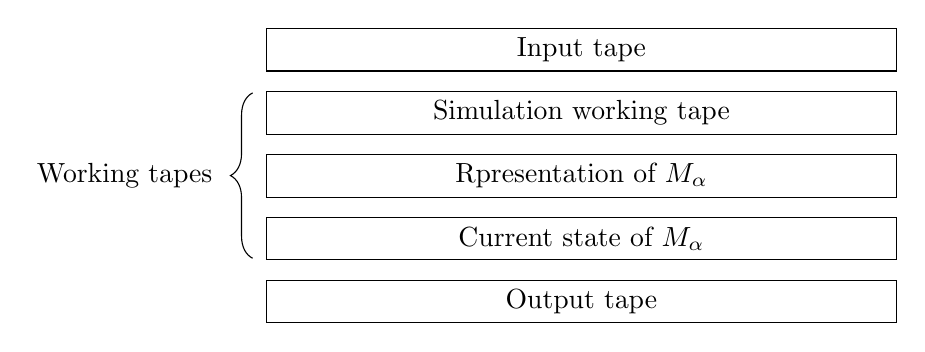
\begin{tikzpicture}
            \node[rectangle, draw, minimum width=8cm, minimum height=0.5 cm] (t1) at (0, 3.2) {Input tape};
            \node[rectangle, draw, minimum width=8cm, minimum height=0.5 cm] (t2) at (0, 2.4) {Simulation working tape};
            \node[rectangle, draw, minimum width=8cm, minimum height=0.5 cm] (t3) at (0, 1.6) {Rpresentation of $M_{\alpha}$};
            \node[rectangle, draw, minimum width=8cm, minimum height=0.5 cm] (t4) at (0, 0.8) {Current state of $M_{\alpha}$};
            \node[rectangle, draw, minimum width=8cm, minimum height=0.5 cm] (t5) at (0, 0.0) {Output tape};

            \draw[decorate, decoration={brace, raise=5pt, amplitude=8pt}] (-4, 0.55) -- (-4, 2.65) node[pos=0.5, left=16pt] {Working tapes};
        \end{tikzpicture}
        \caption{Universal Turing Machine}
        \label{fig:universal-turing-machine}
    \end{figure}
\end{proof}

\begin{rmk}
    In fact, the time bound can be improved using a more complicated encoding $\alpha$, such that if $M_{\alpha}$ halts on input $x$ within $T$ steps, then $U(x, \alpha)$ halts within $C_{\alpha}T\ln(T)$ steps for some $C_{\alpha} \in \N$.
\end{rmk}

\begin{thm}
    There exists a language that is not Turing recognizable.
\end{thm}

\begin{proof}
    Let $A$ be the set of all Turing machines, and let $L$ be the set of all languages. Since we can encode any Turing machine as a finite binary string, we can construct a bijection between the countably infinite set of finite binary strings, and $A$. Therefore $A$ is countable.

    Now, we prove that $L$ is uncountable. Consider the set $F$ of all functions from $\{0, 1\}^{*} \to \{0, 1\}$. We know that there is a bijection between $F$ and $L$, since any language can be uniquely represented as $f \in F$ such that for any finite binary string $w$, $f(w) = 1$ if and only if $w \in L$. Additionally, there is a bijection between $F$ and $[0, 1] \subset \R$. This is given by $f \in F \mapsto 0.f(w_0)f(w_1)\cdots f(w_n)\cdots \in [0, 1]$, where $w_0 = \emptystring$, $w_1 = 0$, $w_2 = 1$, $w_3 = 00$, etcetera. If $f_1 \mapsto r$ and $f_2 \mapsto r$, then $f_1(w) = f_2(w)$ for all finite binary strings $w$, and so $f_1 = f_2$. Furthermore, for any number $r \in [0, 1]$ we can explicitly construct $f$ from $r$. The necessary bijection between $[0, 1]$ and the set $T$ of all infinite binary strings, as well as the uncountability of $[0, 1]$ follows from Cantor's Diagonal Argument \ref{reals-uncountable}. We can then compose the bijections between $L$ and $F$, $F$ and $T$, and $T$ and $[0, 1]$ to obtain a bijection between $L$ and $[0, 1]$. Since $[0, 1]$ is uncountable, it follows that $L$ is as well.

    For any Turing machine $M \in A$, consider the language of all strings it recognizes. Since $A$ is countable but $L$ is not, this mapping cannot be surjective and so there exists a language that is not recognized by any Turing machine.
\end{proof}

\begin{lemma}\label{halting-lemma}
    For any $\alpha \in \{0, 1\}^{*}$, let $M_{\alpha}$ be the Turing machine encoded by $\alpha$. Define a Boolean function $UC$ such that $UC(\alpha) = 0$ if $M_{\alpha}$ accpts input $\alpha$, and $UC(\alpha) = 1$ otherwise (rejects or never halts). Let $L(UC)$ be the language of all strings $w$ such that $UC(w) = 1$.

    Then $L(UC)$ is not Turing recognizable.
\end{lemma}

\begin{proof}
    Assume, for the sake of contradiction, that $L(UC)$ is recognized by a Turing machine $M$ with encoding $\alpha$. Then $UC(\alpha) = 1$ if and only if $M$ accepts $\alpha$. However, $UC(\alpha)$ is defined to be $0$ if $M$ accepts. Therefore, $M$ can neither accept nor reject nor not halt on $\alpha$, and so no such $M$ exists.
\end{proof}

\begin{thm}\label{halting-problem}
    Let \verb|HALT| be the language consisting of all $\langle \alpha, x \rangle$ such that $M_{\alpha}$ halts on input $x$. Here, $\langle \alpha, x \rangle$ uses an encoding $\alpha$ for $M_{\alpha}$ such that a Turing machine can easily check if the input string begins with a valid encoding.

    Then \verb|HALT| is not Turing decidable.
\end{thm}

\begin{proof}
    Assume, for the sake of contradiction, that \verb|HALT| is Turing decidable by a Turing machine $M$ with encoding $\alpha$. Then construct the function $UC$ as follows: for given $\alpha$, use $M$ to determine if $M_{\alpha}$ will halt on input $\alpha$. If not, define $UC(\alpha) = 1$. If it does halt, simulate $\alpha$ until it halts, and define $UC(\alpha) = 0$ if it accepts and $UC(\alpha) = 1$ otherwise. Since we can simulate $\alpha$ using a Turing machine, this would allow use to construct a Turing machine that recognizes $L(UC)$ (in fact, decides it). However, this is a contradiction by Lemma \ref{halting-lemma}, and so \verb|HALT| cannot be decidable.
\end{proof}

\begin{rmk}
    This theorem essentially states no computable algorithm exists which can determine whether a Turing machine will halt on a given input, for all possible inputs and Turing machines. Such an algorithm may exist for some Turing machines and some inputs, but no such algorithm is universal.
\end{rmk}

\begin{prop}
    Let $A_{TM}$ be the language consisting of all $\langle M, \alpha \rangle$ such $M$ accepts $\alpha$. Then $A_{TM}$ is not decidable.
\end{prop}

\begin{proof}
    Assume, for the sake of contradiction, that there exists a Turing machine $M$ that decides $A_{TM}$. Define $UC(\alpha)$ to be $0$ if $M_{\alpha}$ accepts $\alpha$ and $1$ otherwise. We could then trivially compute this using $M$, which contradicts Lemma \ref{halting-lemma}.
\end{proof}

\begin{defn}
    A function $f$ $\Sigma^{*} \to \Sigma^{*}$ is \emph{computable} when there exists a Turing machine $M$ such that for any $w \in \Sigma^{*}$, $M$ will halt with its tape containing $f(w)$.
\end{defn}

\begin{defn}
    Consider languages $A$ and $B$. A \emph{mapping reduction} from $A$ to $B$ is a computable function $f: \Sigma^{*} \to \Sigma^{*}$ such that for any $w \in \Sigma^{*}$, $w \in A \iff f(w) \in B$. If a mapping reduction exists, we write $A \leq_{m} B$ and say that $A$ is \emph{mapping reducible} to $B$.
\end{defn}

\begin{thm}\label{mapping-reduction-decidability}
    Consider languages $A$ and $B$ such that $A \leq_m B$. If $B$ is decidable, then $A$ is decidable.
\end{thm}

\begin{proof}
    Let $M_1$ be a Turing machine which computes the reduction from $A$ to $B$. If $B$ is decided by a Turing machine $M_2$, then $M_2 \odot M_1$ is a Turing machine which decides $A$, so $A$ is decidable.
\end{proof}

\begin{thm}
    $A$ is decidable if and only if $A$ and $\complementof{A}$ are both Turing recognizable.
\end{thm}

\begin{proof}
    If $A$ and $\complementof{A}$ are recognized by Turing machines $M_1$ and $M_2$, we can construct a Turing machine $M$ which alternates running steps of $M_1$ and $M_2$ on separate tapes. If $w \in A$, then $M_1$ will accept, so $M$ accepts. If $w \not\in A$, then $w \in \complementof{A}$ so $M_2$ accepts and $M$ rejects. Therefore, $M$ decides $A$.

    If $A$ is decided by a Turing machine $M$, then $A$ is trivially recognizable. Let $M'$ reject when $M$ accepts and accept when $M$ rejects, and be identical otherwise. Then $M'$ decides $\complementof{A}$.
\end{proof}

\begin{exmp}
    Consider $E_{\textrm{TM}} = \left\{\langle M \rangle : L(M) = \emptyset\right\}$. Notice that the mapping $\langle M, \alpha \rangle \mapsto \langle M \rangle$ is \emph{almost} a mapping reduction from $A_{\textrm{TM}}$ to $\complementof{E_{\textrm{TM}}}$. We just neeed to tweak it slightly so that if $M$ does not accept $\alpha$ then $L(M) = \emptyset$. So define $f(\langle M, \alpha \rangle)$ to be the Turing machine that accepts $\alpha$ if and only if $M$ accepts $\alpha$, and rejects all other inputs. Then clearly $f(\langle M, \alpha \rangle) \in \complementof{E_{\textrm{TM}}}$ if and only if $\langle  M, \alpha \rangle \in A_{\textrm{TM}}$, so $f$ is a mapping reduction from $A_{\textrm{TM}}$ to $\complementof{E_{\textrm{TM}}}$.

    Since $A_{\textrm{TM}}$ is undecidable it follows that $\complementof{E_{\textrm{TM}}}$ is undecidable by Theorem \ref{mapping-reduction-decidability}, and therefore $E_{\textrm{TM}}$ is undecidable.
\end{exmp}

\begin{exmp}
    Consider $R_{\textrm{TM}} = \left\{\langle M \rangle : L(M) \textrm{ is a regular language}\right\}$. Consider $f(\langle M, \alpha \rangle) = M'$, where on input $\beta$, $M'$ runs $M$ on $\alpha$. If $M$ accepts $\alpha$, $M'$ accepts $\beta$ if it is a palindrome, and rejects otherwise. If $M$ rejects $\alpha$, $M'$ rejects all inputs. Therefore, if $\alpha \not\in L(M)$ then $L(M') = \emptyset$ (even if $M$ nevers halts since then neither does $M'$), and if $\alpha \in L(M)$ then $L(M')$ is the non-regular language of palindromes. It follows that $L(M')$ is regular if and only if $\alpha \not\in L(M)$. Therefore, we have a mapping reduction from $A_{\textrm{TM}}$ to the complement of $R_{\textrm{TM}}$, and so $R_{\textrm{TM}}$ is indeed undecidable.
\end{exmp}

\begin{defn}
    A \emph{non-deterministic} Turing machine uses a non-deterministic finite automaton as the control automaton. A non-deterministic Turing machine accepts an input if there exists a sequence of valid transitions for that machine that ends with the accept state, and rejects if all possible such sequences end with the reject state.
\end{defn}

\begin{defn}
    Let $N$ be a non-deterministic Turing machine. We say $N$ runs in time $f(n)$ if every valid sequence of transitions for any input of length $n$ has at most $f(n)$ transitions.
\end{defn}

\section{Complexity theory}

\begin{defn}
    \verb|DTIME|
\end{defn}

\begin{defn}
    Class P
\end{defn}

\begin{defn}
    Class NP
\end{defn}

\begin{exmp}
    Consider the language of strings $\langle G, k \rangle$ such that $G$ is an (encoding of) a graph with an independent set of size $k$. This language is in $NP$, since a list of $k$ vertices forming an independent set can be easily verified in polynomial time.
\end{exmp}

\begin{thm}
    \begin{align*}
        P \subseteq &NP \subseteq EXP \\
        P \subsetneq &EXP
    \end{align*}
\end{thm}

\begin{defn}
    $NP_2$ using non-deterministic Turing machines.
\end{defn}

\begin{thm}
    $NP = NP_2$
\end{thm}

\begin{defn}
    A language $A$ is \emph{polynomial-time reducible} to a language $B$ is there exists a mapping reduction of $A$ to $B$ using a function which is computable in polynomial time, written $A \leq_{p} B$.
\end{defn}

\begin{prop}
    If $L$ is polynomial-time reducible to $L'$, and $L' \leq_{p} L''$, then $L \leq_{p} L''$.
\end{prop}

\begin{defn}
    NP-hard is the class of languages $L$ such that any language in NP is polynomial-time reducible to $L$.
\end{defn}

\begin{defn}
    A language is NP-complete if it is both NP-hard and in NP.
\end{defn}

\begin{thm}\proofbreak
    \begin{itemize}
        \item If $L$ is in NP-hard and in P, then $P = NP$.
        \item If $L$ is NP-complete, then $L \in P$ if and only if $P = NP$.
    \end{itemize}
\end{thm}

\begin{defn}
    A Boolean formula with literals (Boolean variables) $x_1, \ldots, x_n $ is \emph{satisfied} by an \emph{assignment} of truth values $z_1, \ldots, z_n$ to its literals if it evaluates to \textsc{true}. A Boolean formula is \emph{satisfiable} if there exists an assignment which satisfies it.
\end{defn}

\begin{defn}
    A Boolean formula is in \emph{conjunctive normal form} (CNF) if it is a conjunction of one or more disjunctions of one or more literals or negation of literals. In other words, it is an \verb|AND| of \verb|OR|s.

    A Boolean formula is in \emph{disjunctive normal form} (DNF) if it is a disjunction of one or more conjunctions of one or more literals or negation of literals. In other words, it is an \verb|OR| of \verb|AND|s.

    The size of a formula is the sum of the length of clauses, where the length of a clause is the number of literals.
\end{defn}

\begin{lemma}\label{function-to-cnf}
    We can express any Boolean function $f: \{0, 1\}^{\ell} \to \{0, 1\}$ as a $\ell$ variable formula in CNF with at most $\ell 2^{\ell}$ clauses.
\end{lemma}

\begin{proof}
    Let $f: \{0, 1\}^{\ell} \to \{0, 1\}$. We will express this as a CNF formula with literals $x_1, \ldots, x_{\ell}$, where the string $x_1x_2\cdots x_{\ell}$ is the input to $f$. Let $A$ be the set of all strings $\omega$ such that $f(\omega) = 0$.

    For any $\omega = \omega_1\ldots \omega_{\ell} \in A$, let $a_i = x_i$ if $\omega_i = 0$ and $a_i = \neq x_i$ if $\omega_i = 1$. Consider the clause $a_1 \lor a_2 \lor \cdots \lor a_{\ell}$. If this clause is true, then $x_1\ldots x_{\ell}$ must differ from $\omega$ in at least one position. Since $|A| \leq 2^{\ell}$, we can enumerate all such clauses as $c_1, \ldots, c_{k}$ where $k \leq 2^{\ell}$. Then the CNF formula
    \begin{align*}
        c_1 \land c_2 \land \cdots \land c_{k}
    \end{align*}
    is equivalent to $f(\omega)$, since it is true precisely when $\omega \not\in A$.

    Note that every clause contains exactly $\ell$ literals, and there are $k \leq 2^{\ell}$ clauses. Therefore, the overall formula has size at most $\ell 2^{\ell}$.
\end{proof}

\begin{defn}
    SAT is the language of all satisfiable CNF Boolean formulas. 3-SAT is the language of all satisfiable CNF Boolean formulas, where each clause has length at most three.
\end{defn}

\begin{lemma}\label{CNF-to-3-CNF}
    Let $X$ be a CNF formula with size $n$, then there exists a 3-CNF formula which is satisfiable if and only if $X$ is satisfiable, and whose size is polynomial in $n$.
\end{lemma}

\begin{proof}
    Consider any clause $x_1 \lor x_2 \lor x_3 \lor \cdots \lor x_n$. Notice that this is equivalent to
    \begin{align*}
        (x_1 \lor x_2 \lor y) \land (\neg y \lor x_3 \lor \cdots \lor x_n),
    \end{align*}
    which has two clauses of size three and $n-1$. Therefore, we can recursively reduce $X$ to a 3-CNF formula by breaking apart every clause with length longer than three. Every clause of length $k > 3$ is reduced to a 3-CNF formula of size $3(k-3) + 3 = 3(k-2)$. Therefore, a CNF formula $X$ of size $n$ can be reduced to a formula of size at most $3(n-2)$, since the worst case occurs when $X$ contains a single clause of length $n$.
\end{proof}

\begin{thm}{Cook-Levin theorem}\proofbreak
    Both SAT and 3-SAT are NP-complete.
\end{thm}

\begin{proof}
    SAT and 3-SAT are in NP, because a certificate consisting of an assignment of the variables can be easily verified in polynomial time.

    For any language $L$ in NP, by definition there exists a polynomial function $p: \N \to \N$ and polynomial time Turing machine $M$ such that $x \in \{0, 1\}^{*}$ is in $L$ if and only if there exists $u$ of length at most $p(\abs{x})$ such that $M(x, u) = 1$. Note that for fixed $x$, $M(x, u)$ is equivalent to $M'(u)$ for some $M'$, and is therefore equivalent to $\phi(u)$ for some binary function $\phi$. By Lemma \ref{function-to-cnf}, $\phi$ can be expressed as a CNF formula, however this is not necessarily computable in polynomial time since the formula can have size $|x|2^{|x|}$.

    Consider the following polynomial-time computable construction of a CNF formula from the Turing machine $M$. We know that $M(x, u) = 1$ if and only if there exists a sequence of configurations $C_0, \ldots, C_t$ such that $C_0$ is the start configurtion, $C_T$ is an accept configuration, and $C_i \to C_{i+1}$ obeys the transition function. Note that $T$ is bounded by the running time of $M$, which is polynomial. For all $C_i$, let $z_i$ be a set of Boolean variables describing the $C_i$, including head positions, control automaton state, and tape states, and let $u_1, \ldots, u_k$ such that $u = u_1\cdots u_k$ is the certificate. Since the tapes of $C_i$ and $C_{i+1}$ can only differ in a single window of length three around the head position, we can verify a transition by checking that all but one window remains the same, and the window which changes obeys the transition function.

    The full details are exceedingly complex, see the Cook-Levin Theorem in Chapter 7 of Sipser's ``Introduction to the Theory of Computation'', 3rd edition, for some of these details. Essentially, a CNF formula can be constructed in polynomial time that states whether a series of configurations is equivalent to the computation of $M(x, u)$, where $M(x, u)$ accepts. Therefore, the satisfiability of this CNF problem is equivalent to deciding $x$, and since it is done with a polynomial-time reduction, SAT is NP-hard by definition, and therefore NP-complete.

    Finally, we show that SAT is polynomial-time reducible to 3-SAT. By Lemma \ref{CNF-to-3-CNF}, we can compute in polynomial-time a reduction of any CNF formula to a 3-CNF formula, and so $\textrm{SAT} \leq_{p} \textrm{3-SAT}$, so 3-SAT is NP-hard.
\end{proof}

\begin{thm}\label{dhampath-np-complete}
    The language of graphs which contain Hamiltonian paths, \verb|dHAMPATH|, is NP-complete.
\end{thm}

\begin{thm}\label{dhamcycle-np-complete}
    The language of graphs which contain Hamiltonian cycles, \verb|dHAMCYCLE|, is NP-complete.
\end{thm}

\begin{proof}
    Given a graph $G$, construct $G'$ with a two new vertices $v_{start}$ and $v_{end}$ such that every vertex has an edge to $v_{end}$, $v_{end}$ has an edge to $v_{start}$, and $v_{start}$ has an edge to every other vertex. If $G$ has a Hamiltonian path, prefixing $v_{start}$ and suffixing $v_{end}$ to this path produces a Hamiltonian cycle in $G'$. If $G'$ has a Hamiltonian cycle, then it must use the edge from $v_{end}$ to $v_{start}$, and so shifting the cycle to make $v_{end}$ the final vertex, and then removing $v_{end}$ and $v_{start}$ produces a Hamiltonian path in $G$. Therefore $G$ has a Hamiltonian path if and only if $G'$ has a Hamiltonian cycle. Since we can easily construct $G'$ from $G$ in polynomial time, \verb|dHAMPATH| is then polynomial-time reducible to \verb|dHAMCYCLE| and so \verb|dHAMCYCLE| is NP-hard by Theorem \ref{dhampath-np-complete}. Finally, we can easily verify Hamiltonian cycles in polynomial time, and so \verb|dHAMCYCLE| is NP-complete.
\end{proof}

\begin{thm}{Traveling salesman problem}\proofbreak
    Given a weighted, directed, complete graph $G$ on $n$ vertices, the problem of deciding whether $G$ contains a Hamiltonian cycle of length at most $k$ is NP-complete.
\end{thm}

\begin{proof}
    A certificate consiting of a Hamiltonian cycle of length at most $k$ can be easily verified in polynomial time.

    Let $G$ be a directed graph. Construct $G'$ to be a weighted, directed, complete graph where an edge has weight $1$ if it was not in $G$ and $0$ otherwise, and take $k = 0$. Then a Hamiltonian cycle in $G$ is a Hamiltonian cycle in $G'$ of length at most $k$, and a Hamiltonian cycle in $G'$ of length at most $k=0$ clearly cannot use edges not in $G$, and so is also a Hamiltonian cycle in $G$. Since constructing this graph can in done in polynomial time, \verb|dHAMCYCLE| is polynomial-time reducible to the traveling salesman problem, and so by Theorem \ref{dhamcycle-np-complete} the traveling salesman problem must be NP-complete.
\end{proof}

\begin{thm}
    If there exists an algorithm which decides SAT, then there exists an algorithm which for CNF $\phi$ in SAT can \emph{find} an assignment that satisfies $\phi$.
\end{thm}

\begin{proof}
    Let $A$ be an algorithm which decides SAT. Then the following algorithm can find satisfying assignments.

    Let $\phi$ be a CNF formula with $n$ variables $x_1, \ldots, x_n$. Determine whether $\phi$ is in SAT using $A$. If not, halt. Otherwise, assign $0$ to $x_1$ and determine whether the reduced formula is in SAT. If not, since a satisfying assignment exists, assign $1$ to $x_1$. We have, by running $A$ once, reduced $\phi$ to having $n-1$ variables. We then simply repeat this procedure $n-1$ more times to determine a satisfying assignment, which takes $n+1$ total calls to $A$. Assuming $A$ runs in time $T(n)$, the algorithm runs in $O(nT(n))$, which is polynomial if $T(n)$ is.
\end{proof}

\input{groups}
\documentclass[12pt]{article}

\usepackage{amsmath}
\usepackage{amssymb}
\usepackage{amsthm}
\usepackage{centernot}
\usepackage{fullpage}
\usepackage{makecell}
\usepackage{tabularx}
\usepackage[hypcap=false]{caption}
\usepackage{tikz, tkz-euclide}
\usetikzlibrary{decorations.pathreplacing,arrows}
\usetikzlibrary{quotes,angles,calc,intersections}

\usepackage{titling}
\usepackage{pdfpages}
\usepackage{enumitem}
\usepackage{multicol}
\usepackage{bm}

\usepackage{linear}
\usepackage{common}

\begin{document}

\title{Ordinary Differential Equations}
\author{Brendan Burkhart}
\maketitle

\tableofcontents
\newpage

\section{Classification}

\begin{defn}
    A \emph{differential equation} is an equation relating one or more independent variables, functions of those variables, and derivatives of those functions.
\end{defn}

\begin{exmp}\label{first-order-ode}
    \[\frac{\mathrm{d}x}{\mathrm{d}t} = x\]
\end{exmp}

\begin{defn}
    A \emph{solution} to a differential equation is an expression for the dependent functions of the differential equation in terms of the independent variables.
\end{defn}

Differential equations can be broadly classified into \emph{ordinary} and \emph{partial} differential equations.

\begin{defn}
    An \emph{ordinary} differential equation, or \emph{ODE} is a differential equation involving a single independent variable, and all derivatives are with respect to this variable.
\end{defn}

\begin{defn}
    A \emph{partial} differential equation, or \emph{PDE} is a differential equation involving functions of more than one independent variables, and derivatives may be with respect to any of those variables.
\end{defn}

\begin{defn}
    The \emph{general form} of an ODE is
    \[F(x, y, y', \ldots, y^{(n)}) = 0,\] that is some expression involving the independent variable $x$, the dependent variable $y$, and the derivatives of $y$.
\end{defn}

\begin{defn}
    The \emph{order} of a differential equation is the order of the highest derivative.
\end{defn}

\begin{exmp}
    \[\frac{\mathrm{d}^2\theta}{\mathrm{d}t^2} + \frac{g}{L}\sin\theta = 0\]
    This is a second order differential equation, while Example \ref{first-order-ode} is first order.
\end{exmp}

\begin{defn}
    A differential equation of a dependent variable $y$ and its derivatives is said to be \emph{linear} if it is an affine map with regard to $y$ and its derivatives.
\end{defn}

\begin{exmp}
    $\sin(x)y' + 2x^2y'' = x$ is linear.
\end{exmp}

\begin{exmp}
    $yy' + y'' = 0$ is non-linear.
\end{exmp}

\begin{defn}
    An \emph{autonomous} differential equation is one in which the independent variable does not explicitly appear. When the independent variable represents time in some way, these may also be called \emph{time-invariant}.
\end{defn}

\begin{exmp}
    $\frac{\mathrm{d}y}{\mathrm{d}x} = 5y - 20$ is an autonomous differential equation as the independent variable $x$ is not explicitly present.
\end{exmp}

\section{First-order linear autonomous differential equations}

Any first-order linear autonomous differential equation with independent variable $x$ and dependent variable $y$ can trivially be put into the form \[\frac{\mathrm{d}y}{\mathrm{d}x} = ay - b.\] This form can always be solved.

\begin{align*}
    \frac{\mathrm{d}y}{\mathrm{d}x} &= ay - b \\
    &= a(y - \frac{b}{a})
\end{align*}

Note that $\frac{\mathrm{d}}{\mathrm{d}x}{y - \frac{b}{a}} = \frac{\mathrm{d}}{\mathrm{d}x}y$. If $y \neq \frac{b}{a}$, it follows that $\ln(y - \frac{b}{a}) = ax + C$ for some constant of integration $C$, so $\abs{y - \frac{b}{a}} = ke^{ax}$ for some $k$. If $y > \frac{b}{a}$, then $y = \frac{b}{a} + ke^{ax}$, and similarly if $y < \frac{b}{a}$, then $y = \frac{b}{a} + ke^{ax}$ for some $k$. In the case that $y = \frac{b}{a}$, it follows that $\frac{\mathrm{d}y}{\mathrm{d}x} = 0$, so $y = \frac{b}{a} + ke^{ax}$ where $k = 0$.

Therefore, $y = \frac{b}{a} + ke^{ax}$ is a solution to any first-order linear autonomous differential equation.

\end{document}

\setchaptergraphic{
    % Hyperboloid of one sheet
    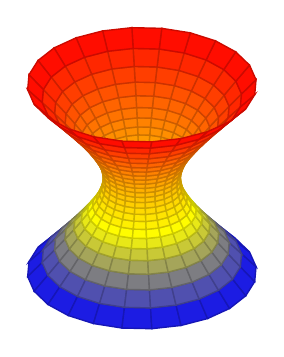
\begin{tikzpicture}[scale=1.25]
        \begin{axis}[hide axis,axis equal,colormap/hot]
            \addplot3[surf,domain=0:360,y domain=-1.75:1.75] ({cosh(y)*cos(x)},{cosh(y)*sin(x)},{sinh(y)});
        \end{axis}
    \end{tikzpicture}
    \hspace{1cm}
    % Saddle
    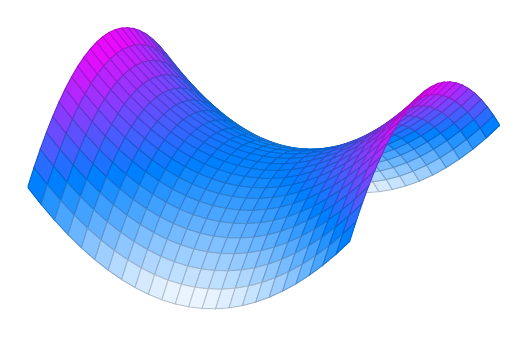
\begin{tikzpicture}[scale=0.875]
        \begin{axis}[hide axis,colormap/cool]
            \addplot3[surf,domain=-1.5:1.5,y domain=-1.5:1.5] {x^2-y^2};
        \end{axis}
    \end{tikzpicture}
}

\chapter{Vector Calculus}
\label{ch:vector-calc}

\section{Orthogonal Projection}

\begin{thm}\label{law-of-cosines}
    Let $\theta$ be the angle between non-zero vectors $A$ and $B$, and let $C = A - B$. The \emph{Law of Cosines} states that $\norm{C}^2 = \norm{A}^2 + \norm{B}^2 - 2\norm{A}\norm{B}\cos(\theta)$.
\end{thm}

\begin{figure}[ht!]
    \centering
    \begin{tikzpicture}[scale=1.4]
        \coordinate (O) at (0, 0);
        \coordinate (A) at (3, 5);
        \coordinate (B) at (6, 2);
        \coordinate (A') at ($(O)!(A)!(B)$);

        \draw [thick, ->] (O) -- (A);
        \draw [thick, ->] (O) -- (B);
        \draw [thick, dashed] (A') -- (A);
        \draw [very thick, red, ->] (O) -- (A');

        \draw [decorate,decoration={brace,amplitude=6pt,raise=3pt]}]
            (O) -- (A) node [black,midway,xshift=-0.6cm,yshift=0.3cm]
            {\footnotesize $A$};

        \draw [decorate,decoration={brace,amplitude=6pt,raise=3pt]}]
            (B) -- (O) node [black,midway,xshift=0.2cm,yshift=-0.5cm]
            {\footnotesize $B$};

        \draw [decorate,decoration={brace,amplitude=6pt,raise=3pt]}]
            (A) -- (A') node [black,midway,xshift=1.0cm, yshift=0.1cm]
            {\footnotesize $A - A'$};

        \draw [decorate,decoration={brace,amplitude=6pt,raise=3pt]}]
            (O) -- (A') node [black,midway,xshift=-0.2cm, yshift=0.5cm]
            {\footnotesize $A'$};

        \tkzMarkAngle[size=1cm,mark=|](B,O,A)
        \tkzLabelAngle[pos=1.2](B,O,A) {$\theta$}

        \tkzMarkRightAngle[size=0.4](A,A',O)
    \end{tikzpicture}
\caption{Orthogonal projection of $\vec{A}$ onto $\vec{B}$}
\label{fig:orthogonal-projection}
\end{figure}

Figure \ref{fig:orthogonal-projection} shows $A'$, the orthogonal projection of vector $A$ onto $B$. $\norm{A'}$ is the shortest distance between the head of $A$ and $B$.

\begin{thm}
    Let $\theta$ be the angle between non-zero vectors $A$ and $B$. Then $\cos\theta = \frac{A \cdot B}{\norm{A}\norm{B}}$.
\end{thm}

\begin{proof}\label{vector-angle}
    Let $C = A - B$. Then $C \cdot C = (A - B) \cdot (A - B)$, which can we expand to get $A \cdot (A - B) - B \cdot (A - B) = A \cdot A + B \cdot B - 2(A \cdot B)$. Therefore, $\norm{C}^2 = \norm{A}^2 + \norm{B}^2 - 2(A \cdot B)$. By the Law of Cosines \ref{law-of-cosines} and transitivity, it follows that $A \cdot B = \norm{A}\norm{B}\cos\theta$, so $\cos\theta = \frac{A \cdot B}{\norm{A}\norm{B}}$.
\end{proof}

\begin{exmp}
    Let $A = \left(0, 1\right)$, and $B = \left(2, 2\right)$. Then $\cos\theta = \frac{A \cdot B}{\norm{A}\norm{B}}$. Since $A \cdot B = 0 \cdot 2 + 1 \cdot 2 = 2$, $\norm{A} = \sqrt{0^2 + 1^2} = 1$, and $\norm{B} = \sqrt{2^2 + 2^2} = \sqrt{8} = 2\sqrt{2}$, we have $\cos\theta = \frac{2}{1 \cdot 2\sqrt{2}}$. This is equal to $\frac{\sqrt{2}}{2}$, so $\theta = \frac{\pi}{4}$.
\end{exmp}

\begin{exmp}
    Let $A = {1, 1}$ and $B = {1, -1}$. Then since $A \cdot B = 1 - 1 = 0$, we know $\cos\theta = 0$, which implies that $\theta = \frac{\pi}{2}$.
\end{exmp}

\begin{cor}\label{orthogonal-vectors}
    Non-zero $A$ and $B$ are orthogonal if and only if $A \cdot B = 0$.
\end{cor}

\begin{proof}
    Let $A$ and $B$ be non-zero orthogonal vectors. Then the angle ($\theta$) between $A$ and $B$ must be $\frac{\pi}{2}$ since they are orthogonal. By Theorem \ref{vector-angle}, $\cos\theta = \frac{A \cdot B}{\norm{A}\norm{B}}$. Since $A$ and $B$ are non-zero, $\norm{A}\norm{B}$ is non-zero, and since $\theta = \frac{\pi}{2}$, we know $\cos\theta = 0$. Therefore, $A \cdot B$ must equal zero.
\end{proof}

\begin{thm}\label{vector-projection}
    Let $A$ and $B$ be vectors, and $A'$ be the orthogonal projection of $A$ onto $B$. Then $A' = \frac{A \cdot B}{B \cdot B}B$.
\end{thm}

\begin{proof}
    Let $d \in \R$ such that $C = dB$. Then since $(A - dB) \cdot B = 0$, we know $A \cdot B - dB \cdot B = 0$, so $A \cdot B = d(B \cdot B)$. This implies that $d = \frac{A \cdot B}{B \cdot B}$. Since $C = dB$, we then have $C = \frac{A \cdot B}{B \cdot B}B$.
\end{proof}

\begin{exmp}
   Let $A = \left(2, 2\right)$, and $B = \left(1, 0\right)$. Then since $A \cdot B = 2$, and $B \cdot B = 1$, we know $A' = \frac{2}{1}B = \left(2, 0\right)$.
\end{exmp}

\begin{thm}
    Let $p$ be a point, and $A\cdot\vec{x} + D = 0$ be a plane. Then the distance from the point to the plane is given by $\frac{A\cdot p + D}{\norm{A}}$.
\end{thm}

\begin{proof}
    The line with direction $A$ that passes through $p$ is normal to the plane and thus contains the shortest path from the point to the plane. Therefore, $A \cdot (p + tA) + D = 0$ gives the closest point on the plane to $p$. We then have $A \cdot p + D = -t(A \cdot A)$. Since the shortest distance is equal to $|-t\norm{A}|$, it follows that the shortest distance is given by \[\frac{\abs{A \cdot p + D}}{\norm{A}}.\]
\end{proof}

\begin{cor}
    Let $(x_1, y_1, z_1)$ be a point in $\R^3$, and $Ax + By + Cz + D = 0$ be a plane in $\R^3$. Then the distance from the point to the plane is: \[\frac{\abs{Ax_1 + By_1 + Cz_1 + D}}{\sqrt{A^2 + B^2 + C^2}}.\]
\end{cor}

\section{Cross Product}

\begin{defn}
    The \emph{cross product} or \emph{vector product} of three-dimensional vectors $A = a_1i + a_2j + a_3k$ and $B = b_1i + b_2j + b_3k$ is written $A \times B$. \[A \times B = \begin{vmatrix}
        i & j & k \\ a_1 & a_2 & a_3 \\ b_1 & b_2 & b_3
    \end{vmatrix}\] The value of this determinant can be found via the Laplace formula (also called cofactor expansion) along any column or row. Expansion along the first row gives: \[A \times B =
    \begin{vmatrix}
        i & j & k \\ a_1 & a_2 & a_3 \\ b_1 & b_2 & b_3
    \end{vmatrix} =
    \begin{vmatrix}
        a_2 & a_3 \\ b_2 & b_3
    \end{vmatrix}i -
    \begin{vmatrix}
        a_1 & a_3 \\ b_1 & b_3
    \end{vmatrix}j +
    \begin{vmatrix}
        a_1 & a_2 \\ b_1 & b_2
    \end{vmatrix}k\] \[= (a_2b_3 - b_2a_3)i - (a_1b_3 - b_1a_3)j + (a_1b_2 - b_1a_2)k.\]
\end{defn}

\begin{rmk}
    The cross product is a non-commutative binary operation.
\end{rmk}

\begin{exmp}
    Let $A = 3i + j - k$, and $B = -6i - 2j - 2k$. Then \[A \times B =
    \begin{vmatrix}
        i & j & k \\ 3 & 1 & -1 \\ -6 & -2 & -2
    \end{vmatrix} = (-2 - 2)i - (-6 - 6)j + (-6 + 6)k = -4i + 12j + 0k.\]
\end{exmp}

\begin{thm}
    Let $A = a_1i + a_2j + a_3k$ and $B = b_1i + b_2j + b_3k$ be vectors. Then $A \times B$ is orthogonal to both $A$ and $B$.
\end{thm}

\begin{proof}
    Since $A \times B = (a_2b_3 - b_2a_3)i - (a_1b_3 - b_1a_3)j + (a_1b_2 - b_1a_2)k$, we know that $A \cdot (A \times B) = (a_1a_2b_3 - a_1b_2a_3) - (a_1a_2b_3 - b_1a_2a_3) + (a_1b_2a_3 - b_1a_2a_3)$. This is equal to $(a_1a_2b_3 - a_1a_2b_3) - (b_1a_2a_3 - b_1a_2a_3) + (a_1b_2a_3 - a_1b_2a_3)$, which is equal to $0$, so by Corollary \ref{orthogonal-vectors} we know $A$ is orthogonal to $A \times B$. Similarly, $B$ is orthogonal to $A \times B$.
\end{proof}

\begin{thm}
    Let $A$, $B$, and $C$ be vectors, and $x$ a real number. Then:
    \begin{itemize}
        \item $A \times B = \vec{0}$ if and only if $A = \vec{0}$, $B = \vec{0}$, or $A$ is parallel to $B$.
        \item $A \times B = -(B \times A)$.
        \item $A \times (B + C) = (A \times B) + (A \times C)$.
        \item $(A + B) \times C = (A \times C) + (B \times C)$.
        \item $(\alpha A) \times B = A \times (\alpha B) = \alpha(A \times B)$.
    \end{itemize}
\end{thm}

\begin{rmk}
    In a \emph{right-handed} coordinate system, the cross product will follow the \emph{right-hand rule}: on the right hand, index finger represents $A$, middle finger represents $B$, and then thumb represents $A \times B$. However, in a \emph{left-handed} coordinate system, the cross product will instead follow the similar \emph{left-hand rule}. The chirality of the cross product follows the chirality of the chosen basis, and is not inherently due to the definition of the cross product.
\end{rmk}

\begin{thm}
    Let $A$ and $B$ be two vectors, and $\theta$ be the angle between them. Then $\norm{A \times B} = \norm{A}\norm{B}\sin\theta$, which is the area of a parallelogram with side lengths $\norm{A}$ and $\norm{B}$ and angle $\theta$.
\end{thm}

\begin{thm}
    The shortest distance between two non-parallel lines $p_1 + t_1d_1$ and $p_2 + t_2d_2$ is given by \[\frac{(p_1 - p_2) \cdot (d_1 \times d_2)}{\norm{d_1 \times d_2}}.\]
\end{thm}

\begin{proof}
    The shortest distance must lay on a vector that is orthogonal to both lines, which would be $d_1 \times d_2$. The component of $p_1 - p_2$ onto $d_1 \times d_2$ is then the shortest distance between the lines.
\end{proof}

\begin{thm}
    The closest point on a line $p_1 + t_1d_1$ to another lines $p_2 + t_2d_2$ is \[p_1 + \frac{(p_2 - p_1)\cdot n}{d_1 \cdot n}d_1.\]
\end{thm}

\begin{proof}
    The vector between the closest point and $p_2$ must be parallel to $d_1 \times d_2$, so it will intersect the plane with normal $(d_1 \times d_2) \times d_2$. Let $n = (d_1 \times d_2) \times d_2$. Then \[\left\{(p_1 + t_1d_1) - p_2\right\} \cdot n = 0,\] so $(p_2 - p_1)\cdot n = t(d_1 \cdot n)$. Therefore, the closest point is given by \[p_1 + \left(\frac{(p_2 - p_1)\cdot n}{d_1 \cdot n}\right)d_1.\]
\end{proof}

\section{Alternative Coordinate Systems}

There are many useful alternatives to the Cartesian coordinate system, such as the polar, cylindrical, and spherical coordinate systems.

In polar coordinates, two-dimensional points are represented by a radius $r$ and an angle $\theta$. The $r$ is the radius from the origin, and $\theta$ is the angle measured anticlockwise around the origin, starting from the positive half of the $x$-axis.

\begin{thm}
    Let $(x, y)$ be a point in Cartesian coordinates. Then $(r, \theta)$, where
    \begin{itemize}
        \item $r = \sqrt{x^2 + y^2}$
        \item $\theta = \arctan\frac{y}{x}$
    \end{itemize} gives the same point in polar coordinates.
\end{thm}

\begin{thm}
    Let $(r, \theta)$ be a point in polar coordinates. Then $(x, y)$, where
    \begin{itemize}
        \item $x = r\cos\theta$
        \item $y = r\sin\theta$
    \end{itemize} gives the same point in Cartesian coordinates.
\end{thm}

\begin{exmp}
    $(2, 2)$ in Cartesian coordinates is $(\sqrt{4 + 4}, \arctan(\frac{2}{2})) = (2\sqrt{2}, \frac{\pi}{4})$ in polar coordinates.
\end{exmp}

Since $(r, \theta + 2\pi{n})$ and $(-r, \theta + 2\pi{n})$ represent the same point in polar coordinates for all $n \in \Z$, it is common to choose ranges for $r$ and $\theta$ to make the representation of any given point unique. One such scheme is to restrict $\theta$ to $\left[0, 2\pi\right)$, and $r > 0$ except for the unique origin, $(0, 0)$.

While the two-dimensional Cartesian coordinate system is extended to three dimensions by adding the $z$-axis, there are two different ways to extend the polar coordinate system to three dimensions: cylindrical and spherical coordinates.

In cylindrical coordinates, polar coordinates are augmented with a $z$-axis, so points are represented as $(r, \theta, z)$. The radius, $r$, is still measured within the $xy$ plane.

Let $(x, y, z)$ be a point in the Cartesian coordinate system, and $(r, \theta, z)$ be the same point in cylindrical coordinates. Then all the same relationships are true as for polar coordinates, with the addition that $z = z$.

\begin{exmp}
    $(2, 2, 5)$ in Cartesian coordinates is $(\sqrt{4 + 4}, \arctan(\frac{2}{2}), 5) = (2\sqrt{2}, \frac{\pi}{4}, 5)$ in cylindrical coordinates.
\end{exmp}

In spherical coordinates, polar coordinates are augmented with a zenith angle $\phi$, measured from the zenith ($z$-axis) down to the point. The radius is measured in three dimensions rather than just in the $xy$-plane, so it is typically represented using the symbol $\rho$ rather than $r$ to differentiate it from the polar radius.

\begin{thm}
    Let $(x, y, z)$ be a point in Cartesian coordinates. Then $(\rho, \theta, \phi)$, where
    \begin{itemize}
        \item $\rho = \sqrt{x^2 + y^2 + z^2}$
        \item $\theta = \arctan\frac{y}{x}$
        \item $\phi = \arccos\frac{z}{\rho}$
    \end{itemize} gives the same point in spherical coordinates.
\end{thm}

\begin{thm}
    Let $(\rho, \theta, \phi)$ be a point in spherical coordinates. Then $(x, y, z)$, where
    \begin{itemize}
        \item $r = \rho\sin\phi$
        \item $x = r\cos\theta$
        \item $y = r\sin\theta$
        \item $z = \rho\cos\phi$
    \end{itemize} gives the same point in Cartesian coordinates.
\end{thm}

\begin{exmp}
    If $(\sqrt{6}, -\sqrt{2}, -2\sqrt{2})$ is a point in Cartesian coordinates, then $\rho$ is equal to $\sqrt{6 + 2 + 8} = 4$, $\theta = \arctan\frac{-\sqrt{2}}{\sqrt{6}} = \frac{11\pi}{6}$, and $\phi = \arccos\frac{-2\sqrt{2}}{4} = \frac{3\pi}{4}$.
\end{exmp}

\section{Gradient}

\begin{defn}
    Let $f: \R^n \to \R$. Then the \emph{gradient} of $f$, denoted by $\nabla f$, is a vector representing the derivative of the function: \[\left\langle \frac{\partial f}{\partial x_1}, \frac{\partial f}{\partial x_2}, \ldots, \frac{\partial f}{\partial x_n} \right\rangle.\]
\end{defn}

\begin{defn}
    The \emph{directional derivative} of a function $f: \R^n \to \R$ in the direction given by a unit vector $v$ is $\nabla f \cdot v$.
\end{defn}

\begin{thm}
    The gradient of a function $f: \R^n \to \R$ is the direction that maximizes change.
\end{thm}

\begin{proof}
    Since $x \cdot y = \norm{x}\norm{y}\cos(\theta)$, it follows that the unit vector to maximizes the directional derivative is $\frac{\nabla f}{\norm{\nabla f}}$, as this is when $\cos(\theta)$ is maximized.
\end{proof}

\section{Surfaces}

\begin{defn}
    A \emph{level set} of a real-valued function for a value $c \in \R$ is the set of all points where the value of the function is $c$. For a function $f$ of $n$ real variables, the level set is \[L_c(f) = \left\{\left(x_1, x_2, \ldots, x_n\right) \compbar f(x_1, x_2, \ldots, x_n) = c\right\}.\]
\end{defn}

\begin{rmk}
    When $n = 2$, the level sets are called \emph{level curves}. These as essentially the same as contour lines on a topographical map. When $n=3$, the level sets are called \emph{level surfaces}.
\end{rmk}

\begin{prop}
    The tangent vector to a level set at a specific point is orthogonal to the gradient at that point.
\end{prop}

\begin{proof}
    Since the value of all points in a level set are equal, the directional derivative in the direction of a tangent to a level set must be zero. Let $v$ be a tangent vector at a point $p$. Then $\nabla f(p) \cdot \frac{v}{\norm{v}} = 0$ implies that $\nabla f(p)$ is orthogonal to $v$ by Corollary \ref{orthogonal-vectors}.
\end{proof}

\begin{defn}
    A \emph{cylinder} is a surface that consists of parallel lines that intersect a given plane curve. For a cylinder in the more typical sense, the plane curve is a circle.
\end{defn}

\begin{defn}
    \emph{Quadric surfaces} are higher-dimensional generalizations of conic sections --- ellipses, parabolas, and hyperbolas. In three dimensions with coordinate variables $x, y, z$, quadric surfaces are given by $Ax^2 + By^2 + Cz^2 + Dxy + Exz + Fyz + Gx + Hy + Iz + J = 0$.
\end{defn}

\begin{defn}
    An \emph{ellipsoid} with width ($x$) $a$, height ($y$) $b$, and depth ($z$) $c$ is \[\frac{x^2}{a^2} + \frac{y^2}{b^2} + \frac{z^2}{c^2} = 1.\] This can be decomposed into three orthogonal ellipses by individually setting each coordinate variable to zero.
\end{defn}

\begin{defn}
    A \emph{paraboloid} oriented around the $z$-axis is given by \[\frac{x^2}{a^2} + \frac{y^2}{b^2} = \frac{z}{c}.\] This can be decomposed into ellipses around the $z$-axis, and parabolas along the $x$ and $y$ axes.
\end{defn}

\begin{defn}
    By negating either the $x^2$ or $y^2$ term in a paraboloid, we can form a \emph{saddle}. A saddle the curves up along the $x$ axis and down along the $y$ axis is given by \[\frac{x^2}{a^2} - \frac{y^2}{b^2} = \frac{z}{c}.\]
\end{defn}

\begin{defn}
    A hyperboloid comes in three types, all with the general form \[\frac{x^2}{a^2} + \frac{y^2}{b^2} - \frac{z^2}{c^2} = r,\] if they are aligned with the $z$-axis. When:
    \begin{itemize}
        \item $r > 0$, the hyperboloid is cooling-tower shaped along the $z$-axis, and is known as a hyperboloid of one sheet, or a hyperbolic hyperboloid.
        \item $r = 0$, the hyperboloid is composed of two cones along the $z$-axis, and is known simply as a cone.
        \item $r < 0$, the hyperboloid is vaguely shaped like two separated paraboloids facing away from each other, and is known as a hyperboloid of two sheets, or an elliptic hyperboloid.
    \end{itemize}
\end{defn}

\section{Taylor's Theorem}

Let $f: \R^2 \to \R$ be a $C^2$ (all second derivatives are continuous) function. Then the quadratic Taylor polynomial around $a = (x_0, y_0)$ must be of the form $T_2(x, y) = A + B(x-x_0) + C(y-y_0) + D(x-x_0)(y-y_0) + E(x-x_0)^2 + F(y-y_0)^2$.

Then:
\begin{itemize}
    \item $\frac{\partial T_2}{\partial x} = B + D(y-y_0) + 2E(x-x_0)$,
    \item $\frac{\partial T_2}{\partial y} = C + D(x-x_0) + 2F(y-y_0)$,
    \item $\frac{\partial T_2}{\partial xy} = D$,
    \item $\frac{\partial T_2}{\partial xx} = 2E$,
    \item $\frac{\partial T_2}{\partial yy} = 2F$.
\end{itemize}

Therefore, we have $E = \frac{1}{2}\frac{\partial^2 f}{\partial x^2}(a)$, $F = \frac{1}{2}\frac{\partial^2 f}{\partial y^2}(a)$, $D = \frac{1}{2}\frac{\partial^2 f}{\partial xy}(a)$, $C = \frac{\partial f}{\partial y}(a)$, $B = \frac{\partial f}{\partial x}(a)$, and $A = f(a)$.

It follows that \[T_2(x, y) = f(a) + \frac{\partial f}{\partial x}(a)(x-x_0) + \frac{\partial f}{\partial y}(a)(y-y_0) + \frac{1}{2}\frac{\partial^2 f}{\partial xy}(a)(x-x_0)(y-y_0) + \]
\[\frac{1}{2}\frac{\partial^2 f}{\partial x^2}(a)(x-x_0)^2 + \frac{1}{2}\frac{\partial^2 f}{\partial y^2}(a)(y-y_0)^2.\]

Let's generalize this to $f: \R^n \to \R$. We will find fitting a quadratic $T$ to $f$ around $\bar{x} \in \R^n$ gives us
\begin{align*}
    T(x) = f(\bar{x}) + \nabla f(\bar{x})\left(x-\bar{x}\right) + \frac{1}{2}\left(x-\bar{x}\right)\nabla^2f\left(x - \bar{x}\right).
\end{align*}

We can verify this:
\begin{itemize}
    \item $T(\bar{x}) = f(\bar{x})$,
    \item $\nabla T(\bar{x}) = \nabla f(\bar{x})$,
    \item $\nabla^2 T(\bar{x}) = \nabla^2 f(\bar{x})$.
\end{itemize}

\section{Vector Fields}

\begin{defn}
    A \emph{vector field} $F$ in $\R^n$ is a vector valued function $F: \R^n \to \R^n$.
\end{defn}

\begin{rmk}
    We can interpret a vector field as a velocity field of a fluid.
\end{rmk}

\begin{exmp}
    \[F: \R^2 \to \R^2\]
    \[F: (x, y) \mapsto \langle 1 + x^2 - y, 2x\rangle \]
\end{exmp}

\begin{defn}
    Let $F: \R^n \to \R^n$ be a vector field. A \emph{flow line} $c$ in a vector field $F$ is a function $c: \R \to \R^n$, such that \[F(c(t)) = c'(t)\] for all $t$ in the domain of $c$.
\end{defn}

\begin{exmp}
    Let $F(x, y) = \langle 1 + x^2 - y, 2x\rangle$ as previously. Then $c(t) = (t, t^2)$ is a flow line of $F$, since $F(c(t)) = \langle 1 + t^2 - t^2, 2t\rangle = \langle 1, 2t\rangle$ and $c'(t) = \langle 1, 2t\rangle$.
\end{exmp}

\begin{defn}
    Let $\nabla = \left\langle \frac{\partial}{\partial{x}}, \frac{\partial}{\partial{y}}, \frac{\partial}{\partial{z}} \right\rangle$, and let $F:\R^3 \to \R^3$ be a vector field. Then the \emph{divergence} of $F$ is given by \[\nabla \cdot F = \frac{\partial{F_x}}{\partial{x}} + \frac{\partial{F_y}}{\partial{y}} + \frac{\partial{F_z}}{\partial{z}}.\]
\end{defn}

\begin{defn}
    More generally, for $n \in \Z^+$, let $\nabla = \left\langle \frac{\partial}{\partial{x_1}}, \ldots, \frac{\partial}{\partial{x_n}} \right\rangle$, and let $F:\R^n \to \R^n$ be a vector field. Then the \emph{divergence} of $F$ is given by \[\nabla \cdot F = \frac{\partial{F_{x_1}}}{\partial{x_1}} + \ldots + \frac{\partial{F_{x_n}}}{\partial{x_n}}.\]
\end{defn}

\begin{rmk}
    If we interpret a vector field as the velocity field of a fluid, then the divergence of the field at a particular point is a measure of the \emph{expansion/contraction} of the fluid at that point. Positive values indicate expansion, negative values indicate contraction, and the magnitude indicates the rate of expansion/contraction.
\end{rmk}

\begin{defn}
    Let $\nabla = \left\langle \frac{\partial}{\partial{x}}, \frac{\partial}{\partial{y}}, \frac{\partial}{\partial{z}} \right\rangle$, and let $F:\R^3 \to \R^3$ be a vector field. Then the \emph{curl} of $F$ is given by \[\nabla \times F = \begin{vmatrix}
        i & j & k \\
        \frac{\partial}{\partial{x}} & \frac{\partial}{\partial{y}} & \frac{\partial}{\partial{z}} \\
        F_x & F_y & F_z
        \end{vmatrix}.\]
\end{defn}

\begin{defn}
    We can extend this definition to cover vector fields over $\R^2$, but not much beyond that. For a vector field $F: \R^2 \to \R^2$, we extend $F$ to $G: \R^3 \to \R^3$ where $G_x = F_x$, $G_y = F_y$, and $G_z = 0$, and then defining the curl of $F$ as $\nabla \times G$.
\end{defn}

\begin{rmk}
    If we interpret a vector field as the velocity field of a fluid, then the curl of the field at a particular point is a measure of the \emph{local rotation} of the fluid at that point. The direction of the curl is the axis of rotation, and the magnitude of the curl indicates the rate of rotation.
\end{rmk}

\begin{prop}
    Let $F: \R^2 \to \R^2$ be a vector field, and let $\bm{c}$ be the curl of $F$ at some point. Then $\bm{c} \cdot \langle 0, 0, 1\rangle = \norm{\bm{c}}$ --- that is, $\bm{c}$ is parallel to the $z$-axis and perpendicular to the $xy$ plane.
\end{prop}

\begin{proof}
    Since $\frac{\partial{F_x}}{\partial{z}} = 0$, $\frac{\partial{F_y}}{\partial{z}}$, and $G_z = 0$, we know that $\bm{c}$ is equal to $\langle 0, 0, \frac{\partial{F_y}}{\partial{x}} - \frac{\partial{F_y}}{\partial{x}}\rangle$. Therefore, $\bm{c} \cdot \langle 0, 0, 1\rangle = \frac{\partial{F_y}}{\partial{x}} - \frac{\partial{F_y}}{\partial{x}} = \norm{\bm{c}}$.
\end{proof}

\begin{prop}
    Let $F$ be a gradient vector field, so $F = \nabla G$ for some $G: \R^3 \to \R$. The curl of $F$ is $\vec{0}$ everywhere.
\end{prop}

\begin{proof}
    Since $F = \nabla G$, we know that $F_x = \frac{\partial{G}}{\partial{x}}$, $F_y = \frac{\partial{G}}{\partial{y}}$, and $F_z = \frac{\partial{G}}{\partial{z}}$. The $x$ component of the curl is $\frac{\partial}{\partial{x}}F_y - \frac{\partial}{\partial{y}}F_x$, which is \[\frac{\partial}{\partial{x}}\frac{\partial{G}}{\partial{y}} - \frac{\partial}{\partial{y}}\frac{\partial{G}}{\partial{x}} = \frac{\partial{G}}{\partial{x}\partial{y}} - \frac{\partial{G}}{\partial{y}\partial{x}}.\] Since $\frac{\partial{G}}{\partial{x}\partial{y}} = \frac{\partial{G}}{\partial{y}\partial{x}}$, it follows that the $x$ component of the curl is zero. By a similar argument, the $y$ and $z$ components must also be zero, and so the curl of $F$ is $\vec{0}$.
\end{proof}

\section{Parameterization}

Surfaces can often be parameterized in terms of two variables, allowing them to be integrated over as a two-dimensional region. Spherical, cylindrical, and polar coordinate systems offer useful tools to find a convenient and intuitive parameterization for many common surfaces. However, a mapping from the surface to the region within the parameterized space being integrated over usually introduces some stretching or distortion of areas which must be accounted for. The Jacobian (derivative) matrix of the mapping gives a local linear approximation of the mapping, and the determinant of a linear transformation gives the amount by which an area is scaled. This means we can divide the quantity being integrated over in the original space by the determinant of the Jacobian before integrating over it in the parameterized space in order to correct for the distortion. It is more common to have a mapping from the parameterized space back into the original space, in which case you must multiply by the determinant of the Jacobian of the mapping, rather than divide by it.

If the parameterization changes the number of variables, as most do, we can use the fact that for a square matrix $A$, $|A|^2 = |A^TA|$, and $|A^TA|$ exist even for non-square matrices and still gives the scaling of area by $A$.

For both polar and cylindrical parameterizations, the determinant of the Jacobian is $r$, and for spherical parameterizations it is $\rho^2\sin(\phi)$.

\chapter{Optimization}
\label{ch:optimization}

\section{Linear Programming}

\begin{defn}
    In the context of an optimization problem:
    \begin{itemize}
        \item a \emph{constraint} is a condition that needs to be satisfied,
        \item the \emph{feasible region} $S \subseteq \R^n$ is the region that satisfies all constraints,
        \item and the objective function is a function $f: S \to \R$ that is to be minimized or maximized.
    \end{itemize}
\end{defn}

\begin{figure}[ht!]
    \centering
    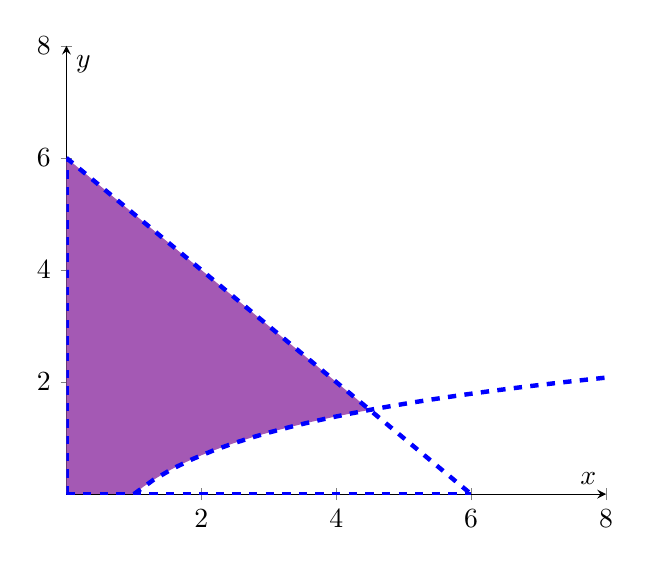
\begin{tikzpicture}[scale=1.0]
        \begin{axis}[
            axis x line=middle,
            axis y line=middle,
            ymin=0,ymax=8,ylabel=$y$,
            xmin=0,xmax=8,xlabel=$x$
        ]
            \begin{scope}
                \path[clip]
                    plot[domain=0:1] ({\x}, {0})
                    --plot[domain=1:4.49666] ({\x}, {ln(\x)})
                    --plot[domain=4.49666:0] ({\x}, {6-\x})
                    --plot[domain=0:6, variable=\y] ({0}, {\y})
                    --cycle;

                \fill [red!45!blue!65!] (0,0) rectangle (6,6);
            \end{scope}

            \plot[domain=0:6,blue,dashed,ultra thick] {6-\x};
            \plot[domain=1:8,blue,dashed,ultra thick] {ln(\x)};
            \plot[domain=0:6,blue,dashed,ultra thick] {0};
            \plot[domain=0:6,blue,dashed,ultra thick,variable=\y] ({0}, {\y});
        \end{axis}
    \end{tikzpicture}
\caption{Example feasible region (light purple) satisfying four constraints (dashed blue line)}
\label{fig:exmp-plant-feasible-region}
\end{figure}

\begin{exmp}
    Consider the problem of maximizing plant growth by manipulating quantities of two nutrients, $x_1$ and $x_2$. Let the plant height be $f(x_1, x_2) = 1 + x_1^2(x_2 - 1)^3e^{-x_1-x_2}$, with the constraints that $x_1 \geq 0$, $x_2 \geq 0$, $x_1 + x_2 \geq 6$, and $x_2 \geq \log x_1$. Then within the feasible region (depicted in Figure \ref{fig:exmp-plant-feasible-region}), $f$ is maximized by $(x_1, x_2) = (2, 4)$.
\end{exmp}

\begin{defn}
    For all $x \in \R^n$ and $\varepsilon > 0$, the \emph{$\varepsilon$-neighborhood} of $x$ is
    \[N_{\varepsilon}(x) = \left\{y \in \R^n \compbar \norm{x - y} < \varepsilon \right\}.\]
\end{defn}

\begin{exmp}
    In $\R^1$, $N_{3}(7)$ is $(4, 10)$.
\end{exmp}

\begin{defn}
    For any $S \subseteq \R^n$ and $x \in \R^n$, we say that $x$ is an \emph{interior point} of $S$ if there exists $N_{\varepsilon}(x) \subseteq S$. If every $N_{\varepsilon}(x)$ contains a point inside $S$ and a point not inside $S$, we say that $x$ is a \emph{boundary point} of $x$.
\end{defn}

\begin{defn}
    A set $S \subseteq \R^n$ is \emph{open} if every point in $S$ is an interior point of $S$, and \emph{closed} if $S$ contains every boundary point of $S$.
\end{defn}

\begin{exmp}
    In $\R^1$, any non-empty interval $[a, b]$ is closed, and non-empty $(a, b)$ is open.
\end{exmp}

\begin{exmp}
    Both $\emptyset$ and $\R^n \subseteq \R^n$ are both open and closed.
\end{exmp}

\begin{prop}
    Let $S \subseteq \R^n$. Then $S$ is open if and only if $\R^n - S$ is closed.
\end{prop}

\begin{proof}
    Assume that $S$ is open, and let $x$ be a boundary point of $\R^n - S$. Then for every $\varepsilon > 0$, by definition there exists $y, z \in N_{\varepsilon}(x)$ such that $y \in S$ and $z \in \R^n - S$. Therefore, $N_{\varepsilon}(x) \centernot\subseteq S$. It follows that $x \notin S$ by definition, and so $x \in \R^n - S$. Therefore, $\R^n - S$ contains every boundary point of itself, and so it is closed.

    Assume that $\R^n - S$ is closed, and let $x \in S$. Consider $N_{\varepsilon}(x)$. Since $\R^n - S$ contains all of its boundary points, $x$ cannot be a boundary point of $\R^n - S$, and so we know that there must be some $\varepsilon$ such that $N_{\varepsilon} \subseteq S$. Therefore, every $x \in S$ is an interior point of $S$, and so $S$ is closed by definition.
\end{proof}

\begin{exmp}
    We will examine a few cases in which minima and maxima may fail to first.

    \begin{itemize}
        \item Unbounded objective function, e.g. minimizing $\ln x$ such that $0 < x \leq 7$.
        \item Bounded objective function on open set, e.g. minimizing $\ln x$ such that $1 < x \leq 7$.
        \item Infeasible (feasible region is empty), e.g. minimizing $\ln x$ such that $1 < x$ and $x \leq 0.5$.
    \end{itemize}
\end{exmp}

\begin{exmp}
    When a solution exists, two distinct cases may occur.

    \begin{itemize}
        \item The solution is an interior point of the feasible region, e.g. minimizing $f(x) = 3 + (x - 2)^2$ such that $1 \leq x \leq 3$. The local minimum is $x^* = 2$, and $f'(x^*) = 0$.
        \item The solution is a boundary point of the feasible region, e.g. minimizing $f(x) = 3 + (x - 2)^2$ such that $x \leq 10$. Then $x^* = 10$, but $f'(x^*) \neq 0$.
    \end{itemize}
\end{exmp}

\begin{defn}
    Let $S \subseteq \R^n$ and $f: \R^n \to \R$. Consider $x^* \in S$. We say that $x^*$ is a \emph{global minimum} if for all $y \in S$, $f(x^*) \leq f(y)$, and a \emph{strict} global minimum if for all $y \in S - \{x^*\}$, $f(x^*) < f(y)$.
\end{defn}

\begin{defn}
    Let $S \subseteq \R^n$ and $f: \R^n \to \R$. Consider $x^* \in S$. We say that $x^*$ is a \emph{local minimum} if there exists an $\varepsilon$-neighborhood $N_{\varepsilon}(x^*)$ such that for all $y \in N_{\varepsilon}(x) \intersection S$, $f(x^*) \leq f(y)$, and a \emph{strict} local minimum if for all $y \in \left(N_{\varepsilon}(x) \intersection S\right) - \{x^*\}$, $f(x^*) < f(y)$.
\end{defn}

\begin{defn}
    Let $S \subseteq \R^n$ be a feasible region and $f: S \to \R$ an objective function. A \emph{stationary point} $x \in S$ is where $\nabla f(x) = \vec{0}.$
\end{defn}

\begin{rmk}
    Let $S \subseteq \R^n$, $x^*$ be an interior point of $S$, and $f: S \to \R$ be a sufficiently smooth continuous function. If $x^* \in S$ is a local minimum, then the \emph{gradient} of $f(x^*)$ is $\vec{0}$. However, $\nabla f(x^*) = \vec{0}$ does not imply that $x^*$ is a local minimum.
\end{rmk}

\subsection{Forms of Linear Programming Problems}

\begin{defn}
    A maximization or minimization linear programming problem in \emph{standard form} is a problem of the form:
    find $x \in \R^n$ that maximizes or minimizes $\transposeof{c}x$ such that $Ax = b$ and $x \geq \vec{0}$. The problem is said to be in \emph{canonical form} if the constraints are instead in the form $Ax \geq b$ (or $Ax \leq b$).
\end{defn}

\begin{exmp}
    Consider the problem of minimizing the cost per unit of chicken feed, while ensuring necessary nutrients are provided. Let $x_1, x_2, x_3, x_4$ denote the quantities of each of four ingredients, with cost per unit of $6.2$, $2.0$, $1.6$, and $3.2$ respectively. Let $n_1$, $n_2$, $n_3$ be the nutrients, with minimum required values of $6.2$, $11.9$, and $10.0$ respectively.

    \begin{minipage}{\linewidth}
        \begin{center}
        \captionof{table}{Nutrition values}
        \label{exmp-feed-nutrition-values}
        \begin{tabular}{c|cccc}
        & $x_1$ & $x_2$ & $x_3$ & $x_4$\\
        \hline
        $n_1$ & $1.2$ & $2.6$ & $0.0$ & $9.2$ \\ \hline
        $n_2$ & $3.9$ & $1.0$ & $0.8$ & $2.0$ \\ \hline
        $n_3$ & $6.0$ & $0.0$ & $4.0$ & $3.1$ \\
        \end{tabular}
        \end{center}
    \end{minipage}

    Let
    \[A = \begin{pmatrix}
        1.2 & 2.6 & 0.0 & 9.2 \\
        3.9 & 1.0 & 0.8 & 2.0 \\
        6.0 & 0.0 & 4.0 & 3.1
    \end{pmatrix},\; b = \begin{pmatrix}
        6.2 \\ 11.9 \\ 10.0
    \end{pmatrix},\; c = \begin{pmatrix}
        6.2 \\ 2.0 \\ 1.6 \\ 3.2
    \end{pmatrix},\; x = \begin{pmatrix}
        x_1 \\ x_2 \\ x_3 \\ x_4
    \end{pmatrix}\]
    then our problem is to minimize $\transposeof{c}x$ such that $Ax \geq b$ and $x \geq \vec{0}$. This form is the \emph{canonical form} of a linear programming problem.
\end{exmp}

\begin{rmk}
    We can easily convert problems expressed as a minimization problem into an equivalent maximization problem and vice versa, and between standard form and canonical form.
\end{rmk}

\begin{prop}
    Minimizing $\transposeof{c}x$ is equivalent to maximizing $-\transposeof{c}x$ (and so maximizing $\transposeof{c}x$ is equivalent to minimizing $-\transposeof{c}x$).
\end{prop}

\begin{proof}
    Let $P$ be a linear programming problem where we seek to minimize $\transposeof{c}x$, and let $S$ denote the feasible region of $P$. Now let $Q$ denote linear program where we seek to maximize $\transposeof{C}x$ that is otherwise identical to $P$. Let $x^{*}$ be a local minimum of $P$. By definition, there must exist some $\varepsilon$-neighborhood such that $\transposeof{c}x^{*} \leq \transposeof{c}y$ for all $y \in N_{\varepsilon}(x) \intersection S$. It follows that $-\transposeof{c}x^{*} \geq -\transposeof{c}y$ for all $y \in N_{\varepsilon}(x) \intersection S$, and so $x^{*}$ must be a local maximum of $Q$.
\end{proof}

\begin{prop}
    The constraint $Ax \geq b$ is equivalent to $-Ax \leq -b$, and $Ax \leq b$ is equivalent to $-Ax \geq -b$.
\end{prop}

\begin{prop}
    The constraint $Ax = b$ is equivalent to having both $Ax \geq b$ and $Ax \leq b$, and therefore is equivalent to $[A; -A] \geq [b; -b]$.
\end{prop}

\begin{prop}
    The constraint $Ax \geq b$ is equivalent to $Ax - z = b$, where $A \in M_{m \times n}(\R)$, $x \in \R^n$, and $z \in \R^m$ where $z \geq 0$. Here, $z$ is a vector of \emph{slack} variables.
\end{prop}

\begin{exmp}
    The constraints
    \begin{align*}
        a_{11}x_1 + a_{12}x_2 + a_{13}x_3 &\geq b_1 \\
        a_{21}x_1 + a_{22}x_2 + a_{23}x_3 &\geq b_2 \\
        a_{31}x_1 + a_{32}x_2 + a_{33}x_3 &\geq b_3 \\
        a_{41}x_1 + a_{42}x_2 + a_{43}x_3 &\geq b_4
    \end{align*}
    are equivalent to
    \begin{align*}
        a_{11}x_1 + a_{12}x_2 + a_{13}x_3 - x_4 &= b_1 \\
        a_{21}x_1 + a_{22}x_2 + a_{23}x_3 - x_5 &= b_2 \\
        a_{31}x_1 + a_{32}x_2 + a_{33}x_3 - x_6 &= b_3 \\
        a_{41}x_1 + a_{42}x_2 + a_{43}x_3 - x_7 &= b_4.
    \end{align*}
\end{exmp}

\begin{prop}
    We can incorporate the positivity constraints $x \geq 0$ into the general matrix constraints. The constraints $Ax \geq b$ and $x \geq 0$ are equivalent to \[\begin{bmatrix} A \\ I\end{bmatrix}x \geq \begin{bmatrix} b \\ 0 \end{bmatrix},\]
    and the constraints $Ax \leq b$ and $x \geq 0$ are equivalent to \[\begin{bmatrix} A \\ -I\end{bmatrix}x \leq \begin{bmatrix} b \\ 0 \end{bmatrix}.\]
\end{prop}

\begin{prop}
    We can transform an unconstrained problem into an equivalent problem with a positivity constraint.
\end{prop}

\begin{exmp}
    Consider the problem of minimizing $5x_1 + 6x_2$ such that $2x_1 - 3x_2 \geq 9$ and $x_1 + x_2 \geq -8$, with $x_1 \geq 0$ but $x_2$ unconstrained in sign. Define $x_2'$ and $x_2''$, and constrain $x_2', x_2'' \geq 0$. Let $x_2 = x_2' - x_2''$.
\end{exmp}

\begin{rmk}
    Constraints of the form $Ax = b$ are simply a system of equations, and therefore can be simplified using row operations by Theorem \ref{solutions-unchanged-by-row-ops}. Reduced row echelon form can help identified independent vs dependent variables.
\end{rmk}

\subsection{Polyhedrons}

\begin{defn}
    For non-zero $p \in \R^n$, the \emph{hyperplane} with normal vector $p$ is the orthogonal complement of $p$: \[\left\{x \in \R^n \compbar p \cdot x = 0 \right\},\]
    and the closed \emph{half-space} with normal vector $p$ is
    \[\left\{x \in \R^n \compbar p \cdot x \geq 0 \right\}.\]
    If we have $p \cdot x > 0$, we say it is an open half-space. We can replace $\geq$ and $>$ with $\leq$ and $<$ respectively.
\end{defn}

\begin{defn}
    A \emph{polyhedron} (or \emph{polyhedral set}) is the intersection of finitely many half spaces.
\end{defn}

\begin{defn}
    A polyhedron $P$ is \emph{bounded} if there exists $r \in \R$ such that $\norm{x} < r$ for all $x \in P$. A bounded polyhedron is known as a \emph{polytope}.
\end{defn}

\begin{prop}
    $P \subseteq \R^n$ is a polyhedron if and only if there exists $A \in M_{m \times n}(\R)$ and $b \in \R^m$ such that
    \[P = \left\{x \in \R^n \compbar Ax \geq b\right\}.\]
\end{prop}

\begin{defn}
    Let $X = \{x_1, \ldots, x_k\} \subset \R^n$. A \emph{convex combination} of $X$ is
    \[\lambda_1 x_1 + \lambda_2 x_2 + \cdots + \lambda_k x_k,\]
    where $\lambda_i \geq 0 \in \R$ and $\sum_{i=1}^{k}\lambda_i = 1$.
\end{defn}

\begin{defn}
    A set $S \subseteq \R^n$ is \emph{convex} if for any $x, y \in S$ and convex combination $z$ of $x$ and $y$, then $z \in S$.
\end{defn}

\begin{thm}
    Every polyhedron is convex.
\end{thm}

\begin{proof}
    Let $P = \left\{x \in \R^n, \compbar Ax \geq b\right\}$ be a polyhedron in $\R^n$. Let $x, y \in P$ and $z = \lambda x + (1 - \lambda) y$ be a convex combination of $x$ and $y$ for some $\lambda \in [0, 1]$.

    We know that $Ax \geq b$ and $Ay \geq b$, and want to show that $Az \geq b$. Since $z = \lambda x + (1 - \lambda)y$,
    \begin{align*}
        Az = A\left(\lambda x + (1 - \lambda)y\right) = \lambda Ax + (1 - \lambda)Ay \geq \lambda b + (1 - \lambda) b = b,
    \end{align*}
    and so $Az \geq b$.
\end{proof}

\begin{thm}
    A set $S \subseteq \R^n$ is convex if and only if every convex combination of every finite $X \subseteq S$ is in $S$.
\end{thm}

\begin{proof}
    We will prove this by showing that this is equivalent to the definition.
    
    $(\impliedby)$ If every convex combination of finite $X \subseteq S$ is in $S$, then every convex combination of $x, y \in S$ is in $X$.

    $(\implies)$ We will prove, via induction on $n = \abs{X}$, that if $z$ is a convex combination of $x, y \in S$ implies that $z \in S$, then every convex combination of $X \subseteq S$ is also in $S$.

    First, consider the base case of $n=1$, so $X = \{x\} \subseteq S$. The only convex combination of $X$ is simply $x$, and so every convex combination of $X$ is in $S$. Next, assume that if $z$ is a convex combination of $x, y \in S$ implies that $z \in S$, then every convex combination of $X \in S$ where $\abs{X} = n$ is also in $S$. For any $X' \subseteq S$ where $\abs{X'} = n+1$, there is some $X \subsetneq X'$ such that $\abs{X} = n$. Then every convex combination of $X$ is in $S$. Let \[\lambda_1x_1 + \cdots + \lambda_n x_n + \lambda_{n+1}x_{n+1}\] be a convex combination of $X$. Let $\Lambda = \lambda_1 + \cdots + \lambda_n$, and note that
    \[\alpha = \frac{\lambda_1}{\Lambda}x_1 + \cdots + \frac{\lambda_n}{\Lambda}x_n\] is a convex combination of $X$ and so must be in $S$ by by the induction hypothesis. Furthermore, note that
    \[\Lambda \alpha + \lambda_{n+1}x_{n+1}\] is our original convex combination of $X'$, but is also a convex combination of two points in $S$, and so is also in $S$ by assumption.
\end{proof}

\begin{defn}
    Let $S$ be a convex set, and consider $x \in S$. If $x$ being a convex combination of $y, z \in S$ implies that $x = y = z$, we say that $x$ is an \emph{extreme point}.
\end{defn}

\subsection{Basic Feasible Solutions}

\begin{defn}
    Let $c \in \R^n$, $A \in M_{m \times n}(\R)$, and $b \in \R^m$ be the linear program with feasibility region \[S = \left\{x \in \R^n \compbar Ax = b, x \geq \vec{0}\right\}.\] Let $A$ have rank $m$, or else eliminate redundant constraints until it does.

    Let $B$ be a subset of $m$ of the indices $\{1, \ldots, n\}$ such that the corresponding columns of $A$ form a basis for the column space of $A$ (which is $\R^m$ since $A$ has rank $m$). Let $A_B \in M_{m \times m}(\R)$ denote the invertible matrix of these columns.

    A \emph{basic feasible solution} is any $x \in S$ where $j \notin B$ implies $x_j = 0$.
\end{defn}

\begin{rmk}
    Without loss of generality, we can rearrange the columns of $A$ such that $A = [A_B | N]$, and then basic feasible solutions are precisely those $x \in S$ such that $x = \begin{bmatrix}
        x_B \\ x_N
    \end{bmatrix}$ where $x_N = \vec{0}$.
\end{rmk}

\begin{thm}
    Let $B \in M_{m \times m}(\R)$ have rank $m$, and $N \in M_{m \times (n-m)}(\R)$ where $m < n$, and then let $A = [B | N] \in M_{m \times n}(\R)$. Let $b \in \R^m$, so the feasible region is \[S = \left\{x \in \R^n \compbar Ax = b,\; x \geq \vec{0}\right\}.\]

    Then $x \in S$ is an extreme point of $S$ if and only if $x$ is a basic feasible solution of $S$.
\end{thm}

\begin{proof}\proofbreak
    ($\impliedby$) Suppose $x$ is a basic feasible solution of $S$, so $x = \begin{bmatrix}
        x_B \\ x_N
    \end{bmatrix}$ where $x_N = \vec{0}$. Let $x = \lambda x' + (1 - \lambda) x''$ be a non-trivial convex combination (so $0 < \lambda < 1$) of $x', x'' \in S$. We can represent $x'$ and $x''$ as $x' = \begin{bmatrix} x_B' \\ x_N' \end{bmatrix}$ and $x'' = \begin{bmatrix} x_B'' \\ x_N'' \end{bmatrix}$ respectively. Notice that we now have $x_N = \vec{0} = \lambda x_N' + (1 - \lambda)x_N''$. Since $x', x'' \in S$, we know $x_N', x_N'' \geq 0$ and so we necessarily have $x_N' = x_N'' = 0$. But then $x'$ and $x''$ are also basic feasible solutions. Since $A_{B}$ is invertible and $x, x', x'' \in S$, we know that $A_{B}x_B = A_{B}x_B'b = A_{B}x_B''$, and so $x = x' = x''$.

    ($\implies$) Suppose $x$ is not a basic feasible solution of $S$. Then $x = \begin{bmatrix}
        x_B \\ x_N
    \end{bmatrix}$ where $x_N$ is nonzero. We know that the columns of $A$ corresponding to the non-zero entries of $x$ must be linearly dependent, or else we can complete them to a basis for $\R^m$ and $x$ would be a basic feasible solution. Therefore, we know there exists non-zero $z$ such that $Az = \vec{0}$ and $z_i \neq 0$ implies $x_i \neq 0$. Note that for any $\alpha \in \R$, $A(x + \alpha z) = Ax + \alpha Az = b$, so any $x + \alpha z \geq \vec{0}$ is a feasible solution. Since $x_i$ is strictly greater than zero when $z_i \neq 0$, for sufficiently small $\varepsilon$ the points $x + \varepsilon z$ and $x - \varepsilon z$ must be feasible. Then $x = \frac{1}{2}\left(x + \varepsilon z\right) + \left(1 - \frac{1}{2}\right)\left(x - \varepsilon z\right)$, and so $x$ can be expressed as a non-trivial convex combination in $S$ and therefore is not extreme.
\end{proof}

\subsection{Simplex Method}

\begin{defn}
    Consider a linear program in standard form. Given a choice of basis $B$ such that $A = [B | N]$, the \emph{pre-tableau} is the matrix
    \begin{align*}
        \left[\begin{array}{c|c|c|c}
            1 & -\transposeof{c_B} & -\transposeof{c_N} & 0 \\
            \hline
            \vec{0} & B & N & b
        \end{array}\right].
    \end{align*}
    In other words, we have augment $A = [B|N]$ with the constraint values $b$, and then again with a new variable $z$ in the first column/row such that $z - \transposeof{c}x = 0$. Note that $z$ is therefore the value of the objective function.
\end{defn}

\begin{defn}
    Given a linear program in standard form, and basic feasible solution $\transposeof{x} = [\transposeof{x_B}, \vec{0}]$, the corresponding \emph{basic feasible simplex tableau} is the matrix
    \begin{align*}
        \left[\begin{array}{c|c|c|c}
            1 & 0 & \transposeof{c_B}B^{-1}N-\transposeof{c_N} & \transposeof{c_B}B^{-1}b \\
            \hline
            \vec{0} & I & B^{-1}N & B^{-1}b
        \end{array}\right].
    \end{align*}
\end{defn}

\begin{rmk}
    The basic feasible tableau is the reduced row echelon form of the pre-tableau. It can also be obtain by left-multiplying the pre-tableau by
    \begin{align*}
        \left[\begin{array}{c|c}
            1 & \transposeof{c_B}B^{-1} \\
            \hline
            \transposeof{\vec{0}} & B^{-1}
        \end{array}\right].
    \end{align*}
\end{rmk}

\begin{rmk}
    We can see that $z + (\transposeof{c_B}B^{-1}N-\transposeof{c_N})x_N = \transposeof{c_B}B^{-1}b$, so $z = \transposeof{c_B}B^{-1}b + (\transposeof{c_N} - \transposeof{c_B}B^{-1}N)x_N$. We often denote this as
    \[z = \transposeof{c_B}B^{-1}b + \transposeof{r_N}x_N,\]
    where
    \[\transposeof{r_N} = \transposeof{c_N} - \transposeof{c_B}B^{-1}N.\]
\end{rmk}

In the simplex, we start with a linear program $A, b, c$ in standard form. Assuming we already know a basis that leads to a basic feasible solution, we form the pre-tableau and either row-reduce or multiply through by the matrix from the above remark to obtain the basis feasible tableau.

To illustrate the linear program, we will consider
\begin{align*}
    A =
    \begin{bmatrix}
        2 & -1 & 3 & 7 & 1 & 2 & 8 \\
        5 & 2 & -8 & -1 & 2 & 0 & 1 \\
        4 & 6 & -2 & 4 & 1 & 3 & -5
    \end{bmatrix},\;\;
    b = \begin{bmatrix}
        2 \\ 4 \\ 3
    \end{bmatrix},\;\;
    \transposeof{c} = [6, -3, 2, 1, -1, 7, 1].
\end{align*}

We will use columns $1$, $3$, and $7$ as our basis columns, however we will leave the columns in their original order to make bookkeeping easier. Our pre-tableau is
\begin{align*}
    \left[\begin{array}{c|ccccccc|c}
        1 & -6 & 3 & -2 & -1 & 1 & -7 & -1 & 0 \\
        \hline
        0 & 2 & -1 & 3 & 7 & 1 & 2 & 8 & 2 \\
        0 & 5 & 2 & -8 & -1 & 2 & 0 & 1 & 4 \\
        0 & 4 & 6 & -2 & 4 & 1 & 3 & -5 & 3
    \end{array}\right].
\end{align*}

Row-reducing to the reduced row echelon form (while treating columns $1$, $3$, and $7$ as leading columns) brings us to our first basic feasible tableau:
\begin{align*}
    \left[\begin{array}{c|ccccccc|c}
        1 & 0 & 9.35 & 0 & 11.06 & 2.82 & -1.22 & 0 & 4.93 \\
        \hline
        0 & 1 & 1.03 & 0 & 1.62 & 0.31 & 0.82 & 0 & 0.81 \\
        0 & 0 & 0.33 & 1 & 1.14 & -0.05 & 0.50 & 0 & 0.01 \\
        0 & 0 & -0.51 & 0 & 0.04 & 0.07 & -0.14 & 1 & 0.04
    \end{array}\right].
\end{align*}

Now, we \emph{pivot} to a new (and improved!) basic feasible tableau by choosing a non-basis column to turn into a basis column. We make the greediest choice by choose the $4$th column ($5$th of the overall tableau) since it has the largest improvement to our objective function per unit change in the corresponding non-basis variable.

Letting $j = 4$, we choose the $k$th row (excluding the objective row on top) by \[\argmin_{k}\frac{b_k}{A_{kj}} \mathrm{ where } A_{kj} > 0.\] This gives us the $2$nd row, so we row-reduce again, replace the column whose leading term choose in the $2$nd row (which is column $3$) with column $4$. To do this, we treat column $4$ as if it was the second column while row-reducing. Our new basis columns are $1$, $4$, and $7$, giving us our second basic feasible tableau:
\begin{align*}
    \left[\begin{array}{c|ccccccc|c}
        1 & 0 & 6.14  & -9.67 & 0 & 3.29  & -6.01 & 0 & 4.81 \\
        \hline
        0 & 1 & 0.56  & -1.41 & 0 & 0.37  & 0.11  & 0 & 0.79 \\
        0 & 0 & 0.28  & 0.87  & 1 & -0.04 & 0.43  & 0 & 0.01 \\
        0 & 0 & -0.57 & -0.03 & 0 & 0.06  & -0.15 & 1 & 0.04
    \end{array}\right].
\end{align*}

Note that the objective function value has decreased from $4.93$ to $4.81$. We now continue pivoting in the manner, the objective function value decreasing from $4.81$, to $4.6$, to $-2.45$, to $-2.46$. When there are no positive entries in the objective function row (top row), there are no more improvements that can be made by changing our choice of basis and we have reached optimality.

\subsection{Two-Phase Method}

The Two-Phase Method is a technique for coming up with the initial basic feasible solution need to start off the Simplex Method. In Phase I, we solve a different linear program to find the initial basic feasible solution, and then in Phase II we use that basic feasible solution to apply the simplex method to the original linear program. We take a problem in standard form with constraints $Ax = b$, $x \geq 0$ where $A \in M_{m \times n}(\R)$. We then introduce \emph{artificial variables} $x_{n+1}, x_{n+2}, \ldots, x_{n+m}$ for each constraint (row) in $A$. Let $x'$ denote the vector obtained by appending the artificial variables to $x$.

For Phase I, we solve a different problem using the Simplex Method: minimizing $x_{n+1} + x_{n+2} + \cdots + x_{n+m}$ such that $[A|I]x' = b$, $x' \geq 0$. Notice that any feasible solution to this new problem is a feasible solution to the original linear program if the objective function value is zero. Therefore, the $x$ part of an optimal solution $x'$ to the new problem is a feasible solution to the original if $x'$ has objective function value zero. If the optimal solution $x'$ has a positive objective function value, then no feasible solution exists for the original linear program.

Note that
\begin{align*}
    x' = \begin{bmatrix}
        x \\
        x_{n+1} \\
        \vdots \\
        v_{n+m}
    \end{bmatrix} = \begin{bmatrix}
        0 \\
        b_1 \\
        \vdots \\
        b_m
    \end{bmatrix}
\end{align*}
is always a basic feasible solution to the Phase I problem. Therefore, we can immediately apply the Simplex method to determine the feasibility of the original linear program, and find a feasible solution if one exists. Additionally, since the number of columns in a basis for either linear program is the same (always just $m$), the feasible solution given to us by Phase I must in fact be a basic feasible solution for Phase II.

\subsection{Big-M Method}

In the Big-M method, we essentially combine the two phases of the Two-Phase method by using the objective function
\begin{align*}
    \transposeof{c}x + M(x_{n+1} + x_{n+2} + \cdots + x_{n+m}),
\end{align*}
where $M$ is a very large value. This penalizes the artificial variables and causes them to be zero in any optimal solution. Setting the artificial variables to $b$ gives us an initial basic feasible solution. If a basic feasible solution exists where the artificial variables are zero, the first $m$ pivots will replace each artificial variable with non-artificial variables, and so the final optimal solution will be a solution to the original linear program.

\subsection{Duality}

\begin{defn}{Canonical or symmetric duality}\proofbreak
    Consider a linear program of the form minimize $\transposeof{c}x$ such that $Ax \geq b$ and $x \geq \vec{0}$. The \emph{dual} problem is maximizing $\transposeof{b}y$ such that $\transposeof{A}y \leq c$ and $y \geq \vec{0}$. The original linear program is referred to as the \emph{primal} probem in relation to its dual.
\end{defn}

\begin{exmp}
    Consider minimizing $1x_1 + 2x_2$ such that
    \begin{align*}
        3x_1 + 4x_2 &\geq 9, \\
        5x_1 + 6x_2 &\geq 10, \\
        7x_1 + 8x_2 &\geq 11, \\
        x_1, x_2 &\geq 0.
    \end{align*}

    The dual problem is maximizing $9y_1 + 10y_2 + 11y_3$ such that
    \begin{align*}
        3y_1 + 5y_2 + 7y_3  &\leq 1, \\
        4y_1 + 6y_2 + 8y_3  &\leq 2, \\
        y_1, y_2, y_3 &\geq 0.
    \end{align*}
\end{exmp}

\begin{defn}{Standard duality}\proofbreak
    Consider a linear program of the form minimization of $\transposeof{c}x$ such that $Ax = b$ and $x \geq \vec{0}$. The \emph{dual} problem is maximizing $\transposeof{b}y$ such that $\transposeof{A}y \leq c$, \emph{without} a non-negativity constraint on $y$. The original linear program is again referred to as the \emph{primal} probem in relation to its dual.
\end{defn}

\begin{rmk}
    We can derive the canonical form of duality from the standard form, and vice versa. Imagine we know that the dual of minimizing $\transposeof{c}x$ such that $Ax = b$ and $x \geq \vec{0}$ was to maximize $\transposeof{b}y$ such that $\transposeof{A}y \leq c$. If we were now given a linear program in canonical form and wanted to find its dual, we could first convert it into standard form by the introduction of slack variables, obtaining minimize $\transposeof{c}x$ such that $[A|-I]\begin{bmatrix}x \\ z\end{bmatrix} = b$ such that $\begin{bmatrix}x \\ z\end{bmatrix} \geq 0$. The standard dual of this is to maximize $\transposeof{b}y$ such that $\transposeof{[A|-I]}y \leq \begin{bmatrix}c \\ \vec{0}\end{bmatrix}$, which is equivalent to maximizing $\transposeof{b}y$ such that $\transposeof{A}y \leq c$ and $y \geq \vec{0}$ (from $-y \leq \vec{0}$).
\end{rmk}

\begin{prop}
    The canonical and standard duals of equivalent linear programs are equivalent.
\end{prop}

\begin{proof}
    See figure \ref{fig:duality-equivalence}.
\end{proof}

\begin{figure}[ht]
    \centering
    \begin{tikzpicture}[{baseline=(current bounding box.north)}]
        \node[align=center] at (-3,2.5) {$
            \begin{aligned}
                \mathrm{min.}\;\transposeof{c}&x \\
                \mathrm{s.t.}\;A&x \geq b, \\
                        &x \geq \vec{0}.
            \end{aligned}
        $};
        \node[align=center] at (3,2.5) {$
            \begin{aligned}
                \mathrm{max.}\;\transposeof{b}&y \\
                \mathrm{s.t.}\;\transposeof{A}&y \leq c, \\
                        &y \geq \vec{0}.
            \end{aligned}
        $};
        \node[align=center] at (-3,-3) {$
            \begin{aligned}
                \mathrm{min.}\;\transposeof{\begin{bmatrix}c \\ \vec{0}\end{bmatrix}}&\begin{bmatrix}x \\ z\end{bmatrix} \\
                \mathrm{s.t.}\;\left[A|-I\right]&\begin{bmatrix}x \\ z\end{bmatrix} = b, \\
                        &x, z \geq \vec{0}.
            \end{aligned}
        $};
        \node[align=center] at (3,-3) {$
            \begin{aligned}
                \mathrm{max.}\;&\transposeof{b}y \\
                \mathrm{s.t.}\;&\begin{bmatrix}\transposeof{A} \\ -I\end{bmatrix}y \leq \begin{bmatrix}c \\ \vec{0}\end{bmatrix}.
            \end{aligned}
        $};

        \draw[ultra thick, blue, ->] (-1, 3) -- (1, 3);
        \draw[ultra thick, red, ->] (-1, -3) -- (1, -3);
        \draw[ultra thick, black, <->] (3, -1) -- (3, 1);
        \draw[ultra thick, black, <->] (-3, 1) -- (-3, -1);

    \end{tikzpicture}
\caption{Equivalence of dualities}
\label{fig:duality-equivalence}
\end{figure}

\newpage

\begin{prop}
    Given a primal linear program, the dual of the dual is the primal.
\end{prop} 

\begin{proof}
    Consider a linear program in canonical form.  By definition, the dual is maximizing $\transposeof{b}y$ such that $\transposeof{A}y \leq c$ and $y \geq 0$. This program is equivalent to minimizing $-\transposeof{b}y$ such that $-\transposeof{A}y \geq -c$ and $y \geq 0$. The dual of this equivalent form of the dual is to maximizing $-\transposeof{c}x$ such that $\transposeof{\left(-\transposeof{A}\right)}x \leq -b$ and $x \geq 0$. Finally, this program is equivalent to minimizing $\transposeof{c}x$ such that $Ax \geq b$ and $x \geq 0$, which is the primal linear program.
\end{proof}

\begin{thm}{Weak Duality}\label{weak-duality}\proofbreak
    Consider a linear program and its dual, and $x, y$ feasible solutions to the primal and dual programs respectively. Then the objective function value at $y$ in the dual is less than or equal to the objective function value at $x$ in the primal.
\end{thm}

\begin{proof}
    When the primal is in standard form, we have $Ax = b$, $x \geq \vec{0}$ and $\transposeof{A}y \leq c$. It follows that $\transposeof{b}y = \transposeof{(Ax)}y = \transposeof{x}\transposeof{A}y$. Since we have $x \geq \vec{0}$, we know that $\transposeof{x}\transposeof{A}y \leq \transposeof{x}c$, and so $\transposeof{b}y \leq \transposeof{c}x$.

    When the primal is in canonical form, we have $Ax \geq b$, $x \geq \vec{0}$, $\transposeof{A}y \leq c$, and $y \geq 0$. Since $y \geq \vec{0}$, $Ax \geq b$ implies that $\transposeof{b}y \leq \transposeof{(Ax)}y$, and so $\transposeof{b}y \leq \transposeof{x}\transposeof{A}y$. Furthermore, since $\transposeof{A}y \leq c$ and $x \geq \vec{0}$, $\transposeof{x}\transposeof{A}y \leq \transposeof{x}c = \transposeof{c}x$. Combining these, we arrive at $\transposeof{b}y \leq \transposeof{c}y$.
\end{proof}

\begin{cor}
    The optimal objective value function in the dual is less than or equal to the optimal objective function value in the primal.
\end{cor}

\begin{cor}{Supervisor principle}\label{supervisor-principle}\proofbreak
    If $\transposeof{b}y = \transposeof{c}x$, then $x$ and $y$ are optimal in their respective linear programs.
\end{cor}

\begin{thm}{Strong Duality}\label{strong-duality}\proofbreak
    Suppose a linear program has a feasible solution and its objective function is bounded from below. Then the linear program and its dual have optimal solutions $x$ and $y$ respectively, and the objective function value of $x$ and $y$ are equal.
\end{thm}

\begin{proof}
    Consider the primal in standard form. We can apply the Simplex method or similar to obtain an optimal basic feasible solution $x^*$. Without loss of generality, we can assume that the final basis consists of the first $m$ columns of $A$.

    By the terminating condition of the Simplex method, we know that
    \begin{align*}
        \transposeof{r_N} = \transposeof{c_N} - \transposeof{c_B}B^{-1}N \geq \vec{0}.
    \end{align*}
    Let
    \begin{align*}
        \transposeof{y^*} = \transposeof{c_B}B^{-1}.
    \end{align*}

    Since $\transposeof{r_N} \geq \vec{0}$, we know that
    \begin{align*}
        \transposeof{c_B}B^{-1}N \leq \transposeof{c_N},
    \end{align*}
    and so it follows that
    \begin{align*}
        \transposeof{y^*}A = \transposeof{c_B}B^{-1}[B|N] = [\transposeof{c_B}|\transposeof{c_B}B^{-1}N] \leq [\transposeof{c_B}|\transposeof{c_N}] = \transposeof{c},
    \end{align*}
    so $y^*$ is a feasible solution to the dual. Now we can show that the objective function values are equal:
    \begin{align*}
        \transposeof{y^*}b = \transposeof{c_B}B^{-1}b = \transposeof{\begin{bmatrix}c_B \\ \vec{0}\end{bmatrix}}\begin{bmatrix}x_B \\ \vec{0}\end{bmatrix} = \transposeof{c}x^*.
    \end{align*}

    Therefore, $y^*$ is an optimal solution to the dual linear program by the supervisor principle \ref{supervisor-principle}.
\end{proof}

\subsection{Sensitivity Analysis}

\begin{defn}
    A basic feasible solution $b$ to a linear program with basis $B$ is \emph{non-degenerate} when $B^{-1}b > \vec{0}$.
\end{defn}

Consider solving a linear program $A, b, c$ in standard form by the Simplex method. What happens if we replace $b$ with $b' = b + \Delta b$ for some arbitrary $\Delta b$? If we replaced $B^{-1}b$ with $B^{-1}(b + \Delta b)$ and $\transposeof{c_B}B^{-1}b$ with $\transposeof{c_B}B^{-1}(b + \Delta b)$ in just the final basic feasible simplex tableau, what happens?

If $B^{-1}(b + \Delta b) \geq \vec{0}$, then we still have a basic feasible solution! Furthermore, since the objective row would still be non-positive, our solution would also be an \emph{optimal} basic feasible solution. This would very likely only occur when $\Delta b$ is fairly small.

If the linear program is non-degenerate, there always exists such $\Delta b$ small enough.

In the corresponding dual linear program, we know that
\begin{align*}
    \transposeof{y^*} = \transposeof{c_B}B^{-1}.
\end{align*}
We also have $\transposeof{c}x^* = \transposeof{y^*}b$, and so when we replace $b$ with $b'$ we get
$\transposeof{c}{x'}^{*} = \transposeof{y^*}(b + \Delta b) = \transposeof{y^*}b + \transposeof{y^*}\Delta b$. Therefore,
\begin{align*}
    \frac{\transposeof{c}{x'}^{*}}{\partial b_i} = y_i^*.
\end{align*}

\begin{defn}
    Vectors $x, y \in \R^n$ are \emph{complementary} if $x_i \neq 0 \implies y_i = 0$ and $y_i \neq 0 \implies x_i = 0$.
\end{defn}

\begin{prop}\label{complementary-orthogonal}
    If $x \geq 0$ and $y \geq 0$, then $x$ and $y$ are complementary if and only if $\transposeof{x}y = 0$.
\end{prop}

\begin{proof}
    If $x$ and $y$ are complementary, then $x_iy_i = 0$, and so $\transposeof{x}y = 0$.

    Since $x \geq 0$ and $y \geq 0$, we know $x_iy_i \geq 0$. If $\transposeof{x}y = 0$, then we must have $x_iy_i = 0$. Therefore at least one of $x_i$ and $y_i$ is zero and so $x$ and $y$ are complementary.
\end{proof}

\begin{thm}{Complementary slackness}\label{complementary-slackness}\proofbreak
    Consider a linear program $A, b, c$ in standard form. Let $x \in \R^n$ be a feasible solution. Let $y \in \R^m$ be a feasible solution in the dual. Then $x$ and $y$ are optimal solutions if and only if $c - \transposeof{A}y$ is complentary to $x$.
\end{thm}

\begin{proof}
    Recall that
    \begin{align*}
        \transposeof{b}y = \transposeof{(Ax)}y = \transposeof{x}\transposeof{A}y \leq \transposeof{x}c = \transposeof{c}x.
    \end{align*}
    By the supervisor principle \ref{supervisor-principle}, $x$ and $y$ are optimal if and only if $\transposeof{b}y = \transposeof{c}x$, which is equivalent to $\transposeof{x}\transposeof{A}y = \transposeof{x}c$. Therefore,
    \begin{align*}
        \transposeof{x}\left(c - \transposeof{A}y\right) = \vec{0}.
    \end{align*}

    Since $y$ is feasible in the dual, by definition $\transposeof{A}y \leq c$, and so $c - \transposeof{A}y \geq \vec{0}$. Furthermore, $x \geq 0$ and so by Proposition \ref{complementary-orthogonal} it follows that this occurs precisely when $x$ and $c - \transposeof{A}y$ are complementary.
\end{proof}

\subsection{Dual Simplex Method}

In the dual simplex method, we have a linear program in standard form. Unlike when we start the simplex method, rather than knowing a starting feasible solution and working towards optimality, we know a starting solution that is essentially optimal and works towards feasibility. We actually start with a vector $y$ that is feasible in the dual linear program, and work towards making the corresponding primal vector $x$ feasible in the primal. Due to the setup of the dual simplex method, both $y$ and $x$ will have the same objective function value, and so once $x$ is feasible we have an optimal solution by the supervisor principle \ref{supervisor-principle}.

\begin{defn}{Basic tableau}\proofbreak
    A basic tableau is a tableau formed from a basic, but not necessarily feasible, solution.
\end{defn}

Given a linear program in standard form and corresponding basic tableau, we have $\transposeof{y} = \transposeof{c_B}B^{-1}$ and $x = B^{-1}b$. Recall that $y$ is an optimal solution to the dual problem when:
\begin{itemize}
    \item $Ax = b$,
    \item $x \geq 0$,
    \item $\transposeof{A}y \leq c$,
    \item $\transposeof{c}x = \transposeof{b}y$.
\end{itemize}

The first condition, that $Ax = b$ is necessarily satisfied by any basic tableau. The fourth, that $\transposeof{c}x = \transposeof{b}y$, is also satisfied since $\transposeof{c_B}B^{-1}b = \transposeof{y}b = \transposeof{b}y$ and $\transposeof{c_B}B^{-1}b = \transposeof{c}x$. The third condition, that $\transposeof{A}y \leq c$, is satisfied when $r \geq 0$. Since the top row of the tableau is $-r$, to have dual feasibility at the start of the dual simplex method we require that $-r \leq 0$ --- that is, that the top row of the basic tableau is non-positive other than the constant $1$. Therefore, we need to come up with a ``dual pivot'' that preserves these properties while working towards achieving the second condition.

To dual pivot, we choose the row $j$ with the most-negative value in $B^{-1}b$, and pick a column to row-reduce on. Since we need to maintain a non-positive top row $-r$, we want to pick the column $k$ by \[\argmin_{k}\frac{r_k}{A_{jk}} \mathrm{ where } A_{jk} < 0.\]

\section{Non-Linear Programming}

\begin{defn}
    Let $S \subseteq \R^n$ be a non-empty convex set, and let $f: S \to \R$. We say that $f$ is \emph{convex} when
    \begin{align*}
        f\left(\lambda x + (1 - \lambda)y\right) \leq \lambda f(x) + (1 - \lambda)f(y)
    \end{align*}
    for all $x, y \in S$ and $\lambda \in [0, 1]$.

    Similarly, we say that $f$ is \emph{strictly convex} when
    \begin{align*}
        f\left(\lambda x + (1 - \lambda)y\right) < \lambda f(x) + (1 - \lambda)f(y)
    \end{align*}
    for all $x, y \in S$ and $\lambda \in (0, 1)$.

    We analogously define \emph{concave} and \emph{strictly concave} functions using $\geq$ and $>$ respectively.
\end{defn}

\begin{rmk}
    Note that we use an open interval for $\lambda$ in the strict case, and a closed interval otherwise. This is because at $\lambda = 0$ or $\lambda = 1$ we will always have equality.
\end{rmk}

\begin{defn}
    Let $S \subseteq \R^n$, and consider $f: S \to \R$. The \emph{epigraph} of $f$ 
    \begin{align*}
        \left\{\begin{bmatrix}
            x \\ y
        \end{bmatrix} \compbar x \in S, y \in R, y \geq f(x)\right\} \subseteq \R^{n+1}
    \end{align*}
    and is denoted by $\epigraph(f)$. That is, the epigraph is all points above the graph of the function.
\end{defn}

\begin{prop}\label{epigraph-convexity}
    Let $S \subseteq \R^n$, and consider $f: S \to \R$. Then $f$ is a convex function if and only if $\epigraph(f)$ is a convex set.
\end{prop}

\begin{proof}\proofbreak
    ($\implies$) Assume that $f$ is convex. Then for any $\transposeof{[x_1, y_1]}, \transposeof{[x_2, y_2]} \in \epigraph(f)$ and $\lambda \in [0, 1]$, we know that
    \begin{align*}
        f(\lambda x_1 + (1 - \lambda)x_2) \leq \lambda f(x_1) + (1 - \lambda)f(x_2) \leq \lambda y_1 + (1 - \lambda)y_2.
    \end{align*}
    Therefore,
    \begin{align*}
        \lambda \begin{bmatrix}
            x_1 \\ y_1
        \end{bmatrix} + (1-\lambda)\begin{bmatrix}
            x_2 \\ y_2
        \end{bmatrix} = \begin{bmatrix}
            \lambda x_1 + (1 - \lambda)x_2 \\
            \lambda y_1 + (1 - \lambda)y_2
        \end{bmatrix} \in \epigraph(f),
    \end{align*}
    and so $\epigraph(f)$ is a convex set.

    ($\impliedby$) Assume that $\epigraph(f)$ is a convex set. Since we trivially have $f(x) \leq f(x)$ for all $x \in S$, we know that for any $x_1, x_2 \in S$ we have
    \begin{align*}
        \transposeof{[x_1, f(x_1)]}, \transposeof{[x_2, f(x_2)]} \in \epigraph(f).
    \end{align*}
    Since $\epigraph(f)$ is convex, for all $\lambda \in [0, 1]$ we also know that
    \begin{align*}
        \lambda \begin{bmatrix}
            x_1 \\ f(x_1)
        \end{bmatrix} + (1-\lambda)\begin{bmatrix}
            x_2 \\ f(x_2)
        \end{bmatrix} = \begin{bmatrix}
            \lambda x_1 + (1 - \lambda)x_2 \\
            \lambda f(x_1) + (1 - \lambda)f(x_2)
        \end{bmatrix} \in \epigraph(f).
    \end{align*}
    Therefore,
    \begin{align*}
        f(\lambda x_1 + (1 - \lambda)x_2) \leq \lambda f(x_1) + (1-\lambda)f(x_2)
    \end{align*}
    by the definition of $\epigraph(f)$, and so $f$ is a convex function.
\end{proof}

\begin{thm}{Support Theorem}\label{support-theorem}\proofbreak
    Let $S \subseteq \R^n$ be a convex set, and let $\bar{x}$ be a boundary point of $S$. There exists a hyperplane containing $\bar{x}$ such that $S$ is contained in an associated closed half-space.
\end{thm}

\begin{thm}\label{convex-function-tangent-hyperplane}
    Let $S \subseteq \R^n$ be an open convex set, and let $f: S \to \R$ be continuously differentiable. Then $f$ is a convex function if and only if
    \begin{align*}
        f(x) \geq f(\bar{x}) + \transposeof{\nabla f(\bar{x})}(x - \bar{x})
    \end{align*}
    for all $x, \bar{x} \in S$. 
\end{thm}

\begin{thm}
    Let $S \subseteq \R^n$ be an open convex set, and let $f: S \to \R$ be continuously differentiable. Then $f$ is strictly convex if and only if 
    \begin{align*}
        f(x) > f(\bar{x}) + \transposeof{\nabla f(\bar{x})}(x - \bar{x})
    \end{align*}
    for all $x, \bar{x} \in S$ where $x \neq \bar{x}$. 
\end{thm}

\begin{cor}
    Let $S \subseteq \R^n$ be an open convex set, and let $f: S \to \R$ be \emph{twice} continuously differentiable. Then $f$ is convex if and only if $\nabla^2f(\bar{x})$ is positive semi-definite for all $\bar{x} \in S$.
\end{cor}

\begin{proof}\proofbreak
    Assume $\nabla^2f(\bar{x})$ is positive semi-definite for all $\bar{x} \in S$. By Taylor's theorem, for all $x \in S$ we have
    \begin{align*}
        f(x) = f(\bar{x}) + \transposeof{\nabla f(\bar{x})}(x - \bar{x}) + \frac{1}{2}\transposeof{(x - \bar{x})}\nabla^2f(z)(x - \bar{x})
    \end{align*}
    for some $z \in S$. Since $\nabla^2f(\bar{x})$ is positive semi-definite, we know that $\frac{1}{2}\transposeof{(x - \bar{x})}\nabla^2f(z)(x - \bar{x}) \geq 0$, and so we have
    \begin{align*}
        f(x) \geq f(\bar{x}) + \transposeof{\nabla f(\bar{x})}(x - \bar{x}).
    \end{align*}

    Now assume $\nabla^2f(\bar{x})$ is \emph{not} positive semi-definite for all $\bar{x} \in S$. Then there exists $d \in \R^n$ such that $\transposeof{d}\nabla^2f(\bar{x})d < 0$. By continuity of $\nabla^2f(\bar{x})$, there is a neighborhood around $\bar{x}$ such that $\transposeof{d}\nabla^2f(z)d < 0$ for all $z$ in that neighborhood. By Taylor's theorem, for all $x \in S$ we have
    \begin{align*}
        f(x) = f(\bar{x}) + \transposeof{\nabla f(\bar{x})}(x - \bar{x}) + \frac{1}{2}\transposeof{(x - \bar{x})}\nabla^2f(z)(x - \bar{x})
    \end{align*}
    for some $z \in S$. Choose $x = \bar{x} + \alpha d$ for $\alpha > 0$ small enough that $x$ is in that neighborhood, and since $z$ falls between $x$ and $\bar{x}$, $z$ is also in that neighborhood. Then $\frac{1}{2}\transposeof{(x - \bar{x})}\nabla^2f(z)(x - \bar{x}) < 0$, and so we have
    \begin{align*}
        f(x) < f(\bar{x}) + \transposeof{\nabla f(\bar{x})}(x - \bar{x}).
    \end{align*}
\end{proof}

\begin{prop}
    Let $S \in \R^n$ be an open convex set, and let $f: S \to \R$ be a continuously differentiable convex function. Then for any $\bar{x} \in S$, the following are equivalent:
    \begin{itemize}
        \item $\bar{x}$ is a global minimum,
        \item $\bar{x}$ is a local minimum,
        \item $\bar{x}$ is stationary point.
    \end{itemize}
\end{prop}

\begin{proof}
    If $\bar{x}$ is a global minimum, then $\bar{x}$ is a local minimum. If $\bar{x}$ is a local minimum, then $\bar{x}$ is a stationary point. Therefore, we only need to show that stationary points are global minimums, and the result will follow.

    By convexity of $f$, for all $x \in S$ we know that $f(x) \geq f(\bar{x}) + \transposeof{\nabla f(\bar{x})}(x - \bar{x})$ by Theorem \ref{convex-function-tangent-hyperplane}. If $\bar{x}$ is a stationary point, then $\nabla f(\bar{x})$ by definition, and so $f(x) \geq f(\bar{x})$. Then $\bar{x}$ is a global minimum by definition.
\end{proof}

\begin{defn}{Newton's Method}\label{newtons-method}\proofbreak
    Let $f: \R^n \to \R$ be twice continuously differentiable, and pick some $x^{(0)} \in \R^n$. For $i = 1, 2, \ldots, $ while $f(x^{(i)}) \neq 0$ (or until some other terminating condition), let
    \begin{align*}
        x^{(i+1)} = x^{(i)} - \left(\nabla^2f(x^{(i)})\right)^{-1}\nabla f(x^{(i)}).
    \end{align*}
\end{defn}

\begin{rmk}
    Assume that $\nabla^2f$ is constant, and that all derivatives of $f$ of order higher than two are zero. Then a local minimum occurs when $\nabla^2f(x) = 0$, and so we want $\nabla f(x^{(i+1)}) = 0$. Since the higher derivatives are zero,
    \begin{align*}
        \nabla f(x^{(i+1)}) = \nabla f(x^{(i)}) + \nabla^2f(x^{(i)})(x^{(i+1)} - x^{(i)}).
    \end{align*}
    Therefore, if we want the gradient to be zero, we have
    \begin{align*}
        0 &= \nabla f(x^{(i)}) + \nabla^2f(x^{(i)})(x^{(i+1)} - x^{(i)}) \\
        x^{(i+1)} - x^{(i)} &= -\left(\nabla^2f(x^{(i)})\right)^{-1}\nabla f(x^{(i)}) \\
        x^{(i+1)} &= x^{(i)} - \left(\nabla^2f(x^{(i)})\right)^{-1}\nabla f(x^{(i)}).
    \end{align*}
    While our assumptions will almost certainly be invalid, making these ``Newton steps'' will often produce rapid progress towards a local minimum. For non-pathological functions, the closer to the local minimum the better our linear approximation of $\nabla f$ will be.
\end{rmk}

\begin{defn}{Steepest Descent}\label{steepest-method}\proofbreak
    Let $f: \R^n \to \R$ be continuously differentiable, and pick some $x^{(0)} \in \R^n$. 
    For $i = 1, 2, \ldots, $ while $f(x^{(i)}) \neq 0$ (or until some other terminating condition), define
    \begin{align*}
        g(\alpha) = f(x^{(i)} - \alpha\nabla f(x^{(i)})),
    \end{align*}
    and then let
    \begin{align*}
        \alpha^* &= \argmin_{\alpha}g(\alpha) \\
        x^{(i+1)} &= x^{(i)} - \alpha^{*}\nabla f(x^{(i)}).
    \end{align*}
\end{defn}

\subsection{Karush-Kuhn-Tucker Conditions}

\begin{thm}{Farkas' Theorem}\label{farkas}\proofbreak
    Let $A \in M_{m \times n}(\R)$, $b \in \R^m$. Then exactly one of the following is true:
    \begin{itemize}
        \item there exists $x \in \R^n$ such that $Ax = b$ and $x \geq \vec{0}$,
        \item there exists $y \in \R^m$ such that $\transposeof{b}y > 0$ and $\transposeof{A}y \leq \vec{0}$.
    \end{itemize}
\end{thm}

\begin{proof}
    Consider the linear program of minimizing $\transposeof{\vec{0}}x$ such that $Ax = b$ and $x \geq {0}$. The dual program is maximizing $\transposeof{b}y$ such that $\transposeof{A}y \leq \vec{0}$.

    In the first case, the primal program is feasible and the objective function value at $x$ is necessarily zero. Then by Weak Duality \ref{weak-duality}, we know that the dual program has no feasible solution with objective function value greater than zero, and so the second case cannot be true.

    If the second case is false, then the dual program has no feasible solutions with positive objective function value. We know however that the $y = \vec{0}$ is a feasible solution to the dual with objective function value of zero, and is therefore the optimal solution. By Strong Duality \ref{strong-duality}, the primal program must have a feasible solution $x$, and so the first case is true.
\end{proof}

\begin{thm}{Gordon's Theorem}\label{gordons}\proofbreak
    Let $A = M_{m \times n}(\R)$. Then exactly one of the following is true:
    \begin{itemize}
        \item there exists $x \in \R^n$ such that $Ax = \vec{0}$, $x \geq \vec{0}$, $x \neq \vec{0}$.
        \item there exists $y \in \R^m$ such that $\transposeof{A}y < \vec{0}$.
    \end{itemize}
\end{thm}

\begin{proof}
    Assume the second case is true, so there exists $y \in \R^m$ such that $\transposeof{A}y < \vec{0}$. Equivalently, there exists $\varepsilon > 0$ such that $\transposeof{A}y + \varepsilon\vec{1} \leq \vec{0}$ --- that is, there exists
    \begin{align*}
        \begin{bmatrix}
            y \\ \varepsilon
        \end{bmatrix} \in \R^{m+1}
    \end{align*}
    such that
    \begin{align*}
        \transposeof{\begin{bmatrix}
            \vec{0} \\ 1
        \end{bmatrix}}
        \begin{bmatrix}
            y \\ \varepsilon
        \end{bmatrix} > 0,\;\;\;\begin{bmatrix}
            \transposeof{A} | \vec{1}
        \end{bmatrix}\begin{bmatrix}
            y \\ \varepsilon
        \end{bmatrix} \leq \vec{0}.
    \end{align*}
    By Farkas \ref{farkas}, this is true if and only if there is no $x \geq \vec{0}$ such that
    \begin{align*}
        \begin{bmatrix}
            A \\ \transposeof{\vec{1}}
        \end{bmatrix}x = \begin{bmatrix}
            \vec{0} \\ 1
        \end{bmatrix}.
    \end{align*}
    This is in turn equivalent to
    \begin{align*}
        Ax = \vec{0},\;\;\;x \geq \vec{0}\;\;\;\transposeof{\vec{1}}x = 1.
    \end{align*}
    Note that this is equivalent to the first case from this theorem: the existence of such $x \neq 0$ implies the existence of
    \begin{align*}
        x' = \frac{1}{\transposeof{\vec{1}}x}x,
    \end{align*}
    and we would have $Ax' = \frac{1}{\transposeof{\vec{1}}x}\vec{0} = \vec{0}$, $x' \geq \vec{0}$, $\transposeof{\vec{1}}x' = 1$.

    Therefore, the second case is equivalent to the negation of the first, and so exactly one of them is true for any $A$.
\end{proof}

\begin{rmk}
    From here until the Karush-Kuhn-Tucker Conditions, let $P$ be the problem of minimizing $f(x)$ such that $g_i(x) \leq 0$ for $i = 1, \ldots, m$ where $f: \R^n \to \R$ and $g_i: \R^n \to \R$ are continuously differentiable.
\end{rmk}

\begin{defn}
    For all feasible $x \in \R^n$, the \emph{active constraints} at $x$ are
    \begin{align*}
        \mathcal{A}_x = \left\{i \compbar g_i(x) = 0\right\}.
    \end{align*}
\end{defn}

\begin{defn}
    For a function $f: \R^n \to \R$ and point $x_0 \in \R^n$, a vector $d \in \R^n$ is a \emph{descent direction} if there exists $\alpha_0 > 0$ such that $f(x + \alpha d) < f(x)$ for all $0 < \alpha \leq \alpha_0$.
\end{defn}

\begin{lemma}\label{kkt-lemma-1}
    If $x$ is a local minimum of $P$ (and therefore feasible), then there \emph{does not} exist $d \in \R^n$ that is a descent direction for $f(x)$ and for $g_i(x)$ for all $i \in \mathcal{A}_x$. 
\end{lemma}

\begin{proof}
    If such $d$ existed, then there would exist $\varepsilon > 0$ small enough that $f(x + \alpha d) < f(x)$ and $g_i(x + \alpha d) < g_i(x) = 0$ for $i \in \mathcal{A}_x$. For $i \notin \mathcal{A}_x$, we know that $g_i(x) < 0$ and so for $\varepsilon$ small enough we also have $g_i(x + \alpha d) < 0$. Then $x + \alpha d$ would be feasible, and so $x$ would not be a local minimum.
\end{proof}

\begin{lemma}\label{kkt-lemma-2}
    Let
    \begin{align*}
        \transposeof{J} = \begin{bmatrix}
            \nabla \transposeof{f}(x) \\ \nabla \transposeof{g_{k_1}}(x) \\ \vdots \\ \nabla \transposeof{g_{k_n}}(x)
        \end{bmatrix}
    \end{align*}
    for all $k_i \in \mathcal{A}(x)$.

    If $x$ is a local minimum of $P$, then there \emph{does not} exist $d \in \R^n$ such that $\transposeof{J}d < \vec{0}$.
\end{lemma}

\begin{proof}
    If such $d$ existed, then it would be a descent direction for $f$ and $g_{k_i}$ since $\nabla \transposeof{f}(x)d = \nabla f(x) \cdot d$ and $\nabla \transposeof{g_{k_i}}(x)d = \nabla g_{k_i}(x) \cdot d$. Therefore, no such $d$ exists by Lemma \ref{kkt-lemma-1}
\end{proof}

\begin{lemma}\label{kkt-lemma-3}
    If $x$ is a local minimum of $P$, then there exists non-zero $\lambda \geq \vec{0}$ such that $J\lambda = \vec{0}$.
\end{lemma}

\begin{proof}
    By Lemma \ref{kkt-lemma-2}, there is no $d$ such that $\transposeof{J}d < \vec{0}$. Therefore, by Gordon's Theorem \ref{gordons}, there must be $\lambda \geq 0$, $\lambda \neq \vec{0}$ such that $J\lambda = \vec{0}$.
\end{proof}

\begin{lemma}\label{kkt-lemma-4}
    If $x$ is a local minimum of $P$, then there exists non-zero
    \begin{align*}
        \begin{bmatrix}
            \beta \\ \lambda
        \end{bmatrix} \geq \vec{0}
    \end{align*}
    where $\beta \in \R$ and $\lambda \in \R^m$ such that
    \begin{align*}
        \left[\begin{array}{c|c|c|c|c}
            \nabla f(x) & \nabla g_1(x) & \nabla g_2(x) & \vdots & \nabla g_m(x)
        \end{array}\right]\begin{bmatrix}
            \beta \\ \lambda
        \end{bmatrix} = \vec{0},\;\;\textrm{and}\;\sum_{i=1}^{n}\lambda_ig_i(x) = 0.
    \end{align*}
\end{lemma}

\begin{proof}
    Since $g_i(x) \leq 0$ and $\lambda_i \geq 0$, it follows from
    \begin{align*}
        \sum_{i=1}^{n}\lambda_ig_i(x) = 0
    \end{align*}
    that $\lambda_i = 0$ whenever $g_i(x) \neq 0$, or else the sum would be less than zero. Therefore, we can ignore the columns inactive constaints, and this result follows from Lemma \ref{kkt-lemma-3}.
\end{proof}

\begin{thm}{Fritz-John Conditions}\label{fritz-john-conditions}\proofbreak
    If $x$ is a local minimum of $P$, then there exists $\lambda \in \R^m$ and $\beta \in \R$ such that
    \begin{align*}
        \beta\nabla f(x) + \nabla \vec{g}(x)\lambda = \vec{0} \\
        \transposeof{\lambda}\vec{g}(x) = 0 \\
        \lambda \geq \vec{0},\;\beta \geq 0 \\
        \begin{bmatrix}
            \beta \\ \lambda
        \end{bmatrix} \neq \vec{0}.
    \end{align*}
\end{thm}

\begin{proof}
    This is equivalent to Lemma \ref{kkt-lemma-4}.
\end{proof}

\begin{thm}{Karush-Kuhn-Tucker Conditions}\label{kkt-conditions}\proofbreak
    Let $x$ be a (necessarily feasible) local minimum of $P$. Suppose $x$ satisfies the constraint qualification that
    \begin{align}
        \left\{\nabla g_i(x) \compbar i \in \mathcal{A}_x\right\}
    \end{align}
    is linearly independent. Then there exists $\lambda \in \R^m$ such that
    \begin{align*}
        \nabla f(x) + \nabla \vec{g}(x)\lambda = \vec{0} \\
        \transposeof{\lambda}\vec{g}(x) = 0 \\
        \lambda \geq \vec{0}.
    \end{align*}
\end{thm}

\begin{proof}
    We can apply the Fritz-John Conditions \ref{fritz-john-conditions} to obtain $\beta$ and $\lambda_0$. Since $\nabla g_i(x)$ are linearly independent, it follows that $\nabla g_i(x)\lambda_0 \neq \vec{0}$. Therefore, $\beta \neq 0$. Let $\lambda = \frac{1}{\beta}\lambda_0$. Then
    \begin{align*}
        \nabla f(x) + \nabla \vec{g}(x)\lambda = \vec{0},
    \end{align*}
    and the other conditions follow directly from the Fritz-John conditions.
\end{proof}

\begin{exmp}
    Consider the problem of minimizing $f(x, y) = x^2 + y^2$ such that $x \geq 1$ (that is, $g(x, y) = 1 - x \leq 0$), and imagine we want to find all KKT points and their multipliers. Note that
    \begin{align*}
        \nabla f\begin{bmatrix}
            x \\ y
        \end{bmatrix} = \begin{bmatrix}
            2x \\ 2y
        \end{bmatrix},\;\;
        \nabla g\begin{bmatrix}
            x \\ y
        \end{bmatrix} = \begin{bmatrix}
            -1 \\ 0
        \end{bmatrix}.
    \end{align*}

    Note that since $\nabla g \neq \vec{0}$, the KKT constraint qualification is always satisfied. Therefore, any optimal point must satisfy the KKT conditions. We can consider two separate cases: when $g$ is active or inactive. When $g$ is inactive, $g(x, y) < 0 \implies x > 1$, and also $\lambda = 0$. Therefore, any optimal point must satisfy
    \begin{align*}
        \nabla f(x, y) + \nabla g(x, y)\lambda = \vec{0} \implies \nabla f(x, y) = \vec{0}.
    \end{align*}
    However, this is impossible when $x > 1$. Therefore, any optimal point can only occur when the constraint $g$ is active, so $x = 1$. Then there must exist $\lambda$ such that
    \begin{align*}
        \nabla f(x, y) + \nabla g(x, y)\lambda = \vec{0} \implies \begin{bmatrix}
            2 \\ y
        \end{bmatrix} + \lambda \begin{bmatrix}
            -1 \\ 0
        \end{bmatrix} = \vec{0},
    \end{align*}
    which of course implies that $\lambda = 2$, and so $y = 0$. Therefore, the only KKT point is $(1, 0)$, and so it must be optimal.
\end{exmp}

\begin{exmp}
    Consdier the problem of minimizing $f(x, y) = \frac{x^2}{2} + \frac{y^2}{2}$ such that $g(x, y) = 1 + x + y \leq 0$, and imagine we want to find all KKT points and their multipliers. Note that
    \begin{align*}
        \nabla f\begin{bmatrix}
            x \\ y
        \end{bmatrix} = \begin{bmatrix}
            x \\ y
        \end{bmatrix},\;\;
        \nabla g\begin{bmatrix}
            x \\ y
        \end{bmatrix} = \begin{bmatrix}
            1 \\ 1
        \end{bmatrix}.
    \end{align*}
    If $(x, y)$ is feasible, then either $g$ is active or not. If $g$ is inactive, then the constraint qualification is vacously satisfied. Then $(x, y)$ is not a KKT point, since the KKT conditions are only satisfied at $(0, 0)$ which is infeasible. So KKT points can only occur when $g$ is active, and so $y = -x - 1$. Then the KKT conditions state that
    \begin{align*}
        \begin{bmatrix}
            x \\ -x - 1
        \end{bmatrix} + \lambda\begin{bmatrix}
            1 \\ 1
        \end{bmatrix} = \begin{bmatrix}
            0 \\ 0
        \end{bmatrix},
    \end{align*}
    and so we have $\lambda = -x$ and $\lambda = x + 1$, so $2x + 1 = 0$. It follows that $x = -\frac{1}{2}$ and so $\lambda = \frac{1}{2}$ and $y = -\frac{1}{2}$.
\end{exmp}

\begin{exmp}
    Let $A \in M_{n\times n}(\R)$ be symmetric and positive definite, $b \in \R^n$ be non-zero, and $c \in \R$ be positive. Consider the problem of minimizing $f(x) = \frac{1}{2}\transposeof{x}Ax$ such that $g(x) = \transposeof{b}x + c \leq 0$. Imagine we want to find all KKT points and their multipliers. Note that
    \begin{align*}
        \nabla f(x) = Ax,\;\;
        \nabla g(x) = b.
    \end{align*}
    For any feasible $x$, we know that $g$ is either active or inactive. If $g$ is inactive, then the constraint qualification is vacously satisfied and so $Ax = \vec{0}$. Since $A$ is positive definite, $x = \vec{0}$, which is infeasible since $c > 0$. Therefore, $g$ must be active. Note that since $b$ is non-zero, the constraint qualification is satisfied. Therefore, we want to find feasible $x$ such that
    \begin{align*}
        Ax + \lambda b = \vec{0},
    \end{align*}
    for $\lambda \geq 0$. We then have $x = -\lambda A^{-1}b$. For $x$ to be feasible and $g$ be active, we need $\transposeof{b}\left(-\lambda A^{-1}b\right) + c = \vec{0}$ and so the only KKT multiplier and point is
    \begin{align*}
        \lambda = \frac{c}{\transposeof{b}A^{-1}b},\;\; x = -\frac{c}{\transposeof{b}A^{-1}b}A^{-1}b.
    \end{align*}
\end{exmp}

\begin{exmp}
    Consider the linear program of minimizing $\transposeof{c}x$ such that $Ax \geq b$ and $x \geq 0$. Alternatively, minimize $f(x) = \transposeof{c}x$ such that
    \begin{align*}
        \vec{g}(x) = \begin{bmatrix}
            -A \\ -I
        \end{bmatrix}x + \begin{bmatrix}
            b \\ \vec{0}
        \end{bmatrix} \leq \vec{0}.
    \end{align*}
    Imagine we want to find all KKT points and their multipliers. Note that
    \begin{align*}
        \nabla f(x) = c,\;\;
        \nabla \vec{g}(x) = \begin{bmatrix}
            -\transposeof{A} | -\transposeof{I}
        \end{bmatrix}.
    \end{align*}
    The constraint qualification requires that $A$ is full row-rank, we can always reduce $A$ if that is not the case. Therefore, we can safely assume that the constraint qualification is always satisfied. The KKT conditions are then
    \begin{align*}
        c + \begin{bmatrix}
            -\transposeof{A} | -\transposeof{I}
        \end{bmatrix}\begin{bmatrix}
            y \\ z
        \end{bmatrix} = \vec{0} \\
        \begin{bmatrix}
            \transposeof{y} | \transposeof{z}
        \end{bmatrix}\left(\begin{bmatrix}
            -A \\ -I
        \end{bmatrix}x + \begin{bmatrix}
            b \\ \vec{0}
        \end{bmatrix}\right) = 0 \\
        \begin{bmatrix}
            y \\ z
        \end{bmatrix} \geq \vec{0}.
    \end{align*}
    It follows that
    \begin{align*}
        \transposeof{A}y + z &= c, \\
        \transposeof{y}Ax &= \transposeof{y}b = \transposeof{b}y, \\
        \transposeof{z}x &= 0.
    \end{align*}
    Therefore, $z = c - \transposeof{A}y$, and so $\transposeof{z}x = 0$ implies that $\transposeof{c}x = \transposeof{b}y$ and $z \geq \vec{0}$ implies that $\transposeof{A}y \leq c$. Altogether, the KKT conditions then require that
    \begin{align*}
        Ax &\geq b, \;\; x \geq \vec{0}, \\
        \transposeof{A}y &\leq c, \;\; y \geq \vec{0},
    \end{align*}
    and $\transposeof{c}x = \transposeof{b}y$. Notice that these are equivalent to the requirements for complementary slackness \ref{complementary-slackness}.
\end{exmp}

\chapter{Probability}
\label{ch:probability}

\section{Introduction}

\begin{defn}\proofbreak
    \begin{itemize}
        \item Sample point: a possible outcome of a probabilistic experiment, often denoted by $\omega$.
        \item Sample space: the set of all sample points, often denoted by $\Omega$.
        \item Event: any subset of the sample space.
    \end{itemize}
\end{defn}

\begin{defn}
    Let $\Omega$ be a sample space, and $A \subseteq \Omega$ an event. If all sample points $\omega \in \Omega$ are equally likely, the probability of event $A$ occuring is
    \[P(A) = \frac{\abs{A}}{\abs{\Omega}}.\]
\end{defn}

\begin{prop}
    Consider sample spaces $\Omega_1, \Omega_2$, and let $A \subseteq \Omega_1$ and $B \subseteq \Omega_2$ be independent events. Then the probability of both $A$ and $B$ occuring is $P(A)P(B)$.
\end{prop}

\begin{proof}
    \[P(A)P(B) = \frac{\abs{A}}{\abs{\Omega_1}}\frac{\abs{B}}{\abs{\Omega_2}} = \frac{\abs{A \times B}}{\abs{\Omega_1 \times \Omega_2}}.\]
\end{proof}

\setchaptergraphic{}

\chapter{Statistics}
\label{ch:statistics}

\section{Simple Random Sampling}

Consider a finite population of $N$ distinct objects, each with two associated measurements $x$ and $y$. We denote the $k$th object by $z_k = ((x_k, y_k), k)$. Let $\underline{\pi}(z_k) = (x_k, y_k)$, let $\pi_x(z_k) = x_k$, let $\pi_y(z_k) = y_k$, and finally let $\pi_{\mathrm{ind}}(z_k) = k$.

\subsection{Population Parameters}

Population parameters are \emph{deterministic} functions of the measurements associated with objects in a population.

For example, the population mean of the $y$-measurements is
\begin{align*}
    \mu_y = \frac{1}{N}\sum_{k=1}^{N}\pi_{y}(z_k),
\end{align*}
and the population variance of the $y$-measurements is
\begin{align*}
    \sigma_{y}^2 = \frac{1}{N}\sum_{k=1}^{N}\left(y_k - \mu_y\right)^2.
\end{align*}

The population covariance between the $x$ and $y$ measurements is
\begin{align*}
    \sigma_{xy} = \frac{1}{N}\sum_{k=1}^{N}\left(x_k-\mu_x\right)\left(y_k-\mu_y\right).
\end{align*}

\subsection{Sample Parameters}

Suppose we have a finite sample $Z_1, \ldots, Z_n$ of the entire population. Functions of such samples are known as \emph{statistics}, and will be used to construct useful \emph{estimators} of our population parameters. For example, the \emph{sample mean} can be used to estimate the population mean, and is defined by
\begin{align*}
    \samplemeanof{X} = \frac{1}{n}\sum_{k=1}^{n}\pi_{x}(Z_k),\;\; \samplemeanof{Y} = \frac{1}{n}\sum_{k=1}^{n}\pi_{y}(Z_k).
\end{align*}

\begin{defn}
    An \emph{estimator} is a deterministic function of the sample data.
\end{defn}

What do we mean by \emph{useful estimators}? Suppose $\theta$ is a population parameter, and $\hat{\theta}$ is an estimator for $\theta$. We say that
\begin{itemize}
    \item $\hat{\theta}$ is \emph{unbiased} for $\theta$ if $E(\hat{\theta}) = \theta$,
    \item $\hat{\theta}$ is \emph{consistent} for $\theta$ if for all $\varepsilon > 0$, the limit as $n$ approaches infinity of $P\left(\abs{\hat{\theta} - \theta} > \varepsilon\right)$ is zero.
\end{itemize}
We can then define useful estimators to simply be those that are unbiased and consistent.

\begin{prop}
    Let $Z_1, \ldots, Z_n$ be a finite sample drawn uniformly at random \emph{with replacement} from the entire population. Then for any $k_1, \ldots, k_n \in {1, \ldots, N}$,
    \begin{align*}
        P\left(Z_1=z_{k_1}, \ldots, Z_n=z_{k_n}\right) = \prod_{i=1}^{n}P(Z_{i}=z_{k_i}) = \left(\frac{1}{N}\right)^{n}.
    \end{align*}
    The draws are independent and identically distributed.
\end{prop}

\begin{prop}
    Now consider instead $Z_1, \ldots, Z_n$ drawn uniformly at random \emph{without replacement} from the entire population. Then for any distinct $k_1, \ldots, k_n \in {1, \ldots, N}$, where $n \leq N$,
    \begin{align*}
        P\left(Z_1=z_{k_1}, \ldots, Z_n=z_{k_n}\right) = \frac{(N-n)!}{N!}.
    \end{align*}
    The draws are exchangeable but dependent.
\end{prop}

\begin{rmk}
    We can view draws without replacement from a population with $N$ objects as being deterministic viewing of a specific permutation of the population.
\end{rmk}

\begin{exmp}
    Consider some $f$, and let
    \begin{align*}
        \beta = \frac{1}{N}\sum_{k=1}^{N}f(z_k),
    \end{align*}
    and a corresponding estimator
    \begin{align*}
        \frac{1}{n}\sum_{i=1}^{n}f(Z_i).
    \end{align*}
    Note that this estimator is unbiased by $\mathcal{LOTUS}$ \ref{lotus}.
\end{exmp}

\begin{prop}
    If we are sampling $X_1, \ldots, X_n$ with replacement, then $\varianceof{\samplemeanof{X}} = \frac{\sigma_x^2}{n}$.
\end{prop}

\begin{proof}
    \begin{align*}
        \varianceof{\samplemeanof{X}} &= \varianceof{\frac{1}{n}\sum_{k=1}^{n}\pi_{x}(Z_k)} = \sum_{i=1}^{n}\sum_{j=1}^{n}\frac{1}{n^2}\covarianceof{X_i}{X_j} \\
        &= \sum_{i=1}^{n}\frac{1}{n^2}\covarianceof{X_i}{X_i} + 2\sum_{i=1}^{n}\sum_{j=i+1}^{n}\frac{1}{n^2}\covarianceof{X_i}{X_j} \\
        &= \sum_{i=1}^{n}\frac{1}{n^2}\covarianceof{X_i}{X_i} + 2\sum_{i=1}^{n}\sum_{j=i+1}^{n}\frac{1}{n^2}\left(0\right) \\
        &= \frac{1}{n^2}\sum_{i=1}^{n}\varianceof{X_i} = \frac{1}{n}\varianceof{X_i} = \frac{\sigma_x^2}{n}.
    \end{align*}
\end{proof}

\begin{rmk}
    We have seen that $\samplemeanof{X}$ is unbiased, and it must be consistent by the Weak Law of Large Numbers \ref{wlln}.
\end{rmk}

\begin{prop}
    If we are sampling $X_1, \ldots, X_n$ without replacement, then $\varianceof{\samplemeanof{X}} = \frac{\sigma_x^2}{n} + \frac{\covarianceof{X_1}{X_2}}{n}\left(n-1\right)$.
\end{prop}

\begin{proof}
    \begin{align*}
        \varianceof{\samplemeanof{X}} &= \varianceof{\frac{1}{n}\sum_{k=1}^{n}\pi_{x}(Z_k)} = \sum_{i=1}^{n}\sum_{j=1}^{n}\frac{1}{n^2}\covarianceof{X_i}{X_j} \\
        &= \sum_{i=1}^{n}\frac{1}{n^2}\covarianceof{X_i}{X_i} + 2\sum_{i=1}^{n}\sum_{j=i+1}^{n}\frac{1}{n^2}\covarianceof{X_i}{X_j} \\
        &= \sum_{i=1}^{n}\frac{1}{n^2}\covarianceof{X_i}{X_i} + \frac{\covarianceof{X_1}{X_2}}{n^2}\left(n^2 - n\right) \\
        &= \frac{\sigma_x^2}{n} + \frac{\covarianceof{X_1}{X_2}\left(n-1\right)}{n}.
    \end{align*}
\end{proof}

\begin{cor}
    \begin{align*}
        \covarianceof{X_1}{X_2} = -\frac{\sigma_x^2}{N-1}
    \end{align*}
\end{cor}

\begin{proof}
    We know that when drawing without replacement, if $n = N$ then $\varianceof{\samplemeanof{X}} = 0$. Therefore,
    \begin{align*}
        0 = \frac{\sigma_x^2}{N} + \frac{\covarianceof{X_1}{X_2}\left(N-1\right)}{N}.
    \end{align*}
\end{proof}

\begin{cor}
    \begin{align*}
        \varianceof{\samplemeanof{X}} = \frac{\sigma_x^2}{n}\left(\frac{N-n}{N-1}\right).
    \end{align*}
\end{cor}

\begin{prop}
    If we are sampling $X_1, \ldots, X_n$ without replacement, then $\hat{\sigma}_x^2$ is a biased estimator.
\end{prop}

\begin{proof}
    \begin{align*}
        \hat{\sigma}_x^2 = \frac{1}{n}\sum_{i=1}^{n}\left(X_i - \samplemeanof{X}\right)^{2} = \frac{1}{n}\left[\sum_{i=1}^{n}X_i^2 - 2\sum_{i=1}^{n}X_i\samplemeanof{X} + \sum_{i=1}^{n}\samplemeanof{X}^{2}\right] = \frac{1}{n}\sum_{i=1}^{n}X_i^2 - \samplemeanof{X}^2.
    \end{align*}
    \begin{align*}
        \expectationof{\hat{\sigma}_x^2} &= \expectationof{\frac{1}{n}\sum_{i=1}^{n}X_i^2} - \expectationof{\samplemeanof{X}^2} = \frac{n\left(\sigma_x^2 + \mu_x^2\right))}{n} - \left(\varianceof{\samplemeanof{X}} + \mu_x^2\right) \\
        &= \left(\sigma_x^2 + \mu_x^2\right) - \frac{\sigma_x^2}{n}\left(\frac{N-n}{N-1}\right) - \mu_x^2 = \sigma_x^2 - \frac{\sigma_x^2}{n}\left(\frac{N-n}{N-1}\right) \\
        &= \sigma_x^2\left[\frac{N\left(n-1\right)}{n\left(N-1\right)}\right].
    \end{align*}
    Clearly $\expectationof{\hat{\sigma}_x^2} \neq \sigma_x^2$ when $n \neq N$.
\end{proof}

\section{Dichotomous Populations}

\begin{defn}
    A \emph{dichotomous} random variable is one which has only two possible values, often $0$ and $1$.
\end{defn}

\begin{exmp}
    Consider a population
    \begin{align*}
        \left\{z_1, \ldots, z_k\right\},
    \end{align*}
    where $z_i = \left((x_i, y_i), i\right)$, and $x_i$ is a dichotomous random variables. Note that the second moment is equal to the first moment, because $0^2 = 0$ and $1^2 = 1$. Therefore, $\sigma_x^2 = \mu_x - \mu_x^2 = \mu_x\left(1 - \mu_x\right)$. Then using $\hat{p_x} = \samplemeanof{X}$,
    \begin{align*}
        \varianceof{\hat{p}_x} = \frac{\sigma_x^2}{2} = \frac{p_x\left(1-p_x\right)}{n}.
    \end{align*}
    However, we need to know $p_x$ to calculate this variance, and if we already knew $p_x$ we likely wouldn't be looking at the variance of an estimator of $p_x$. Can we put a bound on $\varianceof{\hat{p}_x}$ without knowing $p_x$? Since $0 \leq p_{x} \leq 1$, we know that $p_{x}\left(1 - p_{x}\right) \leq \frac{1}{4}$, and so
    \begin{align*}
        \varianceof{\hat{p}_x} \leq \frac{1}{4n}.
    \end{align*}

    Now suppose $y_i$ is also dichotomous, and so
    \begin{align*}
        \sigma_{xy} = \frac{1}{N}\sum_{k=1}^{N}\left(x_k - \mu_x\right)\left(y_k - \mu_y\right) = \frac{1}{N}\sum_{k=1}^{N}x_ky_k - \mu_x\mu_y.
    \end{align*}
    Note that if $\covarianceof{X_1}{Y_1} = 0$, since $\covarianceof{X_1}{Y_1} = \sigma_{xy}$, we have
    \begin{align*}
        \frac{1}{N}\sum_{k=1}^{N}x_ky_k = \mu_x\mu_y,
    \end{align*}
    which is equivalent to $P(X_1 = 1, Y_1 = 1) = P(X_1 = 1)P(Y_1 = 1)$, and so zero covaraince between $X_1$ and $Y_1$ implies they must be independent when they are Bernoulli random variables.
\end{exmp}

\section{Approximation Methods}

Suppose $X: \Omega \to \R$ is a random variable with mean $\mu$ and variance $\sigma^2$, and $g: \R \to \R$ is a deterministic, $C^2$ function. What can we say about $g(X)$?

Let $f$ be the density of $X$, then by $\mathcal{LOTUS}$ \ref{lotus} we have
\begin{align*}
    \expectationof{g(X)} = \int_{\R}g(x)f(x)dx.
\end{align*}
Suppose we know that $X$ is very likely ``close to'' $\mu$, that is, that $\sigma^2$ is small. Consider the Taylor expansion of $g$ about $\mu$. We know that for some $\xi$ between $x$ and $\mu$, we have
\begin{align*}
    g(x) = g(\mu) + g'(\mu)(x-\mu) + \frac{g''(\xi)}{2}(x-\mu)^2
\end{align*}
If $x$ is near $\mu$, then we can use $\xi \approx \mu$. If we can guarantee certain conditions to be explored later, we can guarantee that
\begin{align*}
    \expectationof{g(X)} &\approx \expectationof{g(\mu) + g'(\mu)(x-\mu) + \frac{g''(\mu)}{2}(x-\mu)^2} \\
    &= g(\mu) + g'(\mu)\expectationof{X - \mu} + \frac{g''(\mu)}{2}\expectationof{\left(X - u\right)^2} = g(\mu) + \frac{g''(\mu)}{2}\sigma^2.
\end{align*}

Now let's expand our focus to random variables $X$ and $Y$, and a deterministic function $h: \R \times \R \to \R$. We know that
\begin{align*}
    h(x, y) &\approx h(\mu_x, \mu_y) + \frac{\partial h}{\partial x}\left(\mu_x, \mu_y\right)(x - \mu_x) + \frac{\partial h}{\partial y}\left(\mu_x, \mu_y\right)(y - \mu_y) \\
    &+ \frac{\partial^2h}{2\partial x^2}(\mu_x, \mu_y)\left(x - \mu_x\right)^2 + \frac{\partial^2h}{2\partial y^2}(\mu_x, \mu_y)\left(y - \mu_y\right)^2 + \frac{\partial^2h}{\partial x\partial y}(\mu_x, \mu_y)\left(x - \mu_x\right)\left(y - \mu_y\right).
\end{align*}
Note that
\begin{align*}
    \expectationof{h(x, y)} \approx \expectationof{h(\mu_x, \mu_y)}
\end{align*}

\begin{thm}
    Let $\theta$ be a random variable, and $\hat{\theta}$ be an estimator for $\theta$. Then the \emph{mean squared error} of $\hat{\theta}$ is
    \begin{align*}
        \expectationof{\left(\hat{\theta} - \theta\right)^2} = \varianceof{\hat{\theta}} + \biasof{\hat{\theta}}^2.
    \end{align*}
\end{thm}

\begin{proof}
    \begin{align*}
        \expectationof{\left(\hat{\theta} - \theta\right)^2} &= \expectationof{\left(\hat{\theta} - \expectationof{\hat{\theta}} + \expectationof{\hat{\theta}} - \theta\right)^2} \\
        &= \expectationof{\left(\hat{\theta} - \expectationof{\hat{\theta}}\right)^2 + 2\left(\hat{\theta} - \expectationof{\hat{\theta}}\right)\left(\expectationof{\hat{\theta}} - \theta\right) + \left(\expectationof{\hat{\theta}} - \theta\right)^2} \\
        &= \expectationof{\left(\hat{\theta} - \expectationof{\hat{\theta}}\right)^2} + 2\expectationof{\hat{\theta} - \expectationof{\hat{\theta}}}\left(\expectationof{\hat{\theta}} - \theta\right) + \expectationof{\left(\expectationof{\hat{\theta}} - \theta\right)^2}.
    \end{align*}
    Since $\expectationof{\hat{\theta} - \expectationof{\hat{\theta}}} = \expectationof{\hat{\theta}} - \expectationof{\hat{\theta}} = 0$, we have
    \begin{align*}
        \expectationof{\left(\hat{\theta} - \theta\right)^2} = \expectationof{\left(\hat{\theta} - \expectationof{\hat{\theta}}\right)^2} + \left(\expectationof{\hat{\theta}} - \theta\right)^2.
    \end{align*}
\end{proof}

\begin{exmp}
    Consider a bivariate population $z_i = ((x_i, y_i), i)$ for $1 \leq i \leq N$. We take a sample $Z_1, \ldots, Z_n$ (without replacement) from this population, and compute the sample means $\samplemeanof{X}$ and $\samplemeanof{Y}$. Suppose we want to estimate $\mu_y$, and happen to know $\mu_x$, where $\mu_x \neq 0$. Let
    \begin{align*}
        r = \frac{\mu_y}{\mu_y},
    \end{align*}
    which we can estimate as
    \begin{align*}
        R = \frac{\samplemeanof{Y}}{\samplemeanof{X}}.
    \end{align*}
    Then we can choose
    \begin{align*}
        \samplemeanof{Y}_R = \mu_xR = \mu_x\frac{\samplemeanof{Y}}{\samplemeanof{X}}.
    \end{align*}
    Note that $\samplemeanof{Y}_R$ is not $\samplemeanof{Y}$. Let us use our approximation method to obtain approximations of $\expectationof{R}$ and $\varianceof{R}$. We use $R = g(\samplemeanof{X}, \samplemeanof{Y})$, where $g(x, y) = y/x$. Then we have
    \begin{align*}
        g(x, y) &\approx g(\mu_x, \mu_y) + \frac{\partial g}{\partial x}(x - \mu_x) + \frac{\partial g}{\partial y}(y - \mu_y) \\
        &+ \frac{\partial^2g}{2\partial x^2}(x - \mu_x)^2 + \frac{\partial^2g}{2\partial y^2}(y - \mu_y)^2 + \frac{\partial^2g}{\partial xy}(x - \mu_x)(y - \mu_y) \\
        &= g(\mu_x, \mu_y) + \frac{1}{2}\frac{2\mu_y}{\mu_x^3}(x-\mu_x)^2 + \frac{1}{2}(0)(y-\mu_y)^2 - \frac{1}{\mu_x^2}(x-\mu_x)(y-\mu_y).
    \end{align*}
    Therefore,
    \begin{align*}
        \expectationof{R} &\approx g(\mu_x, \mu_y) + \frac{1}{2}\frac{2\mu_y}{\mu_x^2}\varianceof{\samplemeanof{X}} - \frac{1}{\mu_x^2}\covarianceof{\samplemeanof{X}}{\samplemeanof{Y}} \\
        &= \frac{\mu_y}{\mu_x} + \frac{\mu_y}{\mu_x^3}\frac{\sigma_x^2}{n}\left[\frac{N-n}{N-1}\right] - \frac{1}{\mu_x^2}\left[\frac{\sigma_{xy}}{n}\left(\frac{N-n}{N-1}\right)\right].
    \end{align*}

    For the variance, we instead use a first-order Taylor approximation. Note that, in general for
    \begin{align*}
        g(x,y) = c_1 + c_2(x - \mu_x) + c_2(y - \mu_y),
    \end{align*}
    the variance of $g$ is given by
    \begin{align*}
        \varianceof{c_1 + c_2(x - \mu_x) + c_2(y - \mu_y)} = c_2^2\varianceof{x} + c_3^2\varianceof{y}  + 2c_2c_3\covarianceof{x}{y}.
    \end{align*}
    Therefore,
    \begin{align*}
        \varianceof{R} &\approx \left(\frac{-\mu_y}{\mu_x^2}\right)^2\varianceof{\overline{X}} + \left(\frac{1}{\mu_x}\right)^2\varianceof{\overline{Y}} - 2\left(\frac{-\mu_y}{\mu_x^3}\right)\covarianceof{\overline{X}}{\overline{Y}} \\
        &= \left(\frac{-\mu_y}{\mu_x^2}\right)^2\frac{\sigma_{x}^2}{n}\left[\frac{N-n}{N-1}\right] + \left(\frac{1}{\mu_x}\right)^2\frac{\sigma_{y}^2}{n}\left[\frac{N-n}{N-1}\right] - 2\frac{\mu_y}{\mu_x^3}\frac{\sigma_{xy}}{n}\left[\frac{N-n}{N-1}\right].
    \end{align*}
\end{exmp}

\section{Convergence of Random Variables}

\begin{defn}
    Let $(\Omega, \mathcal{F}, P)$ be a probability space. Let $\{X_n : n \in \N\}$ be a sequence of random variables defined on $\Omega$, and let $X: \Omega \to \R$ be a random variable.

    We say that $X_n$ converges \emph{pointwise everywhere} to $X$ if for all $\omega \in \Omega$, and for all $\varepsilon > 0$, there exists $N \in \N$ such that $d\left(X_n, X(\omega)\right) < \varepsilon$.

    We say that $X_n$ converges \emph{uniformly} to $X$ if for all $\varepsilon > 0$, there exists $N \in \N$ such that for all 
    $\omega \in \Omega$ we have $d\left(X_n, X(\omega)\right) < \varepsilon$.

    We say that $X_n$ converges \emph{pointwise almost surely} or \emph{pointwise almost everywhere} to $X$ if there exists $
    A \in \mathcal{F}$ where $P(A) = 0$ such that $X_n$ converges pointwise to $X$ on $A^{c}$.
\end{defn}

\begin{defn}
    We say that $X_n$ converges to $X$ \emph{in probability}, denoted by
    \begin{align*}
        X_n \to X
    \end{align*}
    if for all $\delta > 0$, the collection of sets
    \begin{align*}
        A_{n,\delta} = \left\{\omega \in \Omega \compbar d\left(X_n(\omega), X(\omega)\right) > \delta\right\}
    \end{align*}
    satisfies $P(A_{n,\delta}) \to 0$ as $n \to \infty$.
\end{defn}

\begin{defn}
    We say that $X_n$ converges to $X$ using $L^{p}$ convergence when
    \begin{align*}
        \expectationof{\abs{X_n(\omega) - X(\omega)}^{p}} \to 0
    \end{align*}
    as $n \to \infty$.
\end{defn}

\begin{defn}
    We say that $t$ is a \emph{continuity point} of $F$ if $F$ is continuous at $t$.
\end{defn}

\begin{defn}
    Let $X_n$ be a sequence of random variables, not necessarily defined on the same probability space. Let $X$ be a random variable with cumulative distribution function $F$. We say that $X_n$ converges to $X$ \emph{in distribution} if for every continuity point $t$ of $F$, the limit of $F_n(t)$ as $n \to \infty$ is $F(t)$.
\end{defn}

\begin{exmp}
    Let $\Omega = [0, 1]$, $\mathcal{F} = \mathcal{B}(\Omega)$, and $P$ be the uniform probability measure. Let $X_n(\omega)$ be an indicator of whether $\omega$ is contained in $[0, 1/n]$ or not. This sequence has pointwise convergence almost surely to $0$, but it is not pointwise everywhere nor uniform.
\end{exmp}

\begin{exmp}
    Let $\Omega = [0, 1]$, $\mathcal{F} = \mathcal{B}(\Omega)$, and $P$ be the uniform probability measure. Let $X_n(\omega)$ be equal to $n^2$ when $0 \leq \omega \leq 1/n$ and zero otherwise. This sequence has pointwise convergence almost surely to $0$, but it is not pointwise everywhere nor uniform.
\end{exmp}

\begin{thm}{Slutsky's Theorem}\label{slutsky}\proofbreak
    Let $X_n$ and $Y_n$ be sequences of random variables such that $X_n$ converges in distribution to a random variable $X$ and $Y_n$ converges in probability to a real constant $c$. Suppose $X_n$ and $Y_n$ are defined on the same probability space, so that $X_n + Y_n$ and $X_n \cdot Y_n$ are well-defined. Then we have
    \begin{itemize}
        \item $X_n + Y_n$ converges in distribution to $X + c$,
        \item $X_nY_n$ converges in distribution to $X \cdot c$,
        \item if $c \neq 0$ then $X_n / Y_n$ converges in distribution to $X/c$.
    \end{itemize}
\end{thm}

\begin{lemma}
    Let $X_n$ be a sequence of random variables defined on a probability space $\Omega$. If $X_n$ converges in distribution to a real constant $c$, then $X_n$ converges in probability to $c$.
\end{lemma}

\section{Parametric Estimation}

\subsection{Method of Moments}

\begin{defn}
    Consider a collection of independent and identically distributed random variables $X_1, \ldots, X_n$ with a common distribution function $F_{\theta}$, where $\theta \in \R^k$ is a non-random fixed but unknown parameter. We say that the set of all $X$ with distribution $F_{\theta}$ for some $\theta \in \R^k$ forms a \emph{parametric family}.
\end{defn}

\begin{rmk}
    If $\theta \in \R^{k}$ is known, then we know $F_{\theta}$.
\end{rmk}

\begin{exmp}
    Consider $X_1, \ldots, X_n, \ldots$ independent and identically distributed Poisson($\lambda$) random variables, where $\lambda > 0$. We have parameter space $\Theta = \{\lambda \in \R: \lambda > 0\}$, and
    \begin{align*}
        P(X_i = \ell) = \frac{e^{-\lambda}\lambda^{\ell}}{\ell!},\;\;\ell \geq 0.
    \end{align*}
\end{exmp}

\begin{exmp}
    Consider $X_1, \ldots, X_n, \ldots$ independent and identically distributed uniform random variables on $[0, \theta]$, where $\theta > 0$. Since the support of the distribution function is $[0, \frac{1}{\theta}]$, which is probabilistically equivalent to $(0, \frac{1}{\theta})$. Note that the support then depends on $\theta$.
\end{exmp}

\begin{defn}
    In the \emph{Method of Moments}, we find expressions for the moments of a distribution in terms of the parameters of the distribution, and then invert these functions to estimate the parameters in terms of the \emph{sample moments}.
\end{defn}

\begin{exmp}
    Consider $X_1, \ldots, X_n, \ldots$ independent and identically distributed exponential($\lambda$) random variables. Notice that
    \begin{align*}
        \expectationof{X_i} = \int_{0}^{\infty}x\lambda e^{-\lambda x}dx = \frac{1}{\lambda},
    \end{align*}
    and so $\lambda = 1/\mu$. We can therefore estimate
    \begin{align*}
        \hat{\lambda}_{\textrm{MoM}} = \frac{1}{\samplemeanof{X}}.
    \end{align*}

    Since $g(x) = 1/x$ is smooth when $x \neq 0$, and the Weak Law of Large Numbers \ref{wlln} guarantees $\samplemeanof{X}$ converges to $\mu$ in probability, it follows that $1/\samplemeanof{X}$ converges to $1/\mu = \lambda$ in probability, and so this estimator is \emph{consistent}.
\end{exmp}

\begin{exmp}
    Consider $X_1, \ldots, X_n, \ldots$ independent and identically distributed normal variables with distribution $N(\mu, \sigma^2)$, so $\theta = (\mu, \sigma^2)$. We find that
    \begin{align*}
        \mu &= \mu_1 \\
        \sigma^2 &= \mu_2 - \mu_1^2.
    \end{align*}
    In follows that we can estimate
    \begin{align*}
        \hat{\mu}_{\textrm{MoM}} &= \samplemeanof{X} \\
        \hat{\sigma^2}_{\textrm{MoM}} &= \varianceof{x} - \samplemeanof{X}^2.
    \end{align*}
\end{exmp}

\subsection{Maximum Likelihood Estimators}

Consider the joint density $f(x_1,\ldots,x_n|\theta)$ of $X_1, \ldots, X_n$. If we can maximize this value over $\theta$, we have an estimate of $\theta$ which has the ``maximum likelihood'' of us having observed the sample data we have.

\begin{defn}
    Let $X_1, \ldots, X_n, \ldots$ random variables drawn from a common distribution with parameter vector $\theta \in \R^k$. Let
    \begin{align*}
        \hat{\theta}(x_1, \ldots, x_n) = \argmax_{\theta}f(x_1,\ldots,x_n|\theta).
    \end{align*}
    We define the \emph{maximum likelihood estimator} of $\theta$ as
    \begin{align*}
        \theta(X_1, \ldots, X_n).
    \end{align*}
\end{defn}

\begin{prop}
    When $X_1, \ldots, X_n$ are independent and identically distributed,
    \begin{align*}
        \hat{\theta}(x_1, \ldots, x_n) = \argmax_{\theta}\sum_{i=1}^{n}\ln f(x_i|\theta).
    \end{align*}
\end{prop}

\begin{proof}
    Since $X_1, \ldots, X_n$ are independent and identically distributed, it follows that
    \begin{align*}
        f(x_1, \ldots, x_n | \theta) = \prod_{i=1}^{n}f(x_i,\theta).
    \end{align*}
    Since $\ln(x)$ is monotonic, the argument at the maximum of $f(x_1, \ldots, x_n|\theta)$ is the argument at the maximum of $\ln f(x_1, \ldots, x_n|\theta)$. Therefore,
    \begin{align*}
        \hat{\theta}(x_1, \ldots, x_n) = \argmax_{\theta}\ln\left[\prod_{i=1}^{n}f(x_i,\theta)\right] = \argmax_{\theta}\sum_{i=1}^{n}\ln f(x_i|\theta).
    \end{align*}
\end{proof}

\begin{exmp}
    Consider $X_1, \ldots, X_n, \ldots$ independent and identically distributed exponential($\lambda$) random variables. Then
    \begin{align*}
        f(x_1, \ldots, x_n|\lambda) = \lambda^n\exp\left(-\lambda\sum_{i=1}^{n}x_i\right),
    \end{align*}
    so
    \begin{align*}
        \ln f(x_1, \ldots, x_n|\lambda) = n\ln(\lambda) - \lambda\sum_{i=1}^{n}x_i.
    \end{align*}
\end{exmp}

\begin{exmp}
    Consider $X_1, \ldots, X_n, \ldots$ independent and identically distributed normal variables with distribution $N(\mu, \sigma^2)$, so $\theta = (\mu, \sigma^2)$. We find that
    \begin{align*}
        f\left(x_1, \ldots, x_n|\theta\right) = \left[\frac{1}{\sigma\sqrt{2}\pi}\right]^{n}\exp\left[-\frac{1}{2\sigma^2}\sum_{i=1}^{n}\left(x_i-\mu\right)^2\right],
    \end{align*}
    and so
    \begin{align*}
        \ln f\left(x_1, \ldots, x_n|\theta\right) = -n\ln(\sigma\sqrt{2}\pi) -\frac{1}{2\sigma^2}\sum_{i=1}^{n}\left(x_i-\mu\right)^2.
    \end{align*}
    Then we have
    \begin{align*}
        \begin{pmatrix}
            \frac{\partial \ln f\left(x_1, \ldots, x_n|\theta\right)}{\partial \mu} \\
            \frac{\partial \ln f\left(x_1, \ldots, x_n|\theta\right)}{\partial \sigma}
        \end{pmatrix} = \begin{pmatrix}
            \frac{1}{\sigma^2}\sum_{i=1}^{n}\left(x_i-\mu\right) \\
            \frac{-n}{\sigma} + \frac{1}{\sigma^3}\sum_{i=1}^{n}\left(x_i-\mu\right)^2.
        \end{pmatrix}
    \end{align*}
    Since our estimator is smooth, its maximum must occur when this derivative is zero. Therefore, we find
    \begin{align*}
        \sum_{i=1}^{n}(x_i - \mu) &= 0 \implies \hat{\mu}_{\textrm{MLE}} = \samplemeanof{X} \\
        \frac{-n}{\sigma} + \frac{1}{\sigma^3}\sum_{i=1}^{n}\left(x_i-\mu\right)^2 &= 0 \implies \hat{\sigma^2}_{\textrm{MLE}} = \frac{1}{n}\sum_{i=1}^{n}\left(X_i-\samplemeanof{X}\right)^2.
    \end{align*}
\end{exmp}

\begin{exmp}
    Consider $X_1, \ldots, X_n, \ldots$ independent and identically distributed uniform variables on $[0, \theta]$. Then
    \begin{align*}
        f(x_1, \ldots, x_n|\theta) = \left(\frac{1}{\theta}\right)^{n}1_{[0, \theta]}.
    \end{align*}
    We can see that $f(x_1, \ldots, x_n)$ is maximized when $\theta$ is as small as possible, but at least as large as any $X_i$ so that all indicators are one. It follows that
    \begin{align*}
        \hat{\theta}_{\textrm{MLE}} = \max_{i}(X_i).
    \end{align*}
    Contrast this with the Method of Moments estimator for $\theta$, which is
    \begin{align*}
        \hat{\theta}_{\textrm{MoM}} = 2\samplemeanof{X}.
    \end{align*}
\end{exmp}

\subsection{Fisher Information}

\begin{prop}
    Let $X \distributed f(x|\theta)$ be a random variable from a distribution with parameter $\theta \in \R^k$, and let
    \begin{align*}
        Y = \frac{\partial}{\partial \theta}\ln\left(f(X|\theta)\right).
    \end{align*}
    Under sufficient regularity conditions, $\expectationof{Y} = 0$.
\end{prop}

\begin{proof}
    Since $f(x|\theta)$ is a probability density, we know that
    \begin{align*}
        \int_{\Omega}f(x|\theta)d\theta = 1.
    \end{align*}
    It follows that
    \begin{align*}
        \frac{\partial}{\partial \theta}\left[\int_{\Omega}f(x|\theta)d\theta\right] = 0.
    \end{align*}
\end{proof}

\begin{thm}
    Cram\'er-Rao bound
\end{thm}

\begin{thm}
    Let $X_1, \ldots, X_n$ be independent and identically distributed random variables with common density $f(X|\theta)$, and let $\hat{\theta}$ be the maximum likelihood estimator for $\theta$. Then
    \begin{align*}
        \sqrt{nI(\theta)}\left[\hat{\theta} - \theta\right]
    \end{align*}
    converges in distribution to the standard normal distribution $N(0, 1)$.
\end{thm}

\begin{defn}
    Suppose we want to compare two estimators, $\hat{\theta}_1$ and $\hat{\theta}_2$. One possible metric is the mean squared error of each estimator. We call the ratio
    \begin{align*}
        \frac{\meansqerrof{\hat{\theta}_1}}{\meansqerrof{\hat{\theta}_2}}
    \end{align*}
    the \emph{relative efficiency} of $\hat{\theta_1}$ and $\hat{\theta}_2$. In the case that both estimators are unbiased, then since $\textrm{MSE}(\hat{\theta}) = \varianceof{\hat{\theta}} + \textrm{bias}(\hat{\theta})^2$ it follows that their relative efficiency is simply
    \begin{align*}
        \frac{\varianceof{\hat{\theta}_1}}{\varianceof{\hat{\theta}_2}}.
    \end{align*}
\end{defn}

\begin{defn}
    Let $f(X|\theta)$ be a parametric distribution. Then a statistic $T(X_1, \ldots, X_n)$ is \emph{sufficient} for $\theta$ when $X_1, \ldots, X_n$ given $T$ is independent of $\theta$ --- that is, $f(x_1, \ldots, x_n|T)$ does not depend on $T$.
\end{defn}

\begin{exmp}
    Consider independent and identically distributed random variables $X_1, X_2, X_3 \distributed \textrm{Bernoulli}(p)$, and the statistic $T(X_1, X_2, X_3) = X_1 + X_2 + X_3$. Notice that $P(X_1=x_1, X_2=x_2, X_3=x_3|T=t)$ is zero if $T \neq x_1 + x_2 + x_3$, and otherwise
    \begin{align*}
        P(X_1=x_1, X_2=x_2, X_3=x_3|T=t) &= \frac{P(X_1=x_1, X_2=x_2, X_3=x_3,T=t)}{P(T=t)} \\
        &= \frac{p^{t}(1-p)^{3-t}}{\binom{3}{t}p^{t}(1-p)^{3-t}} = \binom{3}{t}^{-1}.
    \end{align*}
    Since this does not depend on $p$, it follows that $T$ is sufficient for $p$.
\end{exmp}

\begin{thm}{Fisher-Neyman Factorization Criterion}\label{sufficiency-factorization-fisher}\proofbreak
    Let $X_1, \ldots, X_n$ be independent and identically distributed random variables with common density $f(X|\theta)$ and let $T$ be an estimator. Then $T$ is sufficient for $\theta$ if and only if there exists \emph{non-negative} $h(x_1, \ldots, x_n)$ and $g(T, \theta)$ such that
    \begin{align*}
        f(x_1, \ldots, x_n|\theta) = g(T, \theta)h(x_1, \ldots, x_n).
    \end{align*}
\end{thm}

\begin{rmk}
    Consider two possibly distinct samples $X_1, \ldots, X_n$ and $Y_1, \ldots, Y_n$ such that $T(X_1, \ldots, X_n) = T(Y_1, \ldots, Y_n)$. When considering the maximum likelihood estimator for $\theta$, $h(x_1, \ldots, x_n)$ can be treated as a constant, and so maximizing the likelihood is equivalent to maximizing $g(T, \theta)$. Since the statistic $T$ is the same for both samples, the maximum likelihood estimator will be as well.
\end{rmk}

\begin{exmp}
    Suppose we want to show that $T = \sum X_i$ is a sufficient statistics for $\lambda$ if $X_i \distributed \textrm{exp}(\lambda)$ are independent and identically distributed. We know that
    \begin{align*}
        f(x_1, \ldots, x_n|\lambda) = \lambda^n\exp\left(-\lambda\sum_{i=1}^{n}x_i\right) = \lambda^n\exp\left(-\lambda T\right).
    \end{align*}
    Let
    \begin{align*}
        g(T,\lambda) &= \lambda^n\exp\left(-\lambda T\right), \\
        h(x_1, \ldots, x_n) &= 1.
    \end{align*}
    Since these functions are non-negative, by Theorem \ref{sufficiency-factorization-fisher} we know that $T$ is sufficient for $\lambda$.
\end{exmp}

\begin{defn}
    Let $W$ be the set of all sufficient statistics for a parameter $\theta$. Then $T \in W$ is a \emph{minimally sufficient statistic} when for any $S \in W$ there exists a function $\ell$ such that $T = \ell(S)$.
\end{defn}

\section{Bayesian Inference}

\begin{rmk}
    In the frequentist paradigm we consider a parametric model with parameter $\theta$, and attempt to estimate the true and fixed value of $\theta$ from our data.

    In the Bayesian paradigm, we instead view $\theta$ itself as a random variable, rather than as a fixed but unknown value. We view $\theta$ as having a \emph{prior} distribution (typically known), which may have been constructed to include information about the experimental process. If the prior distribution has (typically known) parameters, these are called \emph{hyperparameters}. We start from the prior distribution $f_{\theta}(\theta)$ and a likelihood function $f(x|\theta)$, and from this we compute a \emph{posterior distribution} $f_{\theta|X}(\theta|X)$.
\end{rmk}

\begin{defn}{Bayes' Rule}\proofbreak
    \begin{align*}
        P\left(\theta = \theta_0|X\right) = \frac{P\left(X|\theta_0\right)P(\theta_0)}{P\left(X|\theta_0\right)P(\theta_0) + P\left(X|\theta_1\right)P(\theta_1)}
    \end{align*}
\end{defn}

\begin{exmp}
    Suppose we wish to understand some independent and identically distributed Bernoulli($\theta$) data, where $0 \leq \theta \leq 1$. Suppose $\theta$ has the following \emph{discrete prior}
    \begin{align*}
        P\left(\theta = \frac{3}{4}\right) &= \frac{1}{3}, \\
        P\left(\theta = \frac{1}{4}\right) &= \frac{2}{3}.
    \end{align*}
    Next, suppose we observe data $X_1 = 1$, $X_2 = 1$, $X_3 = 0$, $X_4 = 1$, $X_5 = 1$. Then by Bayes' rule we have
    \begin{align*}
        P\left(\theta = 3/4|X\right) &= \frac{P(X|\theta=3/4)P(\theta=3/4)}{P(X|\theta=1/4)P(\theta=1/4) + P(X|\theta=3/4)P(\theta=3/4)} \\
        &= \frac{\left(3/4\right)^{4}(1-3/4)^{1}(1/3)}{\left(3/4\right)^{4}(1-3/4)^{1}(1/3) + \left(1/4\right)^{4}(1-1/4)^{1}(2/3)} \\
        &= \frac{3^3/4^5}{3^3/4^5 + 2/4^5} = \frac{27}{29}.
    \end{align*}
    It follows that $P(\theta = 1/4|X) = 1-P(\theta=3/4|X) = \frac{2}{29}$.
\end{exmp}

\begin{exmp}
    Suppose $X_1, \ldots, X_n$ are independent and identically distributed normal $N(\mu, \sigma^2)$ random variables, where $\mu$ is unknown while $\sigma^2$ is known. Furthermore, suppose the prior distribution of $\mu$ is $N(\mu_{pr}, \sigma_{pr}^2)$, where $\mu_{pr},\sigma_{pr}^{2}$ are known hyperparameters. Then the posterior distribution has PDF
    \begin{align*}
        f_{\mu|X}(\mu, X) = \frac{f(X|\mu,\sigma^2)f(\mu|\mu_{pr},\sigma_{pr}^2)}{\int f(X|\mu,\sigma^2)f(\mu|\mu_{pr},\sigma_{pr}^2)d\mu}.
    \end{align*}
    Note that
    \begin{align*}
        f_{\mu|X}(\mu|X) = \alpha(X)f(X|\mu,\sigma^2)f(\mu|\mu_{pr},\sigma_{pr}^2)
    \end{align*}
\end{exmp}

\section{Hypothesis Testing}

Let $X_1, \ldots, X_n$ be independent and identically distributed $f(x|\theta)$ random variables, where $\theta \in \R^k$, where $f(x|\theta)$ is known (up to the parameter). Suppose we want to evaluate two competing conjectures about this parameter.

\begin{exmp}
    Let $X_1, \ldots, X_n \distributed \textrm{exp}(\lambda)$ be independent and identically distributed random variables. Consider the conjectures $\lambda = \lambda_{0}$, and $\lambda > \lambda_{0}$.
\end{exmp}

Conjectures about the parameter of the distribution are known as \emph{parametric hypotheses}.

We often wish to compare competing hypotheses or conjectures, which we call the \emph{null hypothesis} $H_0$ and alternative hypothesis $H_a$ or $H_1$, where $H_0$ is $\theta \in \Theta_0$ and $H_a$ is $\theta \in \Theta_a$ such that $\Theta_0 \intersection \Theta_a = \emptyset$.

We say a hypothesis is \emph{simple} if it completely specificies the distribution. If a hypothesis is not simple, we say it is \emph{composite}.

\begin{defn}
    A \emph{decision rule} is a function $d: X \to \{0, 1\}$, where $d(X_1, \ldots, X_n) = 1$ indicates we should \emph{reject} the null hypothesis, and $d(X_1, \ldots, X_n)$ indicates we \emph{fail to reject} the null hypothesis.
\end{defn}

\begin{defn}
    Consider a decision rule $d$, which can fail in two distinct ways.
    \begin{itemize}
        \item A \emph{Type I error} is rejecting $H_0$ when it is true.
        \item A \emph{Type II error} is failing to reject $H_0$ when it is false.
    \end{itemize}
\end{defn}

\begin{exmp}
    Consider $H_0: \theta \in \Theta_0$ and $H_a: \theta \in \Theta_A$ where $\Theta_0 \intersection \Theta_a = \emptyset$ and $\Theta_0 \union \Theta_a = \Theta$. The probability of a type I error for a decision rule $d$ given data $X_1, \ldots, X_n$ is
    \begin{align*}
        P\left[d(X_1, \ldots, X_n) = 1 | \Theta_0\right].
    \end{align*}
    Since $\Theta_0$ and $\Theta_a$ are mutually exclusive and exhaustive, the probability of a type II error is
    \begin{align*}
        P\left[d(X_1, \ldots, X_n) = 0|H_a\right].
    \end{align*}
\end{exmp}

\begin{defn}
    Consider a decision rule $d$. The \emph{power} is the probability of rejecting $H_0$ given that $H_0$ is indeed false. If $d$ satisfies $P\left[d(X_1, \ldots, X_n)=1|H_0\right] \leq \alpha$ --- that is, the probability of a type I error is at most $\alpha$, we say $d$ is an \emph{at-most level $\alpha$} decision rule.
\end{defn}

\begin{exmp}
    Consider $H_0: \theta \in \Theta_0$, where $H_a: \theta \in \Theta_a$, and $\Theta_0 \union T_a = \Theta$ are both \emph{simple} hypotheses. Consider the \emph{likelihood ratio}
    \begin{align*}
        \frac{f(x_1, \ldots, x_n|H_0)}{f(x_1, \ldots, x_n|H_a)},
    \end{align*}
    and a chosen constant $c$.
\end{exmp}

\begin{lemma}{Neyman-Pearson}\label{neyman-pearson}\proofbreak
    Let $X_1, \ldots, X_N \distributed f(x|\theta)$ be independent and identically distributed random variables, and let $H_0$ and $H_A$ be simply hypotheses. If $d$ is an $\alpha$-level likelihood ratio test, and $d^{*}$ is \emph{any other} decision rule with significant at most $\alpha$, then the power of $d$ is at least the power of $d^{*}$. That is, $d$ is the most powerful $\alpha$-level decision rule.
\end{lemma}

\begin{proof}
    First, $d(x_1, \ldots, x_n) = 0$ if and only if
    \begin{align*}
        \frac{f(x_1, \ldots, x_n|H_0)}{f(x_1, \ldots, x_n|H_A)} \geq c,
    \end{align*}
    so $d(x_1, \ldots, x_n) = 0$ if and only if
    \begin{align*}
        Q(x_1, \ldots, x_n) = cf(x_1, \ldots, x_n|H_A) - f(x_1, \ldots, x_n|H_0) \leq 0.
    \end{align*}

    We will use this to prove that for any $x_1, \ldots, x_n$ and any decision rule $d^{*}$ (not necessarily with significance at most $\alpha$):
    \begin{equation}\tag{$\star$}\label{neyman-pearson-inequality}
        d^{*}(x_1, \ldots, x_n)Q(x_1, \ldots, x_n) \leq d^{*}(x_1, \ldots, x_n)Q(x_1, \ldots, x_n).
    \end{equation}

    Consider this by cases. In the case that $d*(x_1, \ldots, x_n) = 0$ and $d(x_1, \ldots, x_n) = 0$, the inequality is trivially true. In the case that $d*(x_1, \ldots, x_n) = 1$ and $d(x_1, \ldots, x_n) = 0$, we have $Q(x_1, \ldots, x_n) \leq 0$ by the above, and so
    \begin{align*}
        d^{*}(x_1, \ldots, x_n)Q(x_1, \ldots, x_n) &= Q(x_1, \ldots, x_n) \leq 0 = d(x_1, \ldots, x_n)d^{*}(x_1, \ldots, x_n)Q(x_1, \ldots, x_n).
    \end{align*}

    In the case that $d(x_1, \ldots, x_n) = 1$, we know $Q(x_1, \ldots, x_n|H_0) > 0$. Therefore, if $d^{*}(x_1, \ldots, x_n) = 0$ is once again trivial. If $d^{*}(x_1, \ldots, x_n) = 1$, then we have equality, which does satisfy our non-strict inequality.

    We can now integrate the inequality \ref{neyman-pearson-inequality}, so
    \begin{align*}
        \int d^{*}(x_1, \ldots, x_n)dx_1\cdots dx_n \leq \int d(x_1, \ldots, x_n)dx_1\cdots dx_n,
    \end{align*}
    and so
    \begin{align*}
        &\int d^{*}(x_1, \ldots, x_n)cf(x_1, \ldots, x_n|H_A)d_1\cdots dx_n - \int d^{*}(x_1, \ldots, x_n)f(x_1, \ldots, x_n|H_0)d_1\cdots dx_n \\
        &= \int d(x_1, \ldots, x_n)cf(x_1, \ldots, x_n|H_A)d_1\cdots dx_n - \int d(x_1, \ldots, x_n)f(x_1, \ldots, x_n|H_0)d_1\cdots dx_n.
    \end{align*}
    Notice this is equivalent to
    \begin{align*}
        \expectationof{cd^{*}|H_A} - \expectationof{d^{*}|H_0} \leq \expectationof{cd|H_A} - \expectationof{d|H_0},
    \end{align*}
    which in turn is
    \begin{align*}
        \expectationof{d|H_0}  - \expectationof{d^{*}|H_0} \leq c\expectationof{cd|H_A} - c\expectationof{d^{*}|H_A}.
    \end{align*}
    Let $\alpha$ be the significant of $d$ and $\alpha^{*}$ be the significance of $d^{*}$, and similarly for the powers $1 - \beta$ and $1 - \beta^{*}$. Then our inequality of expectatations state that
    \begin{align*}
        \alpha - \alpha^{*} \leq c(1 - \beta) - c(1 - \beta^{*}).
    \end{align*}
    Finally, we conclude that since $c > 0$, as long as we have $\alpha^{*} \leq \alpha$, we must also have $1 - \beta^{*} \leq 1 - \beta$.
\end{proof}

\begin{exmp}
    Suppose $\overline{X} = T_{\textrm{obs}}$. Under $H_0$, we know that
    \begin{align*}
        \frac{\overline{X}-\mu_0}{\sigma/\sqrt{n}} \distributed N(0, 1).
    \end{align*}
\end{exmp}

\section{ANOVA (Analysis of Variance)}

Suppose we have random variables $Y_{ij}$ for $1 \leq j \leq n_j$, $1 \leq i \leq I$, which are independent, normally distributed data samples from populations $i = 1, \ldots, I$. Suppose further that every population has the same variance $\sigma^2$ and potentially different means $\mu_i$.

Consider the \emph{non-random} constant
\begin{align*}
    \mu = \frac{1}{I}\sum_{i=1}^{I}\mu_i,
\end{align*}
and let $\alpha_i = \mu_i - \mu$. Note that
\begin{align*}
    \sum_{i=1}^{n}\alpha_i = \sum_{i=1}^{n}\mu_i - \sum_{i=1}^{n}\mu_i = 0.
\end{align*}
Therefore, $Y_{ij}$ are independent and normal with distribution $N\left(\mu + \alpha_i, \sigma^2\right)$, or $Y_{ij} = \mu + \alpha_i + \varepsilon_{ij}$, where $\varepsilon_{ij} \distributed N(0, \sigma^2)$ are independent across all $i$ and $j$.

Suppose we wish to test the hypothesis that at least two $a_i$, $a_j$ are different, against the null hypothesis that all $I$ populations have the same mean. In the case that $I = 2$, the generalized likelihood ratio test is equivalent to rejecting the null hypothesis for large values of an F distributed random variable.

Let $\overline{Y}_{\cdot\cdot}$ be the \emph{grand mean} --- that is, the mean of all $Y_{ij}$. Let $s_i^2$ be the sample variance of the $i$th population (provided it has at least two samples). Consider the restricted case where every population contains the same number of samples.

For convienence, let $TSS$ be the total squared deivation from the grand mean:
\begin{align*}
    TSS = \sum_{i}\sum_{j}\left(Y_{ij} - \overline{Y}_{\cdot\cdot}\right)^2.
\end{align*}
Let $SSw$ be the sum of the variability within a single sample:
\begin{align*}
    SSw = \sum_{i}\sum_{j}\left(Y_{ij} - \overline{Y}_{i\cdot}\right)^2.
\end{align*}
Finally, let $SSb$ be the variability of the population sample means:
\begin{align*}
    SSb = \sum_{i}n_{i}\left(\overline{Y}_{i\cdot} - \overline{Y}_{\cdot\cdot}\right)^2.
\end{align*}
Next, notice that
\begin{align*}
    TSS &= \sum_{i}\sum_{j}\left[\left(Y_{ij} - \overline{Y}_{i\cdot}\right)^2  + 2\left(Y_{ij} - \overline{Y}_{i\cdot}\right)\left(\overline{Y}_{i\cdot} - \overline{Y}_{\cdot\cdot}\right) + \left(\overline{Y}_{i\cdot} - \overline{Y}_{\cdot\cdot}\right)^2\right] \\
    &= SSw + 0 + SSb.
\end{align*}
Under the null hypothesis, $SSb/\sigma^2$ follows a $\chi^2$ distribution with $I - 1$ degrees of freedom. UNder all hypotheses, $SSw/\sigma^2$ follows a $\chi^2$ distribution with
\begin{align*}
    \sum_{i}(n_i - 1)
\end{align*}
degrees of freedom. If all $n_i = J$, then it has $I(J - 1)$ degrees of freedom. Note that $SSb$ and $SSw$ are in fact independent. Let
\begin{align*}
    T = \frac{\frac{SSb}{\sigma^2(I-1)}}{\frac{SSw}{\sigma^2I(J-1)}}.
\end{align*}
Therefore, under the null hypothesis and assuming $n_i = J$, $T$ must follow an $F(I-1, I(J-1))$ distribution.

\subsection{Tukey's test}

Consider the random variable $W$, defined to be the maximum across all distinct pairs $i_1, i_2$ from $1, \ldots, I$, of
\begin{align*}
    \frac{\left(\overline{Y}_{i_1\cdot} - \mu_{i_1}\right) - \left(\overline{Y_{i_2}} - \mu_{i_2}\right)}{\sqrt{Sp^2/J}},
\end{align*}
where
\begin{align*}
    Sp^2 = \frac{(J-1)S_1^2 + (J-1)S_2^2 + \cdots + (J-1)S_I^2}{1}.
\end{align*}
If the ANOVA $F$-test indicates the populations means are \emph{not} all identical, then Tukey's test can help identify which pair of means shows that largest difference.

\documentclass[12pt]{article}

\usepackage{amsmath}
\usepackage{amssymb}
\usepackage{amsthm}
\usepackage{centernot}
\usepackage{fullpage}
\usepackage{makecell}
\usepackage{tabularx}
\usepackage[hypcap=false]{caption}
\usepackage{tikz, tkz-euclide}
\usetikzlibrary{decorations.pathreplacing,arrows}
\usetikzlibrary{quotes,angles,calc,intersections}

\usepackage{titling}
\usepackage{pdfpages}
\usepackage{enumitem}
\usepackage{multicol}
\usepackage{bm}

\usepackage{linear}
\usepackage{common}

\begin{document}

\title{Signals and Systems}
\author{Brendan Burkhart}
\maketitle

\tableofcontents
\newpage

\section{Introduction}

Signals can be broadly classified into discrete and continuous signals. For example, a continuous signal might be a function of a real variable representing time, or real variables representing a position in space, while a discrete signal is indexed by one or more integer variables. The variable(s) the signal is a function of are the \emph{independent variable(s)} of the signal, the values of the function are the dependent variables. For example, the voltage through a resistor could be the dependent variable of a signal where time is the independent variable.

Signals in the real world are usually continuous signals, but are often discretized for representing in computers and data into discrete signals. A \emph{digital} signal is a discrete signal where the dependent variable(s) have finite precision, which is what signals in a digital representation must be.

The value of a continuous signal $f$ at time $t \in \R$ is commonly denoted by $f(t)$, while a discrete signal $f$ at step $n \in \N$ would be denoted by $f[n]$. That is, parentheses are used for continuous signals, and square brackets for discrete.

Systems are processes, either physical ones like electronics and mechanics, or virtual ones like a software algorithm, that have input and output signals, generating the output signals based on the input signals and any internal state.

\end{document}

\documentclass[12pt]{article}

\usepackage{amsmath}
\usepackage{amssymb}
\usepackage{amsthm}
\usepackage{fullpage}
\usepackage{makecell}
\usepackage{tabularx}

\usepackage[dvipsnames]{xcolor}
\usepackage{tikz,tkz-euclide}
\usetikzlibrary{decorations.pathreplacing}
\usetikzlibrary{quotes,angles,calc,intersections}
\usepackage{pgfplots}

\usepackage{titling}
\usepackage{pdfpages}
\usepackage{color}
\usepackage{hyperref}

\usepackage{common}
\usepackage{linear}

\begin{document}

\title{Mathematics of Images and Shapes Notes}
\author{Brendan Burkhart}
\maketitle

\tableofcontents
\newpage

\section{Mathematically Describing Images}

Traditionally, images have been modeled as graphs (or level sets) of continuous functions defined on a rectangular domain $D \subset \R^2$, and codomain $P \subset \R$. \[D = \left[0, R_1\right] \times \left[0, R_2\right] \subset \R^2\] \[P = \left[0, L\right] \subset \R\] \[f : D \to P\]

This definition is for grayscale (black and white), images, not color images. A value of $0$ would correspond to the color black, and $L$ to white, and everything in between would be various shades of gray.

To perform computational work with images, it is useful to discretize images. This can be done by sampling the functions at $(m, n)$ for all $m \in \{0, \ldots, M-1\}$ and $n \in \{0, \ldots, N-1\}$ where $M$ and $N$ are the number of pixels on the $y$-axis and $x$-axis respectively. $L$ is chosen to be $2^b-1$ where $b$ is the number of bits per pixel. We can then discretize the domain into $\mathbb{P} = \{0, \ldots, 2^b-1\}$. Discretized images are the graph of a discrete function $I: \mathbb{D} \to \mathbb{P}$, where $\mathbb{D} = \{0, \ldots, M-1\} \times \{0, \ldots, N-1\}$. This can be represented as an $M \times N$ matrix $I(i, j)$ where $(i, j) \in \mathbb{D}$.

Color images can be represented as three of these matrices (or a single three-dimensional matrix), each corresponding to one dimension of a color space, such as RGB or HSV.

\section{Point Operations}

\begin{defn}
    Given a mapping $T: \mathbb{P} \to \mathbb{P}$, a \emph{point operation} on an image $I: \mathbb{D} \to \mathbb{P}$ is defined as $J(i, j) = T(I(i, j))$ for all $(i, j) \in \mathbb{D}$.
\end{defn}

\begin{rmk}
    $J(i, j)$ depends only on $I(i, j)$, not on any other pixel.
\end{rmk}

\begin{defn}
    The \emph{Heaviside function} is $H: \R \to \R$, where $H(x) = \left\{
    \begin{array}{lr}
        1 & : x \geq 0 \\
        0 & : x < 0
    \end{array}\right.$
\end{defn}

For the following four examples, let $I = \begin{bmatrix}
    0 & 0 & 0\\ 255 & 255 & 0 \\ 255 & 0 & 100
\end{bmatrix}$, so $\mathbb{D} = \left[0, 2\right] \times \left[0, 2\right]$, and let $L = 2^8 = 256$ so $\mathbb{P} = \left[0, 256 - 1\right]$.

\begin{exmp}
    Identity: $T: r \mapsto r$, $J = \begin{bmatrix}
        0 & 0 & 0\\ 255 & 255 & 0 \\ 255 & 0 & 100
    \end{bmatrix}$.
\end{exmp}

\begin{exmp}
    Negative: $T: r \mapsto (L-1) - r$, $J = \begin{bmatrix}
        255 & 255 & 255 \\ 0 & 0 & 255 \\ 0 & 255 & 155
    \end{bmatrix}$.
\end{exmp}

\begin{exmp}
    B\&W: $T: r \mapsto (L-1)H(r - t)$ where $L \geq t \geq 0$. $J = \begin{bmatrix}
        0 & 0 & 0\\ 255 & 255 & 0 \\ 255 & 0 & 0
    \end{bmatrix}$.
\end{exmp}

\begin{figure}[ht!]
    \centering
    \begin{tikzpicture}[scale=1.0]
        \begin{axis}[
            axis x line=middle,
            axis y line=middle,
            ymin=0,ymax=256,ylabel=$y$,
            xmin=0,xmax=256,xlabel=$x$
            ]
        \addplot[domain=0:100, blue, ultra thick] {0};
        \addplot[domain=100:256, blue, ultra thick] {255};
        \addplot[color=blue,fill=white,only marks,mark=*] coordinates{(100,0)};
        \addplot[color=blue,only marks,mark=*] coordinates{(100,255)};
    \end{axis}
    \end{tikzpicture}
\caption{Graph of threshold function $(L-1)H(r - t)$ where $L = 256$ and $t = 100$.}
\label{fig:threshold}
\end{figure}

\begin{exmp}
    Gamma-correction: $T: r \mapsto (L-1)\left(\frac{r}{L-1}\right)^\gamma$ where $\gamma > 0$. When $\gamma > 1$ the image is darkened, when $\gamma < 1$ the image is brightened, and when $\gamma = 1$ the image is unchanged.
\end{exmp}

\begin{figure}[ht!]
    \centering
    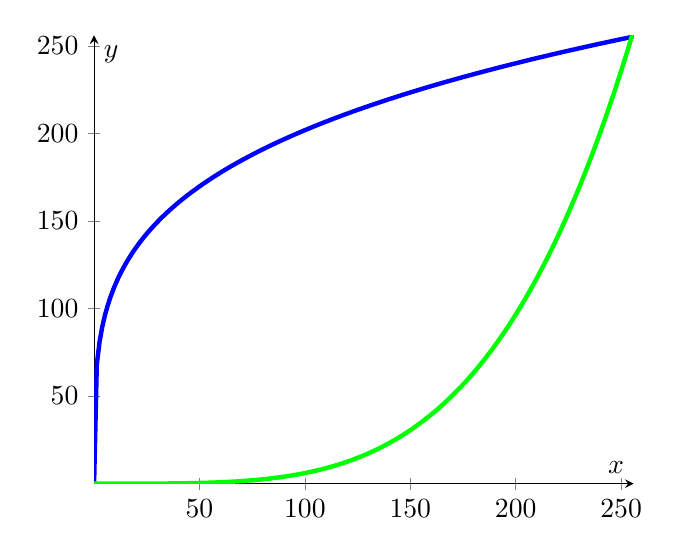
\begin{tikzpicture}[scale=01.0]
        \begin{axis}[
            axis x line=middle,
            axis y line=middle,
            ymin=0,ymax=256,ylabel=$y$,
            xmin=0,xmax=256,xlabel=$x$
            ]
        \addplot[domain=0:256, blue, ultra thick, samples=200] {255*(x/255)^0.25};
        \addplot[domain=0:256, green, ultra thick, samples=200] {255*(x/255)^4.0};
    \end{axis}
    \end{tikzpicture}
\caption{Graph of gamma function $(L-1)\left(\frac{r}{L-1}\right)^\gamma$ where $\gamma = 4$ (green) and $\gamma = \frac{1}{4}$ (blue).}
\label{fig:gamma}
\end{figure}

\begin{exmp}
    Contrast-enhancement: $T: r \mapsto c + c\sin\left(\frac{\pi(r-c)}{2c}\right)$ where $c = \frac{L - 1}{2}$. When $\gamma > 1$ the image is darkened, when $\gamma < 1$ the image is brightened, and when $\gamma = 1$ the image is unchanged.
\end{exmp}

\begin{figure}[ht!]
    \centering
    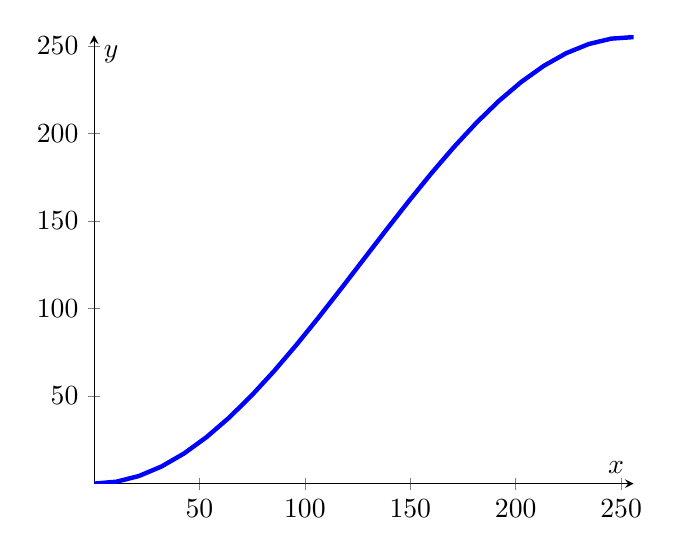
\begin{tikzpicture}[scale=01.0]
        \begin{axis}[
            axis x line=middle,
            axis y line=middle,
            ymin=0,ymax=256,ylabel=$y$,
            xmin=0,xmax=256,xlabel=$x$
            ]
        \addplot[domain=0:256, blue, ultra thick] {127.5 + 127.5*sin(deg(0.5*pi*(x - 127.5)/127.5))};
    \end{axis}
    \end{tikzpicture}
\caption{Graph of contrast enhancement $c + c\sin\left(\frac{\pi(r-c)}{2c}\right)$.}
\label{fig:contrast}
\end{figure}

\end{document}


\end{document}
